%% LaTeX preamble 
\documentclass[11pt,openany]{book}\usepackage[]{graphicx}\usepackage[]{color}
%% maxwidth is the original width if it is less than linewidth
%% otherwise use linewidth (to make sure the graphics do not exceed the margin)
\makeatletter
\def\maxwidth{ %
  \ifdim\Gin@nat@width>\linewidth
    \linewidth
  \else
    \Gin@nat@width
  \fi
}
\makeatother

\definecolor{fgcolor}{rgb}{0.345, 0.345, 0.345}
\newcommand{\hlnum}[1]{\textcolor[rgb]{0.686,0.059,0.569}{#1}}%
\newcommand{\hlstr}[1]{\textcolor[rgb]{0.192,0.494,0.8}{#1}}%
\newcommand{\hlcom}[1]{\textcolor[rgb]{0.678,0.584,0.686}{\textit{#1}}}%
\newcommand{\hlopt}[1]{\textcolor[rgb]{0,0,0}{#1}}%
\newcommand{\hlstd}[1]{\textcolor[rgb]{0.345,0.345,0.345}{#1}}%
\newcommand{\hlkwa}[1]{\textcolor[rgb]{0.161,0.373,0.58}{\textbf{#1}}}%
\newcommand{\hlkwb}[1]{\textcolor[rgb]{0.69,0.353,0.396}{#1}}%
\newcommand{\hlkwc}[1]{\textcolor[rgb]{0.333,0.667,0.333}{#1}}%
\newcommand{\hlkwd}[1]{\textcolor[rgb]{0.737,0.353,0.396}{\textbf{#1}}}%
\let\hlipl\hlkwb

\usepackage{framed}
\makeatletter
\newenvironment{kframe}{%
 \def\at@end@of@kframe{}%
 \ifinner\ifhmode%
  \def\at@end@of@kframe{\end{minipage}}%
  \begin{minipage}{\columnwidth}%
 \fi\fi%
 \def\FrameCommand##1{\hskip\@totalleftmargin \hskip-\fboxsep
 \colorbox{shadecolor}{##1}\hskip-\fboxsep
     % There is no \\@totalrightmargin, so:
     \hskip-\linewidth \hskip-\@totalleftmargin \hskip\columnwidth}%
 \MakeFramed {\advance\hsize-\width
   \@totalleftmargin\z@ \linewidth\hsize
   \@setminipage}}%
 {\par\unskip\endMakeFramed%
 \at@end@of@kframe}
\makeatother

\definecolor{shadecolor}{rgb}{.97, .97, .97}
\definecolor{messagecolor}{rgb}{0, 0, 0}
\definecolor{warningcolor}{rgb}{1, 0, 1}
\definecolor{errorcolor}{rgb}{1, 0, 0}
\newenvironment{knitrout}{}{} % an empty environment to be redefined in TeX

\usepackage{alltt}
\usepackage[utf8]{inputenc} 
\usepackage{amssymb, amsmath, amsthm}
\usepackage{fullpage}
\usepackage{setspace}
\usepackage{graphicx}
\usepackage{natbib}
\usepackage{rotating}
\usepackage{caption}
\usepackage{subcaption}
\usepackage{multirow}
\usepackage{booktabs}
\usepackage{dcolumn}
\usepackage[grey]{quotchap}
\usepackage{xcolor}
\usepackage[left=1in, top=1in, right=1.5in, bottom=1in, headsep=.5in]
{geometry}
\usepackage{fancyhdr, blindtext}
\usepackage{diagbox}
\usepackage{hyperref} 
\usepackage{placeins}
\renewenvironment{knitrout}{\begin{singlespace}}{\end{singlespace}}
\newcommand*{\mybox}[2]{\colorbox{#1!30}{\parbox{.98\linewidth}{#2}}}
\newcommand*{\befehl}[1]{\texttt{\textbackslash #1}} % Added by 


\fancyhf{}
\fancyhead[LE]{\slshape \rightmark} 
\fancyhead[RE]{\thepage}
\fancyhead[RO]{\slshape \leftmark} 
\fancyhead[LO]{\thepage}
\renewcommand{\headrulewidth}{0.4pt}
\pagestyle{fancy}
%% new command for greybox
\long\def\greybox#1{%
    \newbox\contentbox%
    \newbox\bkgdbox%
    \setbox\contentbox\hbox to \hsize{%
        \vtop{
            \kern\columnsep
            \hbox to \hsize{%
                \kern\columnsep%
                \advance\hsize by -2\columnsep%
                \setlength{\textwidth}{\hsize}%
                \vbox{
                    \parskip=\baselineskip
                    \parindent=0bp
                    #1
                }%
                \kern\columnsep%
            }%
            \kern\columnsep%
        }%
    }%
    \setbox\bkgdbox\vbox{
        \pdfliteral{0.85 0.85 0.85 rg}
        \hrule width  \wd\contentbox %
               height \ht\contentbox %
               depth  \dp\contentbox
        \pdfliteral{0 0 0 rg}
    }%
    \wd\bkgdbox=0bp%
    \vbox{\hbox to \hsize{\box\bkgdbox\box\contentbox}}%
    \vskip\baselineskip%
}
%% make greybox (grbox) a float
\usepackage{float}
\newfloat{grbox}{thp}{lop}[section]
\floatname{grbox}{Grey Box}
\IfFileExists{upquote.sty}{\usepackage{upquote}}{}
\begin{document}
\SweaveOpts{concordance=TRUE}



\title{Quantitative Research Methods for Political Science, Public Policy and Public Administration: 3rd Edition\\
  \LARGE With Applications in \texttt{R}}

\author{Hank C. Jenkins-Smith\\ 
Joseph T. Ripberger\\
Gary Copeland\\
Matthew C. Nowlin\\
Tyler Hughes\\
Aaron L. Fister\\
Wesley Wehde}

\date{\today}

\maketitle

\pagenumbering{roman} 

%% copyright page 

%% preface 
%%Added for third edition
\newpage
\chapter*{Copyright Page}

This work is licensed under a \href{https://creativecommons.org/licenses/by/4.0/}{Creative Commons Attribution 4.0 International License} (CC BY 4.0). You can download this book for free at: \url{https://shareok.org/handle/11244/52244}.  

\begin{figure}[h]
\centerline{\includegraphics[totalheight=1cm]{"CCicon".png}}
\label{fig:cc}
\end{figure}

%% table of contents 

{\singlespacing
  \tableofcontents
  
  \listoftables
 % \listoffigures
  }

% this sets the global options for knitR  


\newpage
\chapter*{Preface and Acknowledgments to the 3rd Edition}
The idea for this book grew over decades of teaching introductory and intermediate quantitative methods classes for graduate students in Political Science and Public Policy at the University of Oklahoma, Texas A\&M, and the University of New Mexico. Despite adopting (and then discarding) a wide range of textbooks, we were frustrated with inconsistent terminology, misaligned emphases, mismatched examples and data, and (especially) poor connections between the presentation of theory and the practice of data analysis. The cost of textbooks and the associated statistics packages for students seemed to us to be, frankly, outrageous. So, we decided to write our own book that students can download as a free PDF, and to couple it with \texttt{R}, an open-source (free) statistical program, and data from the Meso-Scale Integrated Socio-geographic Network (M-SISNet), a quarterly survey of approximately 1,500 households in Oklahoma that is conducted with support of the National Science Foundation (Grant No. IIA-1301789). Readers can learn about and download the data at \url{http://crcm.ou.edu/epscordata/}.

By intent, this book represents an open-ended group project that changes over time as new ideas and new instructors become involved in teaching graduate methods in the University of Oklahoma Political Science Department. The first edition of the book grew from lecture notes and slides that Hank Jenkins-Smith used in his methods classes. The second edition was amended to encompass material from Gary Copeland’s introductory graduate methods classes. The third edition (this one!) was updated by Joseph Ripberger, who currently manages and uses the book in his introductory and intermediate quantitative methods courses for Ph.D. students in the University of Oklahoma Political Science Department.

In addition to instructors, the graduate assistants who co-instruct the methods courses are an essential part of the authorship team. The tradition started with Dr. Matthew Nowlin, who assisted in drafting the first edition in \LaTeX. Dr. Tyler Hughes and Aaron Fister were instrumental in implementing the changes for the second edition. Wesley Wehde, the current co-instructor, is responsible for much of the third edition. 

This book, like politics and policy, constantly changes. Keep an eye on our \texttt{GitHub} repository (\url{https://github.com/ripberjt/qrmtextbook}) for modifications and additions. You never know what you might find peering back at you.\\

\noindent Hank Jenkins-Smith\\
Joseph Ripberger\\
Gary Copeland\\
Matthew Nowlin\\
Tyler Hughes\\
Aaron Fister\\
Wesley Wehde\\

\pagenumbering{arabic} 

%% chapters

\doublespace 
\part{Theory and Empirical Social Science} 




\chapter{Theories and Social Science}

The focus of this book is on using quantitative empirical research to test hypotheses and build theory in political science and public policy. The book is designed to be used by graduate students in the introductory and intermediate quantitative analysis courses. It is important to note that quantitative analysis is not the only -- or even the most important -- kind of analysis undertaken in political science and public policy research. Qualitative analysis, including ethnographic studies, systematic cases analyses, focus groups, archival studies, and qualitative elite interviews (to name only a few approaches) are of critical importance for understanding social and political phenomena. With that understanding in mind, this book and the associated courses focus on  the development and application of systematic analysis, hypothesis testing and theory building using quantitative data and modeling. Specifically, we focus on developing research design, univariate analysis, and an understanding of linear regression modeling and analysis (and related techniques). Throughout we provide with applications and examples using the \textbf{R} statistical platform. 


\section{The Scientific Method}

Empirical research, as outlined in this book, is based on the scientific method. Science is a particular way that some  epistemologists believe we can understand the world around us. Science, as a method, relies on both logic, as  captured by theory, and empirical observation of the world to determine whether the theory we have developed  conforms to what we actually observe. We seek to explain the world with our theories, and we test our theories by  deducing and testing hypotheses. When a \textbf{working hypothesis} is supported, we have more confidence in our theory. When the \textbf{null hypothesis} is supported, it undermines our proposed theory.

Science seeks a particular kind of knowledge and has certain biases. When we are engaging in scientific research  we are interested in reaching generalizations. Rather than wanting to explain why President Trump's approval dropped,  we are interested in explaining why presidential approval drops across various presidents, or, better yet, how economic  conditions affect presidential approval. These generalizations should be logical (which is nothing more than saying they  should be grounded in a strong theory) and they should be empirically verified (which, we will see means that we have  tested hypotheses deduced from our theory). We also look for generalizations that are causal in nature. Scientists actively seek explanations grounded in causation rather than correlation. Scientific knowledge should be replicable -- meaning that other scholars should be able to reach the same conclusions that you do. There should be inter-subjective agreement on scientific findings -- meaning that people, with different personal experiences and biases, should still reach the same conclusion.

Scientists also tend to prefer simple explanations to complex ones. They have a bias that says the world is pretty simple and that our theories should reflect that belief. Of course, people are complex, so in the social sciences it can be dangerous to look only for the simplest explanation as most concepts we consider have multiple causes.

\section{Theory and Empirical Research}

This book is concerned with the connection between theoretical claims and empirical data. It is about using statistical modeling; in particular, the tool of regression analysis, which is used to develop and refine theories. We define \textbf{theory} broadly as a set of interrelated propositions that seek to explain and, in some cases, predict an observed phenomenon. 
\begin{quote}
\begin{description}
\item[Theory] A set of interrelated propositions that seek to 
  explain and predict an observed phenomenon.
\end{description}
\end{quote}

\noindent Theories contain three important characteristics that we discuss in detail below. 

\begin{grbox}
  \greybox{\textbf{Characteristics of Good Theories}\\
\begin{itemize}
\item Coherent and internally consistent 
\item Causal in nature  
\item Generate testable hypotheses   
\end{itemize}}
\end{grbox}

\subsection{Coherent and Internally Consistent}

The set of interrelated propositions that constitute a well structured theory are based on \textbf{concepts}. In well-developed theories, the expected relationships among these concepts are both coherent and internally consistent. \textbf{Coherence} means the identification of concepts and the specified relationships among them are logical, ordered, and integrated. An \textbf{internally consistent} theory will explain relationships with respect to a set of common underlying causes and conditions, providing for consistency in expected relationships (and avoidance of contradictions). For systematic quantitative research, the relevant theoretical concepts are defined such that they can be measured and quantified. Some concepts are relatively easy to quantify, such as the number of votes cast for the winning Presidential candidate in a specified year or the frequency of arrests for gang-related crimes in a particular region and time period. Others are more difficult, such as the concepts of democratization, political ideology or presidential approval. Concepts that are more difficult to measure must be carefully \textbf{operationalized}, which is a process of relating a concept to an observation that can be measured using a defined procedure. For example, political ideology is often operationalized through public opinion surveys that ask respondents to place themselves on a Likert-type scale of ideological categories. 

\subsubsection{Concepts and Variables}
A concept is a commonality across observed individual events or cases. It is a regularity that we find in complex world. Concepts are our  building blocks to understanding the world and to developing theory that explains the world. Once we have identified concepts  we seek to explain them by developing theories based on them. Once we have explained a concept we need to define it. We do so in two steps. First, we give it a dictionary-like definition, called a nominal definition. Then, we develop an operational definition that identifies how we can measure and quantify it. 

Once a concept has been quantified, it is employed in modeling as a \textbf{variable}. In statistical modeling, variables are thought of as either dependent or independent variables. A \textbf{dependent variable}, $Y$, is the outcome variable; this is the concept we are trying to explain and/or predict. The \textbf{independent variable(s)}, $X$, is the variable(s) that is used to predict or explain the dependent variable. The expected relationships between (and among) the variables are specified by the theory.

\subsubsection{Measurement}

When measuring concepts, the indicators that are used in building and testing theories should be both \textbf{valid} and \textbf{reliable}. Validity
refers to how well the measurement captures the concept. Face validity, for example, refers to the plausibility and general acceptance of the measure, while the domain validity of the measure concerns the degree to which it captures all relevant aspects of the concept. Reliability, by contrast, refers to how consistent the measure is with repeated applications. A measure is reliable if, when applied to the repeated observations in similar settings, the outcomes are consistent.

\subsubsection{Assessing the Quality of a Measure}
Measurement is the process of assigning numbers to the phenomenon or concept that you are interested in. Measurement is straight-forward when we can directly observe the phenomenon. One agrees on a metric, such as inches or pounds, and then figures out how many of those units are present for the case in question. Measurement becomes more challenging when you cannot directly observe the concept of interest. In political science and public policy, some of the things we want to measure are directly observable: how many dollars were spent on a project or how many votes the incumbent receives, but many of our concepts are not observable: is issue X on the public's agenda, how successful is a program, or how much do citizens trust the president. When the concept is not directly observable the operational definition is especially important. The operational definition explains exactly what the researcher will do to assign a number for each subject/case. 

In reality, there is always some possibility that the number assigned does not reflect the true value for that case, i.e., there may be some error involved. Error can come about for any number of reasons, including mistakes in coding, the need for subjective judgments, or a measuring instrument that lacks precision. These kinds of error will generally produce inconsistent results; that is, they reduce reliability. We can assess the reliability of an indicator using one of two general approaches. One approach is a test-retest method where the same subjects are measured at two different points in time. If the measure is reliable the correlation between the two observations should be high. We can also assess reliability by using multiple indicators of the same concept and determining if there is a strong inter-correlation among them using statistical formulas such as Cronbach's alpha or Kuder-Richardson Formula 20 (KR-20).

We can also have error when our measure is not valid. Valid indicators measure the concept we think they are measuring. The indicator should both converge with the concept and discriminate between the concept and similar yet different concepts. Unfortunately there is no failsafe way to determine whether an indicator is valid. There are, however, a few things you can do to gain confidence in the validity of the indicator. First, you can simply look at it from a logical perspective and ask if it seems like it is valid. Does it have face validity?  Second, you can see if it correlates well with other indicators that are considered valid, and in ways that are consistent with theory. This is called construct validity. Third, you can determine if it works in the way expected, which is referred to as predictive validity. Finally, we have more confidence if 
other researchers using the same concept agree that the indicator is considered valid. This consensual validity at least ensures that different researchers are talking about the same thing.

\subsubsection{Measurement of Different Kinds of Concepts}
Measurement can be applied to different kinds of concepts, which causes measures of different concepts to vary. There are three primary \textbf{levels of measurement}; ordinal, interval, and nominal. \textbf{Ordinal level} measures indicate relative differences, such as more or less, but do not provide equal distances between intervals on the measurement scale. Therefore, ordinal measures cannot tell us \textit{how much} more or less one observation is than another. Imagine a survey question asking respondents to identify their annual income. Respondents are given a choice of five different income levels:  \$0-20,000, \$20,000-50,000, \$50,000-\$100,000, and \$100,000+. This measure gives us an idea of the rank order of respondents' income, but it is impossible for us to identify consistent differences between these responses. With an \textbf{interval level} measure, the variable is ordered and the differences between values are consistent. Sticking with the example of income, survey respondents are now asked to provide their annual income to the nearest ten thousand dollar mark (e.g., \$10,000, \$20,000, \$30,000, ect.). This measurement technique produces an interval level variable because we have both a rank ordering and equal spacing between values. Ratio scales are interval measures with the special characteristic that the value of zero (0) indicates the absence of some property. A value of zero (0) income in our example may indicate a person does not have a job. Another example of a ratio scale is the Kelvin temperature scale, because zero (0) degrees Kelvin indicates the complete absence of heat. Finally, a \textbf{nominal level} measure identifies categorical differences among observations. Numerical values assigned to nominal variables have no inherent meaning, but only differentiate one ``type" (e.g., gender, race, religion) from another.

\subsection{Theories and Causality}

Theories should be causal in nature, meaning that an independent variable is thought to have a causal influence on the dependent variable. In other words, a change in the independent variable \textit{causes} a change in the dependent variable. Causality can be thought of as the ``motor" that drives the model and provides the basis for explanation and (possibly) prediction.
\subsubsection{The Basis of Causality in Theories}
  \begin{enumerate}
  \item Time Ordering: The cause precedes the effect, $X \rightarrow Y$
  \item Co-Variation: Changes in $X$ are associated with changes in $Y$
  \item Non-Spuriousness: There is not a variable $Z$ that causes both
    $X$ and $Y$  
  \end{enumerate}

To establish causality we want to demonstrate that a change in the independent variable is a necessary and sufficient condition for a change in the dependent variable (though more complex, interdependent relationships can also be quantitatively modeled). We can think of the independent variable as a treatment, $\tau$, and we speculate that $\tau$ causes a change in our dependent variable, $Y$. The ``gold standard'' for casual inference is an experiment where a) the level of $\tau$ is controlled by the researcher and b) subjects are randomly assigned to a treatment or control group. The group that receives the treatment has outcome $Y_1$ and the control group has outcome $Y_0$; the treatment effect can be defined as $\tau = Y_1-Y_0$. Causality is inferred because the treatment was only given to one group, and since these groups were randomly assigned other influences should wash out. Thus the difference $\tau = Y_1-Y_0$ can be attributed to the treatment.

Given the nature of social science and public policy theorizing, we often can't control the treatment of interest. For example, our case study in this text concerns the effect of political ideology on views about the environment. For this type of relationship, we cannot randomly assign ideology in an experimental sense. Instead, we employ statistical controls to account for the possible influences of confounding factors, such as age and gender. Using multiple regression we control for other factors that might influence the dependent variable.\footnote{This matter will be discussed in more detail in the multiple regression section.}

\subsection{Generation of Testable Hypothesis}

Theory building is accomplished through the testing of hypotheses derived from theory. In simple form, a theory implies (sets of) relationships
among concepts. These concepts are then operationalized. Finally, models are developed to examine how the measures are related. Properly specified
hypotheses can be tested with empirical data, which are derived from the application  of valid and reliable measures to relevant observations. The testing and re-testing of hypotheses develops levels of confidence that we can have for the core propositions that constitute the theory. In short, empirically grounded theories must be able to posit clear hypotheses that are testable. In this text, we discuss hypotheses and test them using relevant models and data. 

As noted above, this text uses the concepts of political ideology and views about the environment as a case study in order to generate and test hypotheses about the relationships between these variables. For example, based on popular media accounts, it is plausible to expect that political
conservatives are less likely to be concerned about the environment than political moderates or liberals. Therefore, we can pose the \textbf{working hypothesis} that measures of political ideology will be systematically related to measures of concern for the environment -- with conservatives showing less concern for the environment. In classical hypothesis testing, the working hypothesis is tested against a \textbf{null hypothesis}. A null hypothesis is an implicit hypothesis that posits the independent variable has no effect (i.e., null effect) on the dependent variable. In our example, the null hypothesis states ideology has no effect on environmental concern.  

\section{Theory and Functions}

Closely related to hypothesis testing in empirical research is the concept of functional relationships -- or functions. Hypotheses posit systematic relationships between variables, and those relationships are expressed as functions. For example, we can hypothesize that an individual's productivity is related coffee consumption (productivity is a \textit{function} of coffee consumption).\footnote{The more coffee, the greater the productivity -- up to a point! Beyond some level of consumption, coffee may induce the jitters and ADD-type behavior, thereby undercutting productivity. Therefore the posited function that links coffee consumption to productivity is non-linear, initially positive but then flat or negative as consumption increases.} 

Functions are ubiquitous. When we perceive relational order or patterns in the world around us, we are observing functions. Individual decisions about when to cross the street, whether to take a nap, or engage in a barroom brawl can all be ascribed to patterns (the ``walk" light was lit; someone stayed up too late last night; a Longhorn insulted the Sooner football team). Patterns are how we make sense of the world, and patterns are expressed as functions. That does not mean the functions we perceive are always correct, or that they allow us to predict perfectly. However, without functions we don't know what to expect; chaos prevails. 

In mathematical terms, a function relates an outcome variable, $y$, to one or more inputs, $x$. This can be expressed more generally as: $y=f(x_{1},x_{2},x_{3},... x_{n})$, which means $y$ is `a function of the $x$'s, or, $y$ varies as a function of the $x$'s. 

Functions form the basis of the statistical models that will be developed throughout the text. In particular, this text will focus on
linear regression, which is based on linear functions such as $y=f(x)=5+x$, where $5$ is a constant and $x$ is a variable. We can plot this function with the values of $x$ ranging from $-5$ to $5$. This is shown in Figure \ref{figfun1}. 



\begin{figure}
  \centering
  \caption{Linear Function \\ $y=f(x)=5+x$  \label{figfun1}}
  \includegraphics[width=0.4\textwidth]%
    {01_Theory/fun1.pdf}% picture filename
\end{figure}

As you can see, the $x$ values range from $-5$ to $5$ and the corresponding $y$ values range from $0$ to $10$. The function produces a straight line because the changes in $y$ are consistent across all values of $x$. This type of function is the basis of the linear models we will develop, therefore these models are said to have a \textbf{linear functional form}. 

However, non-linear functional forms are also common. For example,  $y=f(x)=3-x^2$ is a quadratic function, which is a type of polynomial function since it contains a square term (an exponent). It is plotted in Figure \ref{figfun2}. This function is non-linear because the changes in $y$ are not consistent across the full range of $x$.



\begin{figure}
  \centering
  \caption{Non-Linear Function: One Exponent \\ $y=f(x)=3-x^2$ \label{figfun2}}
  \includegraphics[width=0.4\textwidth]%
    {01_Theory/fun2.pdf}% picture filename
\end{figure}

\subsubsection{Examples of Functions in Social Science Theories}

As noted, functions are the basis of statistical models that are used to test hypotheses. Below are a few examples of functions that are related to social science theories. 
\begin{itemize}
  \item Welfare and work incentives
    \begin{itemize}
    \item Employment $= f$(welfare programs, education level, work experience,...) 
    \end{itemize}
\item Nuclear weapons proliferation
  \begin{itemize}
  \item Decision to develop nuclear weapons $= f$(perceived threat,
    incentives, sanctions,...) 
  \end{itemize}
\item   ``Priming'' and political campaign contributions
  \begin{itemize}
  \item Contribution(\$) $= f$(Prime (suggested \$), income,...)
  \end{itemize}
\item  Successful program implementation
  \begin{itemize}
  \item Implementation $= f$(clarity of law, level of public support, problem complexity,...) \
  \end{itemize}
\end{itemize}

Try your hand at this with theories that are familiar to you. First, identify the dependent and independent variables of interest; then develop your own conjectures about the form of the functional relationship(s) among them.

\section{Theory in Social Science}

Theories play several crucial roles in the development of scientific knowledge. Some of these include providing patterns for data interpretation, linking the results of related studies together, providing frameworks for the study of concepts, and allowing the interpretation of more general meanings from any single set of findings. Hoover and Todd (2004) provide a very useful discussion of the role of theories in ``scientific thinking" -- find it and read it!
\begin{grbox}
  \greybox{\textbf{The Role of Theory in Social Science}\\
      \scriptsize{Adapted from \textit{The Elements of Social Scientific
          Thinking} by Kenneth Hoover and Todd Donovan (2004, 37)}
      \normalsize 
        \begin{itemize}
        \item Theory provides patterns for the interpretation of data
        \item Theory links one study with another 
        \item Theory supplies frameworks within which concepts acquire significance
        \item Theory allows us to interpret the larger meaning of our findings   
        \end{itemize}}
\end{grbox}
Perhaps, in the broadest sense, theories tie the enterprise of the social (or any) science together, as we build, revise, criticize and destroy theories in that collective domain referred to as ``the literature."

\section{Outline of the Book}

The goal of this text is to develop an understanding of how to build theories by testing hypotheses using empirical data and statistical models. There are three necessary ingredients of strong empirical research. The first is a carefully constructed theory that generates empirically testable hypotheses. Once tested, these hypothesis should have implications for the development of theory. The second ingredient is quality data. The data should be valid, reliable, and relevant. The final ingredient is using the appropriate model design and execution. Specifically, the appropriate statistical models must be used  to test the hypotheses. Appropriate models are those that are properly specified, estimated, and use data that conforms to the statistical assumptions. This course focuses on model design and execution.

As noted, this text uses political ideology and views on the environment as a case study to examine theory building in the social sciences.\footnote{As you may have already realized, social scientists often take these steps out of order ... we may ``back into" an insight, or skip a step and return to it later. There is no reliable cookbook for what we do. Rather, think of the idealized steps of the scientific process as an important heuristic that helps us think through our line of reasoning and analysis -- often after the fact -- to help us be sure that we learned what we \textit{think} we learned from our analysis.} The text is organized by the idealized steps of the research process. As a first step, this first chapter discussed theories and hypothesis testing, which should always be (but often are not!) the first consideration. The second chapter focuses on research design and issues of internal and external validity. Chapter 3 examines data and covers specific ways to understand how the variables in the data are distributed. This is vital to know before doing any type of statistical modeling. The fourth chapter is an introduction to probability. The fifth chapter covers inference and how to reach conclusions regarding a population when you are studying a sample. The sixth chapter explores how to understand basic relationships that can hold between two variables including cross tabulations, covariance, correlation, and difference of means tests. These relationships are the foundation of more sophisticated statistical approaches and therefore understanding these relationships is often a precursor to the later steps of statistical analysis. The seventh through tenth chapters focus on bivariate ordinary least squares (OLS) regression, or OLS regression with a dependent variable and one independent variable. This allows us to understand the mechanics of regression before moving on the third section (chapters eleven to fifteen) that cover multiple OLS regression. The final section of the book (chapter sixteen) covers logistic (logit) regression. Logit regression is an example of a class of models called generalized linear models (GLM). GLMs allow for linear analysis to be performed on different types of dependent variables that may not be appropriate for OLS regression.

As a final note, this text makes extensive use of \texttt{R}. The code to reproduce all of the examples is excluded in the text in such a way that it can be easily copied and pasted into your \texttt{R} console. The data used for the examples is available as well. You can find it here: http://crcm.ou.edu/epscordata/.



%Chapter 2 is from Gary
\chapter{Research Design}

Research design refers to the plan to collect information to address your research question. It covers the set of procedures that are used to collect your data and how your data will be analyzed. Your research plan identifies what type of design you are using. Your plan should make clear what your research question is, what theory or theories will be considered, key concepts, your hypotheses, your independent and dependent variables, their operational definitions, your unit of analysis, and what statistical analysis you will use. It should also address the strengths and weaknesses of your particular design. The major design categories for scientific research are \textit{experimental designs} and \textit{observational designs}. The latter is some times referred to as a correlational research design.

\section{Overview of the Research Process} 

Often scholars rely on data collected by other researchers and end up, de facto, with the research design developed by the original scholars. But if you are collecting your own data this stage becomes the key to the success of your project and the decisions you make at this stage will determine both what you will be able to conclude and what you will not be able to conclude. It is at this stage that all the elements of science come together. 

We can think of research as starting with a problem or a \textbf{research question} and moving to an attempt to provide an answer to that problem by developing a theory. If we want to know how good (empirically accurate) that theory is we will want to put it to one or more tests. Framing a research question and developing a theory could all be done from the comforts of your backyard hammock. Or, they could be done by a journalist (or, for that matter, by the village idiot) rather than a scientist. To move beyond that stage requires more. To test the theory, we deduce one or more hypotheses from the theory, i.e., statements that should be true if the theory accurately depicts the world. We test those hypotheses by systematically observing the world---the empirical end of the scientific method.  It requires you to get out of that hammock and go observe the world. The observations you make allow you to accept or reject your hypothesis, providing insights into the accuracy and value of your theory. Those observations are conducted according to a plan or a research design. 

\section{Internal and External Validity}

Developing a research design should be more than just a matter of convenience (although there is an important element of that as we will discuss at the end of this chapter). Not all designs are created equally and there are trade-offs we make when opting for one type of design over another. The two major components of an assessment of a research design are its internal validity and its external validity. \textbf{Internal validity} basically means we can make a causal statement within the context of our study. We have internal validity if, for our study, we can say our independent variable caused our dependent variable. To make that statement we need to satisfy the conditions of causality we identified previously. The major challenge is the issue of \textbf{spuriousness}. We have to ask if our design allows us to say our independent variable makes our dependent variable vary systematically as it changes and that those changes in the dependent variable are not due to some third or extraneous factor.  It is worth noting that even with internal validity, you might have serious problems when it comes to your theory. Suppose your hypothesis is that being well-fed makes one more productive. Further suppose that you operationalize ``being well-fed" as consuming twenty Hostess Twinkies in an hour. If the Twinkie eaters are more productive those who did not get the Twinkies your might be able to show causality, but if your theory is based on the idea that ``well-fed" means a balanced and healthy diet then you still have a problematic research design. It has internal validity because what you manipulated (Twinkie eating) affected your dependent variable, but that conclusion does not really bring any enlightenment to your theory.

The second basis for evaluating your research design is to assess its \textbf{external validity}. External validity means that we can generalize the results of our study. It asks whether our findings are applicable in other settings. Here we consider what population we are interested in generalizing to. We might be interested in adult Americans, but if we have studied a sample of first-year college students then we might not be able to generalize to our target population. External validity means that we believe we can generalize to our (and perhaps other) population(s). Along with other factors discussed below, replication is a key to demonstrating external validity.

\section{Major Classes of Designs}

There are many ways to classify systematic, scientific research designs, but the most common approach is to classify them as experimental or observational. \textbf{Experimental designs} are most easily thought of as a standard laboratory experiment. In an experimental design the researcher controls (holds constant) as many variables as possible and then assigns subjects to groups, usually at random. If randomization works (and it will if the sample size is large enough, but technically that means infinite in size), then the two groups are identical. The researcher then manipulates the experimental treatment (independent variable) so that one group is exposed to it and the other is not. The dependent variable is then observed. If the dependent variable is different for the two groups, we can have quite a bit of confidence that the independent variable caused the dependent variable. That is, we have good internal validity. In other words, the conditions that need to be satisfied to demonstrate causality can be met with an experimental design. Correlation can be determined, time order is evident, and spuriousness is not problem---there simply is no alternative explanation.

Unfortunately, in the social sciences the artificiality of the experimental setting often creates suspect external validity. We may want to know the effects of a news story on views towards climate change so we conduct an experiment where participants are brought into a lab setting and some (randomly selected) see the story and others watch a video clip with a cute kitten. If the experiment is conducted appropriately, we can determine the consequences of being exposed to the story. But, can we extrapolate from that study and have confidence that the same consequences would be found in a natural setting, e.g., in one's living room with kids running around and a cold beverage in your hand? Maybe not. A good researcher will do things that minimize the artificiality of the setting, but external validity will often remain suspect. 
  
\textbf{Observational} designs tend to have the opposite strengths and weaknesses. In an observational design, the researcher cannot control who is exposed to the experimental treatment; therefore, there is no random assignment and there is no control. Does smoking cause heart disease?  A researcher might approach that research question by collecting detailed medical and life style histories of a group of subjects. If there is a correlation between those who smoke and heart disease, can we conclude a causal relationship?  Generally the answer to that question is ``no", because any other difference between the two groups is an alternative explanation meaning that the relationship might be spurious. For better or worse, though, there are fewer threats to external validity (see below for more detail) because of the natural research setting.
  
A specific type of observational design, the \textbf{natural experiment}, requires mention because they are increasingly used to great value. In a natural experiment, subjects are exposed to different environmental conditions that are outside the control of the researcher, but the process governing exposure to the different conditions arguably resembles random assignment. Weather, for example, is an environmental condition that arguably mimics random assignment. For example, imagine a natural experiment where one part of New York City gets a lot of snow on election day, whereas another part gets almost no snow. Researchers do not control the weather, but might argue that patterns of snowfall are basically random, or, at the very least, exogenous to voting behavior. If you buy this argument, then you might use this as natural experiment to estimate the impact of weather conditions on voter turnout. Because the experiment takes place in natural setting, external validity is less of a problem. But, since we do not have control over all events, we may still have internal validity questions.

\section{Threats to Validity}

To understand the pros and cons of various designs and to be able to better judge specific designs, we identify specific \textbf{threats to internal and external validity}. Before we do so, it is important to note that a (perhaps ``the") primary challenge to establishing internal validity in the social sciences is the fact that most of the phenomena we care about have multiple causes and are often a result of some complex set of interactions. For examples, $X$ may be only a partial cause of $Y$, or $X$ may cause $Y$, but only when $Z$ is present. Multiple causation and interactive affects make it very difficult to demonstrate causality, both internally and externally. Turning now to more specific threats, Table \ref{tab:ThreatIV} identifies common threats to internal validity and Table \ref{tab:ThreatEV} identifies common threats to external validity.
% Please add the following required packages to your document preamble:
% \usepackage{graphicx}
\begin{table}[h]
\caption{Common Threats to Internal Validity}
\label{tab:ThreatIV}
%\resizebox{\textwidth}{!}{%
\begin{tabular}{|p{4cm}|p{9cm}|}
\hline
Threat &  \\ \hline
History & Any event that occurs while the experiment is in progress might be an alternative explanation; using a control group mitigates this concern \\ \hline
Maturation & Normal changes over time (e.g. fatigue or aging) might affect the dependent variable; using a control group mitigates this concern \\ \hline
Selection Bias & If randomization is not used to assign participants, the groups may not be equivalent \\ \hline
Experimental Mortality & If groups lose participants (for example, due to dropping out of the experiment) they may not be equivalent \\ \hline
Testing & A pre-test may confound the influence of the experimental treatment; using a control group mitigates this concern \\ \hline
Instrumentation & Changes or differences in the process of measurement might alternatively account for differences \\ \hline
Statistical Regression & The natural tendency for extreme scores to regress or move towards the mean \\ \hline
\end{tabular}
%} removed due to \resizebox removed
\end{table}
\FloatBarrier

% Please add the following required packages to your document preamble:
% \usepackage{graphicx}
\begin{table}[h]
\caption{Major Threats to External Validity}
\label{tab:ThreatEV}
% \resizebox{\textwidth}{!}{%
\begin{tabular}{|p{4cm}|p{9cm}|}
\hline
Threat &  \\ \hline
Testing & Pre-testing or multiple measures may influence subsequent measurement \\ \hline
Interaction with Testing & A pre-test may sensitize subjects to the effects of the experimental treatment \\ \hline
Sample Representation & An unrepresentative sample will limited  the ability to draw inferences about the population \\ \hline
Interaction of Selection Bias and Experimental Treatment & A bias in selection may produce subjects that are more or less sensitive to the experimental treatment \\ \hline
Experimental Setting & The finding may not be transferable to a natural setting; knowledge of participation may produce a Hawthorne effect \\ \hline
\end{tabular}
%} removed due to not using \resizebox
\end{table}
\FloatBarrier

\section{Some Common Designs}

In this section we look at some common research designs, the notation used to symbolize them, and then consider the internal and external validity of the designs. We start with the most basic experimental design, the post-test only design Table \ref{tab:Experiment1}. In this design subjects are randomly assigned to one of two groups with one group receiving the experimental treatment.\footnote{The symbol R means there is random assignment to the group. X symbolizes exposure to the experimental treatment. O is an observation or measurement.}  There are advantages to this design in that it is relatively inexpensive and eliminates the threats associated with pre-testing. If randomization worked the (unobserved) pre-test measures would be the same so any differences in the observations would be due to the experimental treatment. The problem is that randomization could fail us, especially if the sample size is small.\\

\begin{table}[h]
\caption{Post-test Only (with a Control Group) Experimental Design} 
\label{tab:Experiment1}
\begin{tabular}{lll}
R & X & $O_1$ \\
R &  & $O_2$
\end{tabular}
\end{table}
\FloatBarrier

Many experimental groups are small and many researchers are not comfortable relying on randomization without empirical verification that the groups are the same, so another common design is the Pre-test, Post-test Design (Table \ref{tab:Experiment2}). By conducting a pre-test, we can be sure that the groups are identical when the experiment begins. The disadvantages are that adding groups drives the cost up (and/or decreases the size of the groups) and that the various threats due to testing start to be a concern. Consider the example used above concerning a news story and views on climate change. If subjects were given a pre-test on their views on climate change and then exposed to the news story, they might become more attentive to the story. If a change occurs, we can say it was due to the story (internal validity), but we have to wonder whether we can generalize to people who had not been sensitized in advance.

\begin{table}[h]
\caption{Pre-test, Post-Test (with a Control Group) Experimental Design} 
\label{tab:Experiment2}

\begin{tabular}{llll}
R & $O_1$ & X & $O_2$ \\
R & $O_3$ &  & $O_4$
\end{tabular}
\end{table}
\FloatBarrier


A final experimental design deals with all the drawbacks of the previous two by combining them into what is called the Solomon Four Group Design (Table \ref{tab:Experiment3}). Intuitively it is clear that the concerns of the previous two designs are dealt with in this design, but the actual analysis is complicated. Moreover, this design is expensive so while it may represent an ideal, most researchers find it necessary to compromise.

\begin{table}[h]
\caption{Solomon Four Group Experimental Design} 
\label{tab:Experiment3}
\begin{tabular}{llll}
R &  & X & $O_1$ \\
R &  &  & $O_2$ \\
R & $O_3$ & X & $O_4$ \\
R & $O_5$ &  & $O_6$
\end{tabular}
\end{table}
\FloatBarrier

Even the Solomon Four Group design does not solve all of our validity problems. It still likely suffers from the artificiality of the experimental setting. Researchers generally try a variety of tactics to minimize the artificiality of the setting through a variety of efforts such as watching the aforementioned news clip in a living room-like setting rather than on a computer monitor in a cubicle or doing jury research in the courthouse rather than the basement of a university building.

Observational designs lack random assignment, so all of the above designs can be considered observational designs when assignment to groups is not random. You might, for example, want to consider the affects of a new teaching style on student test scores. One classroom might get the intervention (the new teaching style) and another not be exposed to it (the old teaching style). Since students are not randomly assigned to classrooms it is not experimental and the threats that result from selection bias become a concern (along with all the same concerns we have in the experimental setting). What we gain, of course, is the elimination or minimization of the concern about the experimental setting.

A final design that is commonly used is the repeated measures or longitudinal research design where repeated observations are made over time and at some point there is an intervention (experimental treatment) and then subsequent observations are made (Table \ref{tab:Experiment4}).  Selection bias and testing threats are obvious concerns with this design. But there are also concerns about history, maturation, and mortality. Anything that occurs between $O_n$ and $O_{n+1}$ becomes an alternative explanation for any changes we find. This design may also have a control group, which would give clues regarding the threat of history. Because of the extended time involved in this type of design, the researcher has to concerned about experimental mortality and maturation. 

\begin{table}[h]
\caption{Repeated Measures Experimental Design}
\label{tab:Experiment4}
\begin{tabular}{lllllllll}
$O_1$ & $O_2$ & $O_3$ & $O_n$ & $X$ & $O_{n+1}$ & $O_{n+2}$ & $O_{n+2}$ & $O_{n+3}$
\end{tabular}
\end{table}
\FloatBarrier

This brief discussion illustrates major research designs and the challenges to maximizing internal and external validity.  With these experimental designs we worry about external validity, but since we have said we seek the ability to make causal statements, it seems that a preference might be given to research via experimental designs. Certainly we see more and more experimental designs in political science with important contributions. But, before we dismiss observational designs, we should note that in later chapters, we will provide an approach to providing statistical controls which, in part, substitutes for the control we get with experimental designs. 

\section{Plan Meets Reality}

Research design is the process of linking together all the elements of your research project. None of the elements can be taken in isolation, but must all come together to maximize your ability to speak to your theory (and research question) while maximizing internal and external validity within the constraints of your time and budget. The planning process is not straightforward and there are times that you will feel you are taking a step backwards. That kind of ``progress'' is normal. 
	
Additionally, there is no single right way to design a piece of research to address your research problem. Different scholars, for a variety of reasons, would end up with quite different designs for the same research problem. Design includes trade-offs, e.g., internal vs. external validity, and compromises based on time, resources, and opportunities. Knowing the subject matter -- both previous research and the subject itself -- helps the researcher understand where a contribution can be made and when opportunities present themselves.




\chapter{Exploring and Visualizing Data}



You have your plan, you carry out your plan by getting out and collecting your data, and then you put your data into a file.  You are excited to test your hypothesis so you immediately run your multiple regression analysis and look at your output.  You can do that (and probably will even if we advise against it), but what you need to do before you can start to make sense of that output is to look carefully at your data.  You will want to know things like ``how much spread do I have in my data" and ``do I have any outliers".  (If you have limited spread, you may discover that it is hard to explain variation in something that is nearly a constant and if you have an outlier, your statistics may be focused on trying to explain that one case.) 

In this chapter, we will identify the ways to characterize your data before you do serious analysis both to understand what you are doing statistically and to error-check.

\section{Characterizing Data}

What does it mean to characterize your data? First, it means knowing how many observations are contained in your data, and the distribution of those observations over the range of your variable(s). What kinds of measures (interval, ordinal, nominal) do you have, and what are the ranges of valid measures for each variable? How many cases of missing (no data) or mis-coded (measures that fall outside the valid range) do you have? What do the coded values represent? While seemingly trivial, checking and evaluating your data for these attributes can save you major headaches later. For example, missing values for an observation often get a special code -- say, ``-99" -- to distinguish them  from valid observations. If you neglect to treat these values properly, R (or any other statistics program) will treat that value as if it were valid and thereby turn your results into a royal hairball. We know of cases in which even seasoned quantitative scholars have made the embarrassing mistake of failing to properly handle missing values in their analyses. In at least one case, a published paper had to be retracted for this reason. So don't skimp on the most basic forms of data characterization!

The dataset used for purposes of illustration in this version of this text is taken from a survey of Oklahomans, conducted in 2016, by OU's Center for Risk and Crisis Management. The survey question wording and background will be provided in class. However, for purposes of this chapter, note that the measure of  \textbf{ideology} consists of a self-report of political ideology on a scale that ranges from 1 (strong liberal) to 7 (strong conservative); the measure of the \textbf{perceived risk of climate change} ranges from zero (no risk) to 10 (extreme risk). \textbf{Age} was measured in years. 

It is often useful to graph the variables in your data set to get a better idea of their distribution. In addition, we may want to compare the distribution of a variable to a theoretical distribution (typically a normal distribution). This can be accomplished in several ways, but we will show two here---a histogram and a density curve---and more will be discussed in later chapters. Here we examine the distribution of the variable measuring the perceived risk of climate change. The red line on the density visualization presents the normal distribution given the mean and standard deviation of our variable.
% Omitted: A histogram creates intervals of equal length, called bins, and displays the frequency of observations in each of the bins. To produce a histogram in R simply use the geom_histogram command in the \texttt{ggplot2} package. Next, we  plot the density of the observed data along with a normal curve.  This can be done with the \texttt{geom_density} command in the \texttt{ggplot2} package. 

%Note that the normal distribution overlay using the \texttt{stat_function} function for the \texttt{gccrsk} variable is based on the mean and standard deviation of the \textttt{age} variable. The results are shown in Figure \ref{fig:rsk_2}. As you can see, the \texttt{age} variable is not quite normally distributed.  The histogram illustrates that the majority of observations are contained in the upper half of the variable's range.  Moreover, the density curve indicates the the distribution if negatively skewed, and the peak of the distribution is higher on the \texttt{gccrsk} scale than that of the theoretical normal distribution.



\begin{knitrout}
\definecolor{shadecolor}{rgb}{0.969, 0.969, 0.969}\color{fgcolor}\begin{kframe}
\begin{alltt}
\hlkwd{ggplot}\hlstd{(ds,} \hlkwd{aes}\hlstd{(age))} \hlopt{+} \hlkwd{geom_histogram}\hlstd{()}
\hlkwd{dev.off}\hlstd{()}
\end{alltt}
\end{kframe}
\end{knitrout}

\begin{knitrout}
\definecolor{shadecolor}{rgb}{0.969, 0.969, 0.969}\color{fgcolor}\begin{kframe}
\begin{alltt}
\hlkwd{ggplot}\hlstd{(ds,} \hlkwd{aes}\hlstd{(age))} \hlopt{+} \hlkwd{geom_density}\hlstd{()} \hlopt{+} \hlkwd{stat_function}\hlstd{(}\hlkwc{fun} \hlstd{= dnorm,}
    \hlkwc{args} \hlstd{=} \hlkwd{list}\hlstd{(}\hlkwc{mean} \hlstd{=} \hlkwd{mean}\hlstd{(ds}\hlopt{$}\hlstd{age,} \hlkwc{na.rm} \hlstd{= T),} \hlkwc{sd} \hlstd{=} \hlkwd{sd}\hlstd{(ds}\hlopt{$}\hlstd{age,}
        \hlkwc{na.rm} \hlstd{= T)),} \hlkwc{color} \hlstd{=} \hlstr{"red"}\hlstd{)}
\hlkwd{dev.off}\hlstd{()}
\end{alltt}
\end{kframe}
\end{knitrout}


\begin{figure}
  \centering
  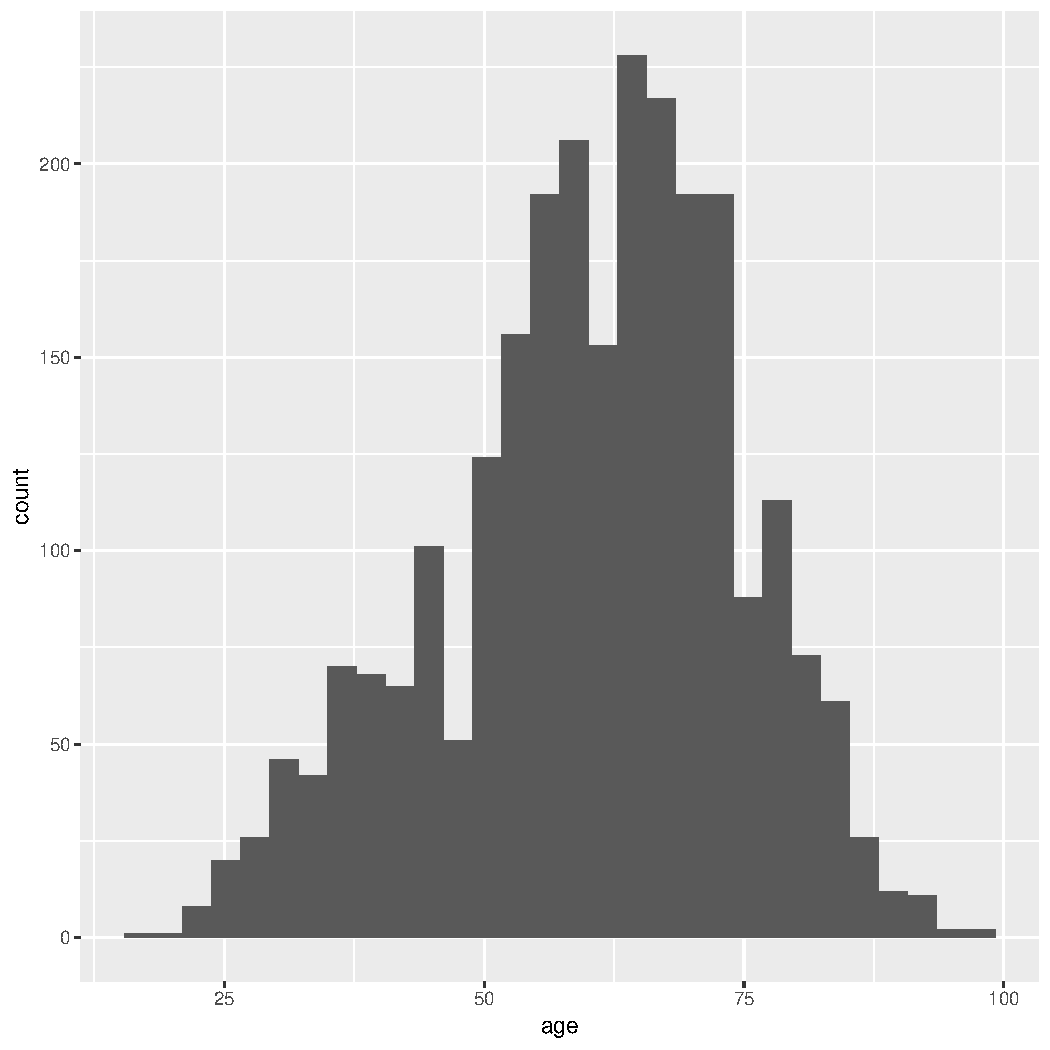
\includegraphics[width=.4\textwidth]{03_Data/rskhist.pdf}
  \caption{Histogram}
\end{figure}
\begin{figure}
  \centering
  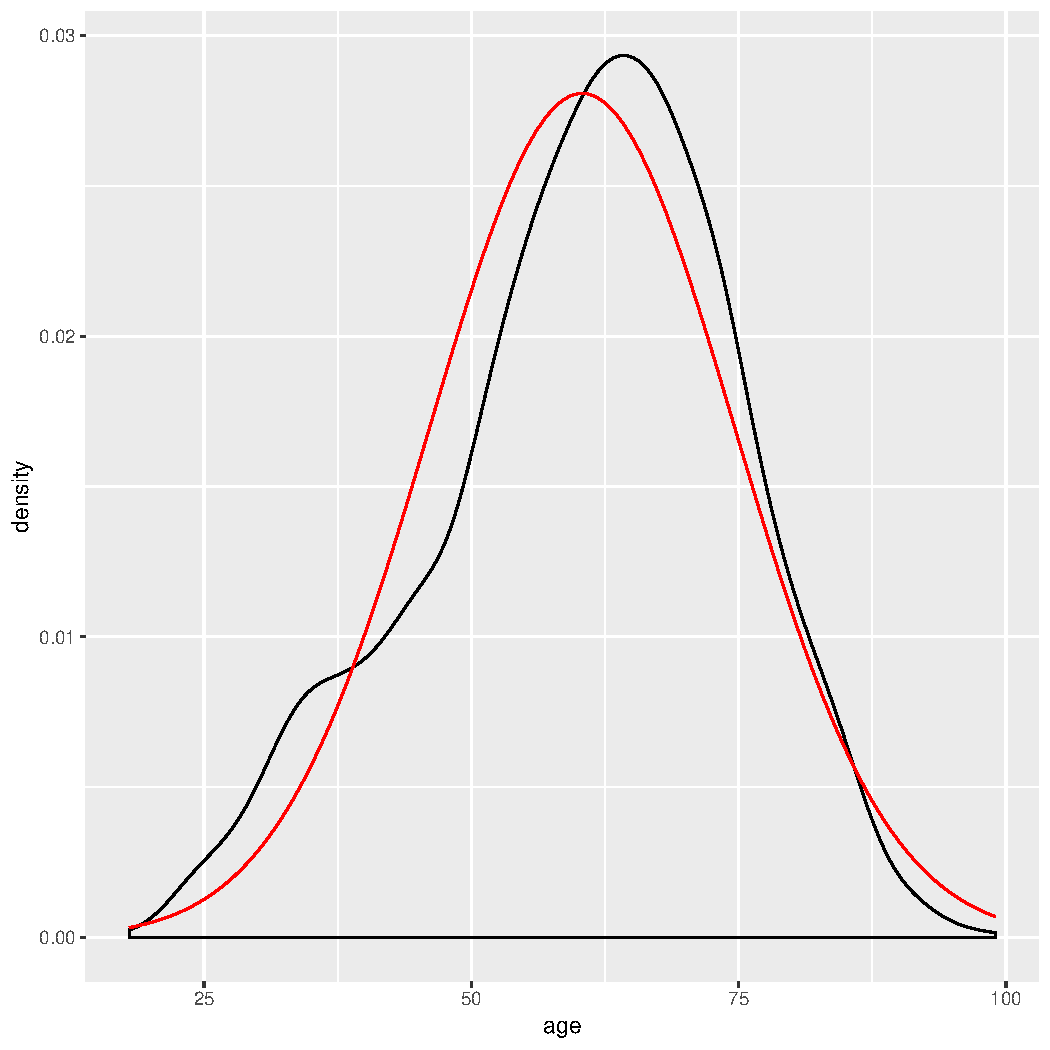
\includegraphics[width=.4\textwidth]{03_Data/rskden.pdf}
  \caption{Density Curve
  \label{fig:rsk_2}}
\end{figure}
  

You can also get an overview of your data using a table known as a frequency distribution. The frequency distribution summarizes how often each value of your variable occurs in the dataset.  If your variable has a limited number of values that it can take on, you can report all values, but if it has a large number of possible values (e.g., age of respondent), then you will want to create categories, or bins, to report those frequencies. In such cases, it is generally easier to make sense of the percentage distribution.  Table \ref{tab:ideology} is a frequency distribution for the ideology variable.  From that table we see, for example, that about one-third of all respondents are moderates. We see the numbers decrease as we move away from that category, but not uniformly.  There are a few more people on the conservative extreme than on the liberal side and that the number of people placing themselves in the penultimate categories on either end is greater than those towards the middle.  The histogram and density curve would, of course, show the same pattern.

The other thing to watch for here (or in the charts) is whether there is an unusual observation.  If one person scored 17 in this table, you could be pretty sure a coding error was made somewhere.  You cannot find all your errors this way, but you can find some, including the ones that have the potential to most seriously adversely affect your analysis.
  
\begin{table}[h]
\caption{Frequency Distribution for Ideology}
\label{tab:ideology}
\begin{tabular}{|l|c|c|c|}
\hline
Ideology & Frequency & Percentage & \begin{tabular}[c]{@{}c@{}}Cumulative \\ Percentage\end{tabular} \\ \hline
1 Strongly Liberal & 122 & 4.8 & 4.8 \\ \hline
2 & 279 & 11.1 & 15.9 \\ \hline
3 & 185 & 7.3 & 23.2 \\ \hline
4 & 571 & 22.6 & 45.8 \\ \hline
5 & 328 & 13.0 & 58.8 \\ \hline
6 & 688 & 27.3 & 86.1 \\ \hline
7 Strongly Conservative & 351 & 13.9 & 100.0 \\ \hline
Total & 2524 & 100 &  \\ \hline
\end{tabular}
\end{table}

\noindent In R, we can obtain the data for the above table with the following functions:

\begin{knitrout}
\definecolor{shadecolor}{rgb}{0.969, 0.969, 0.969}\color{fgcolor}\begin{kframe}
\begin{alltt}
\hlcom{# frequency counts for each level}
\hlkwd{table}\hlstd{(ds}\hlopt{$}\hlstd{ideol)}
\end{alltt}
\begin{verbatim}
## 
##   1   2   3   4   5   6   7 
## 122 279 185 571 328 688 351
\end{verbatim}
\begin{alltt}
\hlcom{# To view percentages}
\hlkwd{library}\hlstd{(dplyr)}
\hlkwd{table}\hlstd{(ds}\hlopt{$}\hlstd{ideol)} \hlopt \hlkwd{prop.table}\hlstd{()}
\end{alltt}
\begin{verbatim}
## 
##          1          2          3          4          5          6 
## 0.04833597 0.11053883 0.07329635 0.22622821 0.12995246 0.27258320 
##          7 
## 0.13906498
\end{verbatim}
\begin{alltt}
\hlcom{# multiply the numbers by 100}
\hlkwd{table}\hlstd{(ds}\hlopt{$}\hlstd{ideol)} \hlopt \hlkwd{prop.table}\hlstd{()} \hlopt{*} \hlnum{100}
\end{alltt}
\begin{verbatim}
## 
##         1         2         3         4         5         6         7 
##  4.833597 11.053883  7.329635 22.622821 12.995246 27.258320 13.906498
\end{verbatim}
\end{kframe}
\end{knitrout}


Having obtained a sample, it is important to be able to characterize that sample.  In particular, it is important to understand the probability distributions associated with each variable in the sample. 

\subsection{Central Tendency} 
Measures of central tendency are useful because a single statistic can  be used to describe the distribution. We focus on three measures of central
tendency; the mean, the median, and the mode.  

\begin{grbox}
 \greybox{\textbf{Measures of Central Tendency}
   \begin{itemize}
   \item The Mean: The arithmetic average of the values
   \item The Median: The value at the center of the distribution 
   \item The Mode: The most frequently occurring value  
   \end{itemize}}   
\end{grbox}

We will primarily rely on the mean, because of its efficient property of representing the data. But medians -- particularly when used in conjunction with the mean - can tell us a great deal about the shape of the distribution of our data. We will return to this point shortly.

\subsection{Level of Measurement and Central Tendency}

The three measures of central tendency --  the mean, median, and mode -- each tell us something different about our data, but each has some limitations (especially when used alone). Knowing the mode tells us what is most common, but we do not know how common and, using it alone, would not even leave us confident that it is an indicator of anything very \textit{central}. When rolling in your data, it is generally a good idea to roll in all the descriptive  statistics that you can to get a good feel for them.

One issue, though, is that your ability to use a statistic is dependent on the level of measurement for the variable.  The mean requires you to add all your observations together. But you cannot perform mathematical functions on ordinal or nominal level measures. Your data must be measured at the interval level to calculate a meaningful mean. (If you ask R to calculate the mean student id number, it will, but what you get will be nonsense.) Finding the middle item in an order listing of your observations (the median) requires the ability to order your data, so your level of measurement must be at least ordinal. Therefore, if you have nominal level data, you can only report the mode (but no median or mean) so it is critical that you also look beyond central tendency to the overall distribution of the data.

\subsection{Moments} 

In addition to measures of central tendency,``moments" are important ways to characterize the shape of the distribution of a sample variable. Moments are applicable when the data measured is interval type (the level of measurement). The first four moments are those that are most often used.  

\begin{grbox}
\greybox{\textbf{The First Four Moments}
\begin{enumerate}
\item \textit{Expected Value}: The expected value of a variable, $E(X)$ is its mean. 
\begin{center}
$E(X) = \bar{X}=\frac{\sum X_{i}}{n}$
\end{center}
\item \textit{Variance}: The variance of a variable concerns the way that the observed \\  
values are spread around either side of the mean. 
  \begin{center}
 $s^{2}_{x}=\frac{\sum (X-\bar{X})^{2}}{(n-1)}$   
  \end{center}
\item \textit{Skewness}: The skewness of a variable is a measure of its
  asymmetry. 
  \begin{center}
    $S = \frac{\sum (X-\bar{X})^{3}}{(n-1)}$
  \end{center}
\item \textit{Kurtosis}: The kurtosis of a variable is a measure of its
peakedness. 
  \begin{center}
    $K = \frac{\sum (X-\bar{X})^{4}}{(n-1)}$
  \end{center}
\end{enumerate}}  
\end{grbox}

\subsection{First Moment -- Expected Value}

The {\textit{expected value} of a variable is the value you would obtain if you could multiply all possible values within a population by their probability of occurrence. Alternatively, it can be understood as the mean value for a population variable. An expected value is a theoretical number , because we usually cannot observe all possible occurrences of a variable. The mean value for a sample is the average value for the variable $X$, and is calculated by adding the values of $X$ and dividing by the sample size $n$:  
\begin{equation} 
\bar{X} = \frac{(x_{1}+x_{2}+x_{3}+x_{n})}{n}
\end{equation} 
This can be more compactly expressed as:
\begin{equation}
\bar{X}=\frac{\sum X_{i}}{n}  
\end{equation}
The mean of a variable can be calculated in \texttt{R} using the \texttt{mean} function. Here we illustrate the calculation of means for our measures of \texttt{ideology}, \texttt{age}, and \texttt{perceived risk of climate change}\footnote{The ``na.rm=TRUE" portion of the following code simply tells R to exclude the missing (NA) values from calculation}.

\begin{knitrout}
\definecolor{shadecolor}{rgb}{0.969, 0.969, 0.969}\color{fgcolor}\begin{kframe}
\begin{alltt}
\hlkwd{mean}\hlstd{(ds}\hlopt{$}\hlstd{ideol,} \hlkwc{na.rm} \hlstd{=} \hlnum{TRUE}\hlstd{)}
\end{alltt}
\begin{verbatim}
## [1] 4.652932
\end{verbatim}
\begin{alltt}
\hlkwd{mean}\hlstd{(ds}\hlopt{$}\hlstd{age,} \hlkwc{na.rm} \hlstd{=} \hlnum{TRUE}\hlstd{)}
\end{alltt}
\begin{verbatim}
## [1] 60.36749
\end{verbatim}
\begin{alltt}
\hlkwd{mean}\hlstd{(ds}\hlopt{$}\hlstd{glbcc_risk,} \hlkwc{na.rm} \hlstd{=} \hlnum{TRUE}\hlstd{)}
\end{alltt}
\begin{verbatim}
## [1] 5.945978
\end{verbatim}
\end{kframe}
\end{knitrout}
 
\subsection{The Second Moment -- Variance and Standard Deviation}

The \textit{variance} of variable is a measure that illustrates how a variable is spread, or distributed, around its mean. For samples, it is expressed as:  
\begin{equation}
s^{2}_{x}=\frac{\sum (X-\bar{X})^{2}}{(n-1)}  
\end{equation}
The population variance is expressed as: $\sigma^{2}_{X}$. 

Variance is measured in \texttt{squared} deviations from the mean, and the sum of these squared variations is termed the \textbf{total sum of squares}. Why squared deviations? Why not just sum the differences? While the latter strategy would seemingly be simpler, but it would always sum to zero. By squaring the deviations we make them all positive, so the sum of squares will always be a positive number.

\begin{description}
\item[Total Sum of Squares] Is the squared summed total of the variation of a variable around its mean
\end{description}
This can be expressed as: 
\begin{equation}
TSS_{x} = \sum(X_{i}-\bar{X})^{2}   
\end{equation}
therefore; 
\begin{equation}
s^{2}_{x} = \frac{TSS_{x}}{(n-1)}  
\end{equation}

The square root of variance, $\sigma^{2}_{x}$, is the \textit{standard deviation} (s.d.) of a variable, $\sigma_{x}$. The sample s.d. is expressed as: 
\begin{equation}
s_{x} = \sqrt{\frac{\sum(X-\bar{X})^{2}}{(n-1)}}  
\end{equation}
This can also be expressed as $\sqrt{s^2_{x}}$.  The standard deviation of a variable can be obtained in \texttt{R} with the \texttt{sd} function.\footnote{What's with those (n-1) terms in the denominators? These represent the ``degrees of freedom" we have to calculate the average squared deviations and variance. We ``use up" one of our observations to be able to calculate the first deviation -- because without that first observation, what would there be to deviate from?}

\begin{knitrout}
\definecolor{shadecolor}{rgb}{0.969, 0.969, 0.969}\color{fgcolor}\begin{kframe}
\begin{alltt}
\hlkwd{sd}\hlstd{(ds}\hlopt{$}\hlstd{ideol,} \hlkwc{na.rm} \hlstd{=} \hlnum{TRUE}\hlstd{)}
\end{alltt}
\begin{verbatim}
## [1] 1.731246
\end{verbatim}
\begin{alltt}
\hlkwd{sd}\hlstd{(ds}\hlopt{$}\hlstd{age,} \hlkwc{na.rm} \hlstd{=} \hlnum{TRUE}\hlstd{)}
\end{alltt}
\begin{verbatim}
## [1] 14.20894
\end{verbatim}
\begin{alltt}
\hlkwd{sd}\hlstd{(ds}\hlopt{$}\hlstd{glbcc_risk,} \hlkwc{na.rm} \hlstd{=} \hlnum{TRUE}\hlstd{)}
\end{alltt}
\begin{verbatim}
## [1] 3.071251
\end{verbatim}
\end{kframe}
\end{knitrout}

\subsection{The Third Moment -- Skewness}

\textit{Skewness} is a measure of the asymmetry of a distribution. It is based on the
third moment and is expressed as: 
\begin{equation}
\frac{\sum (X-\bar{X})^{3}}{(n-1)}  
\end{equation}
Skewness is calculated by dividing the third moment by the the cube of
the s.d. 
\begin{equation}
S = \frac{\frac{\sum (X-\bar{X})^{3}}{(n-1)}}{(\sqrt{\frac{\sum
    (X-\bar{X})^{2}}{(n-1)})^{3}}}    
\end{equation}
Specifically, skewness refers to the position of the expected value (i.e., mean) of a variable distribution relative to its median. When the mean and median of a variable are roughly equal, $\bar{Y} \approx Md_{Y}$, then the distribution is considered approximately symmetrical, $S = 0$. This means that an equal proportion of the distribution of the variable lies on either side of the mean. However, when the mean is larger than the median,
$\bar{Y} > Md_{Y}$, then the distribution has a \textit{positive} skew, $S > 0$. When the median is larger than the mean, $\bar{Y} < Md_{Y}$, this is a \textit{negative} skew, $S < 0$. This is illustrated in Figure \ref{fig:disshape}. Note that for a normal distribution, $S=0$. 
      
\begin{figure}
  \centering
  \includegraphics[width=4in]%
    {03_Data/distroshapes.pdf}% picture filename
  \caption{Distributional Shapes \label{fig:disshape}}
\end{figure}

\subsection{The Fourth Moment -- Kurtosis}

The \textit{kurtosis} of a distribution refers to the the peak of a variable (i.e., the mode) and the relative frequency of observations in the tails. It is based on the fourth moment which is expressed as: 
\begin{equation}
\frac{\sum (X-\bar{X})^{4}}{(n-1)}  
\end{equation}
Kurtosis is calculated by dividing the fourth moment by the square of the second moment (i.e., variance). 
\begin{equation}
 K =  \frac{\frac{\sum (X-\bar{X})^{4}}{(n-1)}}{(\frac{\sum (X-\bar{X})^{2}}{(n-1)})^{2}} 
\end{equation}
In general, higher kurtosis is indicative of a distribution where the variance is a result of low frequency yet more extreme observed values. In addition, when $K < 3$, the distribution is \textit{platykurtic}, which is flatter and/or more "short-tailed" than a normal distribution. When $K > 3$ the distribution is \textit{leptokurtic}, which is a slim, high peak and long tails. In a normal distribution $K=3$. 
 
\subsection{Order Statistics}

Apart from central tendency and moments, probability distributions can also be characterized by \textbf{order statistics}. Order statistics are based on the position of a value in an ordered list. Typically, the list is ordered from low values to high values.


\begin{grbox}
\greybox {\textbf{Order Statistics} 

Summaries of values based on position in an ordered list of all values.  Types of order statistics include the minimum value, the maximum value, the median, quartiles, and percentiles. 
  \begin{itemize}
  \item \textit{Minimum Value}: The lowest value of a distribution 
\item \textit{Maximum Value}: The highest value of a distribution
\item \textit{Median}: The value at the center of a distribution
\item \textit{Quartiles}: Divides the values into quarters 
\item \textit{Percentiles}: Divides the values into hundredths 
  \end{itemize}}
\end{grbox}

\subsubsection{Median}

The \textit{median} is the value at the center of the distribution, therefore 50\% of the observations in the distribution will have values above
the median and 50\% will have values below. For samples with a $n$-size that is an odd number, the median is simply the value in the middle. For example, with a sample consisting of the observed values of $1, 2, 3, 4, 5$, the median is $3$. Distributions with an even numbered $n$-size, the median is the average of the two middle values. The median of a sample consisting of the observed values of $1, 2, 3, 4, 5, 6$
would be $\frac{3+4}{2}$ or 3.5. 

The the median is the order statistic for central tendency. In addition, it is more ``robust'' in terms of extreme values than the mean. Extremely high values in a distribution can pull the mean higher, and extremely low values pull the mean lower. The median is less sensitive to these extreme values. The median is therefore the basis for ``robust estimators," to be discussed later in this book.

\subsubsection{Quartiles}

\textit{Quartiles} split the observations in a distribution into quarters. The first quartile, $Q1$, consists of observations whose values are within
the first 25\% of the distribution. The values of the second quartile, $Q2$, are contained within the first half (50\%) of the distribution, and is marked by the distribution's median. The third quartile, $Q3$, includes the first 75\% of the observations in the distribution.  

The interquartile range (IQR) measures the spread of the ordered values. It is calculated by subtracting $Q1$ from $Q3$.
\begin{equation}
 IQR = Q_{3}-Q_{1}  
\end{equation}
The IQR contains the middle 50\% of the distribution. 

We can visually examine the order statistics of a variable with a boxplot. A boxplot displays the range of the data, the first and third quartile, the median, and any outliers. The following reterns a boxplot\ref{fig:boxrsk}. 

\begin{knitrout}
\definecolor{shadecolor}{rgb}{0.969, 0.969, 0.969}\color{fgcolor}\begin{kframe}
\begin{alltt}
\hlkwd{ggplot}\hlstd{(ds,} \hlkwd{aes}\hlstd{(}\hlstr{""}\hlstd{, glbcc_risk))} \hlopt{+} \hlkwd{geom_boxplot}\hlstd{()}
\end{alltt}
\end{kframe}
\end{knitrout}

\begin{figure}
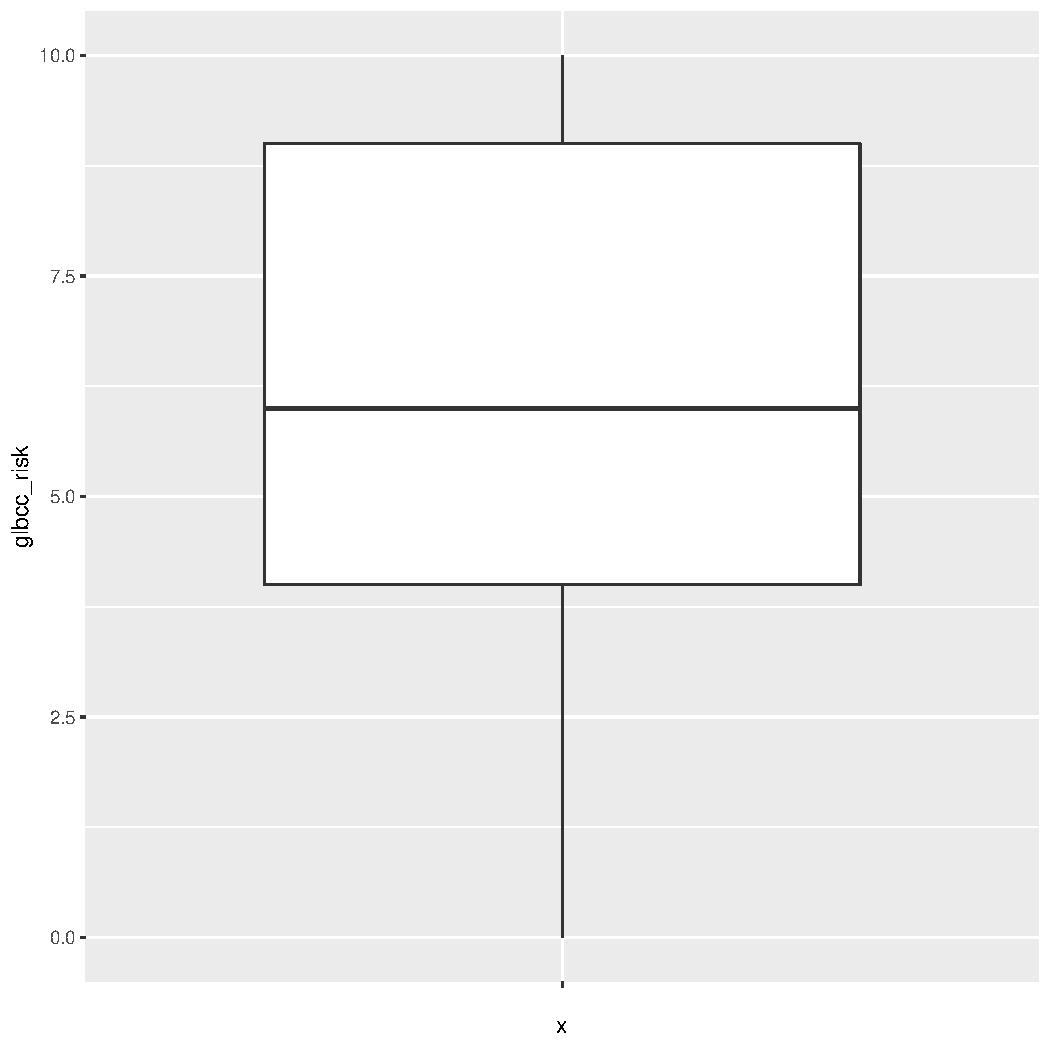
\includegraphics[width=4in]{03_Data/gccrskbox.pdf}%filname
\caption{Box-plot of Climate Change Risk 
\label{fig:boxrsk}}
\end{figure} 

\subsubsection{Percentiles}

\textit{Percentiles} list the data in hundredths. For example, scoring in the 99th percentile on the GRE means that 99\% of the other test takers
had a lower score. Percentiles can be incorporated with quartiles (and/or other order statistics) such that:
\begin{itemize}
\item First Quartile: 25th percentile 
\item Second Quartile: 50th percentile (the median) 
\item Third Quartile: 75th percentile 
\end{itemize}

Another way to compare a variable distribution to a theoretical distribution is with a quantile-comparison plot (qq plot). A qq plot displays the observed percentiles against those that would be expected in a normal distribution. This plot is often useful for examining the tails of the distribution, and deviations of a distribution from normality. This is shown in Figure \ref{fig:qqrsk}. 

\begin{knitrout}
\definecolor{shadecolor}{rgb}{0.969, 0.969, 0.969}\color{fgcolor}\begin{kframe}
\begin{alltt}
\hlkwd{ggplot}\hlstd{(ds,} \hlkwd{aes}\hlstd{(}\hlkwc{sample} \hlstd{= glbcc_risk))} \hlopt{+} \hlkwd{stat_qq}\hlstd{()}
\hlkwd{dev.off}\hlstd{()}
\end{alltt}
\end{kframe}
\end{knitrout}

\begin{figure}[!htp]
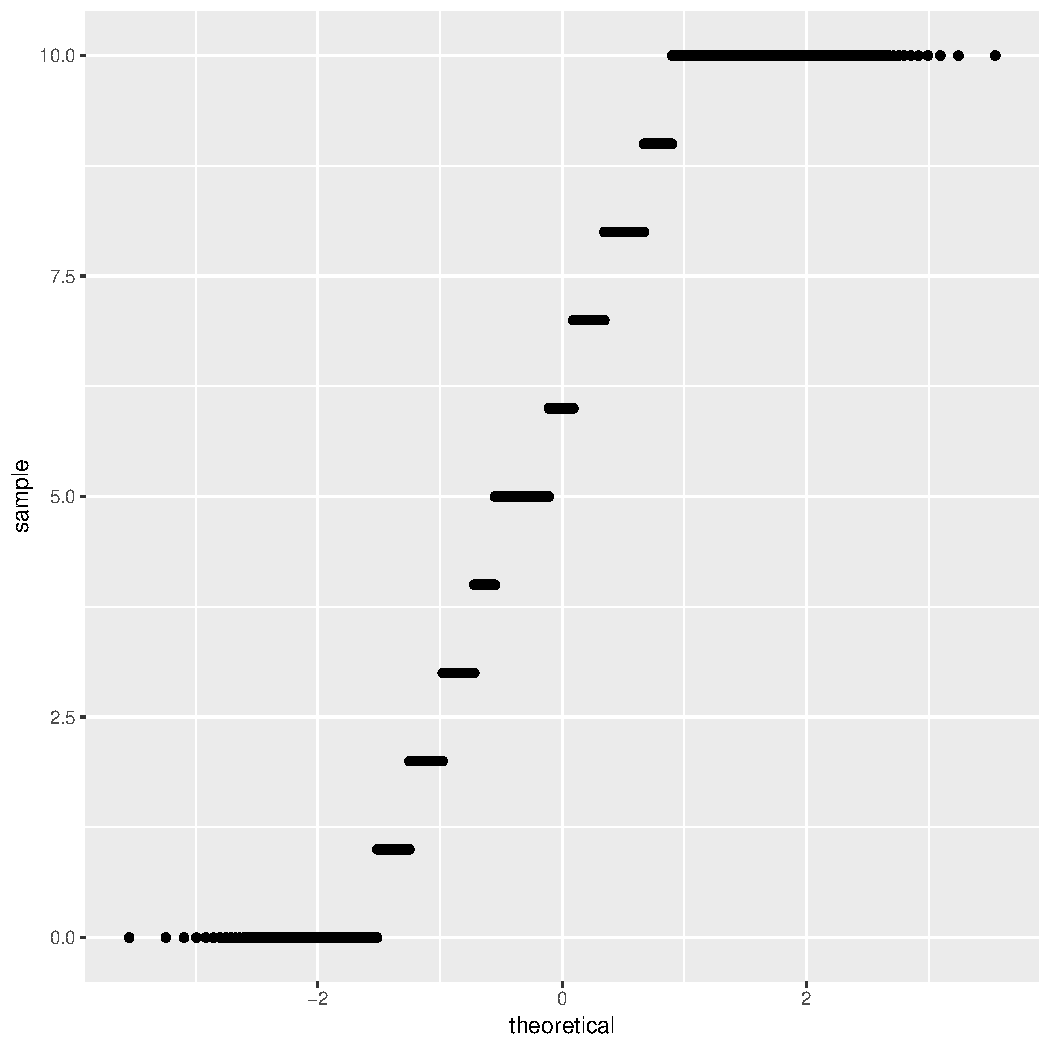
\includegraphics[width=4in]{03_Data/gccrskqq.pdf}%filename
\caption{QQ Plot of Climate Change Risk 
\label{fig:qqrsk}}
\end{figure}    

The qq plot provides an easy way to observe departures of a distribution from normality. For example, the plot shown in Figure \ref{fig:qqrsk} indicates the perceived risk measure has more observations in the tails of the distribution than would be expected if the variable was normally distributed.

\texttt{R} provides several ways to examine the central tendency, moments, and order statistics for variables and for entire data sets.  The \texttt{summary} function produces the minimum value, the first quartile, median, mean, third quartile, max value, and the number of missing values (Na's).

\begin{knitrout}
\definecolor{shadecolor}{rgb}{0.969, 0.969, 0.969}\color{fgcolor}\begin{kframe}
\begin{alltt}
\hlkwd{summary}\hlstd{(ds}\hlopt{$}\hlstd{ideol,} \hlkwc{na.rm} \hlstd{=} \hlnum{TRUE}\hlstd{)}
\end{alltt}
\begin{verbatim}
##    Min. 1st Qu.  Median    Mean 3rd Qu.    Max.    NA's 
##   1.000   4.000   5.000   4.653   6.000   7.000      23
\end{verbatim}
\begin{alltt}
\hlkwd{summary}\hlstd{(ds}\hlopt{$}\hlstd{age,} \hlkwc{na.rm} \hlstd{=} \hlnum{TRUE}\hlstd{)}
\end{alltt}
\begin{verbatim}
##    Min. 1st Qu.  Median    Mean 3rd Qu.    Max. 
##   18.00   52.00   62.00   60.37   70.00   99.00
\end{verbatim}
\begin{alltt}
\hlkwd{summary}\hlstd{(ds}\hlopt{$}\hlstd{gcclb_risk,} \hlkwc{na.rm} \hlstd{=} \hlnum{TRUE}\hlstd{)}
\end{alltt}
\begin{verbatim}
## Length  Class   Mode 
##      0   NULL   NULL
\end{verbatim}
\end{kframe}
\end{knitrout}
 
We can also use the \texttt{describe} function in the \texttt{psych} package to obtain more descriptive statistics, including skewness and
kurtosis. 

\begin{knitrout}
\definecolor{shadecolor}{rgb}{0.969, 0.969, 0.969}\color{fgcolor}\begin{kframe}
\begin{alltt}
\hlkwd{library}\hlstd{(psych)}
\hlkwd{describe}\hlstd{(ds}\hlopt{$}\hlstd{ideol)}
\end{alltt}
\begin{verbatim}
##    vars    n mean   sd median trimmed  mad min max range  skew kurtosis
## X1    1 2524 4.65 1.73      5    4.75 1.48   1   7     6 -0.45     -0.8
##      se
## X1 0.03
\end{verbatim}
\end{kframe}
\end{knitrout}
 
\subsection{Summary}
 
It is a serious mistake to get into your data analysis without understanding the basics of your data.  Knowing their range, the general distribution of your data, the shape of that distribution, their central tendency, and so forth will give you important clues as you move through your analysis and interpretation and prevent serious errors from occurring.  Readers also often need to know this information to provide a critical review of your work. 
 
Overall, this chapter has focused on understanding and characterizing data. We refer to the early process of evaluating a data set as rolling in the data -- getting to know the characteristic shapes of the distributions of each of the variables, the meanings of the scales, and the quality of the observations.  The discussion of central tendency, moments, and order statistics are all tools that you can use for that purpose. As a practicing scholar, policy analyst or public administration practitioner, this early stage in quantitative analysis is not optional; a failure to carefully and thoroughly understand your data can result in analytical disaster, excruciating embarrassment, and maybe even horrible encounters with the Killer Rabbit of Caerbannog. 
 
Think of rolling in the data, then, as your version of the Holy Hand Grenade of Antioch.




\chapter{Probability}

\textbf{Probability} tells us how likely something is to occur.  Probability concepts are also central to inferential statistics - something we will turn to shortly. Probabilities range from 0 (when there is no chance of the event occurring) to 1.0 (when the event will occur with certainty).  If you have a probability outside the 0 - 1.0 range, you have made an error!  Colloquially we often interchange probabilities and percentages, but probabilities refer to single events while percentages refer to the portion of repeated events that we get the outcome we are interested in.  As of this writing, Victor Martinez is hitting .329 which means each time he comes to bat he has a .329 probability of getting a hit or, 32.9\% of the times that he bats he gets a hit.  We symbolize probabilities as the P(A), where A is that Victor Martinez gets a hit.   Of course the probability that the event will not occur is 1 - P(A).

\section{Finding Probabilities}

There are two basic ways to find \textbf{simple probabilities}.  One way to find a probability is \textit{a priori}, or using logic without any real world evidence or experience.  If we know a die is not loaded, we know the probability of rolling a two is 1 out of 6 or .167.  Probabilities are easy to find if every possible outcome has the same probability of occurring.  If that is the case, the probability is number of ways your outcome can be achieved over all possible outcomes.  

The second method to determine a probability is called \textit{posterior}, which uses the experience and evidence that has accumulated over time to determine the likelihood of an event.  If we do not know that the probability of getting a head is the same as the probability of getting a tail when we flip a coin (and, therefore, we cannot use an a priori methodology), we can flip the coin repeatedly.  After flipping the coin, say, 6000 times, if we get 3000 heads you can conclude the probability of getting a head is .5, i.e., 3000 divided by 6000.
  
Sometimes we want to look at probabilities in a more complex way.  Suppose we want to know how Martinez fares against right-handed pitchers.  That kind of probability is referred to as a \textbf{conditional probability}.  The formal way that we might word that interest is: what is Martinez's probability of getting a hit given that the pitcher is right-handed?  We are establishing a condition (right-handed pitcher) and are only interested in the cases that satisfy the condition.  The calculation is the same as a simple probability, but it eliminates his at-bats against lefties and only considers those at bats against right-handed pitchers.   In this case, he has 23 hits in 56 at bats (against right-handed pitchers) so his probability of getting a hit against a right-handed pitcher is $23/56$ or .411.  (This example uses the posterior method to find the probability, by the way.)  A conditional probability is symbolized as $P(A|B)$ where A is getting a hit and B is the pitcher is right-handed.  It is read as the probability of A given B or the probability that Martinez will get a hit given that the pitcher is right-handed.

Another type of probability that we often want is a joint probability.  A \textbf{joint probability} tells the likelihood of two (or more) events both occurring.   Suppose you want to know the probability that you will like this course and that you will get an A in it, simultaneously -- the best of all possible worlds.   The formula for finding a joint probability is:

\begin{equation}
  \label{eq_label1}
  P(A \cap B) = P(A) * P(B|A) or P(B) * P(A|B)
\end{equation}

The probability of two events occurring at the same time is the probability that the first one will occur times the probability the second one will occur given that the first one has occurred.  

If events are independent the calculation is even easier.  Events are independent if the occurrence or non-occurrence of one does not affect whether the other occurs.  Suppose you want to know the probability of liking this course and not needing to get gas on the way home (your definition of a perfect day).  Those events are presumably independent so the $P(B|A) = P(B)$ and the joint formula for independent events becomes:

%need to convert this to other style equation
\begin{equation}
  \label{eq_label2}
  P(A \cap B) = P(A) * P(B)
\end{equation}

The final type of probability is the union of two probabilities.  The \textbf{union of two probabilities} is the probability that either one event will occur or the other will occur -- either, or, it does not matter which one.  You might go into a statistics class with some dread and you might say a little prayer to yourself: ``Please let me either like this class or get an A.  I do not care which one, but please give me at least one of them."  The formula and symbols for that kind of probability is:

\begin{equation}
  \label{eq_label3}
  P(A \cup B) = P(A) + P(B) - P(A \cap B)
\end{equation}

It is easy to understand why we just add the $P(A)$ and the $P(B)$ but it may be less clear why we subtract the joint probability.   The answer is simple - because we counted where they overlap twice (those instances in both A and in B) so we have to subtract out one instance.  

If, though, the events are mutually exclusive, we do not need to subtract the overlap.  Mutually exclusive events are events that cannot occur at the same time, so there is no overlap.  Suppose you are from Chicago and will be happy if either the Cubs or the White Sox win the World Series.  Those events are mutually exclusive since only one team can win the World Series so to find the union of those probabilities we simple have to add the probability of the Cubs winning to the probability of the White Sox winning.

\section{Finding Probabilities with the Normal Curve}
If we want to find the probability of a score falling in a certain range, e.g., between 3 and 7, or more than 12, we can use the normal to determine that probability.  Our ability to make that determination is based on some known characteristics on the normal curve.  We know that for all normal curves 68.26\% of all scores fall within one standard deviation of the mean, that 95.44\% fall within two standard deviations, and that 99.72\% fall within three standard deviations.  (The normal distribution is dealt with more formally in the next chapter.) So, we know that something that is three or more standard deviations above the mean is pretty rare.  Figure \ref{fig_normalcurve} illustrates the probabilities associated with the normal curve.

\begin{figure}
  \centering
  \includegraphics[width=1.0\textwidth]%
    {04_Probability/Graphics/Normal_curve_probability.jpg}% picture filename
  \caption{Area under the Normal Curve \\ source - \url{http://whatilearned.wikia.com/wiki/File:Normal_curve_probability.jpg} \label{fig_normalcurve}}
\end{figure}

According to Figure \ref{fig_normalcurve}, there is a .3413 probability of an observation falling between the mean and one standard deviation above the mean and, therefore, a .6826 probability of a score falling within $(+/-)$ one standard deviation of the mean.   There is also a .8413 probability of a score being one standard deviation above the mean or less (.5 probability of a score falling below the mean and a .3413 probability of a score falling between the mean and one standard deviation above it).   (Using the language we learned in Chapter 3, another way to articulate that finding is to say that a score one standard deviation above the mean is at the 84th percentile.)  There is also a .1587 probability of a score being a standard deviation above the mean or higher $(1.0 - .8413)$. 

Intelligence tests have a mean of 100 and a standard deviation of 15.  Someone with an IQ of 130, then, is two standard deviations above the mean, meaning they score higher than 97.72\% of the population.  Suppose, though, your IQ is 140.  Using Figure \ref{fig_normalcurve} would enable us only to approximate how high that score is.  To find out more precisely, we have to find out how many standard deviations above the mean 140 is and then go to a more precise normal curve table.

To find out how many standard deviations from the mean an observation is, we calculated a standardized, or \textbf{Z-score}.  The formula to convert a raw score to a Z-score is:

\begin{equation}
  \label{eq_label4}
Z = \frac{x-\mu}{\sigma}
\end{equation}

In this case, the $Z$-score is $140-100/15$ or $2.67$.  Looking at the formula, you can see that a Z-score of zero puts that score at the mean; a $Z$-score of one is one standard deviation above the mean; and a $Z$-score of $2.67$ is $2.67$ standard deviations above the mean.

The next step is to go to a normal curve table to interpret that Z-score.  Table \ref{tab_Normal_Curve} at the end of the chapter contains such a table.  To use the table you combine rows and columns to find the score of 2.67.  Where they cross we see the value .4962.  That value means there is a .4962 probability of scoring between the mean and a $Z$-score of 2.67.  Since there is a .5 probability of scoring below the mean adding the two values together gives a .9962 probability of finding an IQ of 140 or lower or a .0038 probability of someone having an IQ of 140 or better.

\begin{grbox}
  \greybox{\textbf{Bernoulli Probabilities}\\
We can use a calculation known as the Bernoulli Process to determine the probability of a certain number of successes in a given number of trials.  For example, if you want to know the probability of getting exactly three heads when you flip a coin four times, you can use the Bernoulli calculation.  To perform the calculation you need to determine the number of trials $(n)$, the number of successes you care about $(k)$, the probability of success on a single trial $(p)$, and the probability $(q)$ of not a success $(1-p$ or $q)$.  The operative formula is:

\begin{equation}
 \label{eq_label5}
 \left(\frac{n!}{k!(n-k)!}\right) * p^k * q^{n-k}
\end{equation}

The symbol $n!$ is ``n factorial" or $n*(n-1)*(n-2)$ ... $* 1$.  So if you want to know the probability of getting three heads on four flips of a coin, $n=4$, $k=3$, $p=.5$, and $q=.5$:

\begin{equation}
  \label{eq_label6}
  \left(\frac{4!}{3!(4-3)!}\right) * .5^3 * .5^{4-3} = .25
\end{equation}

The Bernoulli process can be used only when both $n * p$ and $n * q$ are greater than ten.  It is also most useful when you are interested in exactly $k$ successes.  If you want to know the probability of $k$ or more, or $k$ or fewer successes, it is easier to use the normal curve.  Bernoulli could still be used if your data is discrete, but you would have to do repeated calculations.
}
\end{grbox}

\section{Summary}
Probabilities are simple statistics but are important when we want to know the likelihood of some event occurring.  There are frequent real world instances where we find that information valuable.  We will see, starting in the next chapter, that probabilities are also central to the concept of inference.

\newpage
\textbf{Appendix 4.1 The Normal Curve Table}

\begin{table}[h]
\caption{Standard Normal Distribution - Area under the Normal Curve from 0 to X}
\label{tab_Normal_Curve}
\resizebox{\textwidth}{!}{%
\begin{tabular}{lcccccccccc}
\hline
\multicolumn{1}{l}{z} & \multicolumn{1}{c}{0.00} & \multicolumn{1}{c}{0.01} & \multicolumn{1}{c}{0.02} & \multicolumn{1}{c}{0.03} & \multicolumn{1}{c}{0.04} & \multicolumn{1}{c}{0.05} & \multicolumn{1}{c}{0.06} & \multicolumn{1}{c}{0.07} & \multicolumn{1}{c}{0.08} & \multicolumn{1}{c}{0.09} \\ \hline
0.0 & 0.00000 & 0.00399 & 0.00798 & 0.01197 & 0.01595 & 0.01994 & 0.02392 & 0.02790 & 0.03188 & 0.03586 \\
0.1 & 0.0398 & 0.04380 & 0.04776 & 0.05172 & 0.05567 & 0.05966 & 0.0636 & 0.06749 & 0.07142 & 0.07535 \\
0.2 & 0.0793 & 0.08317 & 0.08706 & 0.09095 & 0.09483 & 0.09871 & 0.10257 & 0.10642 & 0.11026 & 0.11409 \\
0.3 & 0.11791 & 0.12172 & 0.12552 & 0.12930 & 0.13307 & 0.13683 & 0.14058 & 0.14431 & 0.14803 & 0.15173 \\
0.4 & 0.15542 & 0.15910 & 0.16276 & 0.16640 & 0.17003 & 0.17364 & 0.17724 & 0.18082 & 0.18439 & 0.18793 \\
0.5 & 0.19146 & 0.19497 & 0.19847 & 0.20194 & 0.20540 & 0.20884 & 0.21226 & 0.21566 & 0.21904 & 0.22240 \\
0.6 & 0.22575 & 0.22907 & 0.23237 & 0.23565 & 0.23891 & 0.24215 & 0.24537 & 0.24857 & 0.25175 & 0.25490 \\
0.7 & 0.25804 & 0.26115 & 0.26424 & 0.26730 & 0.27035 & 0.27337 & 0.27637 & 0.27935 & 0.28230 & 0.28524 \\
0.8 & 0.28814 & 0.29103 & 0.29389 & 0.29673 & 0.29955 & 0.30234 & 0.30511 & 0.30785 & 0.31057 & 0.31327 \\
0.9 & 0.31594 & 0.31859 & 0.32121 & 0.32381 & 0.32639 & 0.32894 & 0.33147 & 0.33398 & 0.33646 & 0.33891 \\
1.0 & 0.34134 & 0.34375 & 0.34614 & 0.34849 & 0.35083 & 0.35314 & 0.35543 & 0.35769 & 0.35993 & 0.36214 \\
1.1 & 0.36433 & 0.36650 & 0.36864 & 0.37076 & 0.37286 & 0.37493 & 0.37698 & 0.37900 & 0.38100 & 0.38298 \\
1.2 & 0.38493 & 0.38686 & 0.38877 & 0.39065 & 0.39251 & 0.39435 & 0.39617 & 0.39796 & 0.39973 & 0.40147 \\
1.3 & 0.40320 & 0.40490 & 0.40658 & 0.40824 & 0.40988 & 0.41149 & 0.41308 & 0.41466 & 0.41621 & 0.41774 \\
1.4 & 0.41924 & 0.42073 & 0.42220 & 0.42364 & 0.42507 & 0.42647 & 0.42785 & 0.42922 & 0.43056 & 0.43189 \\
1.5 & 0.43319 & 0.43448 & 0.43574 & 0.43699 & 0.43822 & 0.43943 & 0.44062 & 0.44179 & 0.44295 & 0.44408 \\
1.6 & 0.44520 & 0.44630 & 0.44738 & 0.44845 & 0.44950 & 0.45053 & 0.45154 & 0.45254 & 0.45352 & 0.45449 \\
1.7 & 0.45543 & 0.45637 & 0.45728 & 0.45818 & 0.45907 & 0.45994 & 0.46080 & 0.46164 & 0.46246 & 0.46327 \\
1.8 & 0.46407 & 0.46485 & 0.46562 & 0.46638 & 0.46712 & 0.46784 & 0.46856 & 0.46926 & 0.46995 & 0.47062 \\
1.9 & 0.47128 & 0.47193 & 0.47257 & 0.47320 & 0.47381 & 0.47441 & 0.47500 & 0.47558 & 0.47615 & 0.47670 \\
2.0 & 0.47725 & 0.47778 & 0.47831 & 0.47882 & 0.47932 & 0.47982 & 0.48030 & 0.48077 & 0.48124 & 0.48169 \\
2.1 & 0.48214 & 0.48257 & 0.48300 & 0.48341 & 0.48382 & 0.48422 & 0.48461 & 0.48500 & 0.48537 & 0.48574 \\
2.2 & 0.48610 & 0.48645 & 0.48679 & 0.48713 & 0.48745 & 0.48778 & 0.48809 & 0.48840 & 0.48870 & 0.48899 \\
2.3 & 0.48928 & 0.48956 & 0.48983 & 0.49010 & 0.49036 & 0.49061 & 0.49086 & 0.49111 & 0.49134 & 0.49158 \\
2.4 & 0.49180 & 0.49202 & 0.49224 & 0.49245 & 0.49266 & 0.49286 & 0.49305 & 0.49324 & 0.49343 & 0.49361 \\
2.5 & 0.49379 & 0.49396 & 0.49413 & 0.49430 & 0.49446 & 0.49461 & 0.49477 & 0.49492 & 0.49506 & 0.49520 \\
2.6 & 0.49534 & 0.49547 & 0.49560 & 0.49573 & 0.49585 & 0.49598 & 0.49609 & 0.49621 & 0.49632 & 0.49643 \\
2.7 & 0.49653 & 0.49664 & 0.49674 & 0.49683 & 0.49693 & 0.49702 & 0.49711 & 0.49720 & 0.49728 & 0.49736 \\
2.8 & 0.49744 & 0.49752 & 0.49760 & 0.49767 & 0.49774 & 0.49781 & 0.49788 & 0.49795 & 0.49801 & 0.49807 \\
2.9 & 0.49813 & 0.49819 & 0.49825 & 0.49831 & 0.49836 & 0.49841 & 0.49846 & 0.49851 & 0.49856 & 0.49861 \\
3.0 & 0.49865 & 0.49869 & 0.49874 & 0.49878 & 0.49882 & 0.49886 & 0.49889 & 0.49893 & 0.49896 & 0.49900 \\ 
4.0 & 0.49979 & \multicolumn{1}{l}{} & \multicolumn{1}{l}{} & \multicolumn{1}{l}{} & \multicolumn{1}{l}{} & \multicolumn{1}{l}{} & \multicolumn{1}{l}{} & \multicolumn{1}{l}{} & \multicolumn{1}{l}{} & \multicolumn{1}{l}{}  \\
5.0 & 0.4999997 & \multicolumn{1}{l}{} & \multicolumn{1}{l}{} & \multicolumn{1}{l}{} & \multicolumn{1}{l}{} & \multicolumn{1}{l}{} & \multicolumn{1}{l}{} & \multicolumn{1}{l}{} & \multicolumn{1}{l}{} & \multicolumn{1}{l}{} \\ \hline
\end{tabular}
}
\end{table}
\FloatBarrier




\chapter{Inference}


This chapter considers the role of inference---learning about populations from samples---and the practical and theoretical importance of understanding the characteristics of your data before attempting to undertake statistical analysis. As we noted in the prior chapters, it is a vital first step in empirical analysis to ``roll in the data."

\section{Inference: Populations and Samples}

The basis of hypothesis testing with statistical analysis is \textbf{inference}. In short, inference---and inferential statistics by extension---means deriving knowledge about a population from a sample of that population. Given that in most contexts it is not possible to have all the data on an entire population of interest, we therefore need to sample from that population.\footnote{It is important to keep in mind that, for purposes of theory building, the population of interest may not be finite. For example, if you theorize about general properties of human behavior, many of the members of the human population are not yet (or are no longer) alive. Hence it is not possible to include all of the population of interest in your research. We therefore rely on samples.} However, in order to be able to rely on inference, the sample must cover the theoretically relevant variables, variable ranges, and contexts. 

\subsection{Populations and Samples} 

In doing statistical analysis we differentiate between populations and samples.  The population is the total set of items that we care about.  The sample is a subset of those items that we study in order to understand the population.  While we are interested in the population we often need to resort to studying a sample due to time, financial, or logistic constraints that might make studying the entire population infeasible. Instead, we use inferential statistics to make inferences about the population from a sample.

\subsection{Sampling and Knowing} 

Take a relatively common -- but perhaps less commonly examined -- expression about what we ``know" about the world around us. We commonly say we ``know" people, and some we know better than others. What does it mean to know someone? In part it must mean that we can anticipate how that person would behave in a wide array of situations. If we know that person from experience, then it must be that we have observed their behavior across a 
sufficient variety of situations in the past to be able to infer how they would behave in  future situations. Put differently, we have ``sampled" their behavior across a relevant range of situations and contexts to be confident that we can anticipate their behavior in the future.\footnote{Of course, we also need to estimate changes -- both gradual and abrupt -- in how people behave over time, which is the province of time-series analysis.} Similar considerations about sampling might apply to ``knowing" a place, a group, or an institution. Of equal importance, samples of observations
across different combinations of variables are necessary to identify relationships (or functions) between variables.  In short, samples -- whether deliberately drawn and systematic or otherwise -- are integral to what we think we know of the world around us.

\subsection{Sampling Strategies} 

Given the importance of sampling, it should come as little surprise that there are numerous strategies designed to provide useful inference about populations. For example, how can we judge whether the temperature of a soup is appropriate before serving it? We might stir the pot, to assure uniformity of temperature across possible (spoon-sized) samples, then sample a spoonful. A particularly thorny problem in sampling concerns the practice of courtship, in which participants may attempt to put ``their best foot forward" to make a good impression. Put differently, the participants often seek to bias the sample of relational experiences to make themselves look better than they might on average. Sampling in this context usually involves (a) getting opinions of others, thereby broadening (if only indirectly) the size of the sample, and (b) observing the courtship partner over a wide range of circumstances in which the intended bias may be difficult to maintain. Put formally, we may try to stratify the sample by taking observations in appropriate ``cells" that correspond to different potential influences on behavior -- say, high stress environments involving preparation for final exams or meeting parents. In the best possible case, however, we try to wash out the effect of various influences on our samples through randomization. To pursue the courtship example (perhaps a bit too far!), observations of behavior could be taken across interactions from a randomly assigned array of partners and situations. But, of course, by then all bets are off on things working out anyway.

\subsection{Sampling Techniques}

When engaging in inferential statistics to infer about the characteristics a population from a sample, it is essential to be clear about how the sample was drawn. Sampling can be a very complex subject with multiple stages involved in drawing the final sample. It is desirable that the sample is some form of a \textbf{probability sample}, i.e., a sample in which each member of the population has a known probability of being sampled.   The most direct form of an appropriate probability sample is a \textbf{random sample} where everyone has the same probability of being sampled.  A random sample has the advantages of simplicity (in theory) and ease of inference as no adjustments to the data are needed.  But, the reality of conducting a random sample may make the process quite challenging.  Before we can draw subjects at random, we need a list of all members of the population.  For many populations (e.g. adult US residents) that list is impossible to get.  Not too long ago, it was reasonable to conclude that a list of telephone numbers was a reasonable approximation of such a listing for American households.  During the era that landlines were ubiquitous, pollsters could randomly call numbers (and perhaps ask for the adult in the household who had the most recent birthday) to get a good approximation of a national random sample.  (It was also an era before caller identification and specialized ringtones which meant that calls were routinely answered decreasing - but not eliminating - the concern with response bias.)  Of course, telephone habits have changed and pollsters finding it increasingly difficult to make the case that random dialing of landlines serves as a representative sample of adult Americans.

Other forms of probability sampling are frequently used to overcome some of the difficulties that pure random sampling presents.  Suppose our analysis will call upon us to make comparisons based on race.  Only 12.6\% of Americans are African-American.  Suppose we also want to take into account religious preference.  Only 5\% of African-Americans are Catholic, which means that only .6\% of the population is both.  If our sample size is 500, we might end up with three Catholic African-Americans.  A \textbf{stratified random sample} (also called a quota sample) can address that problem.  A stratified random sample is similar to a simple random sample, but will draw from different subpopulations, strata, at different rates.  The total sample needs to be weighted, then, to be representative of the entire population.
  
Another type of probability sample that is common in face-to-face surveys relies on \textbf{cluster sampling}.  Cluster sampling initially samples based on clusters (generally geographic units, such as census tracts) and then samples participants within those units.  In fact, this approach often uses multi-level sampling where the first level might be a sample of congressional districts, then census tracts, and then households.  The final sample will need to be weighted in a complex way to reflect varying probabilities that individuals will be included in the sample.  
  
\textbf{Non-probability samples}, or those for which the probability of inclusion of a member of the population in the sample is unknown, can raise difficult issues for statistical inference; however, under some conditions, they can be considered representative and used for inferential statistics.

\textbf{Convenience samples} (e.g., undergraduate students in the Psychology Department subject pool) are accessible and relatively low cost, but may differ from the larger population to which you want to infer in important respects.   Necessity may push a researcher to use a convenience sample, but inference should be approached with caution.  A convenience sample based on ``I asked people who come out of the bank" might provide quite different results from a sample based on ``I asked people who come out of a payday loan establishment".

Some non-probability samples are used because the researcher does not want to make inferences to a larger population.  A \textbf{purposive or judgmental sample} relies on the researcher's discretion regarding who can bring useful information to bear on the subject matter.  If we want to know why a piece of legislation was enacted, it makes sense to sample the author and co-authors of the bill, committee members, leadership, etc. rather than a random sample of members of the legislative body.

\textbf{Snowball sampling} is similar to a purposive sample in that we look for people with certain characteristics but rely on subjects to recommend others who meet the criteria we have in place.  We might want to know about struggling young artists.  They may be hard to find, though, since their works are not hanging in galleries so we may start with a one or more that we can find and then ask them who else we should interview.
	
Increasingly, various kinds of non-probability samples are employed in social science research, and when this is done it is critical that the potential biases associated with the samples be evaluated.  But there is also growing evidence that non-probability samples can be used inferentially - when done very carefully, using complex adjustments.  Wang, et al. (2014) demonstrate that a sample of Xbox users could be used to forecast the 2012 presidential election outcome. \footnote{Wei Wang, David Rothschild, Sharad Goel, and Andrew Gelman (2014)  ''Forecasting Elections with Non-Representative Polls," Preprint submitted to \textit{International Journal of Forecasting} March 31, 2014.}  The overview of the technique is relatively simple, but the execution is more challenging.  They divided their data into cells based on politically and demographically relevant variables (e.g., party id, gender, race, etc.) and ended up with over 175,000 cells - poststratification.  (There were about three-quarters of a million participants in the Xbox survey).  Basically, they found the vote intention within each cell and then weighted each cell based on a national survey using multilevel regression.   Their final results were strikingly accurate.   Similarly, Nate Silver with FiveThirtyEight, has demonstrated remarkable ability to forecast based on his weighted sample of polls taken by others.
  
Sampling techniques can be relatively straightforward, but as one moves away from simple random sampling, the sampling process either becomes more complex or limits our ability to draw inferences about a population.  Researchers use all of these techniques for good purposes and the best technique will depend on a variety of factors, such as budget, expertise, need for precision, and what research question is being addressed. For the remainder of this text, though, when we talk about drawing inferences, the data will based upon an appropriately drawn, probability sample.

%%%This is from the first edition for reference.
\subsection{So How is it That We Know?} 

So why is it that the characteristics of samples can tell us a lot about the characteristics of populations? If samples are properly drawn, the observations taken will provide a range of values on the measures of interest that reflect those of the larger population. The connection is that we expect the phenomenon we are measuring will have a \textbf{distribution} within the population, and a sample of observations drawn from the population will provide useful information about that distribution. The theoretical connection comes from probability theory, which concerns the analysis of random phenomena. For present purposes, if we randomly draw a sample of observations on a measure for an individual (say, discrete acts of kindness), we can use probability theory to make inferences about the characteristics of the overall population of the phenomenon in question. More specifically, probability theory allows us to make inference about the shape of that distribution -- how frequent are acts of kindness committed, or what proportion of acts evidence kindness?

In sum, samples provide information about  \textbf{probability distributions}. Probability distributions include all possible values and the probabilities associated with those values. The \textbf{normal distribution} is the key probability distribution in inferential statistics.

\section{The Normal Distribution} 

For purposes of statistical inference, the normal distribution is one of the most important types of probability distributions. It forms the basis of many of the assumptions needed to do quantitative data analysis, and is the basis for a wide range of hypothesis tests.  A standardized normal distribution has a mean, $\mu$, of $0$ and a standard deviation (s.d.), $\sigma$, of $1$. The distribution of an outcome variable, $Y$, can be
described: 

\begin{equation}
  \label{eq:norm}
  Y \sim N(\mu_Y,\sigma^{2}_Y)
\end{equation}

\noindent where $\sim$ stands for ``distributed as'', $N$ indicates the normal distribution, and mean $\mu_Y$ and variance $\sigma^{2}_Y$ are
the parameters. The probability function of the normal distribution is expressed below:

\begin{description}
  \item [The Normal Probability Density Function] The probability density function (PDF) of a normal
    distribution with mean $\mu$ and 
      standard deviation $\sigma$: 
      \begin{center}
        $f(x) = \frac{1}{\sigma \sqrt{2 \pi}} e^{-(x-\mu)^{2}/2\sigma^{2}}$
      \end{center}
  \item [The Standard Normal Probability Density Function] The
    standard normal PDF has a $\mu=0$ and $\sigma=1$
      \begin{center}
        $f(x) = \frac{1}{\sqrt{2 \pi}}e^{-x^{2}/2}$
      \end{center}     
\end{description}
Using the standard normal PDF, we can plot a normal distribution in
\texttt{R}.  
\begin{knitrout}
\definecolor{shadecolor}{rgb}{0.969, 0.969, 0.969}\color{fgcolor}\begin{kframe}
\begin{alltt}
\hlstd{x} \hlkwb{<-} \hlkwd{seq}\hlstd{(}\hlopt{-}\hlnum{4}\hlstd{,} \hlnum{4}\hlstd{,} \hlkwc{length} \hlstd{=} \hlnum{200}\hlstd{)}
\hlstd{y} \hlkwb{<-} \hlnum{1}\hlopt{/}\hlkwd{sqrt}\hlstd{(}\hlnum{2} \hlopt{*} \hlstd{pi)} \hlopt{*} \hlkwd{exp}\hlstd{(}\hlopt{-}\hlstd{x}\hlopt{^}\hlnum{2}\hlopt{/}\hlnum{2}\hlstd{)}
\hlkwd{plot}\hlstd{(x, y,} \hlkwc{type} \hlstd{=} \hlstr{"l"}\hlstd{,} \hlkwc{lwd} \hlstd{=} \hlnum{2}\hlstd{)}
\end{alltt}
\end{kframe}
\end{knitrout}
\begin{figure}
  \centering
  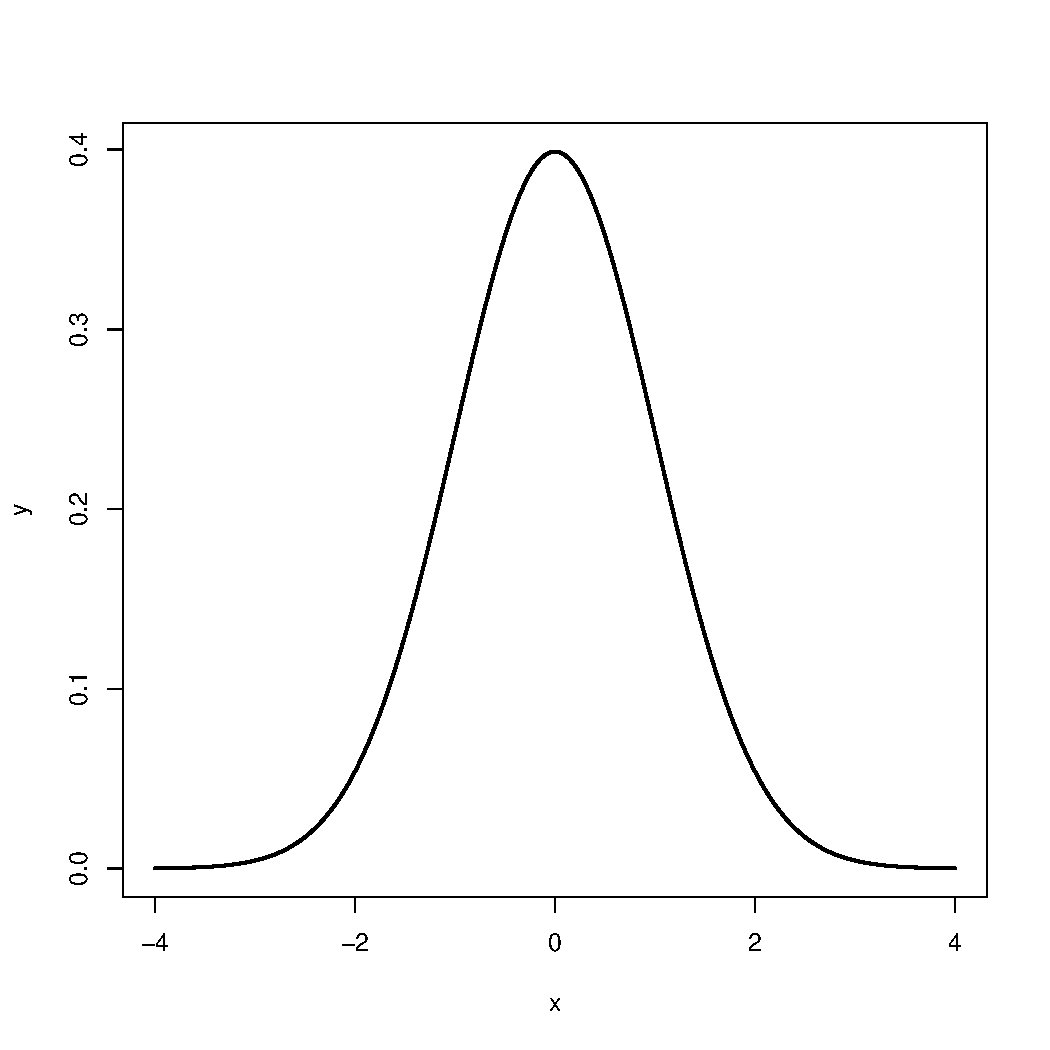
\includegraphics[width=4in]{05_Inference/normal.pdf}% picture filename
  \caption[Normal Distribution]{The Normal Distribution  \label{normal}}
\end{figure}
\noindent Note that the the tails go to $\pm \infty$. In addition, the density of a distribution over the range of x is the key to hypothesis testing With a normal distribution, $\sim68\%$ of the observations will fall within $1$ standard deviation of the mean, $\sim 95\%$ will fall within 2 standard deviations, and $\sim 99.7\%$ within 3 standard deviations. This is illustrated in Figure \ref{fig:norm}. 





\begin{figure}
        \centering
        \begin{subfigure}[b]{0.4\textwidth}
                \centering
                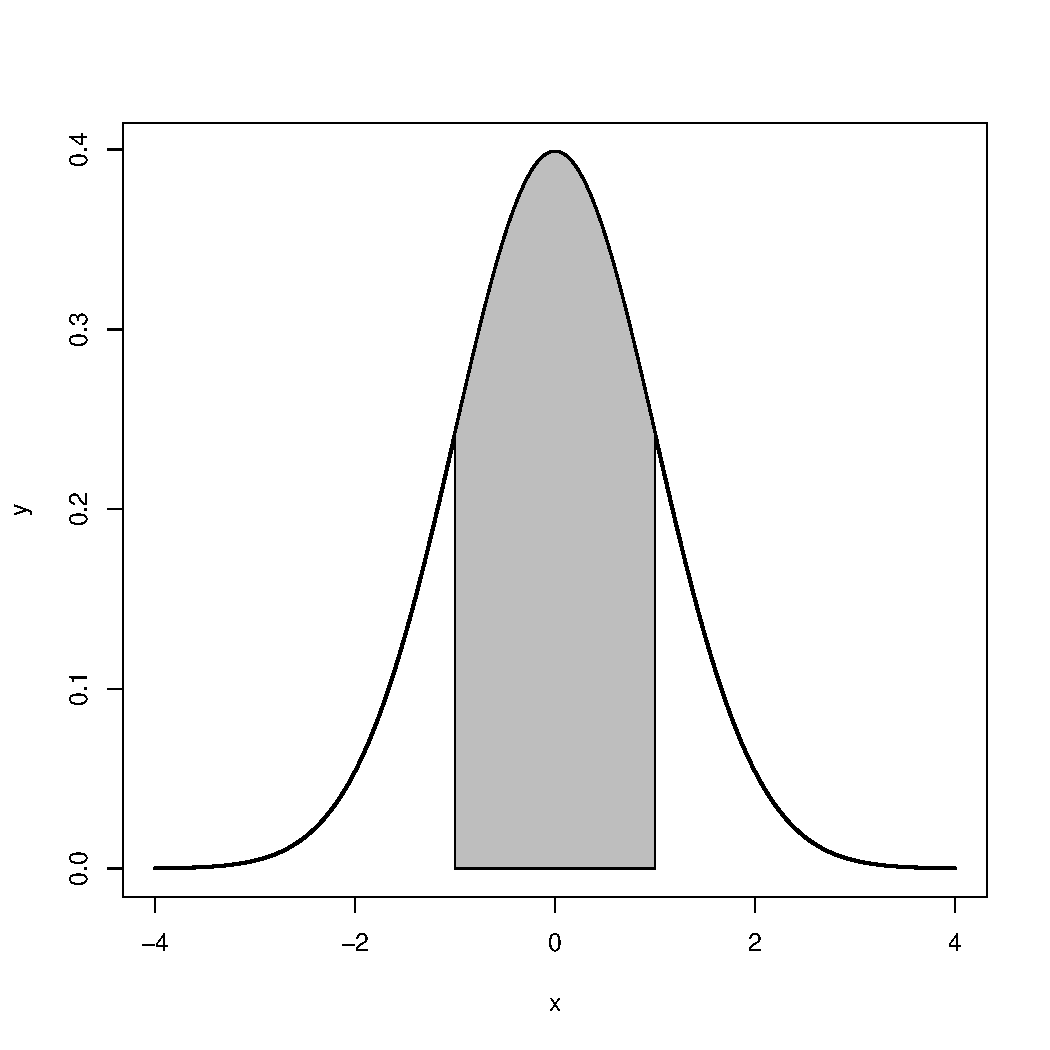
\includegraphics[width=\textwidth]{05_Inference/normal68.pdf}
                \caption{$\sim 68\%$: 1 s.d. \label{fig:norm68}}
        \end{subfigure}
        \begin{subfigure}[b]{0.4\textwidth}
                \centering
                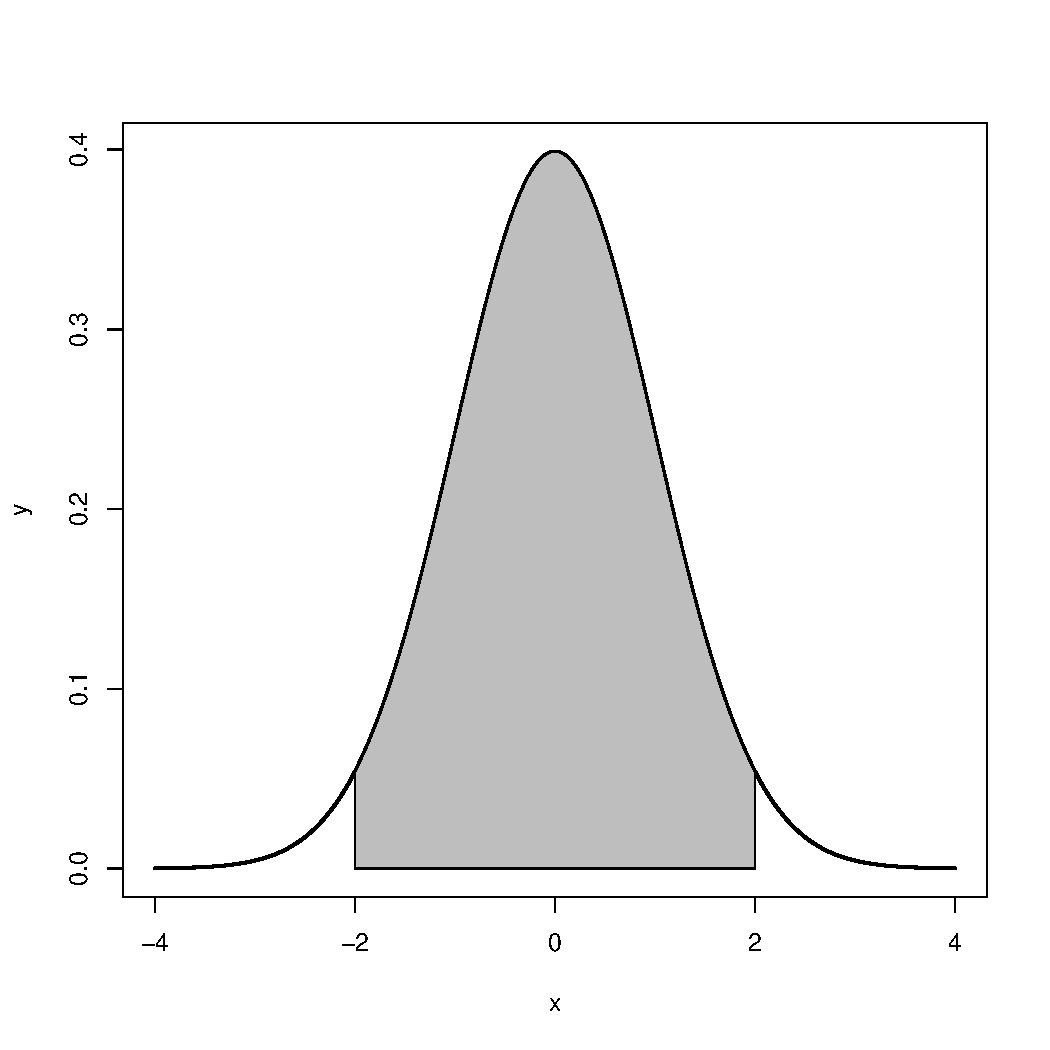
\includegraphics[width=\textwidth]{05_Inference/normal95.pdf}
                \caption{$\sim 95\%$: 2 s.d.  \label{fig:norm95}}
        \end{subfigure}
        \begin{subfigure}[b]{0.4\textwidth}
                \centering
                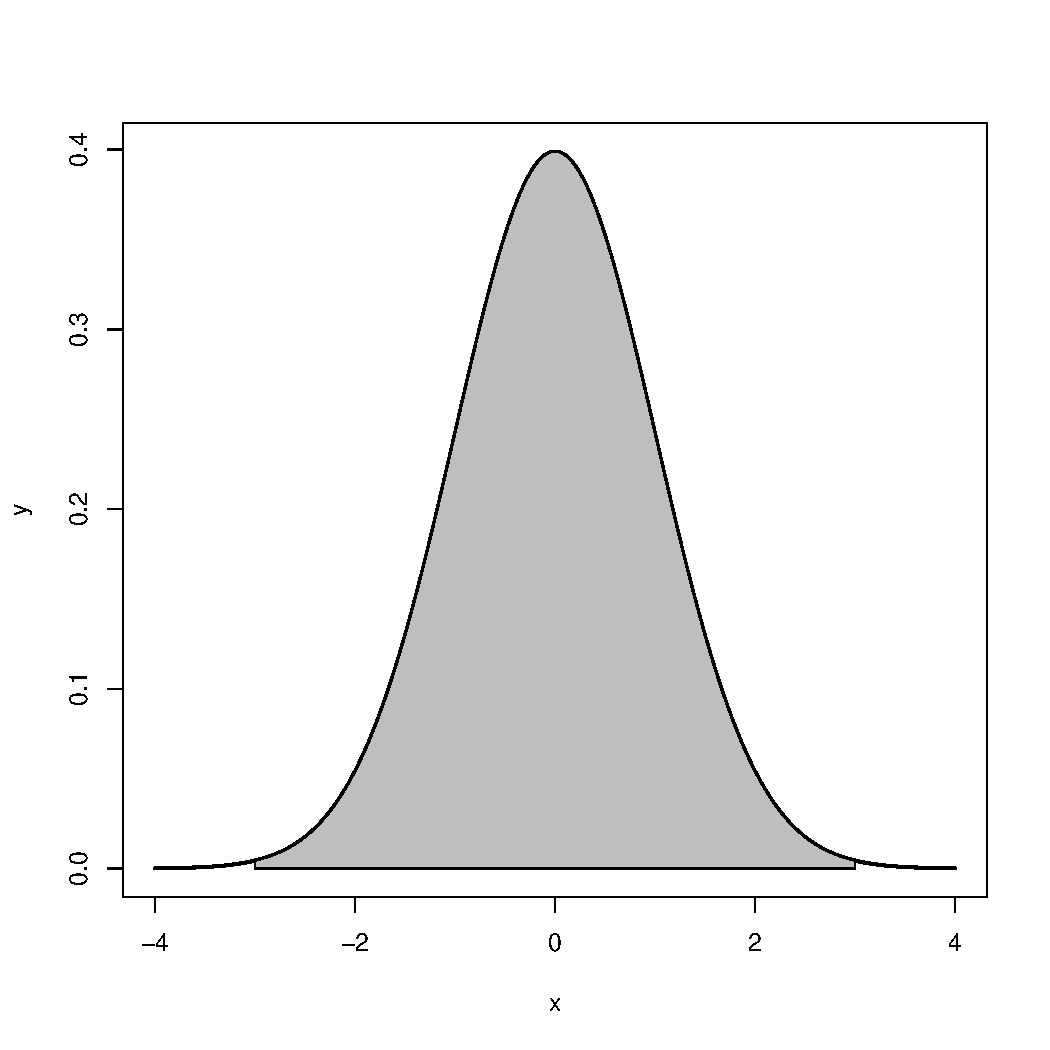
\includegraphics[width=\textwidth]{05_Inference/normal99.pdf}
                \caption{$\sim 99.7\%$: 3 s.d. \label{fig:norm99}}
        \end{subfigure}
        \caption{Normal Distribution and Standard Deviations \label{fig:norm}}
\end{figure}

The normal distribution is characterized by several important properties. The distribution of observations is symmetrical around the mean $\mu$; the frequency of observations is highest (the mode) at $\mu$, with more extreme values occurring with lower frequency (this can be seen in Figure \ref{fig:norm}); and only the mean and variance are needed to characterize data and test simple hypotheses. 

\begin{grbox}
  \greybox{\textbf{The Properties of the Normal Distribution}
    \begin{itemize}
    \item It is symmetrical around its mean and median, $\mu$
    \item The highest probability (aka "the mode") occurs at its mean value 
    \item Extreme values occur in the tails 
    \item It is fully described by its two parameters, $\mu$ and $\sigma^{2}$  
    \end{itemize}}
\end{grbox}

If the values for $\mu$ and $\sigma^{2}$ are known, which might be the case with a population, then we can calculate a $Z$-score to compare differences in $\mu$ and $\sigma^{2}$ between two normal distributions or obtain the probability for a given value given $\mu$ and $\sigma^{2}$. The $Z$-score is calculated: 
\begin{equation}
  \label{eq:z}
  Z = \frac{Y-\mu_Y}{\sigma}
\end{equation} 

Therefore, if we have a normal distribution with a $\mu$ of 70 and a $\sigma^{2}$ of 9, we can calculate a probability for $i=75$. First we
calculate the $Z$-score, then we determine the probability of that score based on the normal distribution. 
\begin{knitrout}
\definecolor{shadecolor}{rgb}{0.969, 0.969, 0.969}\color{fgcolor}\begin{kframe}
\begin{alltt}
\hlstd{z} \hlkwb{<-} \hlstd{(}\hlnum{75} \hlopt{-} \hlnum{70}\hlstd{)}\hlopt{/}\hlnum{3}
\hlstd{z}
\end{alltt}
\begin{verbatim}
## [1] 1.666667
\end{verbatim}
\begin{alltt}
\hlstd{p} \hlkwb{<-} \hlkwd{pnorm}\hlstd{(}\hlnum{1.67}\hlstd{)}
\hlstd{p}
\end{alltt}
\begin{verbatim}
## [1] 0.9525403
\end{verbatim}
\begin{alltt}
\hlstd{p} \hlkwb{<-} \hlnum{1} \hlopt{-} \hlstd{p}
\hlstd{p}
\end{alltt}
\begin{verbatim}
## [1] 0.04745968
\end{verbatim}
\end{kframe}
\end{knitrout}

\noindent As shown, a score of $75$ falls just outside two standard deviations ($>0.95$), and the probability of obtaining that score when $\mu = 70$ and $\sigma^{2} = 9$ is just under 5\%.  

\subsection{Standardizing a Normal Distribution and Z-scores}

A distribution can be plotted using the raw scores found in the original data.  That plot will have a mean and standard  deviation calculated from the original data. To utilize the normal curve to determine probability functions and for inferential statistics we will want to convert that data so that it is standardized.  We standardize so that the distribution is consistent across all distributions.  That standardization produces a set of scores that have a mean of zero and a standard deviation of one.   A standardized or Z-score of 1.5 means, therefore, that the score is one and a half standard deviations about the mean.  A Z-score of -2.0 means that the score is two standard deviations below the mean.

As formula 4.4 indicates, standardizing is a simple process.  To move the mean from its original value to a mean of zero, all you have to do is subtract the mean from each score.  To standardize the standard deviation to one all that is necessary is to divide each score the standard deviation.

% note the above should be changed to a label. - the label is eq_label4

\subsection{The Central Limit Theorem} 

An important property of samples is associated with the \textbf{Central Limit Theorem} (CLT). Imagine for a moment that we have a very large (or even infinite)  population, from which we can draw as many samples as we'd like. According to the CLT, as the $n$-size (number of observations) within a sample drawn from that population increases, the more the distribution of the means taken from samples of that size will resemble a normal distribution. This is illustrated in Figure \ref{nnormal}. Also note that the population does not need to have a normal distribution for the CLT to apply. Finally, a distribution of means from a normal population will be approximately normal at any sample size.  



\begin{figure}
  \centering
  \includegraphics[width=0.6\textwidth]%
    {05_Inference/normaln.pdf}% picture filename
  \caption{Normal Distribution and $n$-size  \label{nnormal}}
\end{figure}
 

\subsection{Populations, Samples and Symbols} 

It is important to note that, by convention, the symbols used for representing population parameters and sample statistics have different notation. These differences are shown in Table \ref{tab_note}. In short, population parameters are typically identified by using Greek letters and sample statistics are noted by English letters. Unless otherwise noted, the notation used in the remainder of this chapter will be in terms of samples rather than populations.    
 
\begin{table}[!htp]
\centering
\caption{Sample and Population Notation \label{tab_note}}
\begin{tabular}{l | c | c }
\hline\noalign{\smallskip}
Concept & Sample Statistic & Population Parameter \\
\hline\noalign{\smallskip}
Mean & $\displaystyle \bar{X}=\frac{\sum X_{i}}{n}$ &
$\displaystyle \mu_{X}=E(X)$ \\
\hline\noalign{\smallskip}
Variance & $\displaystyle s^{2}_{x}=\frac{\sum (X-\bar{X})^{2}}{(n-1)}$ &
$\displaystyle\sigma^{2}_{x}=Var(X)$ \\ 
\hline\noalign{\smallskip}
Standard Deviation & $\displaystyle s_{x}=\sqrt{\frac{\sum
    (X-\bar{X})^{2}}{(n-1)}}$ & $\displaystyle\sigma_{x}=\sqrt{Var(X)}$ \\
\hline
\end{tabular}
\end{table} 

\section{Inferences to the Population from the Sample}

Another key implication of the Central Limit Theorem that is illustrated in Figure \ref{nnormal} is that the mean of repeated sample means is the same, regardless of sample size, and that the mean of sample means is the population mean (assuming a large enough number of samples).   Those conclusions lead to the important point that the sample mean is the best estimate of the population mean, i.e., the sample mean is an \textbf{unbiased estimate} of the population mean.  Figure \ref{nnormal} also illustrates as the sample size increases, the efficiency of the estimate increases.  As the sample size increases, the mean of any particular sample is more likely to approximate the population mean.

When we begin our research we should have some population in mind - the set of items that we want to draw conclusions about.  We might want to know about all adult Americans or about human beings (past, present, and future) or about a specific meteorological condition.   There is only one way to know with certainty about that population and that is to examine all cases that fit the definition of our population.  Most of the time, though, we cannot do that  -- in the case of adult Americans it would be very time-consuming, expensive, and logistically quite challenging and in the other two cases it simply would be impossible.  Our research, then, often forces us to rely on samples.  
  
Because we rely on samples, inferential statistics are probability based.  As Figure \ref{nnormal} illustrates, our sample could perfectly reflect our population; it could be (and is likely to be) at least a reasonable approximation of the population; or the sample could deviate substantially from the population.  Two critical points are being made here:  the best estimates we have of our population parameters are our sample statistics, and we never know with certainty how good that estimate is.  We make decisions (statistical and real world) based on probabilities.
	
\subsection{Confidence Intervals}

Because we are dealing with probabilities, if we are estimating a population parameter using a sample statistic, we will want to know how much confidence to place in that estimate.  If we want to know a population mean, but only have a sample, the best estimate of that population mean is the sample mean.  To know how much confidence to have in a sample mean, we put a ``confidence interval" around it.  A confidence interval will report both a range for the estimate and the probability the population value falls in that range.  We say, for example, that we are 95\% confident that the true value is between A and B.

To find that confidence interval, we rely on the \textbf{standard error of the estimate}.   Figure \ref{nnormal} plots the distribution of sample statistics drawn from repeated samples.   As the sample size increases, the estimates cluster closer to the true population value, i.e., the standard deviation is smaller.  We could use the standard deviation from repeated samples to determine the confidence we can have in any particular sample, but in reality we are no more likely to draw repeated samples than we are to study the entire population.  The standard error, though, provides an estimate of the standard deviation we would have if we did drawn a number of samples.  The standard error is based on the sample size and the distribution of observations in our data:

\begin{equation}
  \label{ch5_eq_label1}
  SE = \frac{s}{\sqrt{n}}
\end{equation}

\noindent where\\
    $s$ is the sample standard deviation\\
    $n$ is the size (number of observations) of the sample

The standard error can be interpreted just like a standard deviation.   If we have a large sample, we can say that 68.26\% of all of our samples (assuming we drew repeated samples) would fall within one standard error of our sample statistic or that 95.44\% would fall within two standard errors.  

If our sample size is not large, instead of using z-scores to estimate confidence intervals, we use \textbf{t-scores} to estimate the interval.   \textit{T}-scores are calculated just like z-score, but our interpretation of them is slightly different. The confidence interval formula is:

\begin{equation}
  \label{ch5_eq_label2}
  \bar{x}+/- SE_x * t
\end{equation}

To find the appropriate value for t, we need to decide what level of confidence we want (generally 95\%) and our \textbf{degrees of freedom} (df) which is $n - 1$.  We can find a confidence interval with R using the t.test function.  by default, t.test will test the hypothesis that the mean of our variable of interest (gccriks) is equal to zero.  It will also find the mean score and a confidence interval for the gccrisk variable:\\

\begin{knitrout}
\definecolor{shadecolor}{rgb}{0.969, 0.969, 0.969}\color{fgcolor}\begin{kframe}
\begin{alltt}
\hlkwd{t.test}\hlstd{(ds}\hlopt{$}\hlstd{glbcc_risk)}
\end{alltt}
\begin{verbatim}
## 
## 	One Sample t-test
## 
## data:  ds$glbcc_risk
## t = 97.495, df = 2535, p-value < 0.00000000000000022
## alternative hypothesis: true mean is not equal to 0
## 95 percent confidence interval:
##  5.826388 6.065568
## sample estimates:
## mean of x 
##  5.945978
\end{verbatim}
\end{kframe}
\end{knitrout}


Moving from the bottom up on the output we see that our mean score is 5.95.  Next, we see that the 95\% confidence interval is between 5.83 and 6.07.  We are, therefore, 95\% confident that the population mean is somewhere between those two scores.  The first part of the output tests the null hypothesis that the mean value is equal to zero -- a topic we will cover in the next section.

\subsection{The Logic of Hypothesis Testing}

We can use the same set of tools to test hypotheses.  In this section, we introduce the logic of hypothesis testing. In the next chapter we address it in more detail.  Remember that a \textbf{hypothesis} is a statement about the way the world is and that it may be true or false.  Hypotheses are generally deduced from our theory and if our expectations are confirmed, we gain confidence in our theory.  Hypothesis testing is where our ideas meet the real world.  

Because of the nature of inferential statistics we cannot directly test hypotheses, but instead test a \textbf{null hypothesis}.  While a hypothesis is a statement of an expected relationship between two variables, the null hypothesis is a statement that says there is no relationship between the two variables.   A null hypothesis might read: As $X$ increases, $Y$ does not change.  (We will get more on this topic in the next chapter, but we want to get the logic of the process here.)

Suppose a principal wants to cut down on absenteeism in her school and offers an incentive program for perfect attendance.  Before the program, suppose the attendance rate was 85\%.   After having the new program in place for awhile, she wants to know what the current rate is so she takes a sample of days and estimates the current attendance rate to be 88\%.   Her research hypothesis is: the attendance rate has gone up since the announcement of the new program (i.e., attendance is great than 85\%).  Her null hypothesis is that the attendance rate has not gone up since the announcement of the new program (i.e. attendance is less than or equal to 85\%).   At first it seems that her null hypothesis is wrong $(88\% > 85\%)$, but since we are using a sample, it is possible that the true population value is less than 85\%.  Based on her sample, how likely is it that the true population value is less than 85\%?  If the likelihood is small (and remember there will always be some chance), then we say our null hypothesis is wrong, i.e., we \textbf{reject our null hypothesis}, but if the likelihood is reasonable we accept our null hypothesis.   The standard we normally use to make that determination is .05 --  we want less than a .05 probability that we could have found our sample value (here 88\%), if our null hypothesized value (85\%) is true for the population.  We use the t-statistic to find that probability.  The formula is:

\begin{equation}
  \label{ch5_eq_label3}
  t = x - \frac{\mu}{se}
\end{equation}

In the next section, we will look at some real examples and, more closely, at the calculation of these statistics and how to interpret them, but if we return to the output presented above on \textit{gccrisk}, we can see that R tested the null hypothesis that the true population value for \textit{gccrisk} is equal to zero.  It reports a t = 97.495  and a p-value of 2.2e-16.  That p-value is less than .05 so we will reject our null hypothesis and be very confident that the true population value is great than zero.
% some of the above items can be made dynamic.

\subsection{Some Miscellaneous Notes about Hypothesis Testing}
Before suspending our discussion of hypothesis testing until the next section, there are a few loose ends to tie up.  First, you might be asking yourself where the .05 standard of hypothesis testing comes from.  Is there some magic to that number?  The answer is ``no", .05 is simply the standard, but some researchers report .10 or .01.  The p value of .05, though, is generally considered to provide a reasonable balance between making it nearly impossible to reject a null hypothesis and to too easily cluttering our knowledge box with things that we think are related but are not.  Even using the .05 standard means that 5\% of the time when we reject the null hypothesis, we are wrong - there is no relationship.  (Besides giving you pause wondering what we are wrong about, it should also help you see why science deems replication to be so important.)

Second, as we just implied, anytime we make a decision regarding accepting or rejecting our null hypothesis, we could be wrong.  The probabilities tell us that if $p = 0.05$, 5\% of the time when we reject the null hypothesis, we are wrong because it is actually true.  We call that type of mistake \textbf{Type I Error}.  But, when we accept the null hypothesis, we could also be wrong -- there may be a relationship within the population.  We call that \textbf{Type II Error}.  As should be evident, there is a trade-off between the two.  If we decide to use a p value of .01 instead of .05, we make fewer Type I errors -- just one out of 100, instead of 5 out of 100.  But, that also means that we increase by .04 the likelihood that we are accepting a null hypothesis that is false -- Type II Error.  To rephrase the previous paragraph: .05 is normally considered to be a reasonable balance between the probability of committing Type I Error as opposed to Type II Error.  Of course, if the consequence of one type of error or the other is greater, then you can adjust the p value.
  
Third, when testing hypotheses, we can use a \textbf{one-tailed test} or a \textbf{two-tailed test}.  The question is whether the entire .05 goes in one tail or is split evenly between the two tails (making, effectively, the p value equal to .025).  Generally speaking, if we have a directional hypothesis  (e.g., as X increases so does Y), we will use a one-tail test.  If we are expecting a positive relationship, but find a strong negative relationship, we generally conclude that we have a sampling quirk and that the relationship is null, rather than the opposite of what we expected.  If, for some reason, you have a hypothesis that does not specify the direction, you would be interested in values in either tail and use a two-tailed test.

\section{Differences Between Groups}

In addition to covariance and correlation (discussed in the next chapter), we can also examine differences in some variable of interest between two or more groups.  For example, we may want to compare the mean of the perceived climate change risk variable for males and females. First, we can examine these variables visually. 

As coded in our dataset, gender (gender) is a numeric variable with a 1 for male and 0 for female. However, we may want to make gend a categorical variable with labels for Female and Male, as opposed to  a numeric variable coded as 0's and 1's. To do this we make a new variable and use the \texttt{factor} command, which will tell \texttt{R} that the new variable is a categorical variable. Then we will tell \texttt{R} that this new variable has two levels or factors, Male and Female. Finally, we will label the factors of our new variable. We will name our new variable f.gend. 
\begin{knitrout}
\definecolor{shadecolor}{rgb}{0.969, 0.969, 0.969}\color{fgcolor}\begin{kframe}
\begin{alltt}
\hlstd{ds}\hlopt{$}\hlstd{f.gend} \hlkwb{<-} \hlkwd{factor}\hlstd{(ds}\hlopt{$}\hlstd{gender,} \hlkwc{levels} \hlstd{=} \hlkwd{c}\hlstd{(}\hlnum{0}\hlstd{,} \hlnum{1}\hlstd{),} \hlkwc{labels} \hlstd{=} \hlkwd{c}\hlstd{(}\hlstr{"Female"}\hlstd{,}
    \hlstr{"Male"}\hlstd{))}
\end{alltt}
\end{kframe}
\end{knitrout}
\noindent Then we can observe differences in the distributions of perceived risk for males and females by creating density curves:
%  change variable to age younq/old.




\begin{knitrout}
\definecolor{shadecolor}{rgb}{0.969, 0.969, 0.969}\color{fgcolor}\begin{kframe}
\begin{alltt}
\hlstd{ds} \hlopt \hlkwd{drop_na}\hlstd{(f.gend)} \hlopt \hlkwd{ggplot}\hlstd{(}\hlkwd{aes}\hlstd{(glbcc_risk))} \hlopt{+} \hlkwd{geom_density}\hlstd{()} \hlopt{+}
    \hlkwd{facet_wrap}\hlstd{(}\hlopt{~}\hlstd{f.gend,} \hlkwc{scales} \hlstd{=} \hlstr{"fixed"}\hlstd{)}
\end{alltt}
\end{kframe}
\end{knitrout}

\begin{figure}[!htp]
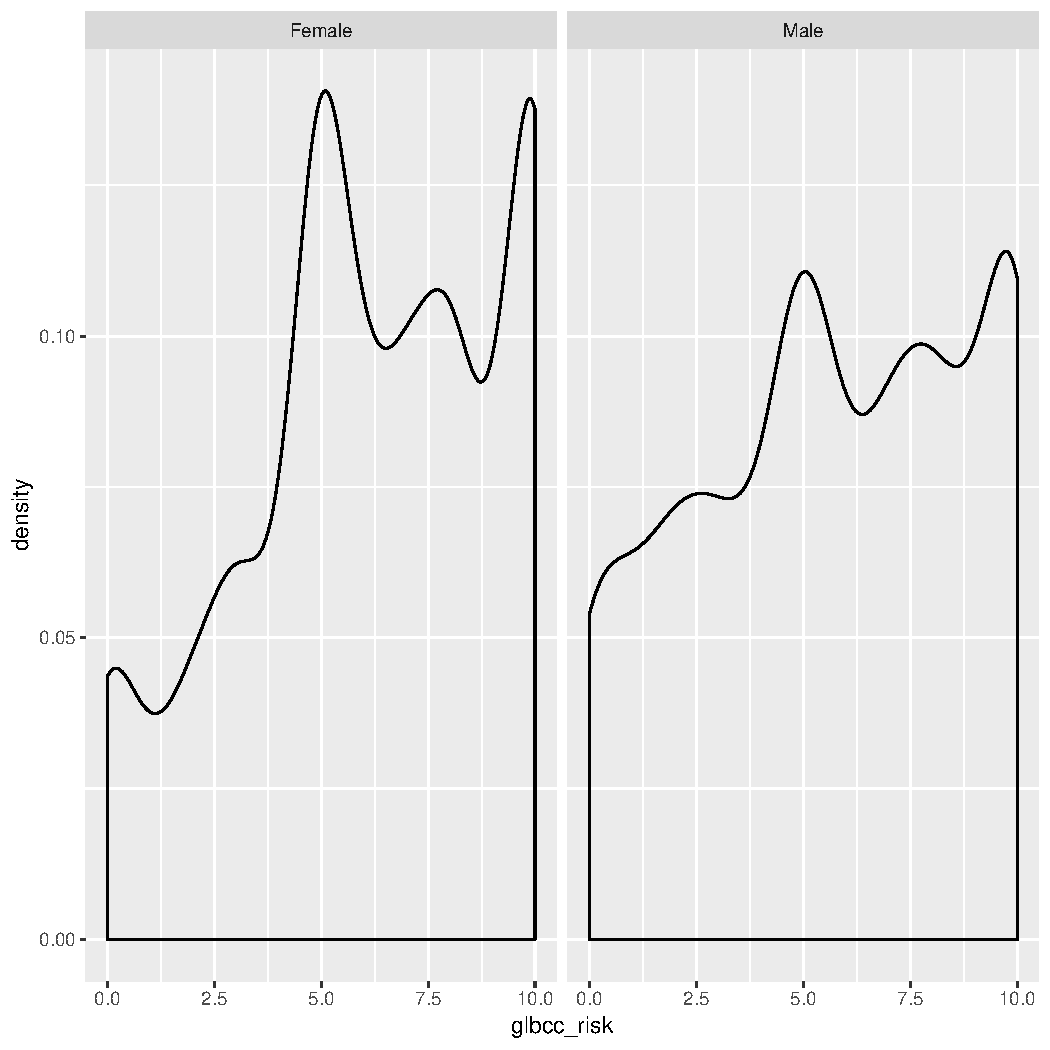
\includegraphics[width=4in, height=4in]{05_Inference/gendden.pdf}%filename
\caption{Density Plots of Climate Change Risk by Gender}
\end{figure}   

Based on the density plots, it appears that some differences exist between males and females regarding perceived climate change risk. We can also use the \texttt{by} command to see the \texttt{gccrsk} mean of climate change risk for males and females.
\begin{knitrout}
\definecolor{shadecolor}{rgb}{0.969, 0.969, 0.969}\color{fgcolor}\begin{kframe}
\begin{alltt}
\hlkwd{by}\hlstd{(ds}\hlopt{$}\hlstd{glbcc_risk, ds}\hlopt{$}\hlstd{f.gend, mean,} \hlkwc{na.rm} \hlstd{=} \hlnum{TRUE}\hlstd{)}
\end{alltt}
\begin{verbatim}
## ds$f.gend: Female
## [1] 6.134259
## -------------------------------------------------------- 
## ds$f.gend: Male
## [1] 5.670577
\end{verbatim}
\end{kframe}
\end{knitrout}
\begin{knitrout}
\definecolor{shadecolor}{rgb}{0.969, 0.969, 0.969}\color{fgcolor}\begin{kframe}
\begin{verbatim}
## [1] "Female" "Male"
\end{verbatim}
\end{kframe}
\end{knitrout}
Again there appears to be a difference, with females perceiving greater risk on average (6.13) than males (5.67). However we want to know whether these differences are \textbf{statistically significant}. To test for the statistical significance of the difference between groups, we use a $t$-test. 

\subsection{$t$-tests} 

The $t$-test is based in the $t$ distribution. The $t$ distribution, also known as the Student's $t$ distribution, is the probability 
distribution for \textit{sample} estimates. It has similar properties, and is related to, the normal distribution. The normal distribution is
based on a population where $\mu$ and $\sigma^2$ are known, however the $t$ distribution is based on a sample where $\mu$ and $\sigma^2$
are estimated, as the mean $\bar{X}$ and variance $s^2_x$. The mean of the $t$ distribution, like the normal distribution is $0$, but the
variance, $s^2_x$, is conditioned by $n-1$ \textbf{degrees of freedom}(df). Degrees of freedom are the values used to calculate a statistic that are "free" to vary.\footnote{In a difference of means test across two groups, we "use up" one observation when we separate the observations into two groups. Hence the denominator reflects the loss of that used up observation: n-1.} A $t$ distribution approaches the standard normal distribution as the number of degrees of freedom increase.

In brief, we want to know the difference of means between males and females, $d = \bar{X}_m-\bar{X}_f$ and if that difference is statistically
significant. This amounts to a hypothesis test where our working hypothesis, $H_1$, is that males are less likely than females to view climate
change as risky. The null hypothesis, $H_A$, is that there is no difference between males and females regarding the risks associated with climate
change. To test $H_1$ we use the $t$-test which is calculated: 
\begin{equation}
  \label{eq:t}
  t = \frac{\bar{X}_m-\bar{X}_f}{SE_d}
\end{equation}
\noindent Where $SE_d$ is the \textbf{standard error} of the estimated differences between the two groups.  To estimate $SE_d$ we need the SE of the estimated mean for each group. The SE is calculated: 
\begin{equation}
  \label{eq:se}
  SE = \frac{s}{\sqrt{n}}
\end{equation}
\noindent where $s$ is the s.d. of the variable. $H_1$ states that there is a difference between males and females, therefore under $H_1$ it is expected that $t > 0$ since zero is the mean of the $t$ distribution. However, under $H_A$ it is expected that $t = 0$. 

% t-test by hand
We can calculate this in \texttt{R}. First, we calculate the $n$ size for males and females. Then we calculate the SE for males and females. 
\begin{knitrout}
\definecolor{shadecolor}{rgb}{0.969, 0.969, 0.969}\color{fgcolor}\begin{kframe}
\begin{alltt}
\hlstd{n.total} \hlkwb{<-} \hlkwd{length}\hlstd{(ds}\hlopt{$}\hlstd{gender)}
\hlstd{nM} \hlkwb{<-} \hlkwd{sum}\hlstd{(ds}\hlopt{$}\hlstd{gender,} \hlkwc{na.rm} \hlstd{=} \hlnum{TRUE}\hlstd{)}
\hlstd{nF} \hlkwb{<-} \hlstd{n.total} \hlopt{-} \hlstd{nM}
\hlkwd{by}\hlstd{(ds}\hlopt{$}\hlstd{glbcc_risk, ds}\hlopt{$}\hlstd{f.gend, sd,} \hlkwc{na.rm} \hlstd{=} \hlnum{TRUE}\hlstd{)}
\end{alltt}
\begin{verbatim}
## ds$f.gend: Female
## [1] 2.981938
## -------------------------------------------------------- 
## ds$f.gend: Male
## [1] 3.180171
\end{verbatim}
\begin{alltt}
\hlstd{sdM} \hlkwb{<-} \hlnum{2.82}
\hlstd{seM} \hlkwb{<-} \hlnum{2.82}\hlopt{/}\hlstd{(}\hlkwd{sqrt}\hlstd{(nM))}
\hlstd{seM}
\end{alltt}
\begin{verbatim}
## [1] 0.08803907
\end{verbatim}
\begin{alltt}
\hlstd{sdF} \hlkwb{<-} \hlnum{2.35}
\hlstd{seF} \hlkwb{<-} \hlnum{2.35}\hlopt{/}\hlstd{(}\hlkwd{sqrt}\hlstd{(nF))}
\hlstd{seF}
\end{alltt}
\begin{verbatim}
## [1] 0.06025641
\end{verbatim}
\end{kframe}
\end{knitrout}

\noindent Next, we need to calculate the $SE_d$: 
\begin{equation}
  SE_d = \sqrt{SE^2_M+SE^2_F}  
\end{equation}
\begin{knitrout}
\definecolor{shadecolor}{rgb}{0.969, 0.969, 0.969}\color{fgcolor}\begin{kframe}
\begin{alltt}
\hlstd{seD} \hlkwb{<-} \hlkwd{sqrt}\hlstd{(seM}\hlopt{^}\hlnum{2} \hlopt{+} \hlstd{seF}\hlopt{^}\hlnum{2}\hlstd{)}
\hlstd{seD}
\end{alltt}
\begin{verbatim}
## [1] 0.1066851
\end{verbatim}
\end{kframe}
\end{knitrout}

\noindent Finally, we can calculate our $t$-score, and use the \texttt{t.test} function to check. 
\begin{knitrout}
\definecolor{shadecolor}{rgb}{0.969, 0.969, 0.969}\color{fgcolor}\begin{kframe}
\begin{alltt}
\hlkwd{by}\hlstd{(ds}\hlopt{$}\hlstd{glbcc_risk, ds}\hlopt{$}\hlstd{f.gend, mean,} \hlkwc{na.rm} \hlstd{=} \hlnum{TRUE}\hlstd{)}
\end{alltt}
\begin{verbatim}
## ds$f.gend: Female
## [1] 6.134259
## -------------------------------------------------------- 
## ds$f.gend: Male
## [1] 5.670577
\end{verbatim}
\begin{alltt}
\hlstd{meanF} \hlkwb{<-} \hlnum{6.96}
\hlstd{meanM} \hlkwb{<-} \hlnum{6.42}
\hlstd{t} \hlkwb{<-} \hlstd{(meanF} \hlopt{-} \hlstd{meanM)}\hlopt{/}\hlstd{seD}
\hlstd{t}
\end{alltt}
\begin{verbatim}
## [1] 5.061625
\end{verbatim}
\begin{alltt}
\hlkwd{t.test}\hlstd{(ds}\hlopt{$}\hlstd{glbcc_risk} \hlopt{~} \hlstd{ds}\hlopt{$}\hlstd{gender)}
\end{alltt}
\begin{verbatim}
## 
## 	Welch Two Sample t-test
## 
## data:  ds$glbcc_risk by ds$gender
## t = 3.6927, df = 2097.5, p-value = 0.0002275
## alternative hypothesis: true difference in means is not equal to 0
## 95 percent confidence interval:
##  0.2174340 0.7099311
## sample estimates:
## mean in group 0 mean in group 1 
##        6.134259        5.670577
\end{verbatim}
\end{kframe}
\end{knitrout}

The difference in the percieved risk between women and men, we have a $t$-value of 4.6. This result is greater than zero, as expected by $H_1$. In addition, as shown in the \texttt{t.test} output the \textbf{$p$-value}---the probability of obtaining our result if the population difference was $0$---is extremely low at .0002275} (that's the same as 2.275e-04). Therefore, we \textit{reject the null hypothesis} and concluded that there are differences (on average) in the ways that males and females perceive climate change risk.   

\section{Summary}
In this chapter we gained an understanding of inferential statistics, how to use them to place confidence intervals around an estimate, and got an overview of how to use them to test hypotheses. In the next chapter we turn, more formally, to testing hypotheses using crosstabs and by comparing means of different groups.  After that we continue to explore hypothesis testing and model building using regression analysis.






\chapter{Association of Variables}

The last chapter focused on the characterization of distributions of a single variable. We now turn to the associations between two or more variables. This chapter explores ways to measure and visualize associations between variables.   We start with ways to analyze the relations between nominal and ordinal level variables, using \textbf{cross-tabulation} in \textit{R}. Then, for interval level variables, we examine the use of the measures of the \textbf{covariance} and  \textbf{correlation} between pairs of variables. Next we examine hypothesis testing between two groups, where the focus in on how the groups differ, on average, with respect to an interval level variable. Finally, we discuss scatterplots as a way to visually explore differences between pairs of variables. 

\section{Cross-Tabulation}

To determine if there is an association between two variables measured at the nominal or ordinal levels we use cross-tabulation and a set of supporting statistics.  A cross-tabulation (or just crosstab) is a table that looks at the distribution of two variables simultaneously.   Table \ref{tab:IV_DV_Table} provides a sample layout of a 2 X 2 table.

\begin{table}[h]
\centering
\caption{Sample Table Layout} \label{tab:IV_DV_Table}
\begin{tabular}{|l|c|c|c|}
\hline
\diagbox[width=10em]{Dependent\\Variable}{Independent\\Variable} & IV - Low & IV - High & Total \\ \hline
DV - Low & 60\% & 40\% & 53\% \\ \hline
DV - High & 40\% & 60\% & 47\% \\ \hline
 & \begin{tabular}[c]{@{}l@{}}100\%\\ n = 200\end{tabular} & \begin{tabular}[c]{@{}l@{}}100\%\\ n=100\end{tabular} & n = 300 \\ \hline
\end{tabular}
\end{table}

As Table \ref{tab:IV_DV_Table} illustrates, a crosstab is set up so that the independent variable is on the top, forming columns, and the dependent variable is on the side, forming rows.   Toward the upper left hand corner of the table are the low, or negative variable categories.  Generally, a table will be displayed in percentage format.  The marginals for a table are the column totals and the row totals and are the same as a frequency distribution would be for that variable.   Each cross-classification reports how many observations have that shared characteristic.  The cross-classification groups are referred to as \textbf{cells}, so Table \ref{tab:IV_DV_Table} is a four-celled table.

A table like Table \ref{tab:IV_DV_Table} provides a basis to begin to answer the question of whether our independent and dependent variables are related.  Remember that our null hypothesis says there is no relationship between our IV and our DV.  Looking at Table \ref{tab:IV_DV_Table}, we can say of those low on the IV, 60\% of them will also be low on the DV; and that those high on the IV will be low on the DV 40\% of the time.  Our null hypothesis says there should be no difference, but in this case, there is a 20\% difference so it appears that our null hypothesis is incorrect.  What we learned in our inferential statistics chapter, though, tells us that it is still possible that the null hypothesis is true. The question is how likely is it that we could have a 20\% difference in our sample even if the null hypothesis is true?\footnote{To reiterate the general decision rule: if the probability that we could have a 20\% difference in our sample if the null hypothesis is true is less than .05 we will reject our null hypothesis.}

We use the \textbf{chi square statistic} to test our null hypothesis when using crosstabs.  To find chi square ($\chi^2$), we begin by assuming the null hypothesis to be true and find the expected frequencies for each cell in our table.   We do so using a posterior methodology based on the marginals for our dependent variable.   We see that 53\% of our total sample is low on the dependent variable.   If our null hypothesis is correct, then where one is on the independent variable should not matter so 53\% of those who are low on the IV should be low on the DV and 53\% of those who are high on the IV should be low on the DV.  Table \ref{tab:IV_DV_Table2} \& \ref{tab:IV_DV_Table3} illustrate this pattern.  To find the expected frequency for each cell, we simply multiply the expected cell percentage times the number of people in each category of the IV:  the expected frequency for the low-low cell is $.53 * 200 = 106$; for the low-high cell, it is $.47 * 200 = 94$; for the low-high cell it is $.53 * 100 = 53$; and for the high-high cell, the expected frequency is $.47 * 100 = 47$.  (See Table \ref{tab:IV_DV_Table2} \& \ref{tab:IV_DV_Table3})

The formula for the chi square takes the expected frequency for each of the cells and subtracts the observed frequency from it, squares those differences, divides by the expected frequency, and sums those values:

\begin{equation}
  \label{eq:chisquare}
\chi^2  = \sum \frac{(O-E)^2}{E}
  \end{equation}

\noindent where:\\
$\chi^2$  = The Test Statistic\\
$\sum$ = The Summation Operator \\ 
$O$ = Observed Frequencies \\
$E$ = Expected Frequencies \\

\begin{table}[h]
\centering
\caption{ Sample Null-Hypothesized Table Layout as Percentages} \label{tab:IV_DV_Table2}
\begin{tabular}{|l|c|c|c|}
\hline
\diagbox[width=10em]{Dependent\\Variable}{Independent\\Variable} & IV - Low & IV - High & Total \\ \hline
DV - Low & 53\% & 53\% & 53\% \\ \hline
DV - High & 47\% & 47\% & 47\% \\ \hline
 & \begin{tabular}[c]{@{}l@{}}100\%\\ n = 200\end{tabular} & \begin{tabular}[c]{@{}l@{}}100\%\\ n=100\end{tabular} & n = 300 \\ \hline
\end{tabular}
\end{table}

% second tables with values this may need to be combined with previous table.
\begin{table}[h]
\centering
\caption{ Sample Null-Hypothesized Table Layout as Counts} \label{tab:IV_DV_Table3}
\begin{tabular}{|l|c|c|c|}
\hline
\diagbox[width=10em]{Dependent\\Variable}{Independent\\Variable} & IV - Low & IV - High & Total \\ \hline
DV - Low & 106 & 53 & 159 \\ \hline
DV - High & 94 & 47 & 141 \\ \hline
 & 200 & 100 &  300 \\ \hline
\end{tabular}
\end{table}

Table \ref{tab:IV_DV_Table4} provides those calculations.   It shows a final chi square of 10.73.  With that chi square, we can go to a chi square table to determine whether to accept or reject the null hypothesis.  Before going to that chi square table, we need to figure out two things.  First, we need to determine the level of significance we want, presumably .05.  Second, we need to determine our degrees of freedom.  We will have more on that concept as we go on, but for now, know that it is your number of rows minus one times your number of columns minus one.  In this case we have $(2-1)(2-1) = 1$ degree of freedom.  
	 
\begin{table}[h]
\centering
\caption{Chi Square ($\chi^2$) Calculation } \label{tab:IV_DV_Table4}
\begin{tabular}{|l|c|c|c|c|}
\hline
Cell & Observed Freq & Expected Freq & $(O-E)^2$ & $\frac{(O-E)^2}{E}$ \\ \hline
low-low & 120 & 106 & 196 & 1.85 \\ \hline
low-high & 80 & 94 & 196 & 2.09 \\ \hline
high-low & 40 & 53 & 169 & 3.19 \\ \hline
high-high & 60 & 47 & 169 & 3.60 \\ \hline
Total &  &  &  & 10.73 \\ \hline
\end{tabular}
\end{table}

Table \ref{tab:chisquaretable} (at the end of this chapter) is a chi square table that shows the critical values for various levels of significance and degrees of freedom.   The critical value for one degree of freedom with a .05 level of significance is 3.84.  Since our chi square is larger than that we can reject our null hypothesis - there is less than a .05 probability that we could have found the results in our sample if there is no relationship in the population.  In fact, if we follow the row for one degree of freedom across, we see we can reject our null hypothesis even at the .005 level of significance and, almost but not quite, at the .001 level of significance.  

Having rejected the null hypothesis, we believe there is a relationship between the two variables, but we still want to know how strong that relationship is.   Measures of association are used to determine the strength of a relationship. One type of measure of association relies on a co-variation model as elaborated upon in Sections 6.2 and 6.3.  Co-variation models are directional models and require ordinal or interval level measures; otherwise, the variables have no direction.  Here we consider alternative models. 

If one or both of our variables is nominal we cannot specify directional change.  Still, we might see a recognizable pattern of change in one variable as the other variable varies.  Women might be more concerned about climate change than are men, for example. For that type of case, we may use a reduction in error or a \textbf{proportional reduction in error (PRE) model}.  We consider how much better we predict using a naive model (assuming no relationship) and compare it to how much better we predict when we use our independent variable to make that prediction.   These measures of association only range from $0 - 1.0$, since the sign otherwise indicates direction.  Generally, we use this type of measure when at least one our variables is nominal, but we will also use a PRE model measure, $r^2$, in regression analysis.  \textbf{Lambda} is a commonly used PRE-based measure of association for nominal level data, but it can underestimate the relationship in some circumstances. 

Another set of measures of association suitable for nominal level data is based on chi square.  \textbf{Cramer's V} is a simple chi square based indicator, but like chi square itself, its value is affected by the sample size and the dimensions of the table.  \textbf{Phi} corrects for sample size, but is appropriate only for a 2 X 2 table.  The \textbf{contingency coefficient}, C, also corrects for sample size and can be applied to larger tables, but requires a square table, i.e., the same number of rows and columns. 

If we have ordinal level data, we can use a co-variation model, but the specific model developed below in Section 6.3 looks at how observations are distributed around the means.  Since we cannot find a mean for ordinal level data, we need an alternative.  \textbf{Gamma} is commonly used with ordinal level data and provides a summary comparing how many observations fall around the diagonal in the table that supports a positive relationship (e.g. observations in the low-low cell and the high-high cells) as opposed to observations following the negative diagonal (e.g. the low-high cell and the high-low cells).  Gamma ranges from $-1.0$  to $+1.0$.\\

Crosstabulations and their associated statistics can be calculated using R.  In this example we use the Global Climate Change dataset (ds).  The dataset includes measures of survey respondents: gender (female = 0, male = 1); perceived risk posed by climate change or glbccrisk (0 = Not Risk; 10 = extreme risk), and political ideology (1 = strong liberal, 7 = strong conservative). Here we look at whether there is a relationship between gender and the glbccrisk variable.  The glbccrisk variable has eleven categories and to make the table more manageable we recode it to five categories.  

%  time permitting change the variable to age groups.

\begin{knitrout}
\definecolor{shadecolor}{rgb}{0.969, 0.969, 0.969}\color{fgcolor}\begin{kframe}
\begin{alltt}
\hlcom{# Factor the gender variable}
\hlstd{ds}\hlopt{$}\hlstd{f.gend} \hlkwb{<-} \hlkwd{factor}\hlstd{(ds}\hlopt{$}\hlstd{gender,} \hlkwc{levels} \hlstd{=} \hlkwd{c}\hlstd{(}\hlnum{0}\hlstd{,} \hlnum{1}\hlstd{),} \hlkwc{labels} \hlstd{=} \hlkwd{c}\hlstd{(}\hlstr{"Women"}\hlstd{,}
    \hlstr{"Men"}\hlstd{))}

\hlcom{# recode glbccrisk to five categories}
\hlkwd{library}\hlstd{(car)}
\hlstd{ds}\hlopt{$}\hlstd{r.glbcc_risk} \hlkwb{<-} \hlstd{car}\hlopt{::}\hlkwd{recode}\hlstd{(ds}\hlopt{$}\hlstd{glbcc_risk,} \hlstr{"0:1=1; 2:3=2; 4:6=3; 7:8:=4;
                          9:10=5; NA=NA"}\hlstd{)}
\end{alltt}
\end{kframe}
\end{knitrout}

Using the \texttt{table} function, we produce a frequency table reflecting the relationship between gender and the recoded glbccrisk variable.  

\begin{knitrout}
\definecolor{shadecolor}{rgb}{0.969, 0.969, 0.969}\color{fgcolor}\begin{kframe}
\begin{alltt}
\hlcom{# create the table}
\hlkwd{table}\hlstd{(ds}\hlopt{$}\hlstd{r.glbcc_risk, ds}\hlopt{$}\hlstd{f.gend)}
\end{alltt}
\begin{verbatim}
##    
##     Women Men
##   1   134 134
##   2   175 155
##   3   480 281
##   4   330 208
##   5   393 245
\end{verbatim}
\begin{alltt}
\hlcom{# create the table as an R Object}
\hlstd{glbcc.table} \hlkwb{<-} \hlkwd{table}\hlstd{(ds}\hlopt{$}\hlstd{r.glbcc_risk, ds}\hlopt{$}\hlstd{f.gend)}
\end{alltt}
\end{kframe}
\end{knitrout}

That table is difficult to interpret because of the different numbers of men and women.  To make that table more interpretable, we convert it to percentages using the \texttt{prop.table} function.   Looking at that table, we can see that there are more men at the lower end of the perceived risk scale and more women at the upper end.

\begin{knitrout}
\definecolor{shadecolor}{rgb}{0.969, 0.969, 0.969}\color{fgcolor}\begin{kframe}
\begin{alltt}
\hlcom{# Multiply by 100}
\hlkwd{prop.table}\hlstd{(glbcc.table,} \hlnum{2}\hlstd{)} \hlopt{*} \hlnum{100}
\end{alltt}
\begin{verbatim}
##    
##         Women       Men
##   1  8.862434 13.098729
##   2 11.574074 15.151515
##   3 31.746032 27.468231
##   4 21.825397 20.332356
##   5 25.992063 23.949169
\end{verbatim}
\end{kframe}
\end{knitrout}
  
The percentaged table suggests that there is a relationship between the two variables, but also illustrates the challenge of relying on percentage differences to determine the significance of that relationship.  So, to test our null hypothesis we calculate our chi square using the chisq.test function.  

\begin{knitrout}
\definecolor{shadecolor}{rgb}{0.969, 0.969, 0.969}\color{fgcolor}\begin{kframe}
\begin{alltt}
\hlcom{# Chi Square Test}
\hlkwd{chisq.test}\hlstd{(glbcc.table)}
\end{alltt}
\begin{verbatim}
## 
## 	Pearson's Chi-squared test
## 
## data:  glbcc.table
## X-squared = 21.729, df = 4, p-value = 0.0002269
\end{verbatim}
\end{kframe}
\end{knitrout}

R reports our chi square to equal 21.73.  It also tells us that we have 4 degrees of freedom and a p value of .0002269.  Since that p value is substantially less than .05, we can reject our null hypothesis with great confidence.  There is, evidently, a relationship between gender and percieved risk of climate change.

Finally, we want to know how strong the relationship is.  We use the \texttt{assocstats} function to get several measures of association.   Since the table is not a 2 X 2 table nor square, neither phi not the contingency coefficient is appropriate, but we can report Cramer's V.  Cramer's V is .093, indicating a relatively weak relationship between gender and the perceived global climate change risk variable.

\begin{knitrout}
\definecolor{shadecolor}{rgb}{0.969, 0.969, 0.969}\color{fgcolor}\begin{kframe}
\begin{alltt}
\hlkwd{library}\hlstd{(vcd)}
\hlkwd{assocstats}\hlstd{(glbcc.table)}
\end{alltt}
\begin{verbatim}
##                     X^2 df   P(> X^2)
## Likelihood Ratio 21.494  4 0.00025270
## Pearson          21.729  4 0.00022695
## 
## Phi-Coefficient   : NA 
## Contingency Coeff.: 0.092 
## Cramer's V        : 0.093
\end{verbatim}
\end{kframe}
\end{knitrout}

\subsection{Crosstabulation and Control}

In Chapter 2 we talked about the importance of experimental control if we want to make causal statements.  In experimental designs we rely on physical control and randomization to provide that control which give us confidence in the causal nature of any relationship we find.  With quasi-experimental designs, however, we do not have that type of control and have to wonder whether a relationship that we find might be spurious.   At that point, we promised that the situation is not hopeless with quasi-experimental designs and that there are statistical substitutes for the control naturally afforded us in experimental designs.  In this section, we will describe that process when using crosstabulation.  We will first look at some hypothetical data to get some clean examples of what might happen when you control for an alternative explanatory variable before looking at a real example using R.

The process used to control for an alternative explanatory variable, commonly referred to as a third variable, is straightforward.   To control for a third variable, we first construct our original table between our independent and dependent variables.  Then we sort our data into subsets based on the categories of our third variable and reconstruct new tables using our IV and DV for each subset of our data. 

Suppose we hypothesize that people who are contacted about voting are more likely to vote.  Table \ref{tab:TableWithControl1} illustrates what we might find.  (Remember all of these data are fabricated to illustrate our points.)  According to the first table, people who are contacted are 50\% more likely to vote than those who are not.  But, a skeptic might say campaigns target previous voters for contact and that previous voters are more likely to vote in subsequent elections.  That skeptic is making the argument that the relationship between contact and voting is spurious and that the true cause of voting is voting history.  To test that theory, we control for voting history by sorting respondents into two sets -- those who voted in the last election and those who did not.  We then reconstruct the original table for the two sets of respondents.   The new tables indicate that previous voters are 50\% more likely to vote when contacted, and that those who did not vote previously are 50\% more likely to vote when contacted.   The skeptic is wrong; the pattern found in our original data persists even after controlling.  We still remain reluctant to use causal language because another skeptic might have another alternative explanation (which would require us to go through the same process with the new third variable), but we do have more confidence in the possible causal nature of the relationship between contact and voting.

The next example tests the hypothesis that those who are optimistic about the future are more likely to vote for the incumbent than those who are pessimistic.  Table \ref{tab:TableWithControl2} shows that optimistic people are 25\% more likely to vote for the incumbent than are pessimistic people.   But our skeptic friend might argue that feelings about the world are not nearly as important as real life conditions.  People with jobs vote for the incumbent more often than those without a job and, of course, those with a job are more likely to feel good about the world.  To test that alternative, we control for whether the respondent has a job and reconstruct new tables.  When we do, we find that among those with a job, 70\% vote for the incumbent - regardless of their level of optimism about the world.  And, among those without a job, 40\% vote for the incumbent, regardless of their optimism.  In other words, after controlling for job status, there is no relationship between level of optimism and voting behavior.  The original relationship was spurious.

\begin{table}[h]
\centering
\caption{Controlling for a Third Variable: Nothing Changes} \label{tab:TableWithControl1}
\begin{tabular}{lcc}
All Respondents &  &  \\ \hline
\multicolumn{1}{|l|}{} & \multicolumn{1}{c|}{Not Contacted} & \multicolumn{1}{c|}{Contacted} \\ \hline
\multicolumn{1}{|l|}{Not Vote} & \multicolumn{1}{c|}{75\%} & \multicolumn{1}{c|}{25\%} \\ \hline
\multicolumn{1}{|l|}{Vote} & \multicolumn{1}{c|}{25\%} & \multicolumn{1}{c|}{75\%} \\ \hline
\multicolumn{1}{|l|}{} & \multicolumn{1}{c|}{100\%} & \multicolumn{1}{c|}{100\%} \\ \hline
&  &  \\ 
Respondents who Voted in the Last Election &  &  \\ \hline
\multicolumn{1}{|l|}{} & \multicolumn{1}{c|}{Not Contacted} & \multicolumn{1}{c|}{Contacted} \\ \hline
\multicolumn{1}{|l|}{Not Vote} & \multicolumn{1}{c|}{75\%} & \multicolumn{1}{c|}{25\%} \\ \hline
\multicolumn{1}{|l|}{Vote} & \multicolumn{1}{c|}{25\%} & \multicolumn{1}{c|}{75\%} \\ \hline
\multicolumn{1}{|l|}{} & \multicolumn{1}{c|}{100\%} & \multicolumn{1}{c|}{100\%} \\ \hline
% \multicolumn{1}{|l|}{} & \multicolumn{1}{c|}{} & \multicolumn{1}{c|}{} \\ \hline
 &  &  \\
Respondents who Did Not Vote in the Last Election &  &  \\ \hline
\multicolumn{1}{|l|}{} & \multicolumn{1}{c|}{Not Contacted} & \multicolumn{1}{c|}{Contacted} \\ \hline
\multicolumn{1}{|l|}{Not Vote} & \multicolumn{1}{c|}{75\%} & \multicolumn{1}{c|}{25\%} \\ \hline
\multicolumn{1}{|l|}{Vote} & \multicolumn{1}{c|}{25\%} & \multicolumn{1}{c|}{75\%} \\ \hline
\multicolumn{1}{|l|}{} & \multicolumn{1}{c|}{100\%} & \multicolumn{1}{c|}{100\%} \\ \hline
\end{tabular}
\end{table}

\begin{table}[h]
\centering
\caption{Controlling for a Third Variable: Spurious} \label{tab:TableWithControl2}
\begin{tabular}{lcc}
\hline
\multicolumn{1}{|l|}{All Respondent} & \multicolumn{1}{c|}{} & \multicolumn{1}{c|}{} \\ \hline
\multicolumn{1}{|l|}{} & \multicolumn{1}{c|}{Pessimistic} & \multicolumn{1}{c|}{Optimistic} \\ \hline
\multicolumn{1}{|l|}{Not Vote Incumbent} & \multicolumn{1}{c|}{55\%} & \multicolumn{1}{c|}{30\%} \\ \hline
\multicolumn{1}{|l|}{Vote Incumbent} & \multicolumn{1}{c|}{45\%} & \multicolumn{1}{c|}{70\%} \\ \hline
\multicolumn{1}{|l|}{} & \multicolumn{1}{c|}{100\%} & \multicolumn{1}{c|}{100\%} \\ \hline
 &  &  \\ \hline
\multicolumn{1}{|l|}{Have a Job} & \multicolumn{1}{c|}{} & \multicolumn{1}{c|}{} \\ \hline
\multicolumn{1}{|l|}{} & \multicolumn{1}{c|}{Pessimistic} & \multicolumn{1}{c|}{Optimistic} \\ \hline
\multicolumn{1}{|l|}{Not Vote Incumbent} & \multicolumn{1}{c|}{30\%} & \multicolumn{1}{c|}{30\%} \\ \hline
\multicolumn{1}{|l|}{Vote Incumbent} & \multicolumn{1}{c|}{70\%} & \multicolumn{1}{c|}{70\%} \\ \hline
\multicolumn{1}{|l|}{} & \multicolumn{1}{c|}{100\%} & \multicolumn{1}{c|}{100\%} \\ \hline
 &  &  \\ \hline
\multicolumn{1}{|l|}{Not Have a Job} & \multicolumn{1}{c|}{} & \multicolumn{1}{c|}{} \\ \hline
\multicolumn{1}{|l|}{} & \multicolumn{1}{c|}{Pessimistic} & \multicolumn{1}{c|}{Optimistic} \\ \hline
\multicolumn{1}{|l|}{Not Vote Incumbent} & \multicolumn{1}{c|}{60\%} & \multicolumn{1}{c|}{60\%} \\ \hline
\multicolumn{1}{|l|}{Vote Incumbent} & \multicolumn{1}{c|}{40\%} & \multicolumn{1}{c|}{40\%} \\ \hline
\multicolumn{1}{|l|}{} & \multicolumn{1}{c|}{100\%} & \multicolumn{1}{c|}{100\%} \\ \hline
\end{tabular}
\end{table}

A third outcome of controlling for a third variable might be some form of interaction or specification effect.  The third variable affects how the first two are related, but it does not completely undermine the original relationship.  For example, we might find the original relationship to be stronger for one category of the control variable than another - or even to be present in one case and not the other.   Or, the pattern might suggest that both variables have an influence on the dependent variable, looking like some form of joint causation.  In fact, it is possible for your relationship to appear to be null in your original table, but when you control you might find a positive relationship for one category of your control variable and negative for another.   

Using an example from the Climate and Weather survey, we might hypothesize that liberals are more likely to think that greenhouse gases are causing global warming.   We start by recoding ideology from 7 levels to 3, then constructing first a frequency table, then a percentage table of the relationship.
  
\begin{knitrout}
\definecolor{shadecolor}{rgb}{0.969, 0.969, 0.969}\color{fgcolor}\begin{kframe}
\begin{alltt}
\hlcom{# recode variables ideology to 3 categories}
\hlkwd{library}\hlstd{(car)}
\hlstd{ds}\hlopt{$}\hlstd{r.ideol} \hlkwb{<-} \hlstd{car}\hlopt{::}\hlkwd{recode}\hlstd{(ds}\hlopt{$}\hlstd{ideol,} \hlstr{"1:2=1; 3:5=2; 6:7=3; NA=NA"}\hlstd{)}

\hlcom{# factor the variables to add labels.}
\hlstd{ds}\hlopt{$}\hlstd{f.ideol} \hlkwb{<-} \hlkwd{factor}\hlstd{(ds}\hlopt{$}\hlstd{r.ideol,} \hlkwc{levels} \hlstd{=} \hlkwd{c}\hlstd{(}\hlnum{1}\hlstd{,} \hlnum{2}\hlstd{,} \hlnum{3}\hlstd{),} \hlkwc{labels} \hlstd{=} \hlkwd{c}\hlstd{(}\hlstr{"Liberal"}\hlstd{,}
    \hlstr{"Moderate"}\hlstd{,} \hlstr{"Conservative"}\hlstd{))}
\hlstd{ds}\hlopt{$}\hlstd{f.glbcc} \hlkwb{<-} \hlkwd{factor}\hlstd{(ds}\hlopt{$}\hlstd{glbcc,} \hlkwc{levels} \hlstd{=} \hlkwd{c}\hlstd{(}\hlnum{0}\hlstd{,} \hlnum{1}\hlstd{),} \hlkwc{labels} \hlstd{=} \hlkwd{c}\hlstd{(}\hlstr{"GLBCC No"}\hlstd{,}
    \hlstr{"GLBCC Yes"}\hlstd{))}

\hlcom{# 3 Two variable table glbcc~ideology}
\hlstd{v2.glbcc.table} \hlkwb{<-} \hlkwd{table}\hlstd{(ds}\hlopt{$}\hlstd{f.glbcc, ds}\hlopt{$}\hlstd{f.ideol)}
\hlstd{v2.glbcc.table}
\end{alltt}
\begin{verbatim}
##            
##             Liberal Moderate Conservative
##   GLBCC No       26      322          734
##   GLBCC Yes     375      762          305
\end{verbatim}
\end{kframe}
\end{knitrout}

\begin{knitrout}
\definecolor{shadecolor}{rgb}{0.969, 0.969, 0.969}\color{fgcolor}\begin{kframe}
\begin{alltt}
\hlcom{# Percentages by Column}
\hlkwd{prop.table}\hlstd{(v2.glbcc.table,} \hlnum{2}\hlstd{)} \hlopt{*} \hlnum{100}
\end{alltt}
\begin{verbatim}
##            
##               Liberal  Moderate Conservative
##   GLBCC No   6.483791 29.704797    70.644851
##   GLBCC Yes 93.516209 70.295203    29.355149
\end{verbatim}
\end{kframe}
\end{knitrout}

\noindent It appears that our hypothesis is supported as there is more than a 40\% difference between liberals and conservatives with moderates in between, but let's consider the chi square before reject our null hypothesis:
\begin{knitrout}
\definecolor{shadecolor}{rgb}{0.969, 0.969, 0.969}\color{fgcolor}\begin{kframe}
\begin{alltt}
\hlcom{# Chi-squared}
\hlkwd{chisq.test}\hlstd{(v2.glbcc.table,} \hlkwc{correct} \hlstd{=} \hlnum{FALSE}\hlstd{)}
\end{alltt}
\begin{verbatim}
## 
## 	Pearson's Chi-squared test
## 
## data:  v2.glbcc.table
## X-squared = 620.76, df = 2, p-value < 0.00000000000000022
\end{verbatim}
\end{kframe}
\end{knitrout}

\noindent The chi square is very large and our p-value, very small. We can reject our null hypothesis with great confidence.  Next, we consider the strength of association, using Cramer's V (since either Phi nor the contingency coefficient is appropriate for a 3 X 2 table):

\begin{knitrout}
\definecolor{shadecolor}{rgb}{0.969, 0.969, 0.969}\color{fgcolor}\begin{kframe}
\begin{alltt}
\hlcom{# Cramer's V}
\hlkwd{library}\hlstd{(vcd)}
\hlkwd{assocstats}\hlstd{(v2.glbcc.table)}
\end{alltt}
\begin{verbatim}
##                     X^2 df P(> X^2)
## Likelihood Ratio 678.24  2        0
## Pearson          620.76  2        0
## 
## Phi-Coefficient   : NA 
## Contingency Coeff.: 0.444 
## Cramer's V        : 0.496
\end{verbatim}
\end{kframe}
\end{knitrout}

\noindent The Cramer's V value of .496 indicates that we have a strong relationship between political ideology and beliefs about climate change.\\

We might, though, want to look at gender as a control variable since we know gender is related both to perceptions on the climate and ideology.  First we need to generate a new table with the control variable gender added.  We start by factoring the gender variable.

\begin{knitrout}
\definecolor{shadecolor}{rgb}{0.969, 0.969, 0.969}\color{fgcolor}\begin{kframe}
\begin{alltt}
\hlcom{# factor the variables to add labels.}
\hlstd{ds}\hlopt{$}\hlstd{f.gend} \hlkwb{<-} \hlkwd{factor}\hlstd{(ds}\hlopt{$}\hlstd{gend,} \hlkwc{levels} \hlstd{=} \hlkwd{c}\hlstd{(}\hlnum{0}\hlstd{,} \hlnum{1}\hlstd{),} \hlkwc{labels} \hlstd{=} \hlkwd{c}\hlstd{(}\hlstr{"Women"}\hlstd{,}
    \hlstr{"Men"}\hlstd{))}
\end{alltt}
\end{kframe}
\end{knitrout}

\noindent Then we create the new table.  The R output is shown, in which the line ``\#\# ,  ,  = Women" indicates the results for women and ``\#\# ,  ,  = Men" displays the results for men.

\begin{knitrout}
\definecolor{shadecolor}{rgb}{0.969, 0.969, 0.969}\color{fgcolor}\begin{kframe}
\begin{alltt}
\hlcom{# 3 Two variable table glbcc~ideology+gend}
\hlstd{v3.glbcc.table} \hlkwb{<-} \hlkwd{table}\hlstd{(ds}\hlopt{$}\hlstd{f.glbcc, ds}\hlopt{$}\hlstd{f.ideol, ds}\hlopt{$}\hlstd{f.gend)}
\hlstd{v3.glbcc.table}
\end{alltt}
\begin{verbatim}
## , ,  = Women
## 
##            
##             Liberal Moderate Conservative
##   GLBCC No       18      206          375
##   GLBCC Yes     239      470          196
## 
## , ,  = Men
## 
##            
##             Liberal Moderate Conservative
##   GLBCC No        8      116          358
##   GLBCC Yes     136      292          109
\end{verbatim}
\end{kframe}
\end{knitrout}


\begin{knitrout}
\definecolor{shadecolor}{rgb}{0.969, 0.969, 0.969}\color{fgcolor}\begin{kframe}
\begin{alltt}
\hlcom{# Percentages by Column for Women}
\hlkwd{prop.table}\hlstd{(v3.glbcc.table[, ,} \hlnum{1}\hlstd{],} \hlnum{2}\hlstd{)} \hlopt{*} \hlnum{100}
\end{alltt}
\begin{verbatim}
##            
##               Liberal  Moderate Conservative
##   GLBCC No   7.003891 30.473373    65.674256
##   GLBCC Yes 92.996109 69.526627    34.325744
\end{verbatim}
\begin{alltt}
\hlkwd{chisq.test}\hlstd{(v3.glbcc.table[, ,} \hlnum{1}\hlstd{])}
\end{alltt}
\begin{verbatim}
## 
## 	Pearson's Chi-squared test
## 
## data:  v3.glbcc.table[, , 1]
## X-squared = 299.39, df = 2, p-value < 0.00000000000000022
\end{verbatim}
\begin{alltt}
\hlkwd{assocstats}\hlstd{(v3.glbcc.table[, ,} \hlnum{1}\hlstd{])}
\end{alltt}
\begin{verbatim}
##                     X^2 df P(> X^2)
## Likelihood Ratio 326.13  2        0
## Pearson          299.39  2        0
## 
## Phi-Coefficient   : NA 
## Contingency Coeff.: 0.407 
## Cramer's V        : 0.446
\end{verbatim}
\end{kframe}
\end{knitrout}

\begin{knitrout}
\definecolor{shadecolor}{rgb}{0.969, 0.969, 0.969}\color{fgcolor}\begin{kframe}
\begin{alltt}
\hlcom{# Percentages by Column for Men}
\hlkwd{prop.table}\hlstd{(v3.glbcc.table[, ,} \hlnum{2}\hlstd{],} \hlnum{2}\hlstd{)} \hlopt{*} \hlnum{100}
\end{alltt}
\begin{verbatim}
##            
##               Liberal  Moderate Conservative
##   GLBCC No   5.555556 28.431373    76.659529
##   GLBCC Yes 94.444444 71.568627    23.340471
\end{verbatim}
\begin{alltt}
\hlkwd{chisq.test}\hlstd{(v3.glbcc.table[, ,} \hlnum{2}\hlstd{])}
\end{alltt}
\begin{verbatim}
## 
## 	Pearson's Chi-squared test
## 
## data:  v3.glbcc.table[, , 2]
## X-squared = 320.43, df = 2, p-value < 0.00000000000000022
\end{verbatim}
\begin{alltt}
\hlkwd{assocstats}\hlstd{(v3.glbcc.table[, ,} \hlnum{2}\hlstd{])}
\end{alltt}
\begin{verbatim}
##                     X^2 df P(> X^2)
## Likelihood Ratio 353.24  2        0
## Pearson          320.43  2        0
## 
## Phi-Coefficient   : NA 
## Contingency Coeff.: 0.489 
## Cramer's V        : 0.561
\end{verbatim}
\end{kframe}
\end{knitrout}
%see note               

For both men and women, we still see more than a 40\% difference and the p value for both tables chi square is 2.2e-16 and both Cramer's V's are greater than .30.  It is clear that even when controlling for gender, there is a robust relationship between ideology and glbcc.  But, those tables also suggest that women are slightly more inclined to see greenhouse gases playing a role in climate change than are men.   We may have an instance of joint causation -- where both ideology and gender affect (``cause" is still too strong a word) views on the impact of greenhouse gases on climate change.

Crosstabs, chi square, and measures of association are used with nominal and ordinal data to get an overview of a relationship, its statistical significance, and the strength of a relationship.  In the next section we turn to ways to consider the same set of questions with interval level data, before turning to the more advanced technique of regression analysis in Part 2 of this book.  

\section{Covariance}

Covariance is a simple measure of the way two variables move together, or ``co-vary".  The covariance of two variables, $X$ and $Y$, can be expressed in population notation as: 
\begin{equation}
cov(X,Y) = E[(X-\mu_{x})(Y-\mu_{y})]  
\end{equation}
Therefore, the covariance between $X$ and $Y$ is simply the product of
the variation of $X$ around its expected value,
and the variation of $Y$
around its expected value.
The sample covariance is expressed as: 
\begin{equation}
cov(X,Y) = \frac{\sum (X-\bar{X})(Y-\bar{Y})}{(n-1)}   
\end{equation}
   
Covariance can be positive, negative, and zero. If the covariance is positive \textit{both variables move in the same direction},
therefore if $X$ increases $Y$ increases or if $X$ decreases $Y$ decreases. Negative covariance means that the \textit{variables move
  in the opposite direction}; if $X$ increases $Y$ decreases. Finally, zero covariance indicates that there is no covariance between $X$ and
$Y$.

\section{Correlation} 

Correlation is closely related to covariance. In essence, correlation standardizes covariance so it can be compared across variables. Correlation is represented by a correlation coefficient $\rho$, and is calculated by dividing the covariance of the two variables by the product of their standard deviations. For populations it is expressed as:

\begin{equation}
\rho = \frac{cov(X,Y)}{\sigma_{x} \sigma_{y}}  
\end{equation}
For samples it is expressed as: 
\begin{equation}
r = \frac{\sum (X-\bar{X})(Y-\bar{Y})/(n-1)}{s_{x}s_{y}}  
\end{equation}

Like covariance, correlations can be positive, negative, and zero. The possible values of the correlation coefficient $r$, range
from -1, perfect negative relationship to 1, perfect positive relationship. If $r=0$, that indicates no correlation.  Correlations can be calculated in \texttt{R}, using the \texttt{cor} function. 

\begin{knitrout}
\definecolor{shadecolor}{rgb}{0.969, 0.969, 0.969}\color{fgcolor}\begin{kframe}
\begin{alltt}
\hlstd{ds} \hlopt \hlkwd{select}\hlstd{(age, education, ideol, glbcc_risk)} \hlopt \hlkwd{na.omit}\hlstd{()} \hlopt
    \hlkwd{cor}\hlstd{()}
\end{alltt}
\begin{verbatim}
##                    age   education       ideol  glbcc_risk
## age         1.00000000 -0.06149090  0.08991177 -0.07514098
## education  -0.06149090  1.00000000 -0.13246843  0.09115774
## ideol       0.08991177 -0.13246843  1.00000000 -0.59009431
## glbcc_risk -0.07514098  0.09115774 -0.59009431  1.00000000
\end{verbatim}
\end{kframe}
\end{knitrout}

Note that each variable is perfectly (and positively) correlated with itself - naturally! Age is slightly and surprisingly negatively correlated with education (-0.06) and unsurprisingly positively political ideology (+0.09). What this means is that, in this dataset and on average, older people are slightly less educated and more conservative than younger people. Now notice the correlation coefficient for the relationship between ideology and perceived risk of climate change (glbccrisk). This correlation (-0.59) indicates that on average, the more conservative the individual is, the less risky climate change is perceived to be.

%% chi-square dicussion 

%% anova ?? 

\section{Scatterplots}

As noted earlier, it is often useful to try and see patterns between two variables. We examined the density plots of males and females with regard to climate change risk, then we tested these differences for statistical significance. However, we often want to know more than the mean difference between groups; we often want to know if differences exist for variables with several possible values. For example, here we examine the relationship between ideology and glbcc risk. One of the more efficient ways to do this is to produce a scatterplot. %Use geom_jitter. This is because ideology and glbcc risk are discrete variables(i.e., whole numbers), so we need to ``jitter" the data. If your values are continuous, use \texttt{geom_point}.\footnote{That means a ``jit" (a very small value) is applied to each observed point on the plot, so
%ou can see observations that are ``stacked" on the same coordinate. Ha! Just kidding; they're not called jits. We don't know what they're called. But they ought to be called jits.} The result is shown in Figure \ref{fig:scatjit}.  

\begin{knitrout}
\definecolor{shadecolor}{rgb}{0.969, 0.969, 0.969}\color{fgcolor}\begin{kframe}
\begin{alltt}
\hlstd{ds} \hlopt \hlkwd{ggplot}\hlstd{(}\hlkwd{aes}\hlstd{(ideol, glbcc_risk))} \hlopt{+} \hlkwd{geom_jitter}\hlstd{(}\hlkwc{shape} \hlstd{=} \hlnum{1}\hlstd{)}
\end{alltt}
\end{kframe}
\end{knitrout}

\begin{figure}[!htp]
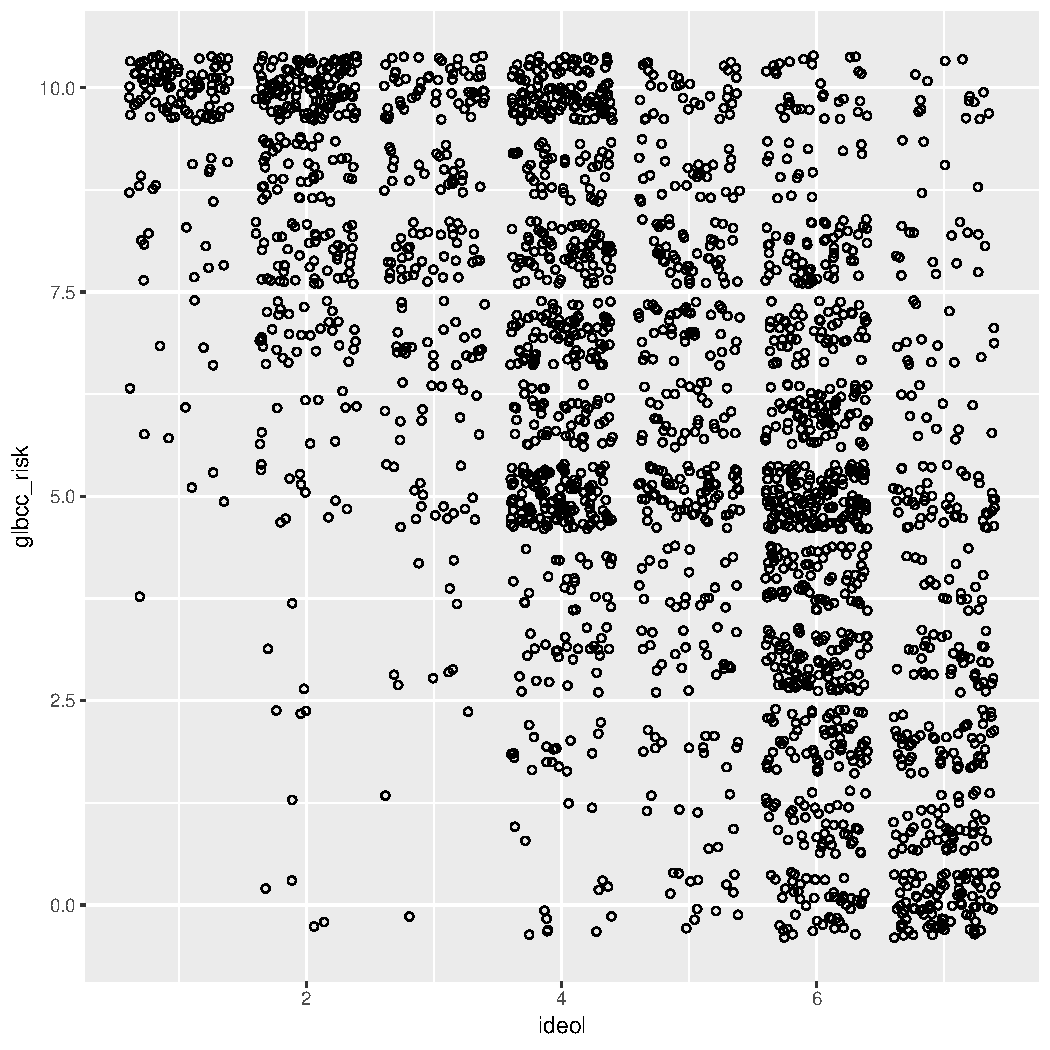
\includegraphics[width=3.5in, height=3.5in]{06_Association/scatjit.pdf}%filename
\caption{Scatterplot of Ideology and glbcc Risk \label{fig:scatjit}}
\end{figure}   

We can see that the density of values indicate that strong liberals---$1$'s on the ideology scale---tend to view climate change as quite risky, whereas strong conservatives---$7$'s on the ideology scale---tend to view climate change as less risky. Like our previous example, we want to know more about the nature of this relationship. Therefore, we can plot a regression line and a ``loess" line. These lines are the linear and nonlinear estimates of the relationship between political ideology and perceived risk of climate change. We'll have more to say about the linear estimates when we turn to regression analysis in the next chapter. %We can add to the previous visualization by including \texttt{geom_smooth} and indicating a "loess" line or an "lm" line. 

% note there is discussion of missing data in the Applied Regression book by Fox - Page 65-67.

\begin{knitrout}
\definecolor{shadecolor}{rgb}{0.969, 0.969, 0.969}\color{fgcolor}\begin{kframe}
\begin{alltt}
\hlstd{ds} \hlopt \hlkwd{drop_na}\hlstd{(glbcc_risk, ideol)} \hlopt \hlkwd{ggplot}\hlstd{(}\hlkwd{aes}\hlstd{(ideol, glbcc_risk))} \hlopt{+}
    \hlkwd{geom_jitter}\hlstd{(}\hlkwc{shape} \hlstd{=} \hlnum{1}\hlstd{)} \hlopt{+} \hlkwd{geom_smooth}\hlstd{(}\hlkwc{method} \hlstd{=} \hlstr{"loess"}\hlstd{,} \hlkwc{color} \hlstd{=} \hlstr{"green"}\hlstd{)} \hlopt{+}
    \hlkwd{geom_smooth}\hlstd{(}\hlkwc{method} \hlstd{=} \hlstr{"lm"}\hlstd{,} \hlkwc{color} \hlstd{=} \hlstr{"red"}\hlstd{)}
\hlkwd{dev.off}\hlstd{()}
\end{alltt}
\end{kframe}
\end{knitrout}

\begin{figure}[!htp]
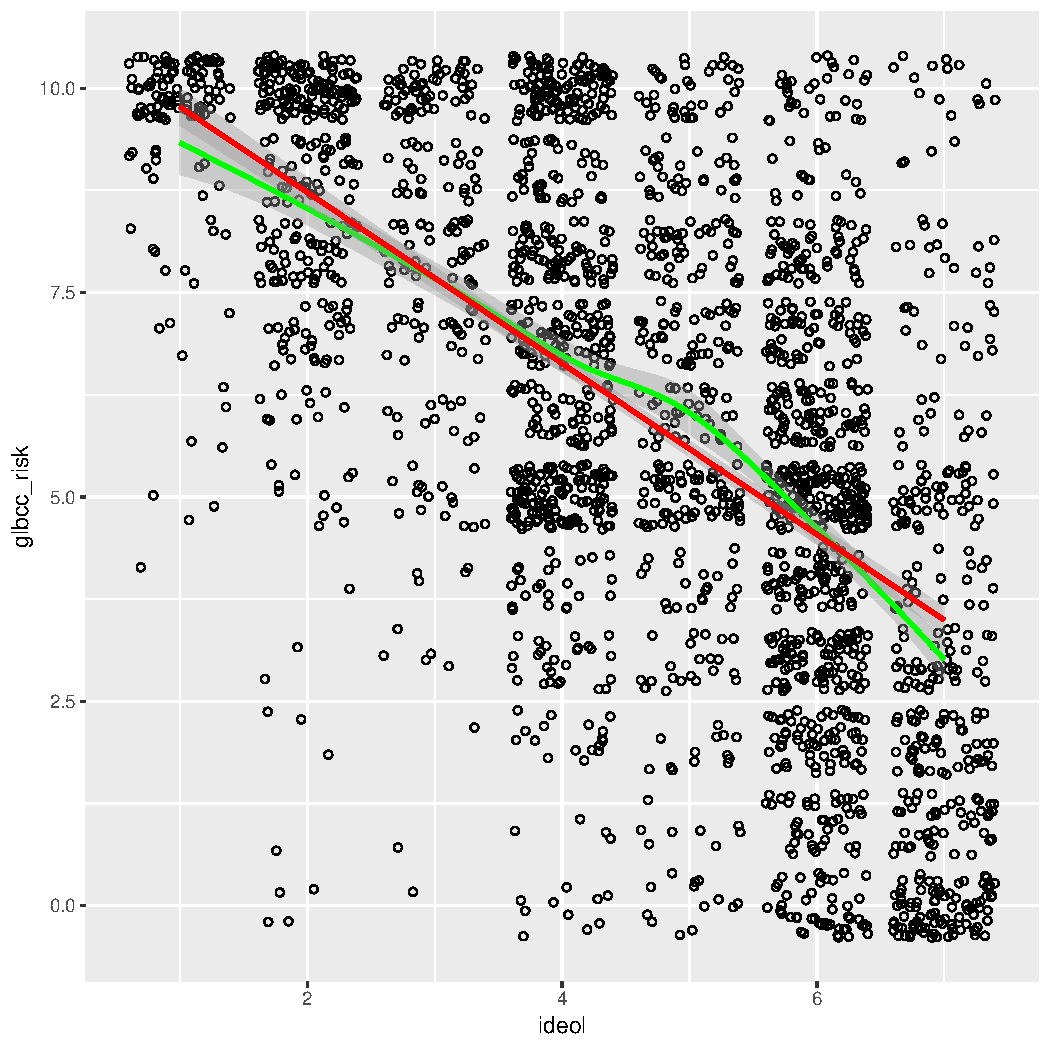
\includegraphics[width=3.5in, height=3.5in]{06_Association/scatjit2.pdf}%filename
\caption{Scatterplot of Ideology and GLBCC Risk with Regression Line and Lowess Line}
\end{figure}   

Note that the regression lines both slope downward, with average perceived risk  ranging from over 8 for the strong liberals (ideology=1) to less than 5 for strong conservatives (ideology=7). This illustrates how scatterplots can provide information about the nature of the relationship between two variables. We will take the next step -- to bivariate regression analysis -- in the next chapter.

\newpage
% Please add the following required packages to your document preamble:
% \usepackage{graphicx}
\begin{table}[h]
\caption{Appendix 6.1: Chi Square Table}
\label{tab:chisquaretable}
\resizebox{\textwidth}{!}{%
\begin{tabular}{|l|c|c|c|c|c|c|c|c|c|c|c|c|}
\hline
df & \multicolumn{12}{c|}{P-Value} \\ \hline
df & 0.25 & 0.20 & 0.15 & 0.10 & 0.05 & 0.025 & 0.02 & 0.01 & 0.005 & 0.0025 & 0.001 & 0.0005 \\ \hline
1 & 1.32 & 1.64 & 2.07 & 2.71 & 3.84 & 5.02 & 5.41 & 6.63 & 7.88 & 9.14 & 10.83 & 12.12 \\ \hline
2 & 2.77 & 3.22 & 3.79 & 4.61 & 5.99 & 7.38 & 7.82 & 9.21 & 10.60 & 11.98 & 13.82 & 15.20 \\ \hline
3 & 4.11 & 4.64 & 5.32 & 6.25 & 7.81 & 9.35 & 9.84 & 11.34 & 12.84 & 14.32 & 16.27 & 17.73 \\ \hline
4 & 5.39 & 5.59 & 6.74 & 7.78 & 9.49 & 11.14 & 11.67 & 13.23 & 14.86 & 16.42 & 18.47 & 20.00 \\ \hline
5 & 6.63 & 7.29 & 8.12 & 9.24 & 11.07 & 12.83 & 13.33 & 15.09 & 16.75 & 18.39 & 20.51 & 22.11 \\ \hline
6 & 7.84 & 8.56 & 9.45 & 10.64 & 12.53 & 14.45 & 15.03 & 16.81 & 13.55 & 20.25 & 22.46 & 24.10 \\ \hline
7 & 9.04 & 5.80 & 10.75 & 12.02 & 14.07 & 16.01 & 16.62 & 18.48 & 20.28 & 22.04 & 24.32 & 26.02 \\ \hline
8 & 10.22 & 11.03 & 12.03 & 13.36 & 15.51 & 17.53 & 18.17 & 20.09 & 21.95 & 23.77 & 26.12 & 27.87 \\ \hline
9 & 11.39 & 12.24 & 13.29 & 14.68 & 16.92 & 19.02 & 19.63 & 21.67 & 23.59 & 25.46 & 27.83 & 29.67 \\ \hline
10 & 12.55 & 13.44 & 14.53 & 15.99 & 18.31 & 20.48 & 21.16 & 23.21 & 25.19 & 27.11 & 29.59 & 31.42 \\ \hline
11 & 13.70 & 14.63 & 15.77 & 17.29 & 19.68 & 21.92 & 22.62 & 24.72 & 26.76 & 28.73 & 31.26 & 33.14 \\ \hline
12 & 14.85 & 15.81 & 16.99 & 18.55 & 21.03 & 23.34 & 24.05 & 26.22 & 28.30 & 30.32 & 32.91 & 34.82 \\ \hline
13 & 15.93 & 15.58 & 18.90 & 19.81 & 22.36 & 24.74 & 25.47 & 27.69 & 29.82 & 31.88 & 34.53 & 36.48 \\ \hline
14 & 17.12 & 18.15 & 19.4 & 21.06 & 23.68 & 26.12 & 26.87 & 29.14 & 31.32 & 33.43 & 36.12 & 38.11 \\ \hline
15 & 18.25 & 19.31 & 20.60 & 22.31 & 25.00 & 27.49 & 28.26 & 30.58 & 32.80 & 34.95 & 37.70 & 39.72 \\ \hline
16 & 19.37 & 20.47 & 21.79 & 23.54 & 26.30 & 28.85 & 29.63 & 32.00 & 34.27 & 36.46 & 39.25 & 41.31 \\ \hline
17 & 20.49 & 21.61 & 22.98 & 24.77 & 27.59 & 30.19 & 31.00 & 33.41 & 35.72 & 37.95 & 40.79 & 42.88 \\ \hline
18 & 21.60 & 22.76 & 24.16 & 25.99 & 28.87 & 31.53 & 32.35 & 34.81 & 37.16 & 39.42 & 42.31 & 44.43 \\ \hline
19 & 22.72 & 23.90 & 25.33 & 27.20 & 30.14 & 32.85 & 33.69 & 36.19 & 38.58 & 40.88 & 43.82 & 45.97 \\ \hline
20 & 23.83 & 25.04 & 26.50 & 28.41 & 31.41 & 34.17 & 35.02 & 37.57 & 40.00 & 42.34 & 45.31 & 47.50 \\ \hline
21 & 24.93 & 26.17 & 27.66 & 29.62 & 39.67 & 35.48 & 36.34 & 38.93 & 41.40 & 43.78 & 46.80 & 49.01 \\ \hline
22 & 26.04 & 27.30 & 28.82 & 30.81 & 33.92 & 36.78 & 37.66 & 40.29 & 42.80 & 45.20 & 48.27 & 50.51 \\ \hline
23 & 27.14 & 28.43 & 29.98 & 32.01 & 35.17 & 38.08 & 38.97 & 41.64 & 44.18 & 46.62 & 49.73 & 52.00 \\ \hline
24 & 28.24 & 29.55 & 31.13 & 33.20 & 36.42 & 39.36 & 40.27 & 42.98 & 45.56 & 48.03 & 51.18 & 53.48 \\ \hline
25 & 29.34 & 30.68 & 32.28 & 34.38 & 37.65 & 40.65 & 41.57 & 44.31 & 46.93 & 49.44 & 52.62 & 54.95 \\ \hline
26 & 30.43 & 31.79 & 33.43 & 35.56 & 38.89 & 41.92 & 42.86 & 45.64 & 48.29 & 50.83 & 54.05 & 56.41 \\ \hline
27 & 31.53 & 32.91 & 34.57 & 36.74 & 40.11 & 43.19 & 44.14 & 46.96 & 49.64 & 52.22 & 55.48 & 57.86 \\ \hline
28 & 32.62 & 34.03 & 35.71 & 37.92 & 41.34 & 44.46 & 45.42 & 48.28 & 50.99 & 53.59 & 56.89 & 59.30 \\ \hline
29 & 33.71 & 35.14 & 36.85 & 39.09 & 42.56 & 45.72 & 46.69 & 49.59 & 52.34 & 54.97 & 58.30 & 60.73 \\ \hline
30 & 34.80 & 36.25 & 37.99 & 40.26 & 43.77 & 46.98 & 47.96 & 50.89 & 53.67 & 56.33 & 59.70 & 62.16 \\ \hline
40 & 45.62 & 47.27 & 49.24 & 51.81 & 55.76 & 59.34 & 60.44 & 63.69 & 66.77 & 69.70 & 73.40 & 76.09 \\ \hline
50 & 56.33 & 53.16 & 60.35 & 63.17 & 67.50 & 71.42 & 72.61 & 76.15 & 79.49 & 82.66 & 86.66 & 89.56 \\ \hline
60 & 66.98 & 68.97 & 71.34 & 74.40 & 79.08 & 83.30 & 84.58 & 88.38 & 91.95 & 95.34 & 99.61 & 102.7 \\ \hline
80 & 88.13 & 90.41 & 93.11 & 96.58 & 101.9 & 106.6 & 108.1 & 112.3 & 116.3 & 120.1 & 124.8 & 128.3 \\ \hline
100 & 109.1 & 111.7 & 114.7 & 118.5 & 124.3 & 129.6 & 131.1 & 135.8 & 140.2 & 144.3 & 149.4 & 153.2 \\ \hline
\end{tabular}
}
\end{table}
\FloatBarrier

\part{Simple Regression} 





\chapter{The Logic of Ordinary Least Squares Estimation}

% discuss OLS Regression Models broadly  
This chapter begins the discussion of ordinary least squares (OLS) regression. OLS is the ``workhorse'' of empirical social science and is a critical tool in hypothesis testing and theory building. This chapter builds on the the discussion in Chapter 6, by showing how OLS regression is used to estimate relationships between and among variables. 

\section{Theoretical Models}

Models, as discussed earlier, are an essential component in theory building. They simplify theoretical concepts, provide a precise way to evaluate relationships between variables, and serve as a vehicle for hypothesis testing. As discussed in Chapter 1, one of the central features of a theoretical model is the presumption of causality, and causality is based on three factors; time ordering (observational or theoretical), co-variation, and non-spuriousness. Of these three assumptions, co-variation is the one analyzed using OLS. The often repeated adage, ``correlation is not causation'' is key. Causation is driven by theory, but co-variation is the critical part of empirical hypothesis testing. 

When describing relationships, it is important to distinguish between those that are \texttt{deterministic} versus \texttt{stochastic}. Deterministic relationships are ``fully determined" such that, knowing the values of the independent variable, you can perfectly explain (or predict) the value of the dependent variable. Philosophers of Old (like Kant) imagined the universe to be like a massive and complex clock which, once wound up and set ticking, would permit perfect prediction of the future if you had all the information on the starting conditions. There is no ``error" in the prediction. Stochastic relationships, on the other hand, include an irreducible random component, such that the independent variables permit only a partial prediction of the dependent variable. But that stochastic (or random) component of the variation in the dependent variable has a probability distribution that can be analyzed statistically. 

\subsection{Deterministic Linear Model}

The deterministic linear model serves as the basis for evaluating theoretical models. It is expressed as: 
\begin{equation}
Y_{i} = \alpha + \beta X_{i} 
\end{equation}

A deterministic model is \textbf{systematic} and contains no error, therefore \textit{$Y$ is perfectly predicted by $X$}. This is illustrated in Figure \ref{dols}. $\alpha$ and $\beta$ are the model parameters, and are constant terms. $\beta$ is the slope; the change in $Y$ over the change in $X$. $\alpha$ is the intercept; the value of $Y$ when $X$ is zero.  

\begin{figure}
  \centering
  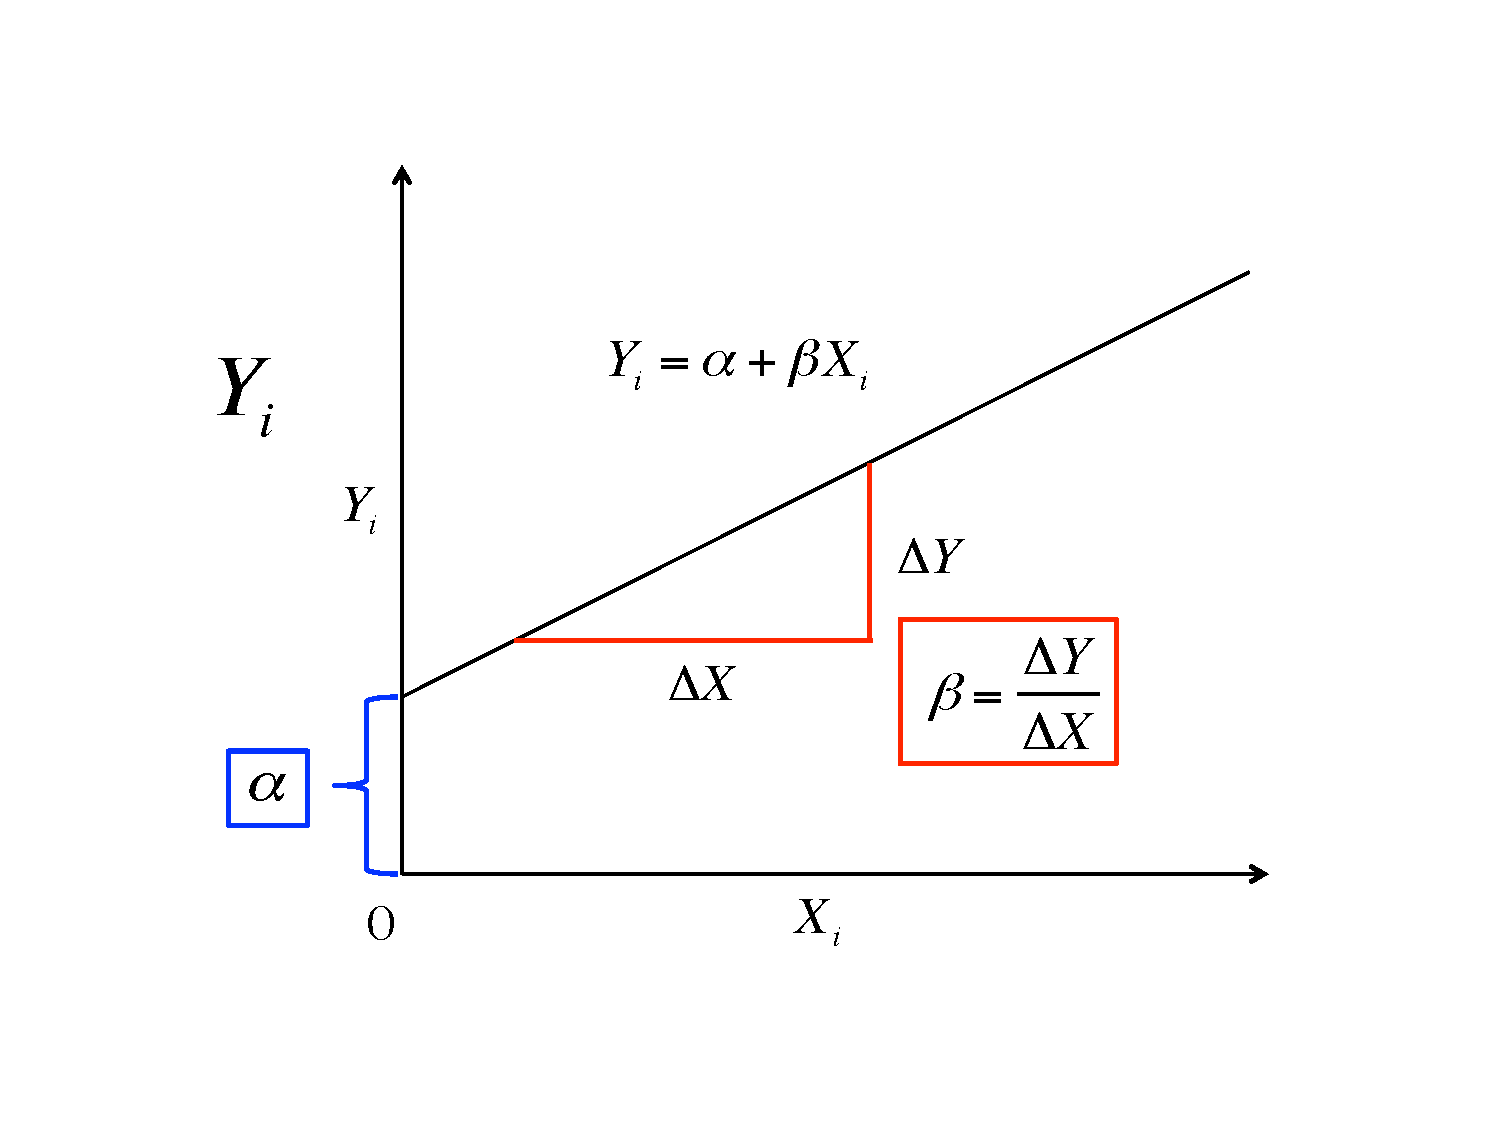
\includegraphics[width=4in]{07_OLSlogic/deterols.pdf}%filename
  \caption{Deterministic Model \label{dols}}  
\end{figure}

Given that in social science we rarely work with deterministic models, nearly all models contain a stochastic, or random, component. 

\subsection{Stochastic Linear Model} 

The stochastic, or statistical, linear model contains a systematic component, $Y = \alpha+\beta$, and a stochastic component called the \textbf{error term}. The error term is the difference between the expected value of $Y_i$ and the observed value of $Y_i$; $Y_i-\mu$. This model is expressed as: 

\begin{equation}
  \label{eq:theolm}
Y_{i} = \alpha + \beta X_{i} + \epsilon_i
\end{equation}

\noindent where $\epsilon_i$ is the error term. In the deterministic model, each value of $Y$ fits along the regression line, however in a stochastic model the expected value of $Y$ is conditioned by the values of $X$. This is illustrated in Figure \ref{sols}. 



\begin{figure}
  \centering
  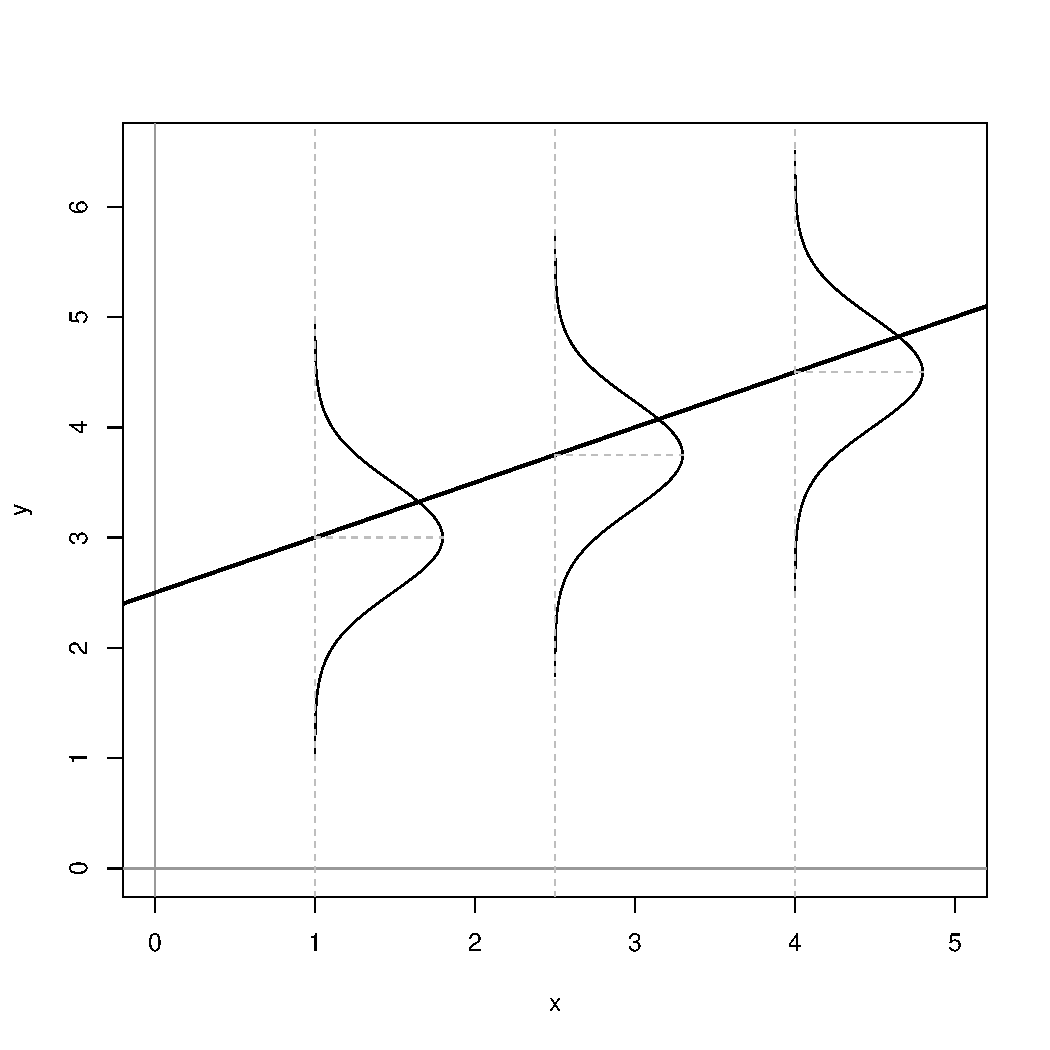
\includegraphics[width=4in]{07_OLSlogic/stochastic.pdf}%filename
  \caption{Stochastic Linear Model \label{sols}}
\end{figure}

Figure \ref{sols} shows the conditional population distributions of $Y$ for several values of $X, p(Y|X)$. The conditional means of $Y$ given $X$ are denoted $\mu$.  

\begin{equation} 
\mu_{i} \equiv E(Y_{i}) \equiv E(Y|X_{i})=\alpha+\beta X_{i} 
\end{equation} 
\noindent where 
\begin{itemize}
\item $\alpha = E(Y) \equiv \mu$ when $X=0$
\item Each 1 unit increase in $X$ increases $E(Y)$ by $\beta$
\end{itemize}

However, in the stochastic linear model variation in $Y$ is caused by more than $X$, it is also caused by the error term $\epsilon$.   The error term is expressed as: 

\begin{align*}
\epsilon_i &= Y_{i}-E(Y_{i}) \\
&= Y_{i}-(\alpha+\beta X_{i}) \\
&= Y_{i}-\alpha-\beta X_{i}
\end{align*}
Therefore;
\begin{align*}
Y_{i} &= E(Y_{i})+\epsilon \\
&= \alpha+\beta X_{i}+\epsilon_{i} 
\end{align*}
\noindent We make several important assumptions about the error term that are discussed in the next section. 

\subsubsection{Assumptions about the Error Term} 

There are three key assumptions about the error term; a) errors have identical distributions, b) errors are independent, c) errors are normally distributed.\footnote{Actually, we assume only that the \textbf{means} of the errors drawn from repeated samples of observations will be normally distributed -- but we will deal with that wrinkle later on.}

\begin{grbox}
\greybox{\textbf{Error Assumptions}
  \begin{enumerate}  
\item Errors have identical distributions
  \begin{center}
    $E(\epsilon^{2}_{i}) = \sigma^2_{\epsilon}$
  \end{center}
\item Errors are independent of $X$ and other $\epsilon_{i}$
  \begin{center}
    $E(\epsilon_{i}) \equiv E(\epsilon|x_{i}) = 0$ 
    
    and 
    
    $E(\epsilon_{i}) \neq E(\epsilon_{j})$ for $i \neq j$
  \end{center}
\item Errors are normally distributed
  \begin{center}
    $\epsilon_{i} \sim N(0,\sigma^2_{\epsilon})$
  \end{center}
\end{enumerate}}
\end{grbox}

Taken together these assumption mean that the error term has a normal, independent, and identical distribution (normal i.i.d.). However, we don't know if, in any particular case, these assumptions are met. Therefore we must estimate a linear model. 

\section{Estimating Linear Models} 

With stochastic models we don't know if the error assumptions are met, nor do we know the values of $\alpha$ and $\beta$ therefore we must estimate them, as denoted by a hat (e.g., $\hat{\alpha}$ is the estimate for $\alpha$). The stochastic model as shown in Equation \ref{eq:lm} is estimated as: 
\begin{equation}
  \label{eq:lm}
Y_{i} = \hat{\alpha} + \hat{\beta} X_{i}+ \epsilon_{i} 
\end{equation}
\noindent where $\epsilon_i$ is the \textbf{residual term}, or the estimated error term. Since no line can perfectly pass through all the data points, we introduce a residual, $\epsilon$, into the regression equation. Note that the predicted value of $Y$ is denoted $\hat{Y}$; $y$-hat. 

\begin{align*}
Y_{i} &= \hat{\alpha}+\hat{\beta}X_{i}+\epsilon_{i} \\ 
&= \hat{Y_{i}} + \epsilon_{i}  \\
\epsilon_{i} &= Y_i-\hat{Y_{i}} \\
&= Y_i-\hat{\alpha}-\hat{\beta}X_i
\end{align*}

\subsection{Residuals}
Residuals measure prediction errors, of how far observation $Y_{i}$ is from predicted $\hat{Y_{i}}$. This is shown in Figure \ref{resid}. 

\begin{figure}
  \centering
  \includegraphics[width=4in]%
    {07_OLSlogic/resids.pdf}% picture filename
  \caption{Residuals: Statistical Forensics \label{resid}}
\end{figure}

%what's in \epislon
The residual term contains the accumulation (sum) of errors that can result from measurement issues, modeling problems, and irreducible randomness. Ideally, the residual term contains lots of small and independent influences that result in an overall random quality of the distribution of the errors. When that distribution is not random -- that is, when the distribution of error has some systematic quality -- the estimates of $\hat{\alpha}$ and $\hat{\beta}$ may be biased. Thus, when we evaluate our models we will focus on the \texttt{shape} of the distribution of our errors. 

\begin{grbox}
\greybox{\textbf{What's in $\epsilon$?} 

  \textit{Measurement Error}
\begin{itemize}
\item Imperfect operationalizations
\item Imperfect measure application
\end{itemize}

\textit{Modeling Error}
\begin{itemize}
\item Modeling error/mis-specification
\item Missing model explanation
\item Incorrect assumptions about associations
\item Incorrect assumptions about distributions
\end{itemize}

\textit{Stochastic "noise"}
\begin{itemize}
\item Unpredictable variability in the dependent variable

\end{itemize}}
\end{grbox}

The goal of regression analysis is to minimize the error associated with the model estimates. As noted, the residual term is the estimated error, or overall ``miss" (e.g., $Y_{i}-\hat{Y_{i}}$). Specifically the goal is to minimize the sum of the squared errors, $\sum \epsilon^{2}$. Therefore, we need to find the values of $\hat{\alpha}$ and $\hat{\beta}$ that minimize $\sum \epsilon^{2}$. 

Note that for a fixed set of data \{$\hat{\alpha}$,$\hat{\alpha}$\}, each possible choice of values for $\hat{\alpha}$ and $\hat{\beta}$ corresponds to a specific residual sum of squares, $\sum \epsilon^{2}$. This can be expressed by the following functional form:

\begin{equation}
 S(\hat{\alpha},\hat{\beta})=\sum_{i=1}^{n} \epsilon^{2}_{i}=\sum (Y_{i}-\hat{Y_{i}})^{2}=\sum (Y_{i}-\hat{\alpha}-\hat{\beta}X_{i})^{2}  
\end{equation}

Minimizing this function requires specifying estimators for $\hat{\alpha}$ and $\hat{\beta}$ such that $S(\hat{\alpha},\hat{\beta})=\sum \epsilon^{2}$ is at the lowest possible value. Finding this minimum value requires the use of calculus, which will be discussed in the next chapter. Before that we walk through a quick example of simple regression.  

\section{An Example of Simple Regression} 

The following example uses a measure of peoples' political ideology to predict their perceptions of the risks posed by global climate change. OLS regression can be done using the \texttt{lm} function in \texttt{R}. For this example, we are using the \texttt{tbur} data set. 

\begin{knitrout}
\definecolor{shadecolor}{rgb}{0.969, 0.969, 0.969}\color{fgcolor}\begin{kframe}
\begin{alltt}
\hlstd{ols1} \hlkwb{<-} \hlkwd{lm}\hlstd{(ds}\hlopt{$}\hlstd{glbcc_risk} \hlopt{~} \hlstd{ds}\hlopt{$}\hlstd{ideol)}
\hlkwd{summary}\hlstd{(ols1)}
\end{alltt}
\begin{verbatim}
## 
## Call:
## lm(formula = ds$glbcc_risk ~ ds$ideol)
## 
## Residuals:
##    Min     1Q Median     3Q    Max 
## -8.726 -1.633  0.274  1.459  6.506 
## 
## Coefficients:
##             Estimate Std. Error t value            Pr(>|t|)    
## (Intercept) 10.81866    0.14189   76.25 <0.0000000000000002 ***
## ds$ideol    -1.04635    0.02856  -36.63 <0.0000000000000002 ***
## ---
## Signif. codes:  0 '***' 0.001 '**' 0.01 '*' 0.05 '.' 0.1 ' ' 1
## 
## Residual standard error: 2.479 on 2511 degrees of freedom
##   (34 observations deleted due to missingness)
## Multiple R-squared:  0.3483,	Adjusted R-squared:  0.348 
## F-statistic:  1342 on 1 and 2511 DF,  p-value: < 0.00000000000000022
\end{verbatim}
\end{kframe}
\end{knitrout}

The output in R provides a quite a lot of information about the relationship between the measures of ideology and perceived risks of climate change. It provides an overview of the distribution of the residuals; the estimated coefficients for $\hat{\alpha}$ and $\hat{\beta}$; the results of hypothesis tests; and overall measures of model ``fit" -- all of which we will discuss in detail in later chapters. But, for now, note that the estimated $B$ for ideology is negative, which indicates that as the value for ideology \textit{increases}---in our data this means more conservative---the perceived risk of climate change \textit{decreases}. Specifically, for each one unit increase in the ideology scale, perceived climate change risk decreases by -1.0463463.

We can also examine the distribution of the residuals, using a histogram and a density curve. This is shown in Figure \ref{fig:resid}. Note that we will discuss residual diagnostics in detail in future chapters. 

\begin{knitrout}
\definecolor{shadecolor}{rgb}{0.969, 0.969, 0.969}\color{fgcolor}\begin{kframe}
\begin{alltt}
\hlkwd{data.frame}\hlstd{(ols1}\hlopt{$}\hlstd{residuals)} \hlopt \hlkwd{ggplot}\hlstd{(}\hlkwd{aes}\hlstd{(ols1}\hlopt{$}\hlstd{residuals))} \hlopt{+}
    \hlkwd{geom_histogram}\hlstd{(}\hlkwc{bins} \hlstd{=} \hlnum{16}\hlstd{)}
\hlkwd{data.frame}\hlstd{(ols1}\hlopt{$}\hlstd{residuals)} \hlopt \hlkwd{ggplot}\hlstd{(}\hlkwd{aes}\hlstd{(ols1}\hlopt{$}\hlstd{residuals))} \hlopt{+}
    \hlkwd{geom_density}\hlstd{(}\hlkwc{adjust} \hlstd{=} \hlnum{1.5}\hlstd{)}
\hlkwd{dev.off}\hlstd{()}
\end{alltt}
\end{kframe}
\end{knitrout}
 
\begin{figure}
        \centering
        \begin{subfigure}[b]{0.4\textwidth}
                \centering
                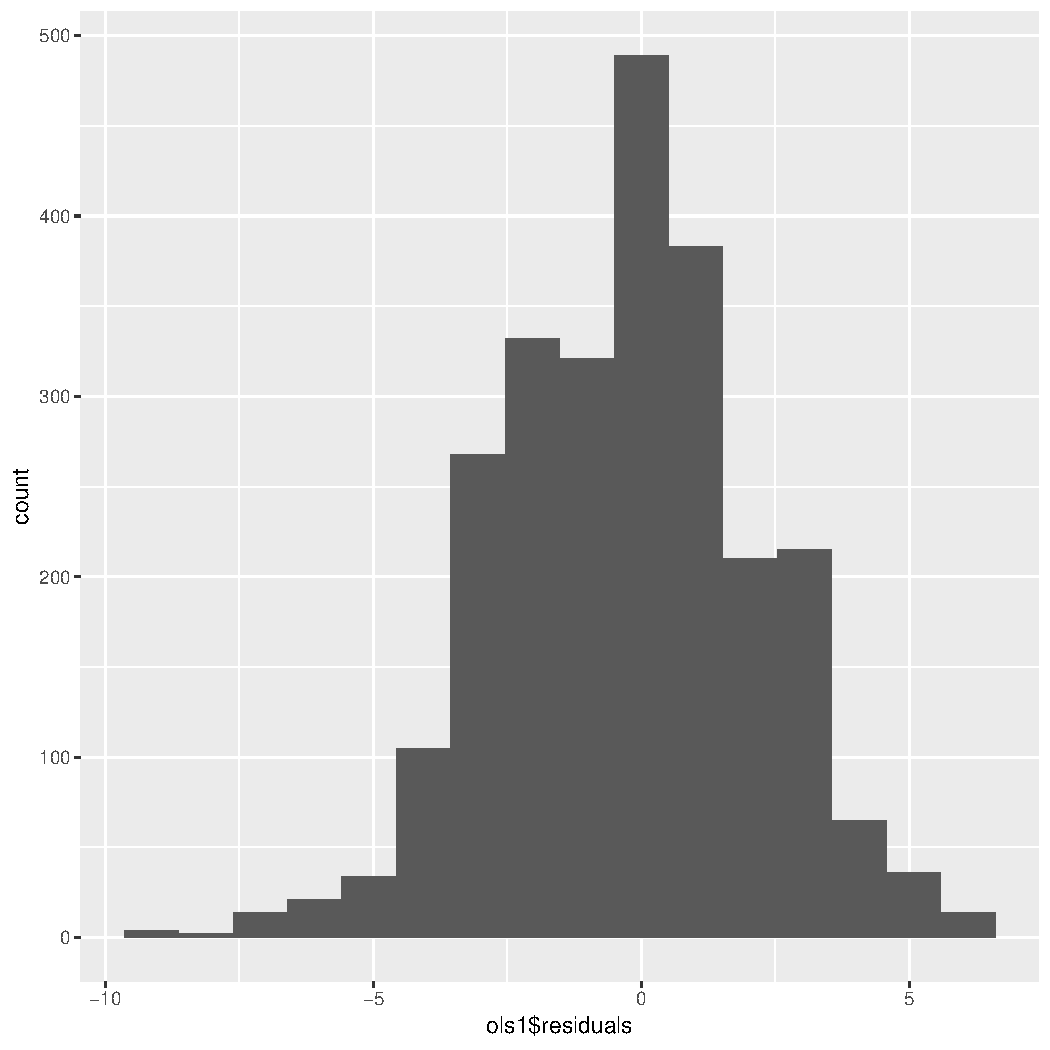
\includegraphics[width=\textwidth]{07_OLSlogic/exresidhist.pdf}%filename
                \caption{Histogram}
        \end{subfigure}
        \begin{subfigure}[b]{0.4\textwidth}
                \centering
                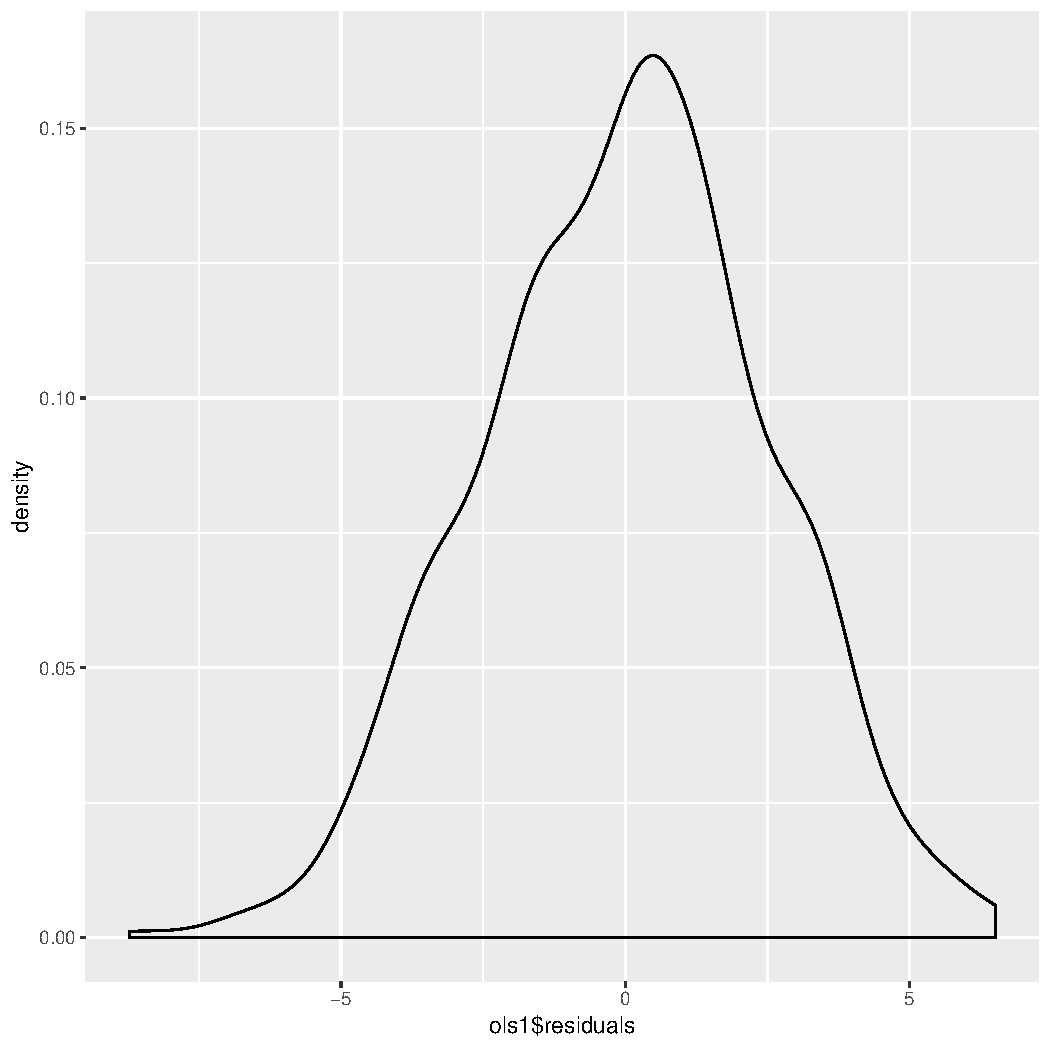
\includegraphics[width=\textwidth]{07_OLSlogic/exresidden.pdf}%filename
                \caption{Density}
        \end{subfigure}
        \caption{Residuals of Simple Regression Example \label{fig:resid}} 
\end{figure}        
\FloatBarrier

For purposes of this Chapter, be sure that you can run the basic bivariate OLS regression model in \textit{R}. If you can -- congratulations! If not, try again. And again. And again...




\chapter{Linear Estimation and Minimizing Error} 

As noted in the last chapter, the objective when estimating a linear model is to minimize the aggregate of the squared error. Specifically, when estimating a linear model, $Y=A+BX+E$, we seek to find the values of $\hat{\alpha}$ and $\hat{\beta}$ that minimize the $\sum \epsilon^{2}$. To accomplish this, we use calculus. 

\section{Minimizing Error using Derivatives}

In calculus, the \textit{derivative} is a measure the slope of any function of x, or $f(x)$, at each given value of $x$. For the function $f(x)$, the derivative is denoted as $f'(x)$ or, pronounced as \textit{``f prime x"}. Because the formula for $\sum \epsilon^{2}$ is known, and can be treated as a function, the derivative of that function permits the calculation of the change in the sum of the squared error over each possible value of $\hat{\alpha}$ and $\hat{\beta}$. For that reason we need to find the derivative for $\sum \epsilon^{2}$ with respect to changes in $\hat{\alpha}$ and $\hat{\beta}$. That, in turn, will permit us to ``derive" the values of $\hat{\alpha}$ and $\hat{\beta}$ that result in the lowest possible $\sum \epsilon^{2}$.

Look -- we understand that all this sounds complicated. But it's not all \textit{that} complicated. In this chapter we will walk through all the steps so you'll see that its really rather simple and, well, elegant. You will see that differential calculus (the kind of calculus that is concerned with rates of change) is built on a set of clearly defined rules for finding the derivative for any function $f(x)$. It's like solving a puzzle. The next section outlines these rules, so we can start solving puzzles. 

\subsection{Rules of Derivation} 

\begin{grbox}
\greybox{\textbf{Derivative Rules}
\begin{enumerate}  
\item Power Rule % 1
  \begin{center}
    If $f(x)=x^{n}$ then $f'(x)=n*x^{n-1}$
  \end{center}
\item Constant Rule % 2
  \begin{center}
    If $f(x)=c$ then $f'(x)=0$
  \end{center}
\item A Constant Times a Function % 3
  \begin{center}
    If $f(x)=c*u(x)$ then $f'(x)=c*u'(x)$
  \end{center}
\item Differentiating a Sum % 4
  \begin{center}
    If $f(x)=u(x)+v(x)$ then $f'(x)=u'(x)+v'(x)$
  \end{center}
\item Product Rule % 5
  \begin{center}
    If $f(x)=u(x)*v(x)$ then $f'(x)=u'(x)*v(x)+u(x)*v'(x)$
  \end{center}
\item Quotient Rule % 6
  \begin{center}
    If $f(x)=\frac{N(x)}{D(x)}$ then 
    $f'(x)=\frac{D(x)*N'(x)-D'(x)*N(x)}{[D(x)]^{2}}$
  \end{center}
\item Chain Rule % 7
  \begin{center}
   If $f(x)=[u(x)]^{n}$ then $f'(x)=n*[u(x)]^{n-1}*u'(x)$ 
  \end{center}
\end{enumerate}}
\end{grbox}

The following sections provide examples of the application of each rule. 

\subsubsection{\textit{Rule 1: the Power Rule}}

\begin{center}
    If $f(x)=x^{n}$ then $f'(x)=n*x^{n-1}$
  \end{center}
  \noindent 
Example: 
\begin{align*}  
 f(x) &= x^{6} \\ 
 f'(x) &= 6*x^{6-1} \\
 &=6x^{5} 
\end{align*}

A second example can be plotted in \texttt{R}. The function is $f(x)=x^{2}$ and therefore, using the power rule, the derivative is: $f'(x)=2x$. 

\begin{knitrout}
\definecolor{shadecolor}{rgb}{0.969, 0.969, 0.969}\color{fgcolor}\begin{kframe}
\begin{alltt}
\hlstd{x} \hlkwb{<-} \hlkwd{c}\hlstd{(}\hlopt{-}\hlnum{5}\hlopt{:}\hlnum{5}\hlstd{)}
\hlstd{x}
\hlstd{y} \hlkwb{<-} \hlstd{x}\hlopt{^}\hlnum{2}
\hlstd{y}
\end{alltt}
\end{kframe}
\end{knitrout}

\begin{figure}
  \centering
  \includegraphics[width=0.6\textwidth]%
    {08_Derivatives/powerfun.pdf}% picture filename
  \caption{Calculating Slopes for $(x,y)$ Pairs \label{fig:powerfun}}
\end{figure}
\FloatBarrier

\subsubsection{\textit{Rule 2: the Constant Rule}}

\begin{center}
    If $f(x)=c$ then $f'(x)=0$
  \end{center}
\noindent Example: 
\begin{align*}
f(x) &=346 \\ 
f'(x)&=0 \\
&=10x
\end{align*}

\subsubsection{\textit{Rule 3: a Constant Times a Function}}

  \begin{center}
    If $f(x)=c*u(x)$ then $f'(x)=c*u'(x)$
  \end{center}
\noindent Example:
\begin{align*}
f(x) &= 5x^{2} \\ 
f'(x)&=5*2x^{2-1} \\
&=10x
\end{align*}

\subsubsection{\textit{Rule 4: Differentiating a Sum}}

  \begin{center}
    If $f(x)=u(x)+v(x)$ then $f'(x)=u'(x)+v'(x)$
  \end{center}
\noindent Example:  
\begin{align*}
f(x)&= 4x^{2}+32x \\
f'(x)&=(4x^{2})'+(32x)' \\
&=4*2x^{2-1}+32 \\
&=8x+32 
\end{align*}

\subsubsection{\textit{Rule 5: the Product Rule}}

  \begin{center}
    If $f(x)=u(x)*v(x)$ then $f'(x)=u'(x)*v(x)+u(x)*v'(x)$
  \end{center}
\noindent Example: 
\begin{align*}
f(x) &= x^{3}(x-5) \\ 
f'(x)&=(x^{3})'(x-5)+(x^{3})(x-5)' \\
&=3x^{2}(x-5)+(x^{3})*1 \\
&=3x^{3}-15x^{2}+x^{3}\\
&=4x^{3}-15x^{2} 
\end{align*}

In a second example, the product rule is applied the function $y=f(x)=x^{2}-6x+5$. The derivative of this function is $f'(x)=2x-6$. This function can be plotted in \texttt{R}.  

\begin{knitrout}
\definecolor{shadecolor}{rgb}{0.969, 0.969, 0.969}\color{fgcolor}\begin{kframe}
\begin{alltt}
\hlstd{x} \hlkwb{<-} \hlkwd{c}\hlstd{(}\hlopt{-}\hlnum{1}\hlopt{:}\hlnum{7}\hlstd{)}
\hlstd{x}
\hlstd{y} \hlkwb{<-} \hlstd{x}\hlopt{^}\hlnum{2} \hlopt{-} \hlnum{6} \hlopt{*} \hlstd{x} \hlopt{+} \hlnum{5}
\hlstd{y}
\hlkwd{plot}\hlstd{(x, y,} \hlkwc{type} \hlstd{=} \hlstr{"o"}\hlstd{,} \hlkwc{pch} \hlstd{=} \hlnum{19}\hlstd{)}
\hlkwd{abline}\hlstd{(}\hlkwc{h} \hlstd{=} \hlnum{0}\hlstd{,} \hlkwc{v} \hlstd{=} \hlnum{0}\hlstd{)}
\end{alltt}
\end{kframe}
\end{knitrout}

\begin{figure}
  \centering
  \includegraphics[width=0.6\textwidth]%
    {08_Derivatives/powerfun.pdf}% picture filename
  \caption{Plot of Function $y=f(x)=x^2-6x+5$ \label{fig:prodfun}}
\end{figure}
\FloatBarrier

\noindent We can also use the derivative and \texttt{R} to calculate the slope for each value of $X$. 

\begin{knitrout}
\definecolor{shadecolor}{rgb}{0.969, 0.969, 0.969}\color{fgcolor}\begin{kframe}
\begin{alltt}
\hlstd{b} \hlkwb{<-} \hlnum{2} \hlopt{*} \hlstd{x} \hlopt{-} \hlnum{6}
\hlstd{b}
\end{alltt}
\begin{verbatim}
## [1] -8 -6 -4 -2  0  2  4  6  8
\end{verbatim}
\end{kframe}
\end{knitrout}

The values for $X$, which as shown in Figure \ref{fig:prodfun} range from -8 to +8, return derivatives (slopes at a point) ranging from -25 to +25.

\subsubsection{\textit{Rule 6: the Quotient Rule}}
 
 \begin{center}
    If $f(x)=\frac{N(x)}{D(x)}$ then 
    $f'(x)=\frac{D(x)*N'(x)-D'(x)*N(x)}{[D(x)]^{2}}$
  \end{center}
\noindent Example: 
\begin{align*}
f(x) &=\frac{x}{x^{2}+5} \\
f'(x)&=\frac{(x^{2}+5)(x)'-(x^{2}+5)'(x)}{(x^{2}+5)^{2}} \\
&=\frac{(x^{2}+5)-(2x)(x)}{(x^{2}+5)^{2}} \\
&= \frac{-x^{2}+5}{(x^{2}+5)^{2}}   
\end{align*}

\subsubsection{\textit{Rule 7: the Chain Rule}}

\begin{center}
   If $f(x)=[u(x)]^{n}$ then $f'(x)=n*[u(x)]^{n-1}*u'(x)$ 
  \end{center}
\noindent Example: 
\begin{align*}
f(x) &= (7x^{2}-2x+13)^{5} \\ 
f'(x)&=5(7x^{2}-2x+13)^{4}*(7x^{2}-2x+13)' \\
&=5(7x^{2}-2x+13)^{4}*(14x-2)
\end{align*}

\subsection{Critical Points}

Our goal is to use derivatives to find the values of $\hat{\alpha}$ and $\hat{\beta}$ that minimize the sum of the squared error. To do this we need to find the \textit{minima} of a function. The minima is the smallest value that a function takes, whereas the maxima is the largest value. To find the minima and maxima, the \textit{critical points} are key. The critical point is where the derivative of the function is equal to $0$, $f'(x)=0$. Note, that this is equivalent to the slope being equal to $0$. 

\begin{grbox}
\greybox{{\textbf{Example: Finding the Critical Points}}

To find the critical point for the function $y=f(x)=(x^{2}-4x+5)$;
\begin{itemize}
  \item First find the derivative; $f'(x)=2x-4$ 
  \item Set the derivative equal to $0$; $f'(x)=2x-4=0$ 
  \item Solve for $x$; $x=2$ 
  \item Substitute $2$ for $x$ into the function and solve for $y$
    \begin{center}
      $y=f(2)=2^{2}-4(2)+5=1$ 
    \end{center}
 \item Thus, the critical point (there's only one in this case) of the function is $(2,1)$
\end{itemize}}   
\end{grbox}

Once a critical point is identified, the next step is to determine whether that point is a minima or a maxima. The most straight forward way to do this is to identify the x,y coordinates and plot. This can be done in \texttt{R}, as we will show using the function $y=f(x)=(x^{2}-4x+5)$. The plot is shown in Figure \ref{fig:crit}. 
\begin{knitrout}
\definecolor{shadecolor}{rgb}{0.969, 0.969, 0.969}\color{fgcolor}\begin{kframe}
\begin{alltt}
\hlstd{x} \hlkwb{<-} \hlkwd{c}\hlstd{(}\hlopt{-}\hlnum{5}\hlopt{:}\hlnum{5}\hlstd{)}
\hlstd{x}
\hlstd{y} \hlkwb{<-} \hlstd{x}\hlopt{^}\hlnum{2} \hlopt{-} \hlnum{4} \hlopt{*} \hlstd{x} \hlopt{+} \hlnum{5}
\hlstd{y}
\end{alltt}
\end{kframe}
\end{knitrout}

\begin{figure}[h]
  \centering
  \includegraphics[width=0.4\textwidth]%
    {08_Derivatives/crit.pdf}% picture filename
  \caption{Identification of Critical Points \label{fig:crit}}
\end{figure}
\FloatBarrier

\noindent As can be seen, the critical point $(2,1)$ is a minima. 

\subsection{Partial Derivation}

When an equation includes two variables, one can take a \textit{partial derivative} with respect to only one variable while the other variable is simply treated as a constant. This is particularly useful in our case, because the function $\sum \epsilon^{2}$ has two variables -- $\hat{\alpha}$ and ${\hat{\beta}$.

Let's take an example. For the function $y=f(x,z)=x^{3}+4xz-5z^{2}$, we first take the derivative of $x$ holding $z$ constant. 

\begin{align*}
 \frac{\partial y}{\partial x} &= \frac{\partial f(x,z)}{\partial x} \\
 &= 3x^{2}+4z
\end{align*}
Next we take the derivative of $z$ holding $x$ constant. 
\begin{align*}
 \frac{\partial y}{\partial z} &= \frac{\partial f(x,z)}{\partial z} \\
 &= 4x-10z
\end{align*}

\section{Deriving OLS Estimators}

Now that we have developed some of the rules for differential calculus, we can see how OLS finds values of $\hat{\alpha}$ and $\hat{\beta}$ that minimizes the sum of the squared error. In formal terms, let's define the set, $S(\hat{\alpha},\hat{\beta})$ as a pair of regression estimators that jointly determine the residual sum of squares given that: $Y_{i}=\hat {Y}_{i}+\epsilon_{i}=\hat{\alpha}+\hat{\beta}X_{i}+\epsilon_{i}$. This function can be expressed:

\begin{equation*}
 S(\hat{\alpha},\hat{\beta})=\sum_{i=1}^{n} \epsilon^{2}_{i}=\sum (Y_{i}-\hat{Y_{i}})^{2}=\sum (Y_{i}-\hat{\alpha}-\hat{\beta} X_{i})^{2}  
\end{equation*}
First we will derive $\hat{\alpha}$. 

\subsection{OLS Derivation of $\hat{\alpha}$}

Take the partial derivatives of $S(\hat{\alpha},\hat{\beta})$ with-respect-to (w.r.t) $\hat{\alpha}$ in order to determine the formulation of $\hat{\alpha}$ that minimizes $S(\hat{\alpha},\hat{\beta})$. Using the chain rule,

\begin{align*}
\frac{\partial S(\hat{\alpha},\hat{\beta})}{\partial \hat{\alpha}} &= \sum
2(Y_{i}-\hat{\alpha}-\hat{\beta}X_{i})^{2-1}*(Y_{i}-\hat{\alpha}-\hat{\beta}X_{i})' \\
&= \sum 2(Y_{i}-\hat{\alpha}-\hat{\beta}X_{i})^{1}*(-1) \\
&= -2 \sum (Y_{i}-\hat{\alpha}-\hat{\beta}X_{i}) \\ 
&= -2 \sum Y_{i}+2n\hat{\alpha}+2\hat{\beta} \sum X_{i} 
\end{align*}

\noindent Next set the derivative equal to $0$. 

\begin{equation*}
\frac{\partial S(\hat{\alpha},\hat{\beta})}{\partial \hat{\alpha}} =  -2 \sum Y_{i}+2n\hat{\alpha}+2\hat{\beta} \sum X_{i} = 0 
\end{equation*}

\noindent Then, shift non-$\hat{\alpha}$ terms to the other side of the equal sign:
\begin{equation*}
2n\hat{\alpha} = 2 \sum Y_{i}-2\hat{\beta} \sum X_{i} 
\end{equation*}

\noindent Finally, divide through by $2n$: 
\begin{align*}
\frac{2n\hat{\alpha}}{2n} &= \frac{2 \sum Y_{i}-2\hat{\beta} \sum X_{i}}{2n} \\
A &= \frac{\sum Y_{i}}{n}-\hat{\beta}*\frac{\sum X_{i}}{n} \\
&= \bar {Y}-\hat{\beta} \bar{X} \\
\end{align*}

\begin{equation}
\label{eq:A} 
\therefore \hat{\alpha} = \bar {Y}-\hat{\beta} \bar{X} 
\end{equation}


\subsection{OLS Derivation of $\hat{\beta}$}

Having found $\hat{\alpha}$, the next step is to derive $\hat{\beta}$. This time we will take the partial derivative w.r.t $\hat{\beta}$. As you will see, the steps are just a little more involved for $\hat{\beta}$ than they were for $\hat{\alpha}$.

\begin{align*}
\frac{\partial S(\hat{\alpha},\hat{\beta})}{\partial \hat{\beta}} &= \sum
2(Y_{i}-\hat{\alpha}-\hat{\beta}X_{i})^{2-1}*(Y_{i}-\hat{\alpha}-\hat{\beta}X_{i})' \\
&= \sum 2(Y_{i}-\hat{\alpha}-\hat{\beta}X_{i})^{1}*(-X_{i}) \\
&= 2 \sum (-X_{i}Y_{i}+\hat{\alpha}X_{i}+\hat{\beta}X^{2}_{i}) \\ 
&= -2 \sum X_{i}Y_{i}+2\hat{\alpha} \sum X_{i} + 2\hat{\beta} \sum X^{2}_{i}  
\end{align*}

\noindent Since we know that $\hat{\alpha} = \bar {Y}-\hat{\beta} \bar{X}$, we can substitute $\bar {Y}-\hat{\beta}
\bar{X}$ for $\hat{\alpha}$. 

\begin{align*}
\frac{\partial S(\hat{\alpha},\hat{\beta})}{\partial \hat{\beta}} &= -2 \sum X_{i}Y_{i}+2(\bar {Y}-\hat{\beta}
\bar{X})\sum X_{i} + 2\hat{\beta} \sum X^{2}_{i} \\
&= -2 \sum X_{i}Y_{i}+2 \bar{Y} \sum X_{i}-2\hat{\beta} \bar{X} \sum X_{i} + 2\hat{\beta}
\sum X^{2}_{i} 
\end{align*}

\noindent Next, we can substitute $\frac{\sum Y_{i}}{n}$ for $\bar{Y}$ and $\frac{\sum X_{i}}{n}$ for $\bar{X}$ and set it equal to $0$. 

\begin{equation*}
\frac{\partial S(\hat{\alpha},\hat{\beta})}{\partial \hat{\beta}} = -2 \sum X_{i}Y_{i}+\frac{2\sum Y_{i}
  \sum X_{i}}{n}-\frac{2\hat{\beta}\sum X_{i} \sum X_{i}}{n}+ 2\hat{\beta}
\sum X^{2}_{i} = 0
\end{equation*}

\noindent Then, multiply through by $\frac{n}{2}$ and put all the $\hat{\beta}$ terms on the same side. 

\begin{align*}
n\hat{\beta} \sum X^{2}_{i}-\hat{\beta}(\sum X_{i})^{2} &= n \sum X_{i}Y_{i}-\sum X_{i}
\sum Y_{i} \\
\hat{\beta}(n \sum X^{2}_{i}-(\sum X_{i})^{2}) &= n \sum X_{i}Y_{i}-\sum X_{i}
\sum Y_{i} \\
\therefore \hat{\beta} = \frac{n \sum X_{i}Y_{i}-\sum X_{i}
\sum Y_{i}}{n\sum X^{2}_{i}-(\sum X_{i})^{2}}
\end{align*}

\noindent The $\hat{\beta}$ term can be rearranged such that: 

\begin{equation}
\label{eq:B}  
\hat{\beta}=\frac{\Sigma(X_{i}-\bar X)(Y_{i}-\bar Y)}{\Sigma(X_{i}-\bar X)^2}  
\end{equation}

Now remember what we are doing here: We used the partial derivatives for $\sum \epsilon^{2}$ with respect to $\hat{\alpha}$ and $\hat{\beta}$ to find the values for $\hat{\alpha}$ and $\hat{\beta}$ that will give us the smallest value for $\sum \epsilon^{2}$.  Put differently, the formulas for $\hat{\beta}$ and $\hat{\alpha}$ allow the calculation of the error-minimizing slope (change in $Y$ given a one unit change in $X$) and intercept (value for $Y$ when $X$ is zero) for any data set representing a bivariate, linear relationship. No other formulas will give us a line, using the same data, that will result in as small a squared-error. Therefore, OLS is referred to as the Best Linear Unbiased Estimator (BLUE).  

\subsection{Interpreting $\hat{\beta}$ and $\hat{\alpha}$}

In a regression equation $Y=\hat{\alpha}+\hat{\beta}X$, where $\hat{\alpha}$ is shown in Equation \ref{eq:A} and $\hat{\beta}$ is shown in Equation \ref{eq:B}. Equation \ref{eq:B} shows that for each 1-unit increase in $X$ you get $\hat{\beta}$ units change in $Y$. Equation \ref{eq:A} shows that when $X$ is $0$, $Y$ is equal to $\hat{\alpha}$. Note that in a regression model with no independent variables, $\hat{\alpha}$ is simply the expected value (i.e., mean) of $Y$. 

The intuition behind these formulas can be shown by using \texttt{R} to calculate ``by hand" the slope ($\hat{\beta}$) and intercept ($\hat{\alpha}$) coefficients. A theoretical simple regression model is structured as
follows:  

\begin{equation*}
Y_{i} = \alpha + \beta X_{i} + \epsilon_{i} 
\end{equation*}

\begin{itemize}
\item $\alpha$ and $\beta$ are constant terms
\item $\alpha$ is the intercept
\item $\beta$ is the slope
\item $X_{i}$ is a predictor of $Y_{i}$
\item $\epsilon$ is the error term
\end{itemize}

\noindent The model is to be estimated is expressed as $Y=\hat{\beta}+\hat{\beta}X+/epsilon$. 

\noindent As noted, the goal is to calculate the intercept coefficient: 

\begin{equation*}
\hat{\alpha}=\bar Y-\hat{\beta}\bar X 
\end{equation*}

\noindent and the slope
coefficient: 
\begin{equation*}
\hat{\beta}=\frac{\Sigma(X_{i}-\bar X)(Y_{i}-\bar Y)}{\Sigma(X_{i}-\bar X)^2}
\end{equation*}

Using \texttt{R}, this can be accomplished in a few steps. First create a vector of values for \textit{x} and \textit{y} (note that we just chose these values arbitrarily for purposes of this example). 

\begin{knitrout}
\definecolor{shadecolor}{rgb}{0.969, 0.969, 0.969}\color{fgcolor}\begin{kframe}
\begin{alltt}
\hlstd{x} \hlkwb{<-} \hlkwd{c}\hlstd{(}\hlnum{4}\hlstd{,} \hlnum{2}\hlstd{,} \hlnum{4}\hlstd{,} \hlnum{3}\hlstd{,} \hlnum{5}\hlstd{,} \hlnum{7}\hlstd{,} \hlnum{4}\hlstd{,} \hlnum{9}\hlstd{)}
\hlstd{x}
\end{alltt}
\begin{verbatim}
## [1] 4 2 4 3 5 7 4 9
\end{verbatim}
\begin{alltt}
\hlstd{y} \hlkwb{<-} \hlkwd{c}\hlstd{(}\hlnum{2}\hlstd{,} \hlnum{1}\hlstd{,} \hlnum{5}\hlstd{,} \hlnum{3}\hlstd{,} \hlnum{6}\hlstd{,} \hlnum{4}\hlstd{,} \hlnum{2}\hlstd{,} \hlnum{7}\hlstd{)}
\hlstd{y}
\end{alltt}
\begin{verbatim}
## [1] 2 1 5 3 6 4 2 7
\end{verbatim}
\end{kframe}
\end{knitrout}

\noindent Then, create objects for $\bar {X}$ and $\bar {Y}$

\begin{knitrout}
\definecolor{shadecolor}{rgb}{0.969, 0.969, 0.969}\color{fgcolor}\begin{kframe}
\begin{alltt}
\hlstd{xbar} \hlkwb{<-} \hlkwd{mean}\hlstd{(x)}
\hlstd{xbar}
\end{alltt}
\begin{verbatim}
## [1] 4.75
\end{verbatim}
\begin{alltt}
\hlstd{ybar} \hlkwb{<-} \hlkwd{mean}\hlstd{(y)}
\hlstd{ybar}
\end{alltt}
\begin{verbatim}
## [1] 3.75
\end{verbatim}
\end{kframe}
\end{knitrout}

\noindent Next, create objects for $(X-\bar X)$ and $(Y-\bar Y)$, the deviations of $X$ and $Y$ around their means:

\begin{knitrout}
\definecolor{shadecolor}{rgb}{0.969, 0.969, 0.969}\color{fgcolor}\begin{kframe}
\begin{alltt}
\hlstd{x.m.xbar} \hlkwb{<-} \hlstd{x} \hlopt{-} \hlstd{xbar}
\hlstd{x.m.xbar}
\end{alltt}
\begin{verbatim}
## [1] -0.75 -2.75 -0.75 -1.75  0.25  2.25 -0.75  4.25
\end{verbatim}
\begin{alltt}
\hlstd{y.m.ybar} \hlkwb{<-} \hlstd{y} \hlopt{-} \hlstd{ybar}
\hlstd{y.m.ybar}
\end{alltt}
\begin{verbatim}
## [1] -1.75 -2.75  1.25 -0.75  2.25  0.25 -1.75  3.25
\end{verbatim}
\end{kframe}
\end{knitrout}

\noindent Then, calculate $\hat{\beta}$
\begin{equation*}
\hat{\beta}=\frac{\Sigma(X_{i}-\bar X)(Y_{i}-\bar Y)}{\Sigma(X_{i}-\bar X)^2}
\end{equation*}

\begin{knitrout}
\definecolor{shadecolor}{rgb}{0.969, 0.969, 0.969}\color{fgcolor}\begin{kframe}
\begin{alltt}
\hlstd{B} \hlkwb{<-} \hlkwd{sum}\hlstd{((x.m.xbar)} \hlopt{*} \hlstd{(y.m.ybar))}\hlopt{/}\hlkwd{sum}\hlstd{((x.m.xbar)}\hlopt{^}\hlnum{2}\hlstd{)}
\hlstd{B}
\end{alltt}
\begin{verbatim}
## [1] 0.7183099
\end{verbatim}
\end{kframe}
\end{knitrout}

\noindent Finally, calculate $\hat{\alpha}$
\begin{equation*}
\hat{\alpha}=\bar Y-\hat{\beta}\bar X 
\end{equation*}

\begin{knitrout}
\definecolor{shadecolor}{rgb}{0.969, 0.969, 0.969}\color{fgcolor}\begin{kframe}
\begin{alltt}
\hlstd{A} \hlkwb{<-} \hlstd{ybar} \hlopt{-} \hlstd{B} \hlopt{*} \hlstd{xbar}
\hlstd{A}
\end{alltt}
\begin{verbatim}
## [1] 0.3380282
\end{verbatim}
\end{kframe}
\end{knitrout}

\noindent To see the relationship, we can produce a scatterplot of \textit{x} and \textit{y} and then add our regression line, as shown in Figure \ref{fig:regex}. So, for each unit increase in $x$, $y$ increases by 0.7183099 and when $x$ is $0$, $y$ is equal to 0.3380282.  

\begin{knitrout}
\definecolor{shadecolor}{rgb}{0.969, 0.969, 0.969}\color{fgcolor}\begin{kframe}
\begin{alltt}
\hlkwd{plot}\hlstd{(x, y)}
\hlkwd{lines}\hlstd{(x, A} \hlopt{+} \hlstd{B} \hlopt{*} \hlstd{x)}
\end{alltt}
\end{kframe}
\end{knitrout}

\begin{figure}
  \centering
  \includegraphics[width=0.6\textwidth]%
    {08_Derivatives/regex.pdf}% picture filename
  \caption{Simple Regression of $x$ and $y$ \label{fig:regex}}
\end{figure}
\FloatBarrier

See figure \ref{fig:regex}.

\section{Summary}
Whoa! Think of what you've accomplished here: You learned enough calculus to find a minima for an equation with two variables, then applied that to the equation for the $\sum \epsilon^{2}$. You derived the error minimizing values for $\hat{\alpha}$ and $\hat{\beta}$. Then you used those formulae in $R$ to calculate ``by hand" the OLS regression for a small dataset. 

Congratulate yourself -- you deserve it!





\chapter{Bi-Variate Hypothesis Testing and Model Fit}

The previous chapters discussed the logic of OLS regression and how to derive OLS estimators. Now that simple regression is no longer a mystery, we will shift the focus to bi-variate hypothesis testing and model fit. Note that the examples in this chapter use the \texttt{tbur} data set.  We recommend that you try the analyses in the chapter as you read.

\section{Hypothesis Tests for Regression Coefficients}

Hypothesis testing is the key to theory building. This chapter is focused on empirical hypothesis testing using OLS regression, using examples drawn from the accompanying dataset (tbur.data). Here we will use the responses to the political ideology question  (ranging from 1=strong liberal, to 7=strong conservative), as well as responses to a question concerning the survey respondents' level of risk that global warming poses for people and the environment.\footnote{The question wording was as follows: ``On a scale from zero to ten, where zero
means no risk and ten means extreme risk, how much
risk do you think global warming poses for people
and the environment?"}

Using the data from these questions, we posit the following hypothesis:
\begin{quote}
$H_{1}$: On average, as respondents, become more politically conservative, they will be less likely to express increased risk associated with global warming.
\end{quote}

The null hypothesis, $H_{0}$, is $\beta = 0$, positing that a respondents ideology has no relationship with their views about the risks of global warming for people and the environment. Our working hypothesis, $H_{1}$, is $\beta < 0$. We expect $\beta$ to be less than zero because we expect a \textit{negative} slope between our measures of ideology and levels of risk associated with global warming, given that a larger numeric value for ideology indicates a more conservative respondent. Note that this is a \textit{directional} hypothesis since we are positing a negative relationship. Typically, a directional hypothesis implies a one-tailed test where the critical value is 0.05 on one side of the distribution. A \textit{non-directional} hypothesis, $\beta \neq 0$ does not imply a particular direction, it only implies that there is a relationship. This requires a two-tailed test where the critical value is 0.025 on both sides of the distribution.  

To test this hypothesis, we run the following code in \texttt{R}. 

Before we begin, for this chapter, we need to make a special data set that just contains the variables \texttt{glbccrisk} and \texttt{ideol} with missing values removed.

\begin{knitrout}
\definecolor{shadecolor}{rgb}{0.969, 0.969, 0.969}\color{fgcolor}\begin{kframe}
\begin{alltt}
\hlcom{# Filtering a data set with only variables glbcc_risk and}
\hlcom{# ideol}
\hlstd{ds.omit} \hlkwb{<-} \hlkwd{filter}\hlstd{(ds)} \hlopt \hlkwd{select}\hlstd{(glbcc_risk, ideol)} \hlopt \hlkwd{na.omit}\hlstd{()}
\hlcom{# Run the na.omit function to removed the value}
\end{alltt}
\end{kframe}
\end{knitrout}


\begin{knitrout}
\definecolor{shadecolor}{rgb}{0.969, 0.969, 0.969}\color{fgcolor}\begin{kframe}
\begin{alltt}
\hlstd{ols1} \hlkwb{<-} \hlkwd{lm}\hlstd{(glbcc_risk} \hlopt{~} \hlstd{ideol,} \hlkwc{data} \hlstd{= ds.omit)}
\hlkwd{summary}\hlstd{(ols1)}
\end{alltt}
\begin{verbatim}
## 
## Call:
## lm(formula = glbcc_risk ~ ideol, data = ds.omit)
## 
## Residuals:
##    Min     1Q Median     3Q    Max 
## -8.726 -1.633  0.274  1.459  6.506 
## 
## Coefficients:
##             Estimate Std. Error t value            Pr(>|t|)    
## (Intercept) 10.81866    0.14189   76.25 <0.0000000000000002 ***
## ideol       -1.04635    0.02856  -36.63 <0.0000000000000002 ***
## ---
## Signif. codes:  0 '***' 0.001 '**' 0.01 '*' 0.05 '.' 0.1 ' ' 1
## 
## Residual standard error: 2.479 on 2511 degrees of freedom
## Multiple R-squared:  0.3483,	Adjusted R-squared:  0.348 
## F-statistic:  1342 on 1 and 2511 DF,  p-value: < 0.00000000000000022
\end{verbatim}
\end{kframe}
\end{knitrout}

To know whether to accept of reject the null hypothesis, we need to first understand the standard error associated with the model and our coefficients. We start, therefore, with  consideration of the residual standard error of the regression model. 

\subsection{Residual Standard Error} 

The residual standard error (or standard error of the regression),  measures spread of our observations around the regression line. As will be discussed below, the residual standard error is used to calculate the standard errors of the regression coefficients, $A$ and $B$. 

The formula for the residual standard error is as follows:
\begin{equation}
S_{E}=\sqrt{\frac{\Sigma E^{2}_{i}}{n-2}}
\end{equation}

To calculate this in \texttt{R}, based on the model we just ran,  we create an object called \texttt{Se} and use the \texttt{sqrt} and \texttt{sum} commands. 
\begin{knitrout}
\definecolor{shadecolor}{rgb}{0.969, 0.969, 0.969}\color{fgcolor}\begin{kframe}
\begin{alltt}
\hlstd{Se} \hlkwb{<-} \hlkwd{sqrt}\hlstd{(}\hlkwd{sum}\hlstd{(ols1}\hlopt{$}\hlstd{residuals}\hlopt{^}\hlnum{2}\hlstd{)}\hlopt{/}\hlstd{(}\hlkwd{length}\hlstd{(ds.omit}\hlopt{$}\hlstd{glbcc_risk)} \hlopt{-}
    \hlnum{2}\hlstd{))}
\hlstd{Se}
\end{alltt}
\begin{verbatim}
## [1] 2.479022
\end{verbatim}
\end{kframe}
\end{knitrout}
\noindent Note that this result matches the result provided by the \texttt{summary} function in \texttt{R}, as shown above.  

For our model, the results indicate that: $Y_{i} =$ 10.8186624 -1.0463463$X_{i} + E_{i}$.  Another sample of 2513 observations would almost certainly lead to different estimates for $A$ and $B$.  If we drew many such samples, we’d get the sample distribution of the estimates. Because we typically cannot draw many samples, we need to estimate the sample distribution, based on our sample size and variance.  To do that, we calculate the standard error of the slope and intercept coefficients, $SE(B)$ and $SE(A)$. These standard errors are our estimates of how much variation we would expect in the estimates of $B$ and $A$ across different samples. We use them to evaluate whether $B$ and $A$ are larger that would be expected to occur by chance, if the real values of $B$ and/or $A$ are zero (the null hypotheses).

The standard error for $B$, $SE(B)$ is:
\begin{equation}
SE(B)=\frac{S_{E}}{\sqrt{TSS_{X}}}
\end{equation}
\noindent where $S_E$ is the residual standard error of the regression, (as whown earlier in equation 9.1). $TSS_X$ is the total sum of squares for $X$, that is the total sum of the squared deviations (residuals) of $X$ from its mean $\bar{X}$; $\sum (X_i-\bar{X})^{2}$. Note that the greater the deviation of $X$ around its mean as a proportion of the standard error of the model, the smaller the $SE(B)$. The smaller $SE(B)$ is, the less variation we would expect in repeated estimates of $B$ across multiple samples.

The standard error for $A$, $SE(A)$, is defined as:
\begin{equation}
SE(A)=S_{E}*\sqrt{\frac{1}{n}+\frac{\bar X^{2}}{TSS_{X}}}
\end{equation}

Again, the $SE$ is the residual standard error, as shown in equation 9.1.

\noindent For $A$, the larger the data set, and the larger the deviation of $X$ around its mean, the more precise our estimate of $A$ (i.e., the smaller $SE(A)$ will be).  

We can calculate the $SE$ of $A$ and $B$ in \texttt{R} in a few steps. First, we create an object \texttt{TSSx} that is the total sum of squares for the $X$ variable. 

\begin{knitrout}
\definecolor{shadecolor}{rgb}{0.969, 0.969, 0.969}\color{fgcolor}\begin{kframe}
\begin{alltt}
\hlstd{TSSx} \hlkwb{<-} \hlkwd{sum}\hlstd{((ds.omit}\hlopt{$}\hlstd{ideol} \hlopt{-} \hlkwd{mean}\hlstd{(ds.omit}\hlopt{$}\hlstd{ideol,} \hlkwc{na.rm} \hlstd{=} \hlnum{TRUE}\hlstd{))}\hlopt{^}\hlnum{2}\hlstd{)}
\hlstd{TSSx}
\end{alltt}
\begin{verbatim}
## [1] 7532.946
\end{verbatim}
\end{kframe}
\end{knitrout}

\noindent Then, we create an object called \texttt{SEa}.
\begin{knitrout}
\definecolor{shadecolor}{rgb}{0.969, 0.969, 0.969}\color{fgcolor}\begin{kframe}
\begin{alltt}
\hlstd{SEa} \hlkwb{<-} \hlstd{Se} \hlopt{*} \hlkwd{sqrt}\hlstd{((}\hlnum{1}\hlopt{/}\hlkwd{length}\hlstd{(ds.omit}\hlopt{$}\hlstd{glbcc_risk))} \hlopt{+} \hlstd{(}\hlkwd{mean}\hlstd{(ds.omit}\hlopt{$}\hlstd{ideol,}
    \hlkwc{na.rm} \hlstd{= T)}\hlopt{^}\hlnum{2}\hlopt{/}\hlstd{TSSx))}
\hlstd{SEa}
\end{alltt}
\begin{verbatim}
## [1] 0.1418895
\end{verbatim}
\end{kframe}
\end{knitrout}

\noindent Finally, we create  \texttt{SEb}.
\begin{knitrout}
\definecolor{shadecolor}{rgb}{0.969, 0.969, 0.969}\color{fgcolor}\begin{kframe}
\begin{alltt}
\hlstd{SEb} \hlkwb{<-} \hlstd{Se}\hlopt{/}\hlstd{(}\hlkwd{sqrt}\hlstd{(TSSx))}
\hlstd{SEb}
\end{alltt}
\begin{verbatim}
## [1] 0.02856262
\end{verbatim}
\end{kframe}
\end{knitrout}

Using the standard errors, we can determine how likely it is that our estimate of $\beta$ differs from $0$; that is how many standard errors our estimate is away from $0$. To determine this we use the $t$ value. The $t$ score is derived by dividing the regression coefficient by its standard error. For our model, the $t$ value for $\beta$ is as follows: 
\begin{knitrout}
\definecolor{shadecolor}{rgb}{0.969, 0.969, 0.969}\color{fgcolor}\begin{kframe}
\begin{alltt}
\hlstd{t} \hlkwb{<-} \hlstd{ols1}\hlopt{$}\hlstd{coef[}\hlnum{2}\hlstd{]}\hlopt{/}\hlstd{SEb}
\hlstd{t}
\end{alltt}
\begin{verbatim}
##     ideol 
## -36.63342
\end{verbatim}
\end{kframe}
\end{knitrout}

The $t$ value for our $B$ is -36.6334214, meaning that $B$ is -36.6334214 standard errors away from zero. We can then ask: What is the probability, $p$ \textit{value}, of obtaining this result if $\beta=0$? According to the results shown earlier, $p=2e-16$. That is remarkably close to zero. This result indicates that we can reject the null hypothesis
that $\beta=0$. 

In addition, we can calculate the confidence interval (CI) for our estimate of $B$.  This means that in 95 out of 100 repeated applications, the confidence interval will contain $\beta$. 

In the following example, we calculate a $95\%$ CI. The CI is calculated as follows: 
\begin{equation}
  \label{eq:ci}
  B \pm 1.96(SE(B))
\end{equation}

We can easily calculate this in \texttt{R}. First, we calculate the upper limit then the lower limit and then we use the \texttt{confint} function to check.   
\begin{knitrout}
\definecolor{shadecolor}{rgb}{0.969, 0.969, 0.969}\color{fgcolor}\begin{kframe}
\begin{alltt}
\hlstd{Bhi} \hlkwb{<-} \hlstd{ols1}\hlopt{$}\hlstd{coef[}\hlnum{2}\hlstd{]} \hlopt{-} \hlnum{1.96} \hlopt{*} \hlstd{SEb}
\hlstd{Bhi}
\end{alltt}
\begin{verbatim}
##     ideol 
## -1.102329
\end{verbatim}
\begin{alltt}
\hlstd{Blow} \hlkwb{<-} \hlstd{ols1}\hlopt{$}\hlstd{coef[}\hlnum{2}\hlstd{]} \hlopt{+} \hlnum{1.96} \hlopt{*} \hlstd{SEb}
\hlstd{Blow}
\end{alltt}
\begin{verbatim}
##      ideol 
## -0.9903636
\end{verbatim}
\begin{alltt}
\hlkwd{confint}\hlstd{(ols1)}
\end{alltt}
\begin{verbatim}
##                 2.5 %     97.5 %
## (Intercept) 10.540430 11.0968947
## ideol       -1.102355 -0.9903377
\end{verbatim}
\end{kframe}
\end{knitrout}

As shown, the upper limit of our estimated $B$ is -0.9903636, which is far below $0$, providing further support for rejecting $H_0$. 

So, using our example data, we tested the working hypothesis that political ideology is negatively related to expressed risk of global warming to people and the environment. Using simple OLS regression, we find support for that working hypothesis, and can reject the null.

\section{Measuring Goodness of Fit}

Once we have constructed a regression model, it is natural to ask: how \texttt{good} is the model at explaining variation in our dependent variable? We answer this question with a number of statistics that indicate ``model fit". Basically, these statistics provide measures of the degree to which the estimated relationships account for the variance in the dependent variable, $Y$.

There are several ways to examine how well the model ``explains" the variance in $Y$. First, we can examine the covariance of $X$ and $Y$, which is a general measure of the sample variance for $X$ and $Y$. Then we can use a measure of sample \texttt{correlation}, which is the standardized measure of covariation. Both of these measures provide indicators of the degree to which variation in $X$ can account for variation in $Y$. Finally, we can examine $R^{2}$, also know as the coefficient of determination, which is the standard measure of the goodness of fit for OLS models. 

\subsection{Sample Covariance and Correlations}
 
The sample covariance for a simple regression model is defined as:
\begin{equation}
S_{XY} = \frac {\Sigma(X_{i}-\bar X)(Y_{i}-\bar Y)}{n-1}
\end{equation}
Intuitively, this measure tells you, on average, whether a higher value of $X$ (relative to its mean) is associated with a higher or lower value of $Y$. Is the association negative or positive? Covariance can be obtained quite simply in \texttt{R} by using the the \texttt{cov} function.
\begin{knitrout}
\definecolor{shadecolor}{rgb}{0.969, 0.969, 0.969}\color{fgcolor}\begin{kframe}
\begin{alltt}
\hlstd{Sxy} \hlkwb{<-} \hlkwd{cov}\hlstd{(ds.omit}\hlopt{$}\hlstd{ideol, ds.omit}\hlopt{$}\hlstd{glbcc_risk)}
\hlstd{Sxy}
\end{alltt}
\begin{verbatim}
## [1] -3.137767
\end{verbatim}
\end{kframe}
\end{knitrout}

The problem with covariance is that its magnitude will be entirely dependent on the scales used to measure $X$ and $Y$. That is, it is non-standard, and its meaning will vary depending on what it is that is being measured. In order to compare sample covariation across different samples and different measures, we use the sample \texttt{correlation}.

The sample correlation, $r$, is found by dividing $S_{XY}$ by the product of the standard deviations of $X$, $S_{X}$, and $Y$, $S_{Y}$. 

\begin{equation}
r=\frac{S_{XY}}{S_{X}S_{Y}}=\frac{\Sigma(X_{i}-\bar{X})(Y_{i}-\bar
  Y)}{\sqrt{\Sigma(X_{i}-\bar X)^{2} \Sigma(Y_{i}-\bar Y)^{2}}} 
\end{equation}

To calculate this in \texttt{R}, we first make an object for $S_{X}$ and $S_{Y}$ using the \texttt{sd} function. 
\begin{knitrout}
\definecolor{shadecolor}{rgb}{0.969, 0.969, 0.969}\color{fgcolor}\begin{kframe}
\begin{alltt}
\hlstd{Sx} \hlkwb{<-} \hlkwd{sd}\hlstd{(ds.omit}\hlopt{$}\hlstd{ideol)}
\hlstd{Sx}
\end{alltt}
\begin{verbatim}
## [1] 1.7317
\end{verbatim}
\begin{alltt}
\hlstd{Sy} \hlkwb{<-} \hlkwd{sd}\hlstd{(ds.omit}\hlopt{$}\hlstd{glbcc_risk)}
\hlstd{Sy}
\end{alltt}
\begin{verbatim}
## [1] 3.070227
\end{verbatim}
\end{kframe}
\end{knitrout}
\noindent Then to find $r$:
\begin{knitrout}
\definecolor{shadecolor}{rgb}{0.969, 0.969, 0.969}\color{fgcolor}\begin{kframe}
\begin{alltt}
\hlstd{r} \hlkwb{<-} \hlstd{Sxy}\hlopt{/}\hlstd{(Sx} \hlopt{*} \hlstd{Sy)}
\hlstd{r}
\end{alltt}
\begin{verbatim}
## [1] -0.5901706
\end{verbatim}
\end{kframe}
\end{knitrout}
\noindent To check this we can use the \texttt{cor} function in \texttt{R}. 
\begin{knitrout}
\definecolor{shadecolor}{rgb}{0.969, 0.969, 0.969}\color{fgcolor}\begin{kframe}
\begin{alltt}
\hlstd{rbyR} \hlkwb{<-} \hlkwd{cor}\hlstd{(ds.omit}\hlopt{$}\hlstd{ideol, ds.omit}\hlopt{$}\hlstd{glbcc_risk)}
\hlstd{rbyR}
\end{alltt}
\begin{verbatim}
## [1] -0.5901706
\end{verbatim}
\end{kframe}
\end{knitrout}

So what does the correlation coefficient mean? The values range from +1 to -1, and a value of +1 means  there is a perfect positive relationship between $X$ and $Y$. Each increment of increase in $X$ is matched by a constant increase in $Y$ -- with all observations lining up neatly on a positive slope. A correlation  coefficient of -1, a perfect negative relationship, would indicate that each increment of increase in $X$ corresponds to a constant decrease in $Y$ -- or a negatively sloped line. A correlation coefficient of zero would describe \texttt{no relationship} between $X$ and $Y$.

\subsection{Coefficient of Determination: $R^{2}$} 

The most often used measure of goodness of fit for OLS models is $R^{2}$.  $R^{2}$ is derived from three components; the total sum of squares, the explained sum of squares, and the residual sum of squares. $R^{2}$ is the ratio of \textbf{ESS} (explained sum of squares) to \textbf{TSS} (total sum of squares).
 
\begin{grbox}
\greybox{\textbf{Components of $R^{2}$}
\begin{itemize}  
\item \textit{Total sum of squares (TSS)}: The
sum of the squared variance of $Y$ 
\begin{center}
  $\sum E'^{2}_{i} = \sum (Y-\bar{Y})^{2}$
\end{center}
\item \textit{Residual sum of squares(RSS)}: The variance of $Y$ not
  accounted for by the model  
  \begin{center}
  $\sum E^{2}_{i} = \sum (Y-\hat{Y})^{2} = \sum (Y_{i}-A-BX_{i})^{2}$    
  \end{center}
\item \textit{Explained sum of squares (ESS)}: The variance of $Y$
  accounted for in the model
  
\noindent It is the difference between the TSS and the RSS.
  
  \begin{center}
  $ESS = TSS-RSS$  
  \end{center}
\item \textit{$R^{2}$}: The proportion of the total
  variance of $Y$ explained by the model
  %it is the ratio of $ESS$ to
  %$TSS$ 
  \begin{align*}
  R^{2} &= \frac{ESS}{TSS} \\
  \\
  &= \frac{TSS-RSS}{TSS} \\
  \\
  &= 1-\frac{RSS}{TSS}
  \end{align*}   
\end{itemize}}
\end{grbox} 
% insert figure from slides 

The components of $R^{2}$ are illustrated in Figure \ref{fig:rsquared}. As shown, for each observation $Y_{i}$, variation around the mean can be decomposed into that which is ``explained" by the regression and that which is not. In Figure \ref{fig:rsquared}, the deviation between the mean of $Y$ and the predicted value of $Y$, $\hat{Y}$, is the proportion of the variation of  $Y_{i}$ that can be explained (or predicted) by the regression. That is shown as a blue line. The deviation of the observed value of $Y_{i}$ from the predicted value $\hat{Y}$ (aka the residual, as discussed in the previous chapter) is the unexplained deviation, shown in red. Together, the explained and unexplained variation make up the total variation of  $Y_{i}$ around the mean $\hat{Y}$.

\begin{figure}
  \centering
  \includegraphics[width=5in]{09_InterpretSimple/rsquared.pdf}%filename
  \caption{The Components of $R^{2}$ \label{fig:rsquared}}
\end{figure}

To calculate $R^{2}$ ``by hand" in \texttt{R}, we must first determine the total sum of squares, which is the sum of the squared differences of the observed values of $Y$ from the mean of $Y$, $\Sigma(Y_{i}-\bar Y)^{2}$. Using \texttt{R}, we can create an object called \texttt{TSS}. 
\begin{knitrout}
\definecolor{shadecolor}{rgb}{0.969, 0.969, 0.969}\color{fgcolor}\begin{kframe}
\begin{alltt}
\hlstd{TSS} \hlkwb{<-} \hlkwd{sum}\hlstd{((ds.omit}\hlopt{$}\hlstd{glbcc_risk} \hlopt{-} \hlkwd{mean}\hlstd{(ds.omit}\hlopt{$}\hlstd{glbcc_risk))}\hlopt{^}\hlnum{2}\hlstd{)}
\hlstd{TSS}
\end{alltt}
\begin{verbatim}
## [1] 23678.85
\end{verbatim}
\end{kframe}
\end{knitrout}
Remember that $R^{2}$ is the ratio of the explained sum of squares to the total sum of squares (\textit{ESS/TSS}). Therefore to calculate $R^{2}$ we need to create an object called \texttt{RSS}, the squared sum of our model residuals. 
\begin{knitrout}
\definecolor{shadecolor}{rgb}{0.969, 0.969, 0.969}\color{fgcolor}\begin{kframe}
\begin{alltt}
\hlstd{RSS} \hlkwb{<-} \hlkwd{sum}\hlstd{(ols1}\hlopt{$}\hlstd{residuals}\hlopt{^}\hlnum{2}\hlstd{)}
\hlstd{RSS}
\end{alltt}
\begin{verbatim}
## [1] 15431.48
\end{verbatim}
\end{kframe}
\end{knitrout}
Next, we create and object called \texttt{ESS}, which is equal to TSS-RSS.
\begin{knitrout}
\definecolor{shadecolor}{rgb}{0.969, 0.969, 0.969}\color{fgcolor}\begin{kframe}
\begin{alltt}
\hlstd{ESS} \hlkwb{<-} \hlstd{TSS} \hlopt{-} \hlstd{RSS}
\hlstd{ESS}
\end{alltt}
\begin{verbatim}
## [1] 8247.376
\end{verbatim}
\end{kframe}
\end{knitrout}
Finally, we calculate the $R^{2}$. 
\begin{knitrout}
\definecolor{shadecolor}{rgb}{0.969, 0.969, 0.969}\color{fgcolor}\begin{kframe}
\begin{alltt}
\hlstd{R2} \hlkwb{<-} \hlstd{ESS}\hlopt{/}\hlstd{TSS}
\hlstd{R2}
\end{alltt}
\begin{verbatim}
## [1] 0.3483013
\end{verbatim}
\end{kframe}
\end{knitrout}
Note--happily--that the $R^{2}$, calculated by ``by hand" in \texttt{R} matches the results provided by the \texttt{summary} command.

The values for $R^{2}$ can range from zero to 1. In the simple regression case, a value of 1 indicates that the modeled coefficient ($B$) "accounts for" all of the variation in $Y$. Put differently, all of the squared deviations in $Y_{i}$ around the mean ($\hat{Y}$) are in ESS, with none in the residual (RSS).\footnote{Note that with a \textbf{bivariate model}, $R^{2}$ is equal to the square of the correlation coefficient.} A value of zero would indicate that all of the  deviations in $Y_{i}$ around the mean are in RSS -- all residual or ``error". Our example shows that the variation in political ideology (our $X$) accounts for roughly 34.8 percent of the variation in our measure of perceived risk of global warming ($Y$). 

\noindent  \textbf{Visualizing Bivariate Regression}

The \texttt{ggplot2} package provides a mechanism for viewing the effect of ideology on the dependent variable of perceived risk of global warming. % Adding \texttt{geom_smooth} will calculate and visualize a regression line that represents the relationship between yor IV and DV while minimizing the residual sum of squares.  Graphically (Figure \ref{fig:effectsplot}), we see as an individual becomes more conservative (ideology = 7), their perception of the risk of global warming decreases.

\begin{knitrout}
\definecolor{shadecolor}{rgb}{0.969, 0.969, 0.969}\color{fgcolor}\begin{kframe}
\begin{alltt}
\hlkwd{ggplot}\hlstd{(ds.omit,} \hlkwd{aes}\hlstd{(ideol, glbcc_risk))} \hlopt{+} \hlkwd{geom_smooth}\hlstd{(}\hlkwc{method} \hlstd{= lm)}
\hlkwd{dev.off}\hlstd{()}
\end{alltt}
\end{kframe}
\end{knitrout}

\begin{figure}[!htp]
  \centering
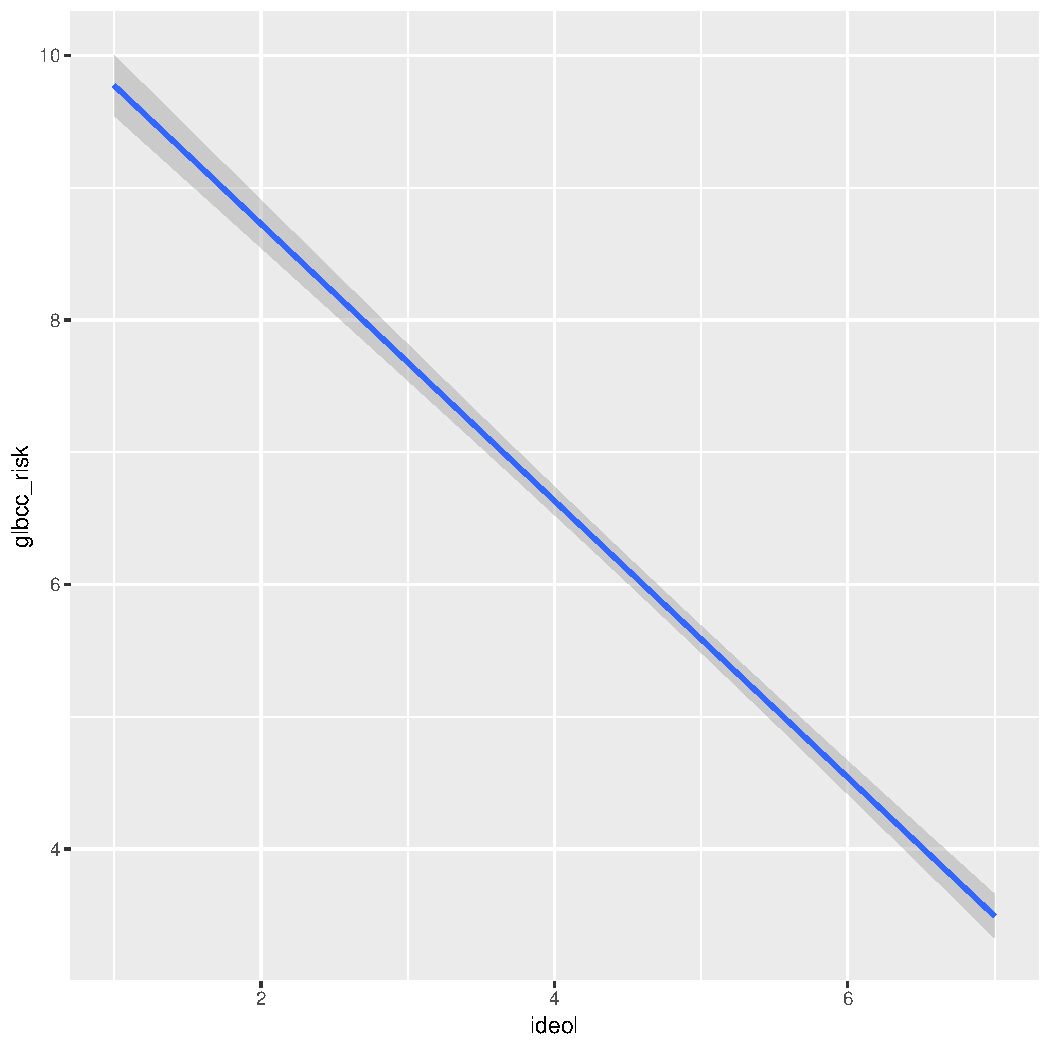
\includegraphics[width=3.5in, height=3.5in]{09_InterpretSimple/effectsplot.pdf}%filename
\caption{Bivariate Regression Plot\label{fig:effectsplot}}
\end{figure} 

\noindent \textbf{Cleaning up the R Environment}

If you recall, at the beginning of the chapter, we created several temporary data sets.  We should take the time to clear up our workspace for the next chapter.
\begin{knitrout}
\definecolor{shadecolor}{rgb}{0.969, 0.969, 0.969}\color{fgcolor}\begin{kframe}
\begin{alltt}
\hlcom{# we can clean up from the temporary data sets for this}
\hlcom{# chapter.}
\hlkwd{rm}\hlstd{(ds.omit)}  \hlcom{#remove the omit data set}
\end{alltt}
\end{kframe}
\end{knitrout}

\section{Summary} 

This chapter has focused on two key aspects of simple regression models -- hypothesis testing and  measures of the goodness of model fit. With respect to the former, we focused on the residual standard error, and its role in determining the probability that our model estimates, $B$ and $A$, are just random departures from a population in which $\beta$ and $\alpha$ are zero. We showed, using \texttt{R}, how to calculate the residual standard errors for $A$ and $B$ and, using them, to calculate the t-statistics and associated probabilities for hypothesis testing. For model fit, we focused on model covariation and correlation, and finished up with a discussion of the coefficient of determination -- $R^{2}$. So now you are in a position to use simple regression, and to wage unremitting geek-war on those whose models are endowed with lesser $R^{2}s$.





\chapter{OLS Assumptions and Simple Regression Diagnostics}

Now that you know how to run and interpret simple regression results, we return to the matter of the underlying assumptions of OLS models, and the steps we can take to determine whether those assumptions have been violated. We begin with a quick review of the conceptual use of residuals, then turn to a set of ``visual diagnostics" that can help you identify possible problems in your model. We conclude with a set of steps you can take to address model problems, should they be encountered. As with the previous chapter, we will use examples drawn from the \texttt{tbur} data.  As always, we recommend that you try the analyses in the chapter as you read.

\section{A Recap of Modeling Assumptions}

Recall from Chapter 4 that we identified three key assumptions about the error term that are necessary for OLS to provide unbiased, efficient linear estimators; a) errors have identical distributions, b) errors are independent, c) errors are normally distributed.\footnote{Again, we assume only that the \textbf{means} of the errors drawn from repeated samples of observations will be normally distributed -- but we will often find that errors in a particular sample deviate significantly from a normal distribution.}

\begin{grbox}
\greybox{\textbf{Error Assumptions}
  \begin{enumerate}  
\item Errors have identical distributions
  \begin{center}
    $E(\epsilon^{2}_{i}) = \sigma^2_{\epsilon}$
  \end{center}
\item Errors are independent of $X$ and other $\epsilon_{i}$
  \begin{center}
    $E(\epsilon_{i}) \equiv E(\epsilon|x_{i}) = 0$ 
    
    and 
    
    $E(\epsilon_{i}) \neq E(\epsilon_{j})$ for $i \neq j$
  \end{center}
\item Errors are normally distributed
  \begin{center}
    $\epsilon_{i} \sim N(0,\sigma^2_{\epsilon})$
  \end{center}
\end{enumerate}}
\end{grbox}

Taken together these assumption mean that the error term has a normal, independent, and identical distribution (normal i.i.d.). Figure \ref{fig:residdist} shows what these assumptions would imply for the distribution of residuals around the predicted values of $Y$ given $X$.


\begin{figure}
  \centering
  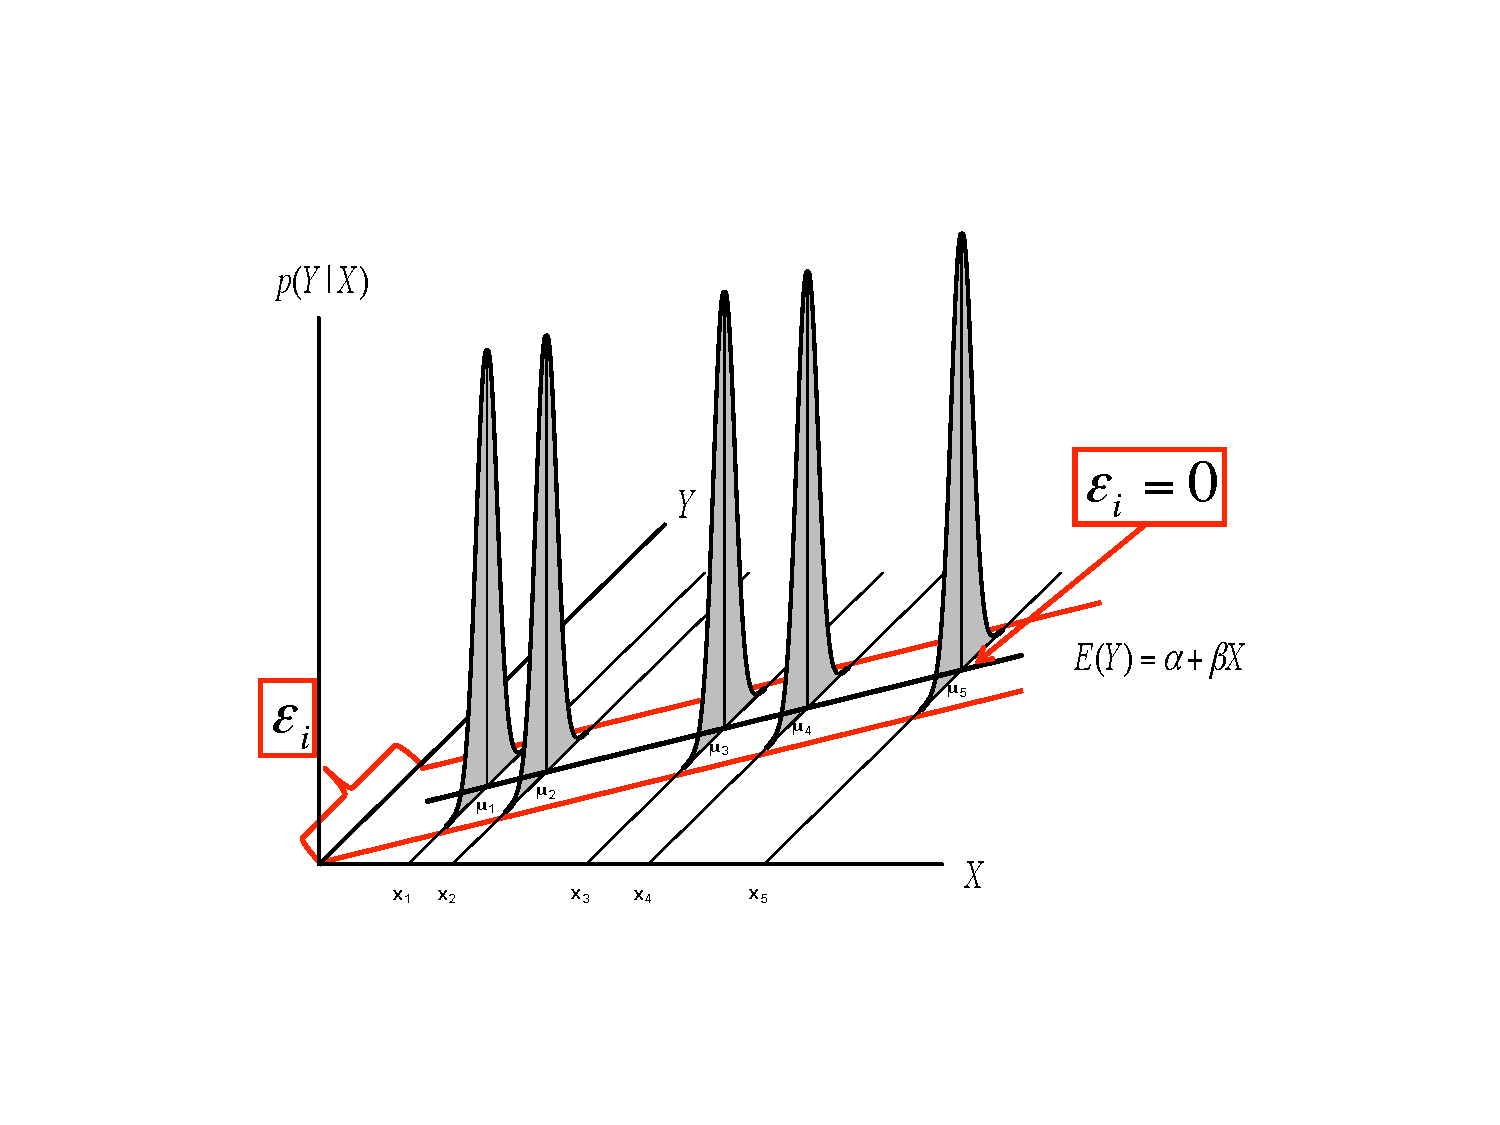
\includegraphics[width=4in]{10_SimpleDiagnostics/residdist.pdf}%filename
  \caption{Assumed Distributions of OLS Residuals \label{fig:residdist}}
\end{figure}

How can we determine whether our residuals approximate the expected pattern? The most straight-forward approach is to visually examine the distribution of the residuals over the range of the predicted values for $Y$. If all is well, there should be no obvious pattern to the residuals -- they should appear as a ``sneeze plot" (i.e.,  it looks like you sneezed on the plot. How gross!) as shown in Figure \ref{fig:sneeze}.

\begin{figure}
  \centering
  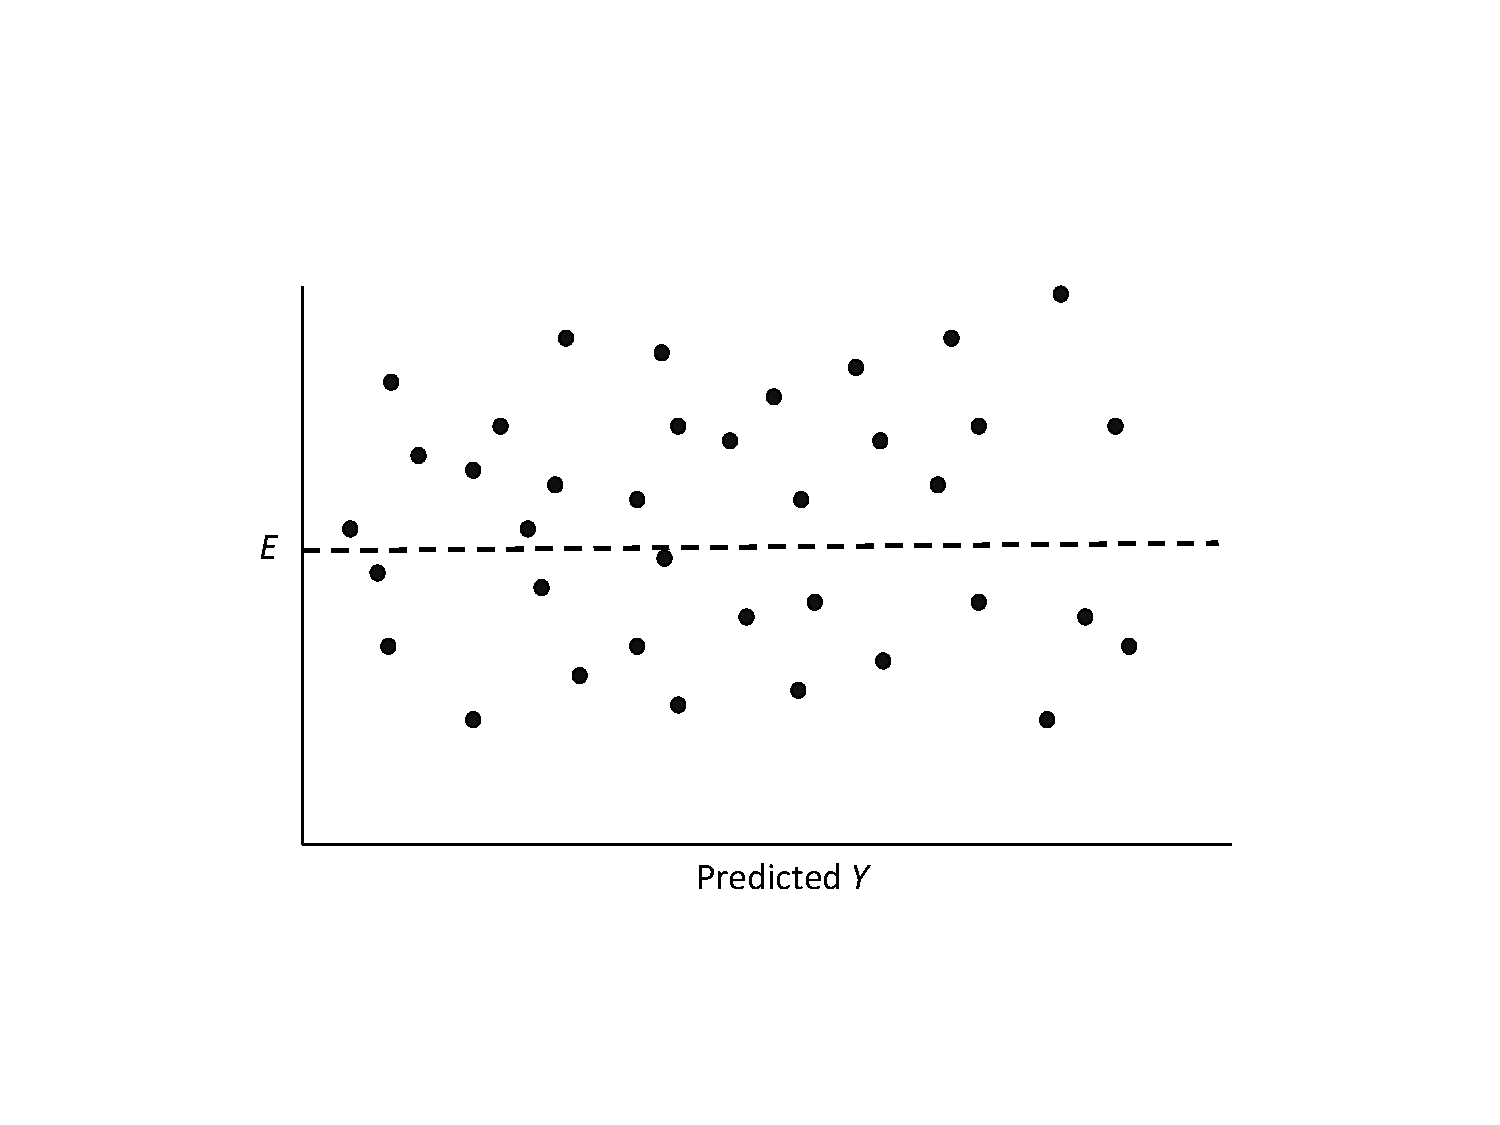
\includegraphics[width=4in]{10_SimpleDiagnostics/sneeze.pdf}%filename
  \caption{Ideal Pattern of Residuals from a Simple OLS Model \label{fig:sneeze}}
\end{figure}

Generally, there is no pattern in such a sneeze plot of residuals. One of the difficulties we have, as human beings, is that we tend to look at randomness and \texttt{perceive} patterns. Our brains are wired to see patterns, even where their are none. Moreover, with random distributions there will in some samples be clumps and gaps that do \texttt{appear} to depict some kind of order when in fact there is none. There is the danger, then, of over-interpreting the pattern of residuals to see problems that aren't there. The key is to know what kinds of patterns to look for, so when you do observe one you will know it.

\section{When Things Go Bad with Residuals} 

Residual analysis is the process of looking for \texttt{signature patterns} in the residuals that are indicative of failure in the underlying assumptions of OLS regression. Different kinds of problems lead to different patterns in the residuals.

\subsection{``Outlier" Data}

Sometimes our data include unusual cases that behave differently from most of our observations. This may happen for a number of reasons. The most typical is that the data have been mis-coded, with some subgroup of the data having numerical values that lead to large residuals. Cases like this can also arise when a subgroup of the cases differ from the others in how $X$ influences $Y$, and that difference has not been captured in the model. This is a problem referred to as the omission of important independent variables.\footnote{Political scientists who study US electoral politics have had to account for unusual observations in the Southern states. Failure in the model to account for these differences would lead to prediction error and ugly patterns in the residuals. Sadly, Professor Gaddie notes that scholars have not been sufficiently careful -- or perhaps well-trained? -- to do this right. Professor Gaddie notes:  ``... instead of working to achieve better model specification through the application of theory and careful thought, in the 1960s and 1970s electoral scholars instead just threw out the South and all senate races, creating the perception that the United States had 39 states and a unicameral legislature."} Figure \ref{fig:unusual_dat} shows a stylized example, with a cluster of residuals falling at considerable distance from the rest. 

\begin{figure}
  \centering
  \includegraphics[width=4in]%
    {10_SimpleDiagnostics/unusual_dat.pdf}% picture filename
  \caption{Unusual Data Patterns in Residuals \label{fig:unusual_dat}}
\end{figure}

This is a case of influential outliers. The effect of such outliers can be significant, as the OLS estimates of $A$ and $B$ seek to minimize overall squared error. In the case of Figure \ref{fig:unusual_dat}, the effect would be to shift the estimate of $B$ to accommodate the unusual observations, as illustrated in Figure \ref{fig:unusual_dat2}. One possible response would be to omit the unusual observations, as shown in Figure \ref{fig:unusual_dat2}. Another would be to consider, theoretically and empirically, why these observations are unusual. Are they, perhaps, miscoded? Or are they codes representing missing values (e.g., ``-99")?

If they are not mis-codes, perhaps these outlier observations manifest a different kind of relationship between $X$ and $Y$, which might in turn require a revised theory and model. We will address some modeling options to address this possibility when we explore multiple regression, in Part III of this book.

\begin{figure}
  \centering
  \includegraphics[width=4in]%
    {10_SimpleDiagnostics/unusual_dat2.pdf}% picture filename
  \caption{Implications of Unusual Data Patterns in Residuals \label{fig:unusual_dat2}}
\end{figure}

In sum, outlier analysis looks at residuals for patterns in which some observations deviate widely from others. If that deviation is influential, changing estimates of $A$ and $B$ as shown in Figure \ref{fig:unusual_dat2}, then you must examine the observations to determine whether they are mis-coded. If not, you can evaluate whether the cases are theoretically distinct, such that the influence of $X$ on $Y$ is likely to be different than for other cases. If you conclude that this is so, you will need to respecify your model to account for these differences. We will discuss some options for doing that later in this chapter, and again in our discussion of multiple regression.

\subsection{Non-Constant Variance}

A second thing to look for in visual diagnostics of residuals is non-constant variance, or
\texttt{heteroscedasticity}. In this case, the variation in the residuals over the range of predicted values for $Y$ should be roughly even. A problem occurs when that variation changes substantially as the predicted value of $Y$ changes, as is illustrated in Figure \ref{fig:hetero10}.

\begin{figure}
  \centering
  \includegraphics[width=4in]%
    {10_SimpleDiagnostics/hetero.pdf}% picture filename
  \caption{Non-Constant Variance in the Residuals \label{fig:hetero10}}
\end{figure}

As Figure \ref{fig:hetero10} shows, the width of the spread of the residuals grows as the predicted value of $Y$ increases, making a fan-shaped pattern. Equally concerning would be a case of a ``reverse fan", or a pattern with a bulge in the middle and very ``tight" distributions of residuals at either extreme. These would all be cases in which the assumption of constant-variance in the residuals (or ``homoscedasticity") fails, and are referred to as instances of heteroscedasticity.

What are the implications of heteroscedasticity? Our hypothesis tests for the estimated coefficients ($A$ and $B$) are based on the assumption that the standard errors of the estimates (see the prior chapter) are normally distributed. If inspection of your residuals provides evidence to question that assumption, then the interpretation of the t-values and p-values may be problematic. Intuitively, in such a case the precision of our estimates of $A$ and $B$ are not constant -- but rather will depend on the predicted value of $Y$. So you might be estimating $B$ relatively precisely in some ranges of $Y$, and less precisely in others. That means you cannot depend on the estimated t and p-values to test your hypotheses.

\subsection{Non-Linearity in the Parameters}

One of the primary assumptions of simple OLS regression is that the estimated slope parameter (the $B$) will be constant, and therefore the model will be linear. Put differently, the effect of any change in $X$ on $Y$  should be constant over the range of $Y$. Thus, if our assumption is correct, the pattern of the residuals should be roughly symmetric, above and below zero, over the range of predicted values.

If the real relationship between $X$ and $Y$ is not linear, however, the predicted (linear) values for $Y$ will systematically depart from the (curved) relationship that is represented in the data. Figure \ref{fig:simplenonlin} shows the kind of pattern we would expect in our residuals if the observed relationship between $X$ and $Y$ is a strong curve, when we attempt to model it as if it were linear.

\begin{figure}
  \centering
  \includegraphics[width=4in]%
    {10_SimpleDiagnostics/simplenonlin.pdf}% picture filename
  \caption{Non-Linearity in the Residuals \label{fig:simplenonlin}}
\end{figure}

What are the implications of non-linearity? First, because the slope is non-constant, the estimate of $B$ will be biased. In the illustration shown in Figure \ref{fig:simplenonlin}, $B$ would underestimate the value of $Y$ in both the low and high ranges of the predicted value of $Y$, and overestimate it in the mid-range. In addition, the standard errors of the residuals will be large, due to systematic over- and under-estimation of $Y$, making the model very inefficient (or imprecise). 

\section{Application of Residual Diagnostics}

This far we have used rather simple illustrations of residual diagnostics and the kinds of patterns to look for. But you should be warned that, in real applications, the patterns are rarely so clear. So we will walk through an example diagnostic session, using the the \texttt{tbur} data set.

Our in-class lab example focuses on the relationship between political ideology (``ideology" in our dataset) as a predictor of the perceived risks posed by climate change (``gccrsk"). The model is specified in \texttt{R} as follows:

\begin{knitrout}
\definecolor{shadecolor}{rgb}{0.969, 0.969, 0.969}\color{fgcolor}\begin{kframe}
\begin{alltt}
\hlstd{OLS_env} \hlkwb{<-} \hlkwd{lm}\hlstd{(ds}\hlopt{$}\hlstd{glbcc_risk} \hlopt{~} \hlstd{ds}\hlopt{$}\hlstd{ideol)}
\end{alltt}
\end{kframe}
\end{knitrout}

\noindent Using the summary command in $R$, we can review the results.
\begin{knitrout}
\definecolor{shadecolor}{rgb}{0.969, 0.969, 0.969}\color{fgcolor}\begin{kframe}
\begin{alltt}
\hlkwd{summary}\hlstd{(OLS_env)}
\end{alltt}
\begin{verbatim}
## 
## Call:
## lm(formula = ds$glbcc_risk ~ ds$ideol)
## 
## Residuals:
##    Min     1Q Median     3Q    Max 
## -8.726 -1.633  0.274  1.459  6.506 
## 
## Coefficients:
##             Estimate Std. Error t value            Pr(>|t|)    
## (Intercept) 10.81866    0.14189   76.25 <0.0000000000000002 ***
## ds$ideol    -1.04635    0.02856  -36.63 <0.0000000000000002 ***
## ---
## Signif. codes:  0 '***' 0.001 '**' 0.01 '*' 0.05 '.' 0.1 ' ' 1
## 
## Residual standard error: 2.479 on 2511 degrees of freedom
##   (34 observations deleted due to missingness)
## Multiple R-squared:  0.3483,	Adjusted R-squared:  0.348 
## F-statistic:  1342 on 1 and 2511 DF,  p-value: < 0.00000000000000022
\end{verbatim}
\end{kframe}
\end{knitrout}

Note that, as was discussed in the prior chapter, the estimated value for $B$ is negative and highly statistically significant. This indicates that the more conservative the survey respondent, the lower the perceived risks attributed to climate change. Now we will use these model results and the associated residuals to evaluate the key assumptions of OLS, beginning with linearity. 

\subsection{Testing for Non-Linearity}
One way to test for non-linearity is to fit the model to a polynomial functional form. This sounds impressive, but is quite easy to do and understand (really!). All you need to do is include the square of the independent variable as a second predictor in the model.  A significant regression coefficient on the squared variable indicates problems with linearity. To do this, we first produce the squared variable.

\begin{knitrout}
\definecolor{shadecolor}{rgb}{0.969, 0.969, 0.969}\color{fgcolor}\begin{kframe}
\begin{alltt}
\hlcom{# first we square the ideology variable and create a new}
\hlcom{# variable to use in our model.}
\hlstd{ds}\hlopt{$}\hlstd{ideology2} \hlkwb{<-} \hlstd{ds}\hlopt{$}\hlstd{ideol}\hlopt{^}\hlnum{2}
\hlkwd{summary}\hlstd{(ds}\hlopt{$}\hlstd{ideology2)}
\end{alltt}
\begin{verbatim}
##    Min. 1st Qu.  Median    Mean 3rd Qu.    Max.    NA's 
##    1.00   16.00   25.00   24.65   36.00   49.00      23
\end{verbatim}
\end{kframe}
\end{knitrout}

\noindent Next, we run the regression with the original independent variable and our new squared variable.  Finally, we check the regression output.

\begin{knitrout}
\definecolor{shadecolor}{rgb}{0.969, 0.969, 0.969}\color{fgcolor}\begin{kframe}
\begin{alltt}
\hlstd{OLS_env2} \hlkwb{<-} \hlkwd{lm}\hlstd{(glbcc_risk} \hlopt{~} \hlstd{ideol} \hlopt{+} \hlstd{ideology2,} \hlkwc{data} \hlstd{= ds)}
\hlkwd{summary}\hlstd{(OLS_env2)}
\end{alltt}
\begin{verbatim}
## 
## Call:
## lm(formula = glbcc_risk ~ ideol + ideology2, data = ds)
## 
## Residuals:
##    Min     1Q Median     3Q    Max 
## -8.564 -1.808  0.192  1.448  6.863 
## 
## Coefficients:
##             Estimate Std. Error t value             Pr(>|t|)    
## (Intercept)  9.58238    0.28397  33.745 < 0.0000000000000002 ***
## ideol       -0.34444    0.14274  -2.413               0.0159 *  
## ideology2   -0.08234    0.01641  -5.018          0.000000558 ***
## ---
## Signif. codes:  0 '***' 0.001 '**' 0.01 '*' 0.05 '.' 0.1 ' ' 1
## 
## Residual standard error: 2.467 on 2510 degrees of freedom
##   (34 observations deleted due to missingness)
## Multiple R-squared:  0.3548,	Adjusted R-squared:  0.3543 
## F-statistic: 690.1 on 2 and 2510 DF,  p-value: < 0.00000000000000022
\end{verbatim}
\end{kframe}
\end{knitrout}
A significant coefficient on the squared ideology variable informs us that we probably have a non-linearity problem. The significant and negative coefficient for the square of ideology means that the curve steepens (perceived risks fall faster) as the scale shifts further up on the conservative side of the scale. We can supplement the polynomial regression test by producing a residual plot with a formal Tukey test. The residual plot (\texttt{car} package \texttt{residualPlots} function) displays the Pearson fitted values against the model's observed values. Ideally, the plots will produce flat red lines; curved lines represent non-linearity.  The output for the Tukey test is visible in the $R$ workspace.  The null hypothesis for the Tukey test is a linear relationship, so a significant p-value is indicative of non-linearity.  The tukey test is reported as part of the \texttt{residualPlots} function in the \texttt{car} package.

\begin{knitrout}
\definecolor{shadecolor}{rgb}{0.969, 0.969, 0.969}\color{fgcolor}\begin{kframe}
\begin{alltt}
\hlcom{# A significant p-value indicates non-linearity using the}
\hlcom{# Tukey test}
\end{alltt}
\begin{verbatim}
##            Test stat Pr(>|Test stat|)    
## ds$ideol     -5.0181     0.0000005584 ***
## Tukey test   -5.0181     0.0000005219 ***
## ---
## Signif. codes:  0 '***' 0.001 '**' 0.01 '*' 0.05 '.' 0.1 ' ' 1
## pdf 
##   2
\end{verbatim}
\end{kframe}
\end{knitrout}

\begin{figure}
  \centering
  \includegraphics[width=4in]%
    {10_SimpleDiagnostics/nonlinideology.pdf}% picture filename
  \caption{Residual Plots Examining Model Linearity \label{fig:nonlinideology}}
\end{figure}

The curved red lines in Figure \ref{fig:nonlinideology} in the residual plots and significant Tukey test indicate a non-linear relationship in the model.  This is a serious violation of a core assumption of OLS regression, which means that the estimate of $B$ is likely to be biased. Our findings suggest that the relationship between ideology and perceived risks of climate change is approximately linear from ``strong liberals" to those who are ``leaning Republican". But perceived risks seem to drop off more rapidly as the scale rises toward ``strong Republican."

\subsection{Testing for Normality in Model Residuals}
Testing for normality in the model residuals will involve using many of the techniques demonstrated in previous chapters.  The first step is to  graphically display the residuals in order to see how closely the model residuals resemble a normal distribution.  A formal test for normality is also included in the demonstration.

Start by creating a histogram of the model residuals.

\begin{knitrout}
\definecolor{shadecolor}{rgb}{0.969, 0.969, 0.969}\color{fgcolor}\begin{kframe}
\begin{alltt}
\hlstd{OLS_env}\hlopt{$}\hlstd{residuals} \hlopt \hlcom{# Pipe the residuals to a data frame}
  \hlkwd{data.frame}\hlstd{()} \hlopt \hlcom{# Pipe the data frame to ggplot}
  \hlkwd{ggplot}\hlstd{(}\hlkwd{aes}\hlstd{(OLS_env}\hlopt{$}\hlstd{residuals))} \hlopt{+}
  \hlkwd{geom_histogram}\hlstd{(}\hlkwc{bins} \hlstd{=} \hlnum{16}\hlstd{)}
\end{alltt}
\end{kframe}
\end{knitrout}

\begin{figure}
  \centering
  \includegraphics[width=4in]%
    {10_SimpleDiagnostics/histideology.pdf}% picture filename
  \caption{Histogram of Model Residuals \label{fig:histideology}}
\end{figure}

The histogram in figure \ref{fig:histideology} indicates that the residuals are approximately normally distributed, but there appears to be a negative skew.  Next, we can create a smoothed density of the model residuals compared to a theoretical normal distribution.

\begin{knitrout}
\definecolor{shadecolor}{rgb}{0.969, 0.969, 0.969}\color{fgcolor}\begin{kframe}
\begin{alltt}
\hlstd{OLS_env}\hlopt{$}\hlstd{residuals} \hlopt \hlcom{# Pipe the residuals to a data frame}
  \hlkwd{data.frame}\hlstd{()} \hlopt \hlcom{# Pipe the data frame to ggplot}
  \hlkwd{ggplot}\hlstd{(}\hlkwd{aes}\hlstd{(OLS_env}\hlopt{$}\hlstd{residuals))} \hlopt{+}
  \hlkwd{geom_density}\hlstd{(}\hlkwc{adjust} \hlstd{=} \hlnum{2}\hlstd{)} \hlopt{+}
  \hlkwd{stat_function}\hlstd{(}\hlkwc{fun} \hlstd{= dnorm,} \hlkwc{args} \hlstd{=} \hlkwd{list}\hlstd{(}\hlkwc{mean} \hlstd{=} \hlkwd{mean}\hlstd{(OLS_env}\hlopt{$}\hlstd{residuals),}
                                         \hlkwc{sd} \hlstd{=} \hlkwd{sd}\hlstd{(OLS_env}\hlopt{$}\hlstd{residuals)),}
                \hlkwc{color} \hlstd{=} \hlstr{"red"}\hlstd{)}
\hlkwd{dev.off}\hlstd{()}
\end{alltt}
\end{kframe}
\end{knitrout}

\begin{figure}
  \centering
  \includegraphics[width=4in]%
    {10_SimpleDiagnostics/densityideology.pdf}% picture filename
  \caption{Smoothed Density Plot of Model Residuals \label{fig:densityideology}}
\end{figure}
\FloatBarrier

Figure \ref{fig:densityideology} indicates the model residuals deviate slightly from a normal distributed because of a slightly negative skew and a mean higher than we would expect in a normal distribution.  Our final ocular examination of the residuals will be a quartile plot %(using the \texttt{stat_qq} function from the \texttt{ggplot2} package).

\begin{knitrout}
\definecolor{shadecolor}{rgb}{0.969, 0.969, 0.969}\color{fgcolor}\begin{kframe}
\begin{alltt}
\hlstd{OLS_env}\hlopt{$}\hlstd{residuals} \hlopt \hlcom{# Pipe the residuals to a data frame}
  \hlkwd{data.frame}\hlstd{()} \hlopt \hlcom{# Pipe the data frame to ggplot}
  \hlkwd{ggplot}\hlstd{(}\hlkwd{aes}\hlstd{(}\hlkwc{sample} \hlstd{= OLS_env}\hlopt{$}\hlstd{residuals))} \hlopt{+}
  \hlkwd{stat_qq}\hlstd{()} \hlopt{+}
  \hlkwd{stat_qq_line}\hlstd{()}
\end{alltt}
\end{kframe}
\end{knitrout}


\begin{figure}
  \centering
  \includegraphics[width=4in]%
    {10_SimpleDiagnostics/QQideology.pdf}% picture filename
  \caption{Quartile Plot of Model Residuals \label{fig:QQideology}}
\end{figure}
\FloatBarrier

According to Figure \ref{fig:QQideology}, it appears as if the residuals are normally distributed except for the tails of the distribution.   Taken together the graphical representations of the residuals suggest modest non-normality.  As a final step, we can conduct a formal Shapiro-Wilk test for normality.  The null hypothesis for a Shapiro-Wilk test is a normal distribution, so we do not want to see a significant p-value.

\begin{knitrout}
\definecolor{shadecolor}{rgb}{0.969, 0.969, 0.969}\color{fgcolor}\begin{kframe}
\begin{alltt}
\hlcom{# a significant value p-value potentially indicates the data}
\hlcom{# is not normally distributed.}
\hlkwd{shapiro.test}\hlstd{(OLS_env}\hlopt{$}\hlstd{residuals)}
\end{alltt}
\begin{verbatim}
## 
## 	Shapiro-Wilk normality test
## 
## data:  OLS_env$residuals
## W = 0.98901, p-value = 0.000000000000551
\end{verbatim}
\end{kframe}
\end{knitrout}

The Shapiro-Wilk test confirms what we observed in the graphical displays of the model residuals -- the residuals are not normally distributed.   Recall that our dependent variable (gccrsk) appears to have a non-normal distribution. This could be the root of the non-normality found in  the model residuals. Given this information, steps must be taken to assure that the model residuals meet the required OLS assumptions. One possibility would be to transform the dependent variable (glbccrisk) in order to induce a normal distribution. Another might be to add a polynomial term to the independent variable (ideology) as was done above. In either case, you would need to recheck the residuals in order to see if the model revisions adequately dealt with the problem. We suggest that you do just that!

\subsection{Testing for Non-Constant Variance in the Residuals}

Testing for non-constant variance (heteroscedasticity) in a model is fairly straightforward. We can start by creating a spread-level plot  that fits the studentized residuals against the model's fitted values.  A line with a non-zero slope is indicative of heteroscedasticity. Figure \ref{fig:spreadlvlideology} displays the spread-level plot from the \texttt{car} package.

\begin{knitrout}
\definecolor{shadecolor}{rgb}{0.969, 0.969, 0.969}\color{fgcolor}\begin{kframe}
\begin{alltt}
\hlkwd{spreadLevelPlot}\hlstd{(OLS_env)}
\end{alltt}
\end{kframe}
\end{knitrout}

\begin{figure}
  \centering
  \includegraphics[width=4in]%
    {10_SimpleDiagnostics/spreadlvlideology.pdf}% picture filename
  \caption{Spread-Level Plot of Model Residuals \label{fig:spreadlvlideology}}
\end{figure}
\FloatBarrier

The negative slope on the red line in Figure \ref{fig:spreadlvlideology} indicates the model may contain heteroscedasticity.  We can also perform  a formal test for non constant variance.  The null hypothesis is constant variance, so we do not want to see a significant p-value.

\begin{knitrout}
\definecolor{shadecolor}{rgb}{0.969, 0.969, 0.969}\color{fgcolor}\begin{kframe}
\begin{alltt}
\hlcom{# a significant value indicates potential heteroscedasticity}
\hlcom{# issues.}
\hlkwd{ncvTest}\hlstd{(OLS_env)}
\end{alltt}
\begin{verbatim}
## Non-constant Variance Score Test 
## Variance formula: ~ fitted.values 
## Chisquare = 68.107, Df = 1, p = < 0.000000000000000222
\end{verbatim}
\end{kframe}
\end{knitrout}

The significant p-value on the non-constant variance test informs us that there is a problem with heteroscedasticity in the model.  This is yet another violation of the core assumptions of OLS regression, and it brings into doubt our hypothesis tests.

\subsection{Examining Outlier Data}

There are a number of ways to examine outlying observations in an OLS regression. This section briefly illustrates a a subset of analytical tests that will provide a useful assessment of potentially important outliers.  The purpose of examining outlier data is twofold.  First, we want to make sure there are not any mis-coded or invalid data influencing our regression. For example, an outlying observation with a value of ``-99" would very likely bias our results, and obviously needs to be  corrected. Second, outlier data may indicate the need to theoretically reconceptualize our model.  Perhaps the relationship in the model is mis-specified, with outliers at the extremes of a variable suggesting a non-linear relationship. Or it may be that a  subset of cases respond differently to the independent variable, and therefore must be treated as ``special cases" in the model. Examining outliers allows us to identify and address these potential problems.

One of the first things we can do is perform a Bonferroni Outlier Test. The Bonferroni Outlier Tests uses a $t$ distribution to test whether the model's largest studentized residual value's outlier status is statistically different from the other observations in the model.  A significant p-value indicates an extreme outlier that warrants further examination.  We use the \texttt{outlierTest} function in the \texttt{car} package to perform a Bonferroni Outlier Test.

\begin{knitrout}
\definecolor{shadecolor}{rgb}{0.969, 0.969, 0.969}\color{fgcolor}\begin{kframe}
\begin{alltt}
\hlcom{# a significant p-value indicates extreme case for review}
\hlkwd{outlierTest}\hlstd{(OLS_env)}
\end{alltt}
\begin{verbatim}
## No Studentized residuals with Bonferonni p < 0.05
## Largest |rstudent|:
##      rstudent unadjusted p-value Bonferonni p
## 589 -3.530306         0.00042255           NA
\end{verbatim}
\end{kframe}
\end{knitrout}

According to the R output, the Bonferroni p-value for the largest (absolute) residual is not statistically significant.  While this test is important for identifying a potentially significant outlying  observation, it is not a panacea for checking for patterns in outlying data.  Next we will examine the model's df.betas in order to see which observations exert the most influence on the model's regression coefficients. $Dfbetas$ are measures of how much the regression coefficient changes when observation $i$ is omitted.  Larger values indicate an observation that has considerable influence on the model.   

A useful method for finding dfbeta obervations is to use the \texttt{dfbetaPlots} function in the \texttt{car} package.  We specify the option \texttt{id.n=2} to show the two largest df.betas.  See figure \ref{fig:dfbetaPlots}.

\begin{knitrout}
\definecolor{shadecolor}{rgb}{0.969, 0.969, 0.969}\color{fgcolor}\begin{kframe}
\begin{alltt}
\hlstd{plotdb} \hlkwb{<-} \hlkwd{dfbetaPlots}\hlstd{(OLS_env,} \hlkwc{id.n} \hlstd{=} \hlnum{3}\hlstd{)}
\end{alltt}
\end{kframe}
\end{knitrout}

\begin{figure}
  \centering
  \includegraphics[width=4in]%
    {10_SimpleDiagnostics/dfbetaPlots.pdf}% picture filename
  \caption{Plot of Model dfbetas Values using \texttt{dfbetaPlots} function \label{fig:dfbetaPlots}}
\end{figure}
\FloatBarrier

\begin{knitrout}
\definecolor{shadecolor}{rgb}{0.969, 0.969, 0.969}\color{fgcolor}\begin{kframe}
\begin{alltt}
\hlcom{# Check the observations with high dfbetas.  We see the}
\hlcom{# values 589 and 615 returned.  We only want to see results}
\hlcom{# from columns gccrsk and ideology in tbur.data.}
\hlstd{ds[}\hlkwd{c}\hlstd{(}\hlnum{589}\hlstd{,} \hlnum{615}\hlstd{),} \hlkwd{c}\hlstd{(}\hlstr{"glbcc_risk"}\hlstd{,} \hlstr{"ideol"}\hlstd{)]}
\end{alltt}
\begin{verbatim}
##     glbcc_risk ideol
## 589          0     2
## 615          0     2
\end{verbatim}
\end{kframe}
\end{knitrout}

These observations are interesting because they identify a potential problem in our model specification.  Both observations are considered outliers because the respondents self-identified as ``liberal" (ideology = 1) and rated their perceived  risk of global climate change as 0.  These values deviate substantially from the norm for other strong liberals in the dataset.  Remember, as we saw earlier, our model has a problem with non-linearity -- these outlying observations seem to corroborate this finding.  Examination of outliers sheds some light on the issue.

Finally, we can produce a plot that combines studentized residuals, ``hat values", and Cook's D distances (these are measures of the amount of influence observations have on the model) using circles as an indicator of influence -- the larger the circle, the greater the influence.  Figure \ref{fig:bubbleideology2} displays the combined influence plot.  In addition, the \texttt{influencePlot} function returns the values of greatest influence.

\begin{knitrout}
\definecolor{shadecolor}{rgb}{0.969, 0.969, 0.969}\color{fgcolor}\begin{kframe}
\begin{alltt}
\hlkwd{influencePlot}\hlstd{(OLS_env)}
\end{alltt}
\begin{verbatim}
##         StudRes         Hat          CookD
## 20   0.09192603 0.002172497 0.000009202846
## 30   0.09192603 0.002172497 0.000009202846
## 589 -3.53030574 0.001334528 0.008289418537
## 615 -3.53030574 0.001334528 0.008289418537
## pdf 
##   2
\end{verbatim}
\end{kframe}
\end{knitrout}

\begin{figure}
  \centering
  \includegraphics[width=4in]%
    {10_SimpleDiagnostics/bubbleideology.pdf}% picture filename
  \caption{Influence Bubble Plot \label{fig:bubbleideology2}}
\end{figure}
\FloatBarrier

\noindent Figure \ref{fig:bubbleideology2} indicates that there are a number of cases that warrant further examination.  We are already familiar with 589 and 615  Let's add 20, 30, 90 and 1052.

\begin{knitrout}
\definecolor{shadecolor}{rgb}{0.969, 0.969, 0.969}\color{fgcolor}\begin{kframe}
\begin{alltt}
\hlcom{# review the results}
\hlstd{ds[}\hlkwd{c}\hlstd{(}\hlnum{589}\hlstd{,} \hlnum{615}\hlstd{,} \hlnum{20}\hlstd{,} \hlnum{30}\hlstd{,} \hlnum{90}\hlstd{,} \hlnum{1052}\hlstd{),} \hlkwd{c}\hlstd{(}\hlstr{"glbcc_risk"}\hlstd{,} \hlstr{"ideol"}\hlstd{)]}
\end{alltt}
\begin{verbatim}
##      glbcc_risk ideol
## 589           0     2
## 615           0     2
## 20           10     1
## 30           10     1
## 90           10     1
## 1052          3     6
\end{verbatim}
\end{kframe}
\end{knitrout}

One important take-away from a visual examination of these observations is that there do not appear to be any completely mis-coded or invalid data affecting our model. In general, even the most influential observations do not appear to be implausible cases.  Observations 589 and 615 \footnote{Of note, observations 20, 30, and 90 and 1052 are returned as well.  There doesn't appear to be anything special about these four observations.  Part of this may be due to the bivariate relationship and how the \texttt{influcencePlot} function weights the data.  The results are included for your review.} present an interesting problem regarding  theoretical and model specification. These observations represent respondents who self-reported as  ``liberal" (ideology=2) and also rated the perceived risk of global climate change as 0 out of 10. These observations therefore deviate from the model's expected values (``strong liberal" respondents, on average, believed global climate change represents a high risk).  Earlier in our diagnostic testing we found a problem with non-linearity. Taken together, it looks like the non-linearity in our model is due to observations at the ideological extremes.  One way we can deal with this problem is to include a squared ideology variable (a polynomial) in the model, as illustrated earlier in this chapter. However, it is also important to note this non-linear relationship in the theoretical conceptualization of our model. Perhaps there is something special about people with extreme ideologies that needs to be taken into account when attempting to predict perceived risk of global climate change. This finding should also inform our examination of post-estimation predictions -- something that will be covered later in this text.

\section{So Now What? Implications of Residual Analysis}

What should you do if you observe patterns in the residuals that seem to violate the assumptions of OLS? If you find deviant cases -- outliers that are shown to be highly influential -- you need to first evaluate the specific cases (observations). Is it possible that the data were miscoded? We hear of many instances in which missing value codes (often ``-99") were inadvertently left in the dataset. \texttt{R} would treat such values as if they were real data, often generating glaring and influential outliers. Should that be the case, recode the offending variable observation as missing (``NA") and try again.  

%for future reference - http://connectmv.com/tutorials/r-tutorial/investigating-outliers-discrepancies-and-other-influential-points/
% we can use a process to quickly remove the results.

But what if there is no obvious coding problem? It may be that the influential outlier is appropriately measured, but that the observation is different in some theoretically important way. Suppose, for example, that your model included some respondents who -- rather than diligently answering your questions -- just responded at random to your survey questions. They would introduce noise and error. If you could measure these slackers, you could either exclude them or include a control variable in your model to account for their different patterns of responses. We will discuss inclusion of model controls when we turn to multiple regression modeling in later chapters.

What if your residual analysis indicates the presence of heteroscedasticity? Recall that this will undermine your ability to do hypothesis tests in OLS. There are several options. If the variation in fit over the range of the predicted value of $Y$ could plausibly result from the omission of an important explanatory variable, you should respecify your model accordingly (more on this later in this book). It is often the case that you can improve the distribution of residuals by including important but previously omitted variables. Measures of income, when left out of consumer behavior models, often have this effect.

Another approach is to use a different modeling approach that accounts for the heteroscedasticity in the estimated standard error. Of particular utility are robust estimators, which can be employed using the \texttt{rlm} (robust linear model) function in the \texttt{MASS} package. This approach increases the magnitude of the estimated standard errors, reducing the t-values and resulting p-values. That means that the ``cost" of running robust estimators is that the precision of the estimates is reduced.

Evidence of non-linearity in the residuals presents a thorny problem. This is a basic violation of a central assumption of OLS, resulting in biased estimates of $A$ and $B$. What can you do? First, you can respecify your model to include a polynomial; you would include both the $X$ variable and a square of the $X$ variable. Note that this will require you to recode $X$. In this approach, the value of $X$ is constant, while the value of the square of $X$ increases exponentially. So a relationship in which $Y$ decreases as the square of $X$ increases will provide a progressively steeper slope as $X$ rises. This is the kind of pattern we observed in the example in which political ideology was used to predict the perceived risk posed by climate change.

\section{Summary} 

Now you are in a position to employ diagnostics -- both visual and statistical -- to evaluate the results of your statistical models. Note that, once you have made your model corrections, you will need to regenerate and re-evaluate your model residuals to determine whether the problem has been ameliorated. Think of diagnostics as an iterative process in which you use the model results to evaluate, diagnose, revise re-run, and re-evaluate your model. This is where the real learning happens, as you challenge your theory (as specified in your model) with observed data. So -- have at it!

\part{Multiple Regression} 




\chapter{Introduction to Multiple Regression}

In the chapters in Part 3 of this book, we will introduce and develop multiple ordinary least squares regression -- that is, linear regression models using two or more independent (or explanatory) variables to predict a dependent variable. Most users simply refer to it as ``multiple regression".\footnote{It is useful to keep in mind the difference between ``multiple regression" and ``multivariate regression". The latter predicts 2 or more dependent variables using an independent variable.} This chapter will provide the background in matrix algebra that is necessary to understand both the logic of, and notation commonly used for, multiple regression. As we go, we will apply the matrix form of regression in examples using R to provide a basic understanding of how multiple regression works.  Chapter 12 will focus on the key assumptions about the concepts and data that are necessary for OLS regression to provide unbiased and efficient estimates of the relationships of interest, and it will address the key virtue of multiple regressions -- the application of ``statistical controls" in modeling relationships through the estimation of partial regression coefficients. Chapter 13 will turn to the process and set of choices involved in specifying and estimating multiple regression models, and to some of the automated approaches to model building you`d best avoid (and why). Chapter 13 turns to some more complex uses of multiple regression, such as the use and interpretation of ``dummy" (dichotomous) independent variables, and modeling interactions in the effects of the independent variables.  Chapter 14 concludes this part of the book with the application of diagnostic evaluations to regression model residuals, which will allow you to assess whether key modeling assumptions have been met and -- if not -- what the implications are for your model results. By the time you have mastered the chapters in this section, you will be well primed for understanding and using multiple regression analysis.

\section{Matrix Algebra and Multiple Regression}

Matrix algebra is widely used for the derivation of multiple regression because it permits a compact, intuitive depiction of regression analysis. For
example, an estimated multiple regression model in scalar notion is expressed as: $Y = A + BX_1 + BX_2 + BX_3 + E$. Using matrix notation, 
the same equation can be expressed in a more compact and (believe it or not!) intuitive form: $y = Xb + e$.
 
In addition, matrix notation is flexible in that it can handle any number of independent variables. Operations performed on the model
matrix $X$, are performed on all independent variables simultaneously. Lastly, you will see that matrix expression is widely used in statistical presentations of the results of OLS analysis. For all these reasons, then, we begin with the development of multiple regression in matrix form.

\section{The Basics of Matrix Algebra}

A matrix is a rectangular array of numbers with rows and columns. As noted, operations performed on matrices are performed on all elements of a matrix simultaneously.  In this section we provide the basic understanding of matrix algebra that is necessary to make sense of the expression of multiple regression in matrix form.

\subsection{Matrix Basics}

The individual numbers in a matrix are referred to as ``elements". The elements of a matrix can be  identified by their location in a row and column, denoted as $A_{r,c}$. In the following example, $m$ will refer to the matrix row and $n$ will refer to the column. 

$A_{m,n} =
 \begin{bmatrix}
  a_{1,1} & a_{1,2} & \cdots & a_{1,n} \\
  a_{2,1} & a_{2,2} & \cdots & a_{2,n} \\
  \vdots  & \vdots  & \ddots & \vdots  \\
  a_{m,1} & a_{m,2} & \cdots & a_{m,n}
 \end{bmatrix}$

 \noindent 
 Therefore, in the following matrix;
 
$A = 
\begin{bmatrix}
  10 & 5 & 8 \\
  -12 & 1 & 0
\end{bmatrix}$

\noindent 
element $a_{2,3} = 0$ and $a_{1,2} = 5$.

\subsection{Vectors}

A vector is a matrix with single column or row. Here are some examples:  

$A = 
\begin{bmatrix}
6 \\
-1 \\
8 \\
11
\end{bmatrix}$

\noindent or 

$A =
\begin{bmatrix}
  1 & 2 & 8 & 7 \\
\end{bmatrix}$  
  
\subsection{Matrix Operations}

There are several "operations" that can be performed with and on matrices. Most of the these can be computed with \texttt{R}, so we will use \texttt{R} examples as we go along. As always, you will understand the operations better if you work the problems in \texttt{R} as we go. There is no need to load a data set this time -- we will enter all the data we need in the examples.
  
\subsection{Transpose}

Transposing, or taking the ``prime" of a matrix, switches the rows and columns.\footnote{The use of ``prime" in matrix algebra should not be confused
with the use of ``prime" in the expression of a derivative, as in $X'$.} The matrix
\noindent


$A = 
\begin{bmatrix}
  10 & 5 & 8 \\
  -12 & 1 & 0
\end{bmatrix}$

\noindent

Once transposed is: 

$A' =
\begin{bmatrix}
  10 & -12 \\
  5 & 1 \\
  8 & 0
\end{bmatrix}$

\noindent 
Note that the operation ``hinges" on the element in the upper right-hand corner of $A$, $A_{1,1}$, so the first column of $A$ becomes the first row on $A'$. To transpose a matrix in \texttt{R}, create a matrix object then simply use the \texttt{t} command. 

\begin{knitrout}
\definecolor{shadecolor}{rgb}{0.969, 0.969, 0.969}\color{fgcolor}\begin{kframe}
\begin{alltt}
\hlstd{A} \hlkwb{<-} \hlkwd{matrix}\hlstd{(}\hlkwd{c}\hlstd{(}\hlnum{10}\hlstd{,} \hlopt{-}\hlnum{12}\hlstd{,} \hlnum{5}\hlstd{,} \hlnum{1}\hlstd{,} \hlnum{8}\hlstd{,} \hlnum{0}\hlstd{),} \hlnum{2}\hlstd{,} \hlnum{3}\hlstd{)}
\hlstd{A}
\end{alltt}
\begin{verbatim}
##      [,1] [,2] [,3]
## [1,]   10    5    8
## [2,]  -12    1    0
\end{verbatim}
\begin{alltt}
\hlkwd{t}\hlstd{(A)}
\end{alltt}
\begin{verbatim}
##      [,1] [,2]
## [1,]   10  -12
## [2,]    5    1
## [3,]    8    0
\end{verbatim}
\end{kframe}
\end{knitrout}


\subsection{Adding Matrices}

To add matrices together, they must have the same \textit{dimensions}, meaning that the matrices must have the same number of rows and columns. Then, you simply add each element to its counterpart by row and column. For example:  

$A =
\begin{bmatrix}
4 & -3 \\
2 & 0 
\end{bmatrix}
+
B =
\begin{bmatrix}
8 & 1 \\
4 & -5
\end{bmatrix}
=
A+B = 
\begin{bmatrix}
4+8 & -3+1 \\
2+4 & 0+(-5)
\end{bmatrix}
=
\begin{bmatrix}
  12 & -2 \\
  6 & -5
\end{bmatrix}$


\noindent 
To add matrices together in \texttt{R}, simply create two matrix objects and add them together. 
\begin{knitrout}
\definecolor{shadecolor}{rgb}{0.969, 0.969, 0.969}\color{fgcolor}\begin{kframe}
\begin{alltt}
\hlstd{A} \hlkwb{<-} \hlkwd{matrix}\hlstd{(}\hlkwd{c}\hlstd{(}\hlnum{4}\hlstd{,} \hlnum{2}\hlstd{,} \hlopt{-}\hlnum{3}\hlstd{,} \hlnum{0}\hlstd{),} \hlnum{2}\hlstd{,} \hlnum{2}\hlstd{)}
\hlstd{A}
\end{alltt}
\begin{verbatim}
##      [,1] [,2]
## [1,]    4   -3
## [2,]    2    0
\end{verbatim}
\begin{alltt}
\hlstd{B} \hlkwb{<-} \hlkwd{matrix}\hlstd{(}\hlkwd{c}\hlstd{(}\hlnum{8}\hlstd{,} \hlnum{4}\hlstd{,} \hlnum{1}\hlstd{,} \hlopt{-}\hlnum{5}\hlstd{),} \hlnum{2}\hlstd{,} \hlnum{2}\hlstd{)}
\hlstd{B}
\end{alltt}
\begin{verbatim}
##      [,1] [,2]
## [1,]    8    1
## [2,]    4   -5
\end{verbatim}
\begin{alltt}
\hlstd{A} \hlopt{+} \hlstd{B}
\end{alltt}
\begin{verbatim}
##      [,1] [,2]
## [1,]   12   -2
## [2,]    6   -5
\end{verbatim}
\end{kframe}
\end{knitrout}

\noindent 
See -- how easy is that? No need to be afraid of a little matrix algebra!

\subsection{Multiplication of Matrices}

To multiply matrices they must be \textbf{conformable}, which means the number of \textit{columns} in the first matrix must 
match the number of \textit{rows} in the second matrix. 
\begin{equation*}
A_{rXq} * B_{qXc} = C_{rXc}
\end{equation*}
Then, multiply column elements by the row elements, as shown here: 

$A =
\begin{bmatrix}
  2 & 5 \\
  1 & 0 \\
  6 & -2
\end{bmatrix}
*
B =
\begin{bmatrix}
4 & 2 & 1 \\
5 & 7 & 2
\end{bmatrix}
=
A X B =
\begin{bmatrix}
  (2 X 4)+(5 X 5) & (2 X 2)+(5 X 7) & (2 X 1)+(5 X 2) \\
  (1 X 4)+(0 X 5) & (1 X 2)+(0 X 7) & (1 X 1)+(0 X 2) \\
  (6 X 4)+(-2 X 5) & (6 X 2)+(-2 X 7) & (6 X 1)+(-2 X 2)
\end{bmatrix}
=
\begin{bmatrix}
  33 & 39 & 12 \\
  4 & 2 & 1 \\
  14 & -2 & 2
\end{bmatrix}$

\noindent 
To multiply matrices in \texttt{R}, create two matrix objects and multiply them using the \texttt{\%*\%} command.
\begin{knitrout}
\definecolor{shadecolor}{rgb}{0.969, 0.969, 0.969}\color{fgcolor}\begin{kframe}
\begin{alltt}
\hlstd{A} \hlkwb{<-} \hlkwd{matrix}\hlstd{(}\hlkwd{c}\hlstd{(}\hlnum{2}\hlstd{,} \hlnum{1}\hlstd{,} \hlnum{6}\hlstd{,} \hlnum{5}\hlstd{,} \hlnum{0}\hlstd{,} \hlopt{-}\hlnum{2}\hlstd{),} \hlnum{3}\hlstd{,} \hlnum{2}\hlstd{)}
\hlstd{A}
\end{alltt}
\begin{verbatim}
##      [,1] [,2]
## [1,]    2    5
## [2,]    1    0
## [3,]    6   -2
\end{verbatim}
\begin{alltt}
\hlstd{B} \hlkwb{<-} \hlkwd{matrix}\hlstd{(}\hlkwd{c}\hlstd{(}\hlnum{4}\hlstd{,} \hlnum{5}\hlstd{,} \hlnum{2}\hlstd{,} \hlnum{7}\hlstd{,} \hlnum{1}\hlstd{,} \hlnum{2}\hlstd{),} \hlnum{2}\hlstd{,} \hlnum{3}\hlstd{)}
\hlstd{B}
\end{alltt}
\begin{verbatim}
##      [,1] [,2] [,3]
## [1,]    4    2    1
## [2,]    5    7    2
\end{verbatim}
\begin{alltt}
\hlstd{A} \hlopt \hlstd{B}
\end{alltt}
\begin{verbatim}
##      [,1] [,2] [,3]
## [1,]   33   39   12
## [2,]    4    2    1
## [3,]   14   -2    2
\end{verbatim}
\end{kframe}
\end{knitrout}


\subsection{Identity Matrices}

The identity matrix is a square matrix with 1's on the diagonal and 0's elsewhere. For a 4 x 4 matrix, it looks like this:

$I = 
\begin{bmatrix}
  1 & 0 & 0 & 0 \\
  0 & 1 & 0 & 0 \\
  0 & 0 & 1 & 0 \\
  0 & 0 & 0 & 1
\end{bmatrix}$

It acts like a 1 in algebra; a matrix ($A$) times the identity matrix ($I$) is $A$. This can be demonstrated
in \texttt{R}. 
\begin{knitrout}
\definecolor{shadecolor}{rgb}{0.969, 0.969, 0.969}\color{fgcolor}\begin{kframe}
\begin{alltt}
\hlstd{A} \hlkwb{<-} \hlkwd{matrix}\hlstd{(}\hlkwd{c}\hlstd{(}\hlnum{5}\hlstd{,} \hlnum{3}\hlstd{,} \hlnum{2}\hlstd{,} \hlnum{4}\hlstd{),} \hlnum{2}\hlstd{,} \hlnum{2}\hlstd{)}
\hlstd{A}
\end{alltt}
\begin{verbatim}
##      [,1] [,2]
## [1,]    5    2
## [2,]    3    4
\end{verbatim}
\begin{alltt}
\hlstd{I} \hlkwb{<-} \hlkwd{matrix}\hlstd{(}\hlkwd{c}\hlstd{(}\hlnum{1}\hlstd{,} \hlnum{0}\hlstd{,} \hlnum{0}\hlstd{,} \hlnum{1}\hlstd{),} \hlnum{2}\hlstd{,} \hlnum{2}\hlstd{)}
\hlstd{I}
\end{alltt}
\begin{verbatim}
##      [,1] [,2]
## [1,]    1    0
## [2,]    0    1
\end{verbatim}
\begin{alltt}
\hlstd{A} \hlopt \hlstd{I}
\end{alltt}
\begin{verbatim}
##      [,1] [,2]
## [1,]    5    2
## [2,]    3    4
\end{verbatim}
\end{kframe}
\end{knitrout}

\noindent 
Note that, if you want to square a column matrix (that is, multiply it by itself), you can simply take the transpose of the column (thereby making it a row matrix) and multiply them. The square of column matrix $A$ is $A'A$.

\subsection{Matrix Inversion}

The matrix inversion operation is a bit like dividing any number by itself in algebra. An inverse of the $A$ matrix is denoted $A^{-1}$. Any matrix multiplied by its inverse is equal to the identity matrix: 
\begin{equation*}
  AA^{-1} = A^{-1}A = I 
\end{equation*}
For example, 

$A = 
\begin{bmatrix}
  1 & -1 \\
  -1 & -1 
\end{bmatrix}
\text{and } 
A^{-1} = 
\begin{bmatrix}
  0.5 & -0.5 \\
  -0.5 & 0.5 
\end{bmatrix}
\text{therefore }  
A*A^{-1} = 
\begin{bmatrix}
  1 & 0 \\
  0 & 1
\end{bmatrix}$

However, matrix inversion is only applicable to a square (i.e., number of rows equals number of columns) matrix; only a square matrix can have an inverse.

\subsubsection{Finding the Inverse of a Matrix}

To find the inverse of a matrix, the values that will produce the identity matrix, create a second matrix of variables and solve for $I$.

$A = 
\begin{bmatrix}
  3 & 1 \\
  2 & 4 
\end{bmatrix}
X
\begin{bmatrix}
a & b \\
c & d 
\end{bmatrix}
=
\begin{bmatrix}
 3a+b & 3c+d \\
 2a+4b & 2c+4d
\end{bmatrix}
=
\begin{bmatrix}
  1 & 0 \\
  0 & 1
\end{bmatrix}$


Set $3a+b=1$ and $2a+4b=0$ and solve for $a$ and $b$. In this case $a = \frac{2}{5}$ and $b = -\frac{1}{5}$. Likewise, set $3c+d=0$ and $2c+4d=1$; solving for $c$ and $d$ produces $c=-\frac{1}{10}$ and $d=\frac{3}{10}$. Therefore,
% update to show how to solve 
$A^{-1} = 
\begin{bmatrix}
  \frac{2}{5} & -\frac{1}{10} \\
  -\frac{1}{5} & \frac{3}{10} 
\end{bmatrix}$

Finding the inverse matrix can also be done in \texttt{R} using the
\texttt{solve} command. 
\begin{knitrout}
\definecolor{shadecolor}{rgb}{0.969, 0.969, 0.969}\color{fgcolor}\begin{kframe}
\begin{alltt}
\hlstd{A} \hlkwb{<-} \hlkwd{matrix}\hlstd{(}\hlkwd{c}\hlstd{(}\hlnum{3}\hlstd{,} \hlnum{2}\hlstd{,} \hlnum{1}\hlstd{,} \hlnum{4}\hlstd{),} \hlnum{2}\hlstd{,} \hlnum{2}\hlstd{)}
\hlstd{A}
\end{alltt}
\begin{verbatim}
##      [,1] [,2]
## [1,]    3    1
## [2,]    2    4
\end{verbatim}
\begin{alltt}
\hlstd{A.inverse} \hlkwb{<-} \hlkwd{solve}\hlstd{(A)}
\hlstd{A.inverse}
\end{alltt}
\begin{verbatim}
##      [,1] [,2]
## [1,]  0.4 -0.1
## [2,] -0.2  0.3
\end{verbatim}
\begin{alltt}
\hlstd{A} \hlopt \hlstd{A.inverse}
\end{alltt}
\begin{verbatim}
##      [,1] [,2]
## [1,]    1    0
## [2,]    0    1
\end{verbatim}
\end{kframe}
\end{knitrout}

OK -- now we have all the pieces we need to apply matrix algebra to multiple regression.

\section{OLS Regression in Matrix Form}

As was the case with simple regression, we want  to minimize the sum of the squared errors, $e$. In matrix notation, the OLS model is $y=Xb+e$, where $e = y-Xb$. The sum of the squared $e$ is:
\begin{equation}
  \label{eq:e2}
\sum e^{2}_i = 
\begin{bmatrix}
  e_1 & e_2 & \cdots & e_n \\ 
\end{bmatrix}
\begin{bmatrix}
  e_1 \\
  e_2 \\
  \vdots \\
  e_n \\
\end{bmatrix}
=
e'e
\end{equation}

Therefore, we want to find the $b$ that minimizes this function: 
\begin{align*}
e'e &= (y-Xb)'(y-Xb) \\
&=y'y-b'X'y-y'Xb+b'X'Xb \\
&=y'y-2b'X'y+b'X'Xb \\
\end{align*}
\noindent To do this we take the derivative of $e'e$
w.r.t $b$ and set it equal to $0$.
\begin{equation*}
\frac{\partial e'e}{\partial b}=-2X'y+2X'Xb=0   
\end{equation*}
\noindent To solve this we subtract $2X'Xb$ from both sides:
\begin{equation*}
  -2X'Xb=-2X'y
\end{equation*}
\noindent Then to remove the $-2$'s, we multiply each side by
$-1/2$. This leaves us with: 
\begin{equation*}
(X'X)b=X'y  
\end{equation*}
\noindent  To solve for $b$ we multiply both sides by the inverse of $X'X, (X'X)^{-1}$. Note that for matrices this is equivalent to dividing each side by $X'X$. Therefore:
\begin{equation}
  \label{eq:b}
b = (X'X)^{-1}X'y  
\end{equation}

The $X'X$ matrix is square, and therefore invertible (i.e., the inverse exists). However, the $X'X$ matrix can be non-invertible (i.e., singular) if $n < k$---the number of $k$ independent variables exceeds the $n$-size---or if one or more of the independent variables is perfectly correlated with another independent variable. This is termed perfect \textbf{multicollinearity} and will be discussed in more detail in Chapter 14. Also note that the $X'X$ matrix contains the basis for all the necessary means, variances, and covariances among the $X$'s.     

\begin{equation*}
X'X =
\begin{bmatrix}
  n & \sum X_1 & \sum X_2 & \sum X_3 \\
  \sum X_1 & \sum X^{2}_1 & \sum X_1X_2 & \sum X_1X_3 \\
  \sum X_2 & \sum X_2X_1 & \sum X^{2}_2 & \sum X_2X_3 \\
  \sum X_3 & \sum X_3X_1 & \sum X_3X_2 & \sum X^{2}_3 \\ 
\end{bmatrix}
\end{equation*}

\begin{grbox}
\greybox{\textbf{Regression in Matrix Form}
  
Assume a model using $n$ observations, $k$ parameters, and $k-1$, $X_{i}$ (independent) variables. 
\
\begin{align*}
  y &= Xb+e \\
  \hat{y} &= Xb \\
  b &= (X'X)^{-1}X'y
\end{align*}
\begin{itemize}
\item[] $y=n*1$ column vector of observations of the DV, $Y$
\item[] $\hat{y}=n*1$ column vector of predicted $Y$ values 
\item[] $X=n*k$ matrix of observations of the IVs; first column $1$s
\item[] $b=k*1$ column vector of regression coefficients; first row is $A$
\item[] $e=n*1$ column vector of $n$ residual values    
\end{itemize}}
\end{grbox}

Using the following steps, we will use \texttt{R} to calculate $b$; a vector of regression coefficients, $\hat y$; a vector of predicted $y$ values,
and $e$; a vector of residuals. 

\noindent We want to fit the model $y = Xb+e$ to the following matrices: 

\[
y = \begin{bmatrix}
6 \\
11 \\
4 \\
3 \\
5 \\
9 \\
10 
\end{bmatrix}\quad
X = \begin{bmatrix}
1 & 4 & 5 & 4 \\
1 & 7 & 2 & 3 \\
1 & 2 & 6 & 4 \\
1 & 1 & 9 & 6 \\
1 & 3 & 4 & 5 \\
1 & 7 & 3 & 4 \\
1 & 8 & 2 & 5 
\end{bmatrix}
\]
 
\noindent Create two objects, the $y$ matrix and the $X$ matrix. 
\begin{knitrout}
\definecolor{shadecolor}{rgb}{0.969, 0.969, 0.969}\color{fgcolor}\begin{kframe}
\begin{alltt}
\hlstd{y} \hlkwb{<-} \hlkwd{matrix}\hlstd{(}\hlkwd{c}\hlstd{(}\hlnum{6}\hlstd{,} \hlnum{11}\hlstd{,} \hlnum{4}\hlstd{,} \hlnum{3}\hlstd{,} \hlnum{5}\hlstd{,} \hlnum{9}\hlstd{,} \hlnum{10}\hlstd{),} \hlnum{7}\hlstd{,} \hlnum{1}\hlstd{)}
\hlstd{y}
\end{alltt}
\begin{verbatim}
##      [,1]
## [1,]    6
## [2,]   11
## [3,]    4
## [4,]    3
## [5,]    5
## [6,]    9
## [7,]   10
\end{verbatim}
\begin{alltt}
\hlstd{X} \hlkwb{<-} \hlkwd{matrix}\hlstd{(}\hlkwd{c}\hlstd{(}\hlnum{1}\hlstd{,} \hlnum{1}\hlstd{,} \hlnum{1}\hlstd{,} \hlnum{1}\hlstd{,} \hlnum{1}\hlstd{,} \hlnum{1}\hlstd{,} \hlnum{1}\hlstd{,} \hlnum{4}\hlstd{,} \hlnum{7}\hlstd{,} \hlnum{2}\hlstd{,} \hlnum{1}\hlstd{,} \hlnum{3}\hlstd{,} \hlnum{7}\hlstd{,} \hlnum{8}\hlstd{,} \hlnum{5}\hlstd{,} \hlnum{2}\hlstd{,}
    \hlnum{6}\hlstd{,} \hlnum{9}\hlstd{,} \hlnum{4}\hlstd{,} \hlnum{3}\hlstd{,} \hlnum{2}\hlstd{,} \hlnum{4}\hlstd{,} \hlnum{3}\hlstd{,} \hlnum{4}\hlstd{,} \hlnum{6}\hlstd{,} \hlnum{5}\hlstd{,} \hlnum{4}\hlstd{,} \hlnum{5}\hlstd{),} \hlnum{7}\hlstd{,} \hlnum{4}\hlstd{)}
\hlstd{X}
\end{alltt}
\begin{verbatim}
##      [,1] [,2] [,3] [,4]
## [1,]    1    4    5    4
## [2,]    1    7    2    3
## [3,]    1    2    6    4
## [4,]    1    1    9    6
## [5,]    1    3    4    5
## [6,]    1    7    3    4
## [7,]    1    8    2    5
\end{verbatim}
\end{kframe}
\end{knitrout}

\noindent \textbf{Calculate $b$:
$b = (X'X)^{-1}X'y$.} 

\noindent We can calculate this in \texttt{R} in just a few steps. First, we transpose $X$ to get $X'$. 
\begin{knitrout}
\definecolor{shadecolor}{rgb}{0.969, 0.969, 0.969}\color{fgcolor}\begin{kframe}
\begin{alltt}
\hlstd{X.prime} \hlkwb{<-} \hlkwd{t}\hlstd{(X)}
\hlstd{X.prime}
\end{alltt}
\begin{verbatim}
##      [,1] [,2] [,3] [,4] [,5] [,6] [,7]
## [1,]    1    1    1    1    1    1    1
## [2,]    4    7    2    1    3    7    8
## [3,]    5    2    6    9    4    3    2
## [4,]    4    3    4    6    5    4    5
\end{verbatim}
\end{kframe}
\end{knitrout}

\noindent Then we multiply $X$ by $X'$; ($X'X$).
\begin{knitrout}
\definecolor{shadecolor}{rgb}{0.969, 0.969, 0.969}\color{fgcolor}\begin{kframe}
\begin{alltt}
\hlstd{X.prime.X} \hlkwb{<-} \hlstd{X.prime} \hlopt \hlstd{X}
\hlstd{X.prime.X}
\end{alltt}
\begin{verbatim}
##      [,1] [,2] [,3] [,4]
## [1,]    7   32   31   31
## [2,]   32  192  104  134
## [3,]   31  104  175  146
## [4,]   31  134  146  143
\end{verbatim}
\end{kframe}
\end{knitrout}

\noindent Next, we find the inverse of $X'X$; $X'X^{-1}$
\begin{knitrout}
\definecolor{shadecolor}{rgb}{0.969, 0.969, 0.969}\color{fgcolor}\begin{kframe}
\begin{alltt}
\hlstd{X.prime.X.inv} \hlkwb{<-} \hlkwd{solve}\hlstd{(X.prime.X)}
\hlstd{X.prime.X.inv}
\end{alltt}
\begin{verbatim}
##            [,1]        [,2]        [,3]        [,4]
## [1,] 12.2420551 -1.04528602 -1.01536017 -0.63771186
## [2,] -1.0452860  0.12936970  0.13744703 -0.03495763
## [3,] -1.0153602  0.13744703  0.18697034 -0.09957627
## [4,] -0.6377119 -0.03495763 -0.09957627  0.27966102
\end{verbatim}
\end{kframe}
\end{knitrout}

\noindent Then, we multiply $X'X^{-1}$ by $X'$. 
\begin{knitrout}
\definecolor{shadecolor}{rgb}{0.969, 0.969, 0.969}\color{fgcolor}\begin{kframe}
\begin{alltt}
\hlstd{X.prime.X.inv.X.prime} \hlkwb{<-} \hlstd{X.prime.X.inv} \hlopt \hlstd{X.prime}
\hlstd{X.prime.X.inv.X.prime}
\end{alltt}
\begin{verbatim}
##             [,1]        [,2]        [,3]       [,4]       [,5]       [,6]
## [1,]  0.43326271  0.98119703  1.50847458 -1.7677436  1.8561970 -0.6718750
## [2,]  0.01959746  0.03032309 -0.10169492  0.1113612 -0.2821769  0.1328125
## [3,]  0.07097458  0.02198093 -0.01694915  0.2073623 -0.3530191  0.1093750
## [4,] -0.15677966 -0.24258475 -0.18644068  0.1091102  0.2574153 -0.0625000
##             [,7]
## [1,] -1.33951271
## [2,]  0.08977754
## [3,] -0.03972458
## [4,]  0.28177966
\end{verbatim}
\end{kframe}
\end{knitrout}

\noindent Finally, to obtain the $b$ vector we multiply $X'X^{-1}X'$ by $y$. 
\begin{knitrout}
\definecolor{shadecolor}{rgb}{0.969, 0.969, 0.969}\color{fgcolor}\begin{kframe}
\begin{alltt}
\hlstd{b} \hlkwb{<-} \hlstd{X.prime.X.inv.X.prime} \hlopt \hlstd{y}
\hlstd{b}
\end{alltt}
\begin{verbatim}
##             [,1]
## [1,]  3.96239407
## [2,]  1.06064619
## [3,]  0.04396186
## [4,] -0.48516949
\end{verbatim}
\end{kframe}
\end{knitrout}

\noindent We can use the \texttt{lm} function in \texttt{R} to check and see whether our ``by hand" matrix approach gets the same result as does the ``canned" multiple regression routine:  
\begin{knitrout}
\definecolor{shadecolor}{rgb}{0.969, 0.969, 0.969}\color{fgcolor}\begin{kframe}
\begin{alltt}
\hlkwd{lm}\hlstd{(y} \hlopt{~} \hlnum{0} \hlopt{+} \hlstd{X)}
\end{alltt}
\begin{verbatim}
## 
## Call:
## lm(formula = y ~ 0 + X)
## 
## Coefficients:
##       X1        X2        X3        X4  
##  3.96239   1.06065   0.04396  -0.48517
\end{verbatim}
\end{kframe}
\end{knitrout}

\noindent \textbf{Calculate $\hat y$: $\hat y=Xb$.}

\noindent To calculate the $\hat y$ vector in \texttt{R}, simply multiply
\texttt{X} and \texttt{b}. 
\begin{knitrout}
\definecolor{shadecolor}{rgb}{0.969, 0.969, 0.969}\color{fgcolor}\begin{kframe}
\begin{alltt}
\hlstd{y.hat} \hlkwb{<-} \hlstd{X} \hlopt \hlstd{b}
\hlstd{y.hat}
\end{alltt}
\begin{verbatim}
##           [,1]
## [1,]  6.484110
## [2,] 10.019333
## [3,]  4.406780
## [4,]  2.507680
## [5,]  4.894333
## [6,]  9.578125
## [7,] 10.109640
\end{verbatim}
\end{kframe}
\end{knitrout}

\noindent \textbf{Calculate $e$}. 

\noindent To calculate $e$, the vector of residuals, simply subtract the vector $y$ from the vector $\hat y$. 
\begin{knitrout}
\definecolor{shadecolor}{rgb}{0.969, 0.969, 0.969}\color{fgcolor}\begin{kframe}
\begin{alltt}
\hlstd{e} \hlkwb{<-} \hlstd{y} \hlopt{-} \hlstd{y.hat}
\hlstd{e}
\end{alltt}
\begin{verbatim}
##            [,1]
## [1,] -0.4841102
## [2,]  0.9806674
## [3,] -0.4067797
## [4,]  0.4923199
## [5,]  0.1056674
## [6,] -0.5781250
## [7,] -0.1096398
\end{verbatim}
\end{kframe}
\end{knitrout}

\section{Summary}

Whew! Now, using matrix algebra \underline{and} calculus, you have derived the squared-error minimizing formula for multiple regression. Not only that, you can use the matrix form, in \texttt{R}, to calculate the estimated slope and intercept coefficients, predict $Y$,  and even calculate the regression residuals. We're on our way to true Geekdome!

Next stop: the key assumptions necessary for OLS to provide the best, unbiased, linear estimates (BLUE) and the basis for statistical controls using multiple independent variables in regression models.







\chapter{The Logic of Multiple Regression} 

The logic of multiple regression can be readily extended from our earlier discussion of simple regression. As with simple regression, multiple regression finds the regression line (or regression ``plane" with multiple independent variables) that minimizes the sum of the squared errors. This chapter discusses the theoretical specification of the multiple regression model, the key assumptions necessary for the model to provide the best linear unbiased estimates (BLUE) of the effects of the $Xs$ on $Y$, the meaning of the partial regression coefficients, and hypothesis testing. Note that the examples in this chapter use the \texttt{tbur} data set. 

\section{Theoretical Specification}

As with simple regression, the theoretical multiple regression model contains a \textbf{systematic} component---$Y = \alpha + \beta_{1}
X_{i1}+\beta_{2} X_{i2}+\ldots+\beta_{k} X_{ik}$ and a \textbf{stochastic} component---$\epsilon_{i}$. The overall theoretical model is expressed as: 
\begin{equation*}
Y = \alpha + \beta_{1} X_{i1}+\beta_{2} X_{i2}+\ldots+\beta_{k} X_{ik}+\epsilon_{i}
\end{equation*}

\noindent where
\begin{itemize}
\item $\alpha$ is the constant term 
\item $\beta_{1}$ through $\beta_{k}$ are the parameters of IVs 1 through k 
\item $k$ is the number of IVs
\item $\epsilon$ is the error term  
\end{itemize}

\noindent In matrix form the theoretical model can be much more simply expressed as: 
$y = X\beta+\epsilon$.

\noindent The empirical model that will be estimated can be expressed as: 
\begin{align*}
 Y_{i} &= A+B_{1}X_{i1}+B_{2}X_{i2}+\ldots+B_{k}X_{ik}+E_{i} \\
 &= \hat{Y_{i}}+E_{i}
\end{align*}

\noindent Therefore, the residual sum of squares (RSS) for the model is expressed as: 
\begin{align*}
RSS &= \sum E^{2}_{i} \\
&= \sum(Y_{i}-\hat{Y_{i}})^{2} \\
&= \sum(Y_{i}-(A+B_{1}X_{i1}+B_{2}X_{i2}+\ldots+B_{k}X_{ik}))^{2} 
\end{align*}

\subsection{Assumptions of OLS Regression} 

There are several important assumptions necessary for multiple regression. These
assumptions include linearity, fixed $X$'s, and errors that are normally distributed.

\begin{grbox}
\greybox{\textbf{OLS Assumptions} 

\textit{Systematic Component} 
  \begin{itemize}
  \item Linearity 
  \item Fixed $X$  
  \end{itemize}

\textit{Stochastic Component}
\begin{itemize}
\item Errors have identical distributions
\item Errors are independent of $X$ and other $\epsilon_i$
\item Errors are normally distributed     
\end{itemize}}
\end{grbox}


\subsubsection{Linearity} 

When OLS is used, it is assumed that a linear functional form is the correct specification for the model being estimated. Note that linearity is assumed in the \textit{parameters} (that is, for the $Bs$), therefore the expected value of the dependent variable is a linear function of the
parameters, not necessarily of the variables themselves.  So, as we will discuss in the next chapter, it is possible to transform the variables 
(the $Xs$) to introduce non-linearity into the model while retaining linear estimated coefficients. For example, a model with a squared $X$ term can be estimated with OLS:
\begin{equation*}
  Y = A + BX^{2}_i + E
\end{equation*}
\noindent However, a model with a squared $B$ term cannot. 

\subsubsection{Fixed $X$} 

The assumption of fixed values of $X$ means that the value of $X$ in our observations is not systematically related to the value of the other $X$'s. We can see this most clearly in an experimental setting where the researcher  can manipulate the experimental variable while controlling for all other possible $Xs$ through random assignment to a treatment and control group. In that case, the value of the experimental treatment is completely unrelated to the value of the other $Xs$ -- or, put differently, the treatment variable is orthogonal to the other $Xs$. This assumption is carried through to observational studies as well. Note that if $X$ is assumed to be fixed, then changes in $Y$ are assumed to be a result of the independent variations in the $X$'s and error (and nothing else).    

\section{Partial Effects}

As noted in Chapter 1, multiple regression ``controls" for the effects of other variables on the dependent variables. This is in order to manage possible spurious relationships, where the variable $Z$ influences the value of both $X$ and $Y$. Figure \ref{fig:spur} illustrates the nature of
spurious relationships between variables.   
\begin{figure}
  \centering
  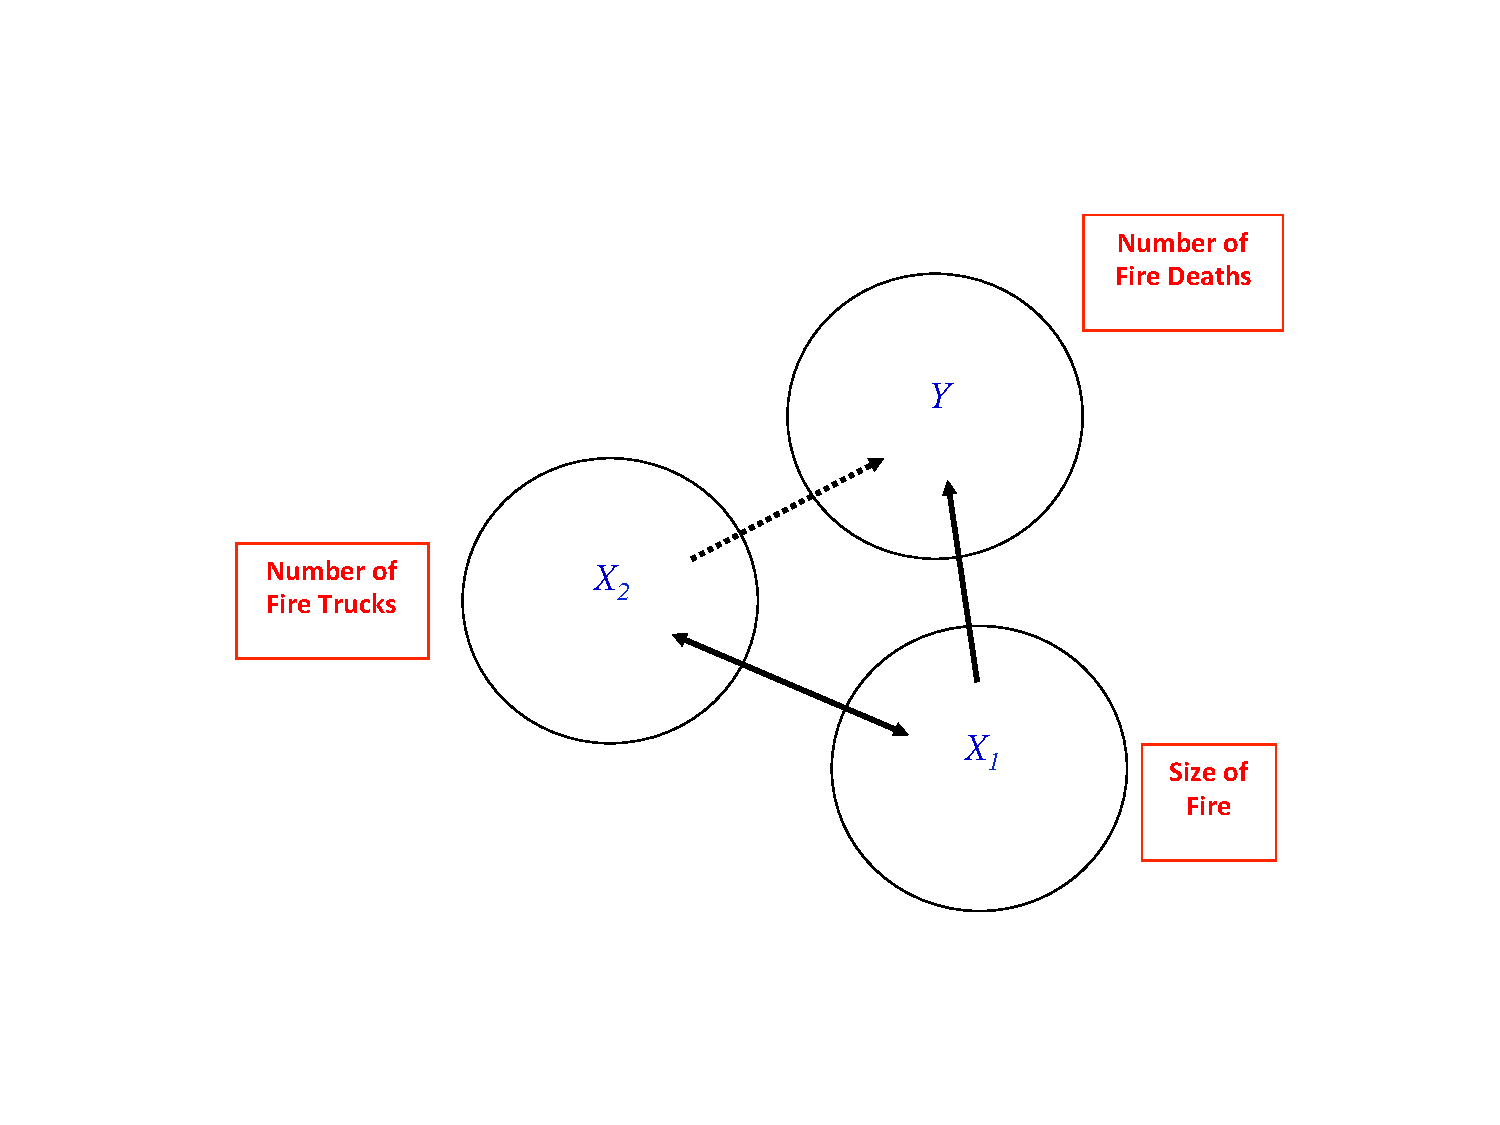
\includegraphics[width=5in]{12_LogicMult/spur.pdf}
  \caption{Spurious Relationships \label{fig:spur}}
\end{figure}

To control for spurious relationships, multiple regression accounts for the \textbf{partial effects} of one $X$ on another $X$. Partial effects deal with the shared variance between $Y$ and the $X$'s. This is illustrated in Figure \ref{fig:partef}.  In this example, the number of deaths resulting from house fires is positively associated with the number of fire trucks that are sent to the scene of the fire. A simple-minded analysis would conclude that if fewer trucks are sent, fewer fire-related deaths would occur. Of course, the number of trucks sent to the fire, and the number of 
fire-related deaths, are both driven by the magnitude of the fire. An appropriate control for the size of the fire would therefore presumably eliminate the positive association between the number of fire trucks at the scene and the number of deaths (and may even  reverse the direction of the relationship, as the larger number of trucks may more quickly suppress the fire).

\begin{figure}
  \centering
  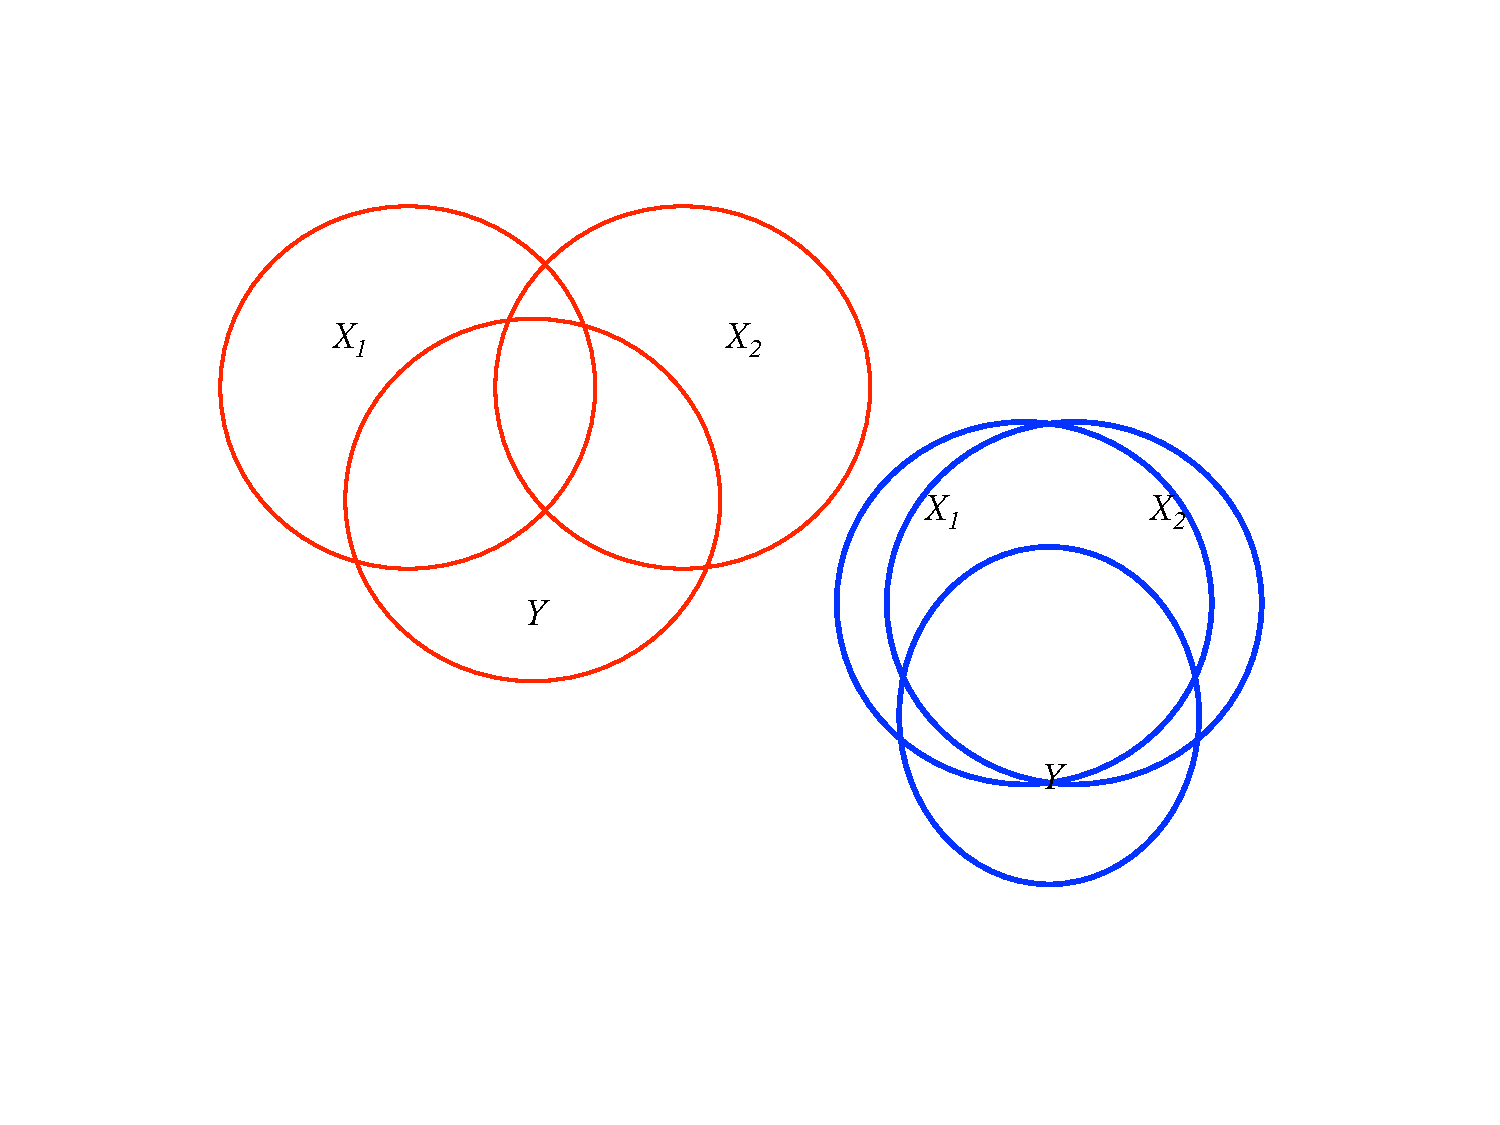
\includegraphics[width=5in]{12_LogicMult/partef.pdf}
  \caption{Partial Effects \label{fig:partef}}
\end{figure}

In Figure \ref{fig:partef}, the Venn diagram on the left shows a pair of $X$s that would jointly predict $Y$ better than either $X$ alone. However,
the overlapped area between $X_{1}$ and $X_{2}$ causes some confusion. That would need to be removed to estimate the ``pure" effect of $X_{1}$ on $Y$. The diagram on the right represents a dangerous case. Overall, $X_{1}$+$X_2$ explain $Y$ well, but we don`t know how the individual $X_1$ or $X_2$ influence $Y$.  This clouds our ability to see the effects of either of the $Xs$ on $Y$. In the extreme case of wholly overlapping explanations by the IVs, we face the condition of \textbf{multicolinearity} that makes estimation of the partial regression coefficients (the $Bs$) impossible.
     
In calculating the effect of $X_1$ on $Y$, we need to remove the effect of the other $X$’s on both $X_1$ and $Y$.  While multiple regression does this for us, we will walk through an example to illustrate the concepts. 

\begin{grbox}
\greybox{\textbf{Partial Effects} 

In a case with two IVs, $X_1$ and $X_2$
\begin{center}
  $Y = A + B_1X_{i1} + B_2X_{i2} + E_{i}$ 
\end{center}
\begin{itemize}
\item Remove the effect of $X_2$ and $Y$ 
\begin{center}
$\hat{Y_i} = A_1+B_1X_{i2}+E_{iY|X_{2}}$  
\end{center}
\item Remove the effect of $X_2$ on $X_1$: 
\begin{center}
$\hat{X_i} = A_2+B_2X_{i2}+E_{iX_{1}|X_{2}}$  
\end{center}
So,
\begin{center}
$E_{iY|X_{2}} = 0 + B_3E_{iX_{1}|X_{2}}$ \\
and \\
$B_3E_{iX_{1}|X_{2}} = B_1X_{i1}$  
\end{center}
\end{itemize}}
\end{grbox}

% example in R 
As an example, we will use age and ideology to predict perceived climate change risk. 

\begin{knitrout}
\definecolor{shadecolor}{rgb}{0.969, 0.969, 0.969}\color{fgcolor}\begin{kframe}
\begin{alltt}
\hlstd{ds.temp} \hlkwb{<-} \hlkwd{filter}\hlstd{(ds)} \hlopt \hlkwd{select}\hlstd{(glbcc_risk, ideol, age)} \hlopt
    \hlkwd{na.omit}\hlstd{()}

\hlstd{ols1} \hlkwb{<-} \hlkwd{lm}\hlstd{(glbcc_risk} \hlopt{~} \hlstd{ideol} \hlopt{+} \hlstd{age,} \hlkwc{data} \hlstd{= ds.temp)}
\hlkwd{summary}\hlstd{(ols1)}
\end{alltt}
\begin{verbatim}
## 
## Call:
## lm(formula = glbcc_risk ~ ideol + age, data = ds.temp)
## 
## Residuals:
##     Min      1Q  Median      3Q     Max 
## -8.7913 -1.6252  0.2785  1.4674  6.6075 
## 
## Coefficients:
##              Estimate Std. Error t value            Pr(>|t|)    
## (Intercept) 11.096064   0.244640  45.357 <0.0000000000000002 ***
## ideol       -1.042748   0.028674 -36.366 <0.0000000000000002 ***
## age         -0.004872   0.003500  -1.392               0.164    
## ---
## Signif. codes:  0 '***' 0.001 '**' 0.01 '*' 0.05 '.' 0.1 ' ' 1
## 
## Residual standard error: 2.479 on 2510 degrees of freedom
## Multiple R-squared:  0.3488,	Adjusted R-squared:  0.3483 
## F-statistic: 672.2 on 2 and 2510 DF,  p-value: < 0.00000000000000022
\end{verbatim}
\end{kframe}
\end{knitrout}

\noindent Note that the estimated coefficient for ideology is -1.0427478. To see how multiple regression removes the shared variance we first regress climate change risk on age and create an object \texttt{ols2.resids} of the residuals. 
\begin{knitrout}
\definecolor{shadecolor}{rgb}{0.969, 0.969, 0.969}\color{fgcolor}\begin{kframe}
\begin{alltt}
\hlstd{ols2} \hlkwb{<-} \hlkwd{lm}\hlstd{(glbcc_risk} \hlopt{~} \hlstd{age,} \hlkwc{data} \hlstd{= ds.temp)}
\hlkwd{summary}\hlstd{(ols2)}
\end{alltt}
\begin{verbatim}
## 
## Call:
## lm(formula = glbcc_risk ~ age, data = ds.temp)
## 
## Residuals:
##     Min      1Q  Median      3Q     Max 
## -6.4924 -2.1000  0.0799  2.5376  4.5867 
## 
## Coefficients:
##              Estimate Std. Error t value             Pr(>|t|)    
## (Intercept)  6.933835   0.267116  25.958 < 0.0000000000000002 ***
## age         -0.016350   0.004307  -3.796              0.00015 ***
## ---
## Signif. codes:  0 '***' 0.001 '**' 0.01 '*' 0.05 '.' 0.1 ' ' 1
## 
## Residual standard error: 3.062 on 2511 degrees of freedom
## Multiple R-squared:  0.005706,	Adjusted R-squared:  0.00531 
## F-statistic: 14.41 on 1 and 2511 DF,  p-value: 0.0001504
\end{verbatim}
\begin{alltt}
\hlstd{ols2.resids} \hlkwb{<-} \hlstd{ols2}\hlopt{$}\hlstd{residuals}
\end{alltt}
\end{kframe}
\end{knitrout}

Note that, when modeled alone, the estimated effect of age on glbccrsk is larger (-0.0164) than it was in the multiple regression with ideology (-0.00487). This is because age is correlated with ideology, and -- because ideology is also related to glbccrsk -- when we don't ``control for" ideology the age variable carries some of the influence of ideology.

\noindent Next, we regress ideology on age and create an object of the residuals. 
\begin{knitrout}
\definecolor{shadecolor}{rgb}{0.969, 0.969, 0.969}\color{fgcolor}\begin{kframe}
\begin{alltt}
\hlstd{ols3} \hlkwb{<-} \hlkwd{lm}\hlstd{(ideol} \hlopt{~} \hlstd{age,} \hlkwc{data} \hlstd{= ds.temp)}
\hlkwd{summary}\hlstd{(ols3)}
\end{alltt}
\begin{verbatim}
## 
## Call:
## lm(formula = ideol ~ age, data = ds.temp)
## 
## Residuals:
##     Min      1Q  Median      3Q     Max 
## -3.9492 -0.8502  0.2709  1.3480  2.7332 
## 
## Coefficients:
##             Estimate Std. Error t value             Pr(>|t|)    
## (Intercept) 3.991597   0.150478  26.526 < 0.0000000000000002 ***
## age         0.011007   0.002426   4.537           0.00000598 ***
## ---
## Signif. codes:  0 '***' 0.001 '**' 0.01 '*' 0.05 '.' 0.1 ' ' 1
## 
## Residual standard error: 1.725 on 2511 degrees of freedom
## Multiple R-squared:  0.00813,	Adjusted R-squared:  0.007735 
## F-statistic: 20.58 on 1 and 2511 DF,  p-value: 0.000005981
\end{verbatim}
\begin{alltt}
\hlstd{ols3.resids} \hlkwb{<-} \hlstd{ols3}\hlopt{$}\hlstd{residuals}
\end{alltt}
\end{kframe}
\end{knitrout}

\noindent Finally, we regress the residuals from ols2 on the residuals from ols3. Note that this regression does not include an intercept term. 
\begin{knitrout}
\definecolor{shadecolor}{rgb}{0.969, 0.969, 0.969}\color{fgcolor}\begin{kframe}
\begin{alltt}
\hlstd{ols4} \hlkwb{<-} \hlkwd{lm}\hlstd{(ols2.resids} \hlopt{~} \hlnum{0} \hlopt{+} \hlstd{ols3.resids)}
\hlkwd{summary}\hlstd{(ols4)}
\end{alltt}
\begin{verbatim}
## 
## Call:
## lm(formula = ols2.resids ~ 0 + ols3.resids)
## 
## Residuals:
##     Min      1Q  Median      3Q     Max 
## -8.7913 -1.6252  0.2785  1.4674  6.6075 
## 
## Coefficients:
##             Estimate Std. Error t value            Pr(>|t|)    
## ols3.resids -1.04275    0.02866  -36.38 <0.0000000000000002 ***
## ---
## Signif. codes:  0 '***' 0.001 '**' 0.01 '*' 0.05 '.' 0.1 ' ' 1
## 
## Residual standard error: 2.478 on 2512 degrees of freedom
## Multiple R-squared:  0.3451,	Adjusted R-squared:  0.3448 
## F-statistic:  1324 on 1 and 2512 DF,  p-value: < 0.00000000000000022
\end{verbatim}
\end{kframe}
\end{knitrout}

As shown, the estimated $B$ for $E_{iX_{1}|X_{2}}$, matches the estimated $B$ for ideology in the first regression. What we have done, and what multiple regression does, is ``clean" both $Y$ and $X_1$ (ideology) of their correlations with $X_2$ (age) by using the residuals from the bivariate regressions.
 
\section{Multiple Regression Example}



In this section, we walk through another example of multiple regression. First, we start with our two IV model. 
\begin{knitrout}
\definecolor{shadecolor}{rgb}{0.969, 0.969, 0.969}\color{fgcolor}\begin{kframe}
\begin{alltt}
\hlstd{ols1} \hlkwb{<-} \hlkwd{lm}\hlstd{(glbcc_risk} \hlopt{~} \hlstd{age} \hlopt{+} \hlstd{ideol,} \hlkwc{data} \hlstd{= ds.temp)}
\hlkwd{summary}\hlstd{(ols1)}
\end{alltt}
\begin{verbatim}
## 
## Call:
## lm(formula = glbcc_risk ~ age + ideol, data = ds.temp)
## 
## Residuals:
##     Min      1Q  Median      3Q     Max 
## -8.7913 -1.6252  0.2785  1.4674  6.6075 
## 
## Coefficients:
##              Estimate Std. Error t value            Pr(>|t|)    
## (Intercept) 11.096064   0.244640  45.357 <0.0000000000000002 ***
## age         -0.004872   0.003500  -1.392               0.164    
## ideol       -1.042748   0.028674 -36.366 <0.0000000000000002 ***
## ---
## Signif. codes:  0 '***' 0.001 '**' 0.01 '*' 0.05 '.' 0.1 ' ' 1
## 
## Residual standard error: 2.479 on 2510 degrees of freedom
## Multiple R-squared:  0.3488,	Adjusted R-squared:  0.3483 
## F-statistic: 672.2 on 2 and 2510 DF,  p-value: < 0.00000000000000022
\end{verbatim}
\end{kframe}
\end{knitrout}

The results show that the relationship between age and perceived risk (glbccrsk) is negative and insignificant. The relationship between ideology and perceived risk is also negative and significant. The coefficients of the $X$'s are interpreted in the same way as with simple regression, except that we are now controlling for the effect of the other $X$'s by removing their influence on the estimated coefficient. Therefore, we say that as ideology increases one unit, perceptions of the risk of climate change (glbccrsk) decrease by -1.0427478, controlling for the effect of age.  

As was the case with simple regression, multiple regression finds the intercept and slopes that minimize the sum of the squared residuals. With only one IV the relationship can be represented in a two-dimensional plane (a graph) as a line, but each IV adds another dimension. Two IVs create a regression plane within a cube, as shown in Figure \ref{fig:scatols}. The Figure shows a scatterplot of GCC risk, age, and ideology coupled with the regression plane. Note that this is a sample of 200 observations from the larger data set. Were we to add more IVs, we would generate a hypercube... and we haven't found a clever way to draw that yet.



\begin{figure}
  \centering
  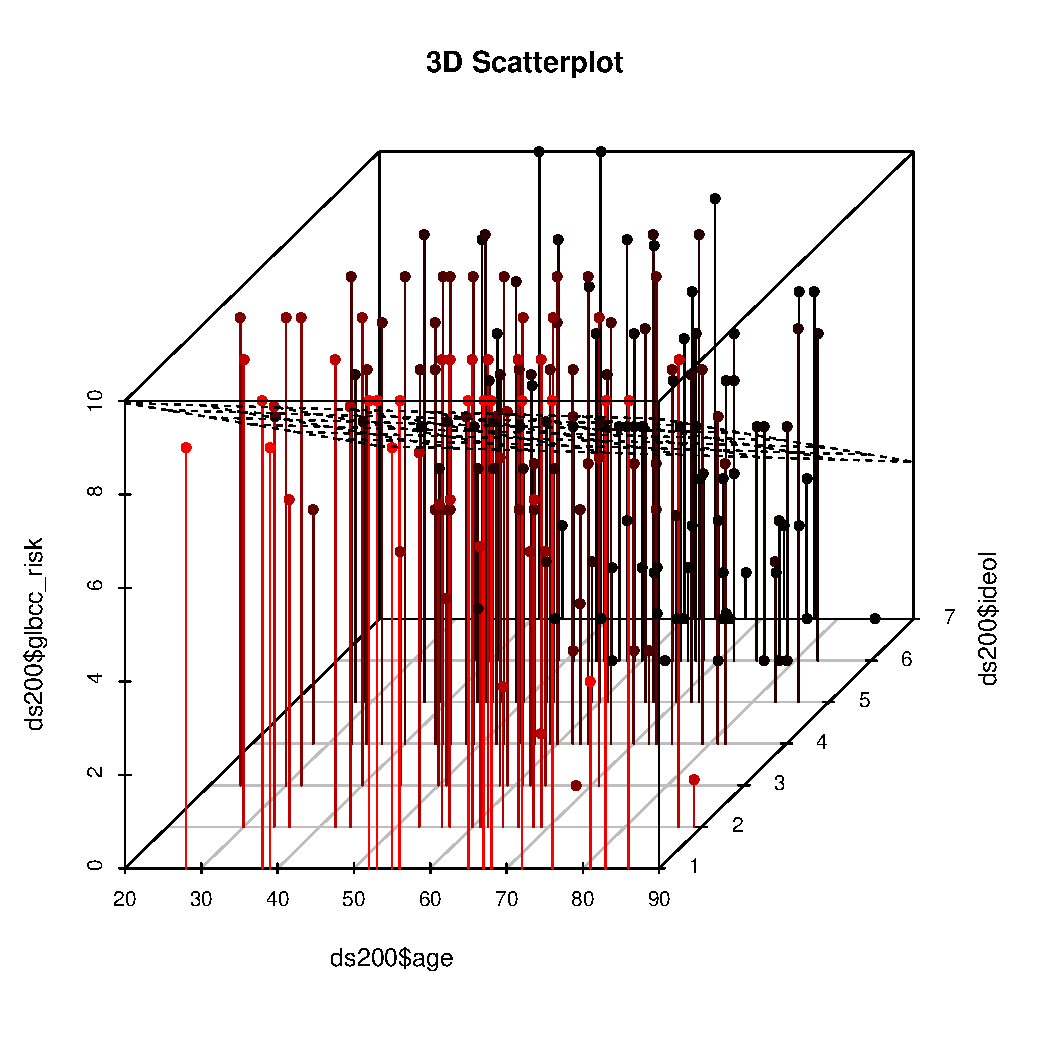
\includegraphics[width=4in]{12_LogicMult/scatols.pdf}%filename
  \caption{Scatterplot and Regression Plane of gcc risk, age, and
    ideology \label{fig:scatols}}
\end{figure}

In the next example education is added to the model. 

\begin{knitrout}
\definecolor{shadecolor}{rgb}{0.969, 0.969, 0.969}\color{fgcolor}\begin{kframe}
\begin{alltt}
\hlstd{ds.temp} \hlkwb{<-} \hlkwd{filter}\hlstd{(ds)} \hlopt \hlkwd{select}\hlstd{(glbcc_risk, age, education,}
    \hlstd{income, ideol)} \hlopt \hlkwd{na.omit}\hlstd{()}

\hlstd{ols2} \hlkwb{<-} \hlkwd{lm}\hlstd{(glbcc_risk} \hlopt{~} \hlstd{age} \hlopt{+} \hlstd{education} \hlopt{+} \hlstd{ideol,} \hlkwc{data} \hlstd{= ds.temp)}
\hlkwd{summary}\hlstd{(ols2)}
\end{alltt}
\begin{verbatim}
## 
## Call:
## lm(formula = glbcc_risk ~ age + education + ideol, data = ds.temp)
## 
## Residuals:
##     Min      1Q  Median      3Q     Max 
## -8.8092 -1.6355  0.2388  1.4279  6.6334 
## 
## Coefficients:
##              Estimate Std. Error t value            Pr(>|t|)    
## (Intercept) 10.841669   0.308416  35.153 <0.0000000000000002 ***
## age         -0.003246   0.003652  -0.889               0.374    
## education    0.036775   0.028547   1.288               0.198    
## ideol       -1.044827   0.029829 -35.027 <0.0000000000000002 ***
## ---
## Signif. codes:  0 '***' 0.001 '**' 0.01 '*' 0.05 '.' 0.1 ' ' 1
## 
## Residual standard error: 2.437 on 2268 degrees of freedom
## Multiple R-squared:  0.3607,	Adjusted R-squared:  0.3598 
## F-statistic: 426.5 on 3 and 2268 DF,  p-value: < 0.00000000000000022
\end{verbatim}
\end{kframe}
\end{knitrout}

We see that as a respondent's education increases one unit on the education scale, perceived risk appears to increase by 0.0367752, keeping age and ideology constant. However, this result is not significant. In the final example income is added to the model. Note that the size and  significance of education actually increases once income is included, indicating that education only has  bearing on the perceived risks of climate change once the independent effect of income is considered.

\begin{knitrout}
\definecolor{shadecolor}{rgb}{0.969, 0.969, 0.969}\color{fgcolor}\begin{kframe}
\begin{alltt}
\hlkwd{options}\hlstd{(}\hlkwc{scipen} \hlstd{=} \hlnum{999}\hlstd{)}  \hlcom{#to turn off scientific notation}
\hlstd{ols3} \hlkwb{<-} \hlkwd{lm}\hlstd{(glbcc_risk} \hlopt{~} \hlstd{age} \hlopt{+} \hlstd{education} \hlopt{+} \hlstd{income} \hlopt{+} \hlstd{ideol,} \hlkwc{data} \hlstd{= ds.temp)}
\hlkwd{summary}\hlstd{(ols3)}
\end{alltt}
\begin{verbatim}
## 
## Call:
## lm(formula = glbcc_risk ~ age + education + income + ideol, data = ds.temp)
## 
## Residuals:
##     Min      1Q  Median      3Q     Max 
## -8.7991 -1.6654  0.2246  1.4437  6.5968 
## 
## Coefficients:
##                  Estimate    Std. Error t value             Pr(>|t|)    
## (Intercept) 10.9232861851  0.3092149750  35.326 < 0.0000000000000002 ***
## age         -0.0044231931  0.0036688855  -1.206              0.22810    
## education    0.0632823391  0.0299443094   2.113              0.03468 *  
## income      -0.0000026033  0.0000009021  -2.886              0.00394 ** 
## ideol       -1.0366154295  0.0299166747 -34.650 < 0.0000000000000002 ***
## ---
## Signif. codes:  0 '***' 0.001 '**' 0.01 '*' 0.05 '.' 0.1 ' ' 1
## 
## Residual standard error: 2.433 on 2267 degrees of freedom
## Multiple R-squared:  0.363,	Adjusted R-squared:  0.3619 
## F-statistic:   323 on 4 and 2267 DF,  p-value: < 0.00000000000000022
\end{verbatim}
\end{kframe}
\end{knitrout}

\subsection{Hypothesis Testing and $t$-tests}

The logic of hypothesis testing with multiple regression is a straightforward extension from  simple regression as described in Chapter 7. Below we will demonstrate how to use the standard error of the ideology variable to test whether ideology influences perceptions of the perceived risk of global climate change. Specifically, we posit:
\begin{quote}
{$H_1$}: As respondents become more conservative, they will perceive climate change to be less risky, all else equal. 
\end{quote}
Therefore, $\beta_{ideology} < 0$. The null
hypothesis is that $\beta_{ideology} = 0$. 

To test $H_1$ we first need to find the standard error of the $B$ for ideology, ($B_j$).  
\begin{equation}
  SE(B_j) = \frac{S_E}{\sqrt{RSS_j}} 
\end{equation}
\noindent where $RSS_j =$ the residual sum of squares from the regression of $X_j$ (ideology) on the other $X$s (age, education, income) in the model. $RSS_j$ captures all of the \textbf{independent} variation in $X_j$. Note that the bigger $RSS_j$, the smaller $SE(B_j)$, and the smaller $SE(B_j)$, the more precise the estimate of $B_j$.
 
$S_E$ (the standard error of the model) is:
\begin{equation*}
 S_E = \sqrt{\frac{RSS}{n-k-1}}
\end{equation*}

We can use \texttt{R} to find the $RSS$ for ideology in our model. First we find the $S_E$ of the model: 
\begin{knitrout}
\definecolor{shadecolor}{rgb}{0.969, 0.969, 0.969}\color{fgcolor}\begin{kframe}
\begin{alltt}
\hlstd{Se} \hlkwb{<-} \hlkwd{sqrt}\hlstd{((}\hlkwd{sum}\hlstd{(ols3}\hlopt{$}\hlstd{residuals}\hlopt{^}\hlnum{2}\hlstd{))}\hlopt{/}\hlstd{(}\hlkwd{length}\hlstd{(ds.temp}\hlopt{$}\hlstd{ideol)} \hlopt{-} \hlnum{5} \hlopt{-}
    \hlnum{1}\hlstd{))}
\hlstd{Se}
\end{alltt}
\begin{verbatim}
## [1] 2.43312
\end{verbatim}
\end{kframe}
\end{knitrout}
Then we find the $RSS$, for ideology:
\begin{knitrout}
\definecolor{shadecolor}{rgb}{0.969, 0.969, 0.969}\color{fgcolor}\begin{kframe}
\begin{alltt}
\hlstd{ols4} \hlkwb{<-} \hlkwd{lm}\hlstd{(ideol} \hlopt{~} \hlstd{age} \hlopt{+} \hlstd{education} \hlopt{+} \hlstd{income,} \hlkwc{data} \hlstd{= ds.temp)}
\hlkwd{summary}\hlstd{(ols4)}
\end{alltt}
\begin{verbatim}
## 
## Call:
## lm(formula = ideol ~ age + education + income, data = ds.temp)
## 
## Residuals:
##     Min      1Q  Median      3Q     Max 
## -4.2764 -1.1441  0.2154  1.4077  3.1288 
## 
## Coefficients:
##                  Estimate    Std. Error t value             Pr(>|t|)    
## (Intercept)  4.5945481422  0.1944108986  23.633 < 0.0000000000000002 ***
## age          0.0107541759  0.0025652107   4.192   0.0000286716948757 ***
## education   -0.1562812154  0.0207596525  -7.528   0.0000000000000738 ***
## income       0.0000028680  0.0000006303   4.550   0.0000056434561990 ***
## ---
## Signif. codes:  0 '***' 0.001 '**' 0.01 '*' 0.05 '.' 0.1 ' ' 1
## 
## Residual standard error: 1.707 on 2268 degrees of freedom
## Multiple R-squared:  0.034,	Adjusted R-squared:  0.03272 
## F-statistic:  26.6 on 3 and 2268 DF,  p-value: < 0.00000000000000022
\end{verbatim}
\begin{alltt}
\hlstd{RSSideol} \hlkwb{<-} \hlkwd{sum}\hlstd{(ols4}\hlopt{$}\hlstd{residuals}\hlopt{^}\hlnum{2}\hlstd{)}
\hlstd{RSSideol}
\end{alltt}
\begin{verbatim}
## [1] 6611.636
\end{verbatim}
\end{kframe}
\end{knitrout}
Finally, we calculate the $SE$ for ideology:
\begin{knitrout}
\definecolor{shadecolor}{rgb}{0.969, 0.969, 0.969}\color{fgcolor}\begin{kframe}
\begin{alltt}
\hlstd{SEideol} \hlkwb{<-} \hlstd{Se}\hlopt{/}\hlkwd{sqrt}\hlstd{(RSSideol)}
\hlstd{SEideol}
\end{alltt}
\begin{verbatim}
## [1] 0.02992328
\end{verbatim}
\end{kframe}
\end{knitrout}

Once the $SE(B_j)$ is known, the $t$-test for the ideology coefficient
can be calculated. The $t$ value is the ratio of the estimated
coefficient to its standard error. 
\begin{equation}
  t = \frac{B_j}{SE(B_j)}
\end{equation}

This can be calculated using \texttt{R}. 
\begin{knitrout}
\definecolor{shadecolor}{rgb}{0.969, 0.969, 0.969}\color{fgcolor}\begin{kframe}
\begin{alltt}
\hlstd{ols3}\hlopt{$}\hlstd{coef[}\hlnum{5}\hlstd{]}\hlopt{/}\hlstd{SEideol}
\end{alltt}
\begin{verbatim}
##     ideol 
## -34.64245
\end{verbatim}
\end{kframe}
\end{knitrout}

As we see, the result is statistically significant, and therefore we reject the null hypothesis.  Also note that the results match those from the \texttt{R} output for the full model, as was shown earlier.

\section{Summary}
The use of multiple regression, when compared to simple bivariate regression, allows for more sophisticated and interesting analyses. The most important feature is the ability of the analyst (that's you!) to statistically control for the effects of all other IVs when estimating any $B$.
In essence, we ``clean" the estimated relationship between any $X$ and $Y$ of the influence of all  other $Xs$ in the model. Hypothesis testing in multiple regression requires that we identify the independent variation in each $X$, but otherwise the estimated standard error for each $B$ is analogous to that for simple regression.

So, maybe it's a little more complicated. But look at what we can observe! Our estimates from the examples in this chapter show that age, income and education are all related to political ideology, but even when we control for their effects, ideology retains a potent influence on the perceived
risks of climate change. Politics matters.








\chapter{Multiple Regression and Model Building} 

This book focuses on the use of systematic quantitative analysis for purposes of building, refining and testing theoretical propositions in the policy and social sciences. All of the tools discussed so far -- including univariate, bi-variate, and simple regression analysis -- provide means to evaluate distributions and test hypotheses concerning simple relationships. Most policy and social theories,  however, include multiple explanatory variables. \textit{Multiple regression} extends the utility of simple regression by permitting the inclusion of two or more explanatory variables.  This chapter discusses strategies for determining what variables to include (or exclude) in the model.  As before, we use the \texttt{tbur} data.  

\section{Model Building}

Model building is the process of deciding which independent variables to include in the model.\footnote{Model building also concerns decisions about model functional form, which we address in the next chapter.} For our purposes, when deciding which variables to include, theory and findings from the extant literature should be the most prominent guides. Apart from theory, however, this chapter examines empirical strategies that can help determine if the addition of new variables improves overall model fit. In general, when adding a variable check for: a) improved prediction based on empirical indicators, b) statistically and substantively significant estimated coefficients, and c) stability of model coefficients---do other coefficients change when adding the new one -- particularly look for sign changes.  

\subsection{Theory and Hypotheses}

The most important guidance for deciding whether a variable (or variables) should be included in your model is provided by theory and prior research. Simply put, knowing the literature on your topic is vital to knowing what variables are important. You should be able to articulate a clear theoretical reason for including each variable in your model. In those cases where you don't have much theoretical guidance, however, you should use model \textit{parsimony}, which is a function of simplicity and model fit, as your guide. You can focus on whether the inclusion of a variable improves model fit.  In the next section, we will explore several empirical indicators that can be used to evaluate the appropriateness of inclusion of variables. 

\subsection{Empirical Indicators}

When building a model, it is best to start with a few IV's and then begin adding other variables. However, when adding a variable, check for: 
\begin{enumerate}
\item Improved prediction (increase in adjusted $R^2$)
\item Statistically and substantively significant estimated coefficients
\item Stability of model coefficients
  \begin{itemize}
\item Do other coefficients change when adding the new one?
\item Particularly look for sign changes for estimated coefficients.
  \end{itemize}
  \end{enumerate}

\subsubsection{Coefficient of Determination: $R^2$}

$R^2$ was previously discussed within the context of simple regression. The extension to multiple regression is straightforward, except that multiple regression leads us to place greater weight on the use of the \textbf{adjusted $R^2$}. Recall that the adjusted $R^2$ corrects for the inclusion of multiple independent variables; $R^{2}$ is the ratio of the explained sum of squares to the total sum of squares (\textit{ESS/TSS}). The components of $R^{2}$ for an observation are illustrated in Figure \ref{fig:rsq}. As before, for each observation $Y_{i}$, variation around the mean can be decomposed into that which is ``explained" by the regression model and that which is not.  
\begin{figure}
  \centering
  \includegraphics[width=5in]{13_ModelFit/rsquared.pdf}
  \caption[$R^{2}$]{ \label{fig:rsq}}
\end{figure}

$R^2$ is expressed as: 
\begin{equation}
 R^{2} = 1-\frac{RSS}{TSS}  
\end{equation}

However, this formulation of $R^2$ is insensitive to the complexity of the model and the degrees of freedom provided by your data. This means that an increase in the number of $k$ independent variables, can increase the $R^2$. Adjusted $R^2$ penalizes the $R^2$ by correcting for the degrees of freedom. It is defined as: 
\begin{equation}
 \text{adjusted} R^2 = 1-\frac{\frac{RSS}{n-k-1}}{\frac{TSS}{n-k-1}}
\end{equation}

The $R^2$ of two models can be compared, as illustrated by the following example. The first (simpler) model consists of basic demographics (age, education, and income) as predictors of climate change risk. The second (more complex) model adds the variable measuring political ideology to the explanation.


\begin{knitrout}
\definecolor{shadecolor}{rgb}{0.969, 0.969, 0.969}\color{fgcolor}\begin{kframe}
\begin{alltt}
\hlstd{ds.temp} \hlkwb{<-} \hlkwd{filter}\hlstd{(ds)} \hlopt \hlkwd{select}\hlstd{(glbcc_risk, age, education,}
    \hlstd{income, ideol)} \hlopt \hlkwd{na.omit}\hlstd{()}

\hlstd{ols1} \hlkwb{<-} \hlkwd{lm}\hlstd{(glbcc_risk} \hlopt{~} \hlstd{age} \hlopt{+} \hlstd{education} \hlopt{+} \hlstd{income,} \hlkwc{data} \hlstd{= ds.temp)}
\hlkwd{summary}\hlstd{(ols1)}
\end{alltt}
\begin{verbatim}
## 
## Call:
## lm(formula = glbcc_risk ~ age + education + income, data = ds.temp)
## 
## Residuals:
##     Min      1Q  Median      3Q     Max 
## -6.9189 -2.0546  0.0828  2.5823  5.1908 
## 
## Coefficients:
##                 Estimate   Std. Error t value             Pr(>|t|)    
## (Intercept)  6.160506689  0.342491831  17.987 < 0.0000000000000002 ***
## age         -0.015571138  0.004519107  -3.446              0.00058 ***
## education    0.225285858  0.036572082   6.160       0.000000000858 ***
## income      -0.000005576  0.000001110  -5.022       0.000000551452 ***
## ---
## Signif. codes:  0 '***' 0.001 '**' 0.01 '*' 0.05 '.' 0.1 ' ' 1
## 
## Residual standard error: 3.008 on 2268 degrees of freedom
## Multiple R-squared:  0.02565,	Adjusted R-squared:  0.02437 
## F-statistic: 19.91 on 3 and 2268 DF,  p-value: 0.0000000000009815
\end{verbatim}
\begin{alltt}
\hlstd{ols2} \hlkwb{<-} \hlkwd{lm}\hlstd{(glbcc_risk} \hlopt{~} \hlstd{age} \hlopt{+} \hlstd{education} \hlopt{+} \hlstd{income} \hlopt{+} \hlstd{ideol,} \hlkwc{data} \hlstd{= ds.temp)}
\hlkwd{summary}\hlstd{(ols2)}
\end{alltt}
\begin{verbatim}
## 
## Call:
## lm(formula = glbcc_risk ~ age + education + income + ideol, data = ds.temp)
## 
## Residuals:
##     Min      1Q  Median      3Q     Max 
## -8.7991 -1.6654  0.2246  1.4437  6.5968 
## 
## Coefficients:
##                  Estimate    Std. Error t value             Pr(>|t|)    
## (Intercept) 10.9232861851  0.3092149750  35.326 < 0.0000000000000002 ***
## age         -0.0044231931  0.0036688855  -1.206              0.22810    
## education    0.0632823391  0.0299443094   2.113              0.03468 *  
## income      -0.0000026033  0.0000009021  -2.886              0.00394 ** 
## ideol       -1.0366154295  0.0299166747 -34.650 < 0.0000000000000002 ***
## ---
## Signif. codes:  0 '***' 0.001 '**' 0.01 '*' 0.05 '.' 0.1 ' ' 1
## 
## Residual standard error: 2.433 on 2267 degrees of freedom
## Multiple R-squared:  0.363,	Adjusted R-squared:  0.3619 
## F-statistic:   323 on 4 and 2267 DF,  p-value: < 0.00000000000000022
\end{verbatim}
\end{kframe}
\end{knitrout}
As can be seen by comparing the model results, the more complex model that includes political ideology has a higher $R^2$ than does the simpler model. This indicates that the more complex model explains a greater fraction of the variance in perceived risks of climate change. However, we don't know if this improvement is statistically significant. In order to determine whether the more complex model adds significantly to the explanation of perceive risks, we can utilize the $F$-test.  

\subsubsection{$F$-test}

The $F$-test is a test statistic based on the $F$ distribution, in the same way the the $t$-test is based on the $t$ distribution. The $F$ distribution skews right and ranges between $0$ and $\infty$. Just like the $t$ distribution, the $F$ distribution approaches normal as the degrees of freedom increase.\footnote{Note that the $F$ distribution is the square of a $t$-distributed variable with $m$ degrees of freedom. The $F$ distribution has $1$ degree of freedom in the numerator and $m$ degrees of in the denominator: 
\begin{equation*}
  t^2_m = F_{1,m} 
\end{equation*}}

$F$-tests are used to test for the statistical significance of the overall model fit. The null hypothesis for an $F$-test is that the model offers no improvement for predicting $Y_i$ over the mean of $Y$,
$\bar{Y}$. 

The formula for the $F$-test is: 

\begin{equation}
  F = \frac{\frac{ESS}{k}}{\frac{RSS}{n-k-1}}
\end{equation}

\noindent where $k$ is the number of parameters and $n-k-1$ are the degrees of freedom. Therefore, $F$ is a ratio of the explained variance to the residual variance, correcting for the number of observations and parameters. The $F$-value is compared to the $F$-distribution, just like a $t$-distribution, to obtain a $p$-value. Note that the \texttt{R} output includes the $F$ statistic and $p$ value. 

\subsubsection{Nested $F$-test}

For model building we turn to the nested $F$-test, which tests whether a more complex model (with more IVs) adds to the explanatory power over a simpler model (with fewer IVs). To find out, we calculate an F-statistic for the model improvement: 

\begin{equation}
  F = \frac{\frac{ESS_1-ESS_0}{q}}{\frac{RSS_1}{n-k-1}}
\end{equation}

\noindent where $q$ is the difference in the number of IVs between the simpler and the mode complex models.  The complex model has $k$ IVs (and estimates $k$ parameters), and the simpler model has $k-q$ IVs (and estimates only $k-q$ parameters). $ESS_1$ is the explained sum of squares
for the complex model. $RSS_1$ is the residual sum of squares for the complex model. $ESS_0$ is the explained sum of squares for the simpler
model. So the nested-F represents the ratio of the additional explanation per added IV, over the residual sum of squares divided by the model degrees of freedom.

We can use \texttt{R}, to calculate the $F$ statistic based on our previous example.  
\begin{knitrout}
\definecolor{shadecolor}{rgb}{0.969, 0.969, 0.969}\color{fgcolor}\begin{kframe}
\begin{alltt}
\hlstd{TSS} \hlkwb{<-} \hlkwd{sum}\hlstd{((ds.temp}\hlopt{$}\hlstd{glbcc_risk} \hlopt{-} \hlkwd{mean}\hlstd{(ds.temp}\hlopt{$}\hlstd{glbcc_risk))}\hlopt{^}\hlnum{2}\hlstd{)}
\hlstd{TSS}
\end{alltt}
\begin{verbatim}
## [1] 21059.86
\end{verbatim}
\begin{alltt}
\hlstd{RSS.mod1} \hlkwb{<-} \hlkwd{sum}\hlstd{(ols1}\hlopt{$}\hlstd{residuals}\hlopt{^}\hlnum{2}\hlstd{)}
\hlstd{RSS.mod1}
\end{alltt}
\begin{verbatim}
## [1] 20519.57
\end{verbatim}
\begin{alltt}
\hlstd{ESS.mod1} \hlkwb{<-} \hlstd{TSS} \hlopt{-} \hlstd{RSS.mod1}
\hlstd{ESS.mod1}
\end{alltt}
\begin{verbatim}
## [1] 540.2891
\end{verbatim}
\begin{alltt}
\hlstd{RSS.mod2} \hlkwb{<-} \hlkwd{sum}\hlstd{(ols2}\hlopt{$}\hlstd{residuals}\hlopt{^}\hlnum{2}\hlstd{)}
\hlstd{RSS.mod2}
\end{alltt}
\begin{verbatim}
## [1] 13414.89
\end{verbatim}
\begin{alltt}
\hlstd{ESS.mod2} \hlkwb{<-} \hlstd{TSS} \hlopt{-} \hlstd{RSS.mod2}
\hlstd{ESS.mod2}
\end{alltt}
\begin{verbatim}
## [1] 7644.965
\end{verbatim}
\begin{alltt}
\hlstd{F} \hlkwb{<-} \hlstd{((ESS.mod2} \hlopt{-} \hlstd{ESS.mod1)}\hlopt{/}\hlnum{1}\hlstd{)}\hlopt{/}\hlstd{(RSS.mod2}\hlopt{/}\hlstd{(}\hlkwd{length}\hlstd{(ds.temp}\hlopt{$}\hlstd{glbcc_risk)} \hlopt{-}
    \hlnum{4} \hlopt{-} \hlnum{1}\hlstd{))}
\hlstd{F}
\end{alltt}
\begin{verbatim}
## [1] 1200.629
\end{verbatim}
\end{kframe}
\end{knitrout}
Or, you can simply use the \texttt{anova} function in $R$: 
\begin{knitrout}
\definecolor{shadecolor}{rgb}{0.969, 0.969, 0.969}\color{fgcolor}\begin{kframe}
\begin{alltt}
\hlkwd{anova}\hlstd{(ols1, ols2)}
\end{alltt}
\begin{verbatim}
## Analysis of Variance Table
## 
## Model 1: glbcc_risk ~ age + education + income
## Model 2: glbcc_risk ~ age + education + income + ideol
##   Res.Df   RSS Df Sum of Sq      F                Pr(>F)    
## 1   2268 20520                                              
## 2   2267 13415  1    7104.7 1200.6 < 0.00000000000000022 ***
## ---
## Signif. codes:  0 '***' 0.001 '**' 0.01 '*' 0.05 '.' 0.1 ' ' 1
\end{verbatim}
\end{kframe}
\end{knitrout}

\noindent As shown using both approaches, the inclusion of ideology significantly improves model fit. 

\subsection{Risks in Model Building}

As is true of most things in life, there are risks to consider when building statistical models. First, are you including irrelevant $X$'s? These can increase model complexity, reduce adjusted $R^2$, and  increase model variability across samples. Remember that you should have a theoretical basis for inclusion of all of the variables in your model. 

Second, are you omitting relevant $X$'s? Not including important variables can fail to capture fit and can bias other estimated coefficients, particularly when the omitted $X$ is related to both other $X$'s and to the dependent variable $Y$. 

Finally, remember that we are using sample data. Therefore, about 5\% of the time, our sample will include random observations of $X$'s that result in $B$'s that meet classical hypothesis tests -- resulting in a Type I error. Conversely, the $B$'s may be important, but the sample data will randomly include observations of $X$ that result in estimated parameters that do not meet  the classical statistical tests -- resulting in a Type II error.  That's why we rely on theory, prior hypotheses, and replication. 

\section{Evils of Stepwise Regression}

Almost all statistical software packages (including $R$) permit a number of mechanical ``search strategies" for finding IVs that make a statistically significant contribution to the prediction of the model dependent variable. The most common of these is called \texttt{stepwise regression}, which may also be referred to as forward, backward (or maybe even upside down!) stepwise regression. Stepwise procedures do not require that the analyst think -- you just have to designate a pool of possible IVs and let the package go to work, sifting through the IVs to identify those that (on the
basis of your sample data) appear to be related to the model dependent variable.  The stepwise procedures use sequential F-tests, sequentially adding variables that ``improve the fit" of the mindless model until there are no more IVs that meet some threshold (usually $p<0.05$) of statistical significance. These procedures are like mechanically wringing all of the explanation you can get for $Y$ out of some pool of $X$.

You should already recognize that these kind of methods pose serious problems. First and foremost, this is an atheoretical approach to model building. But, what if you have no theory to start with -- is a stepwise approach appropriate then? No, for several reasons. If any of the candidate $X$ variables are strongly correlated, the inclusion of the first one will ``use up" some of the explanation of the second, because of the way OLS calculates partial regression coefficients. For that reason, once one of the variables is mechanically selected, the other will tend to be excluded because it will have less to contribute to $Y$. Perhaps more damning, stepwise approaches as highly susceptible to inclusion of spuriously related variables. Recall that we are using samples, drawn from the larger population, and that samples are subject to random variation. If the step-wise process uses the classical 0.05 cut-off for inclusion of a variable, that means that one time in twenty (in the long run) we will include a variable that meets the criterion only by random chance.\footnote{Add to that the propensity of journals to publish articles that have new and exciting findings, in the form of statistically significant modeled coefficients, and you can see that there would be a substantial risk: that of finding and promoting nonsense findings.} Recall that the classical hypothesis test requires that we specify our hypothesis in advance; step-wise processes simply rummage around within a set of potential IVs to find those that fit.

There have been notable cases in which mechanical model building has resulted in seriously problematic ``findings" that have very costly implications for society. One is recounted in the PBS Frontline episode called ``Currents of Fear".\footnote{The program was written, produced  and directed by Jon Palfreman, and it was first broadcast on June 13, 1995. The full transcript can be found here: http://www.pbs.org/wgbh/pages/frontline/programs/transcripts/1319.html} The story concerns whether electromagnetic fields (EMFs) from technologies including high-voltage power lines cause cancer in people who are exposed. The problem was that ``cancer clusters" could be identified that were proximate to the power lines, but no laboratory experiments could find a connection. But concerned citizens and activists persisted in believing there was a causal relationship. In that context, the Swedish government sponsored a very ambitious study to settle the question. Here is the text of the discussion from  the Frontline program:

\begin{quote}
... in 1992, a landmark study appeared from Sweden. A huge investigation, it enrolled everyone  living within 300 meters of Sweden's high-voltage  transmission line system over a 25-year period.  They went far beyond all previous studies in their efforts to measure magnetic fields, calculating the fields that the children were exposed to at the time of their cancer diagnosis and before. This study  reported an apparently clear association between magnetic field exposure and childhood leukemia, with a risk ratio for the most highly exposed of nearly 4.

The Swedish government announced it was investigating new policy options, including whether to  move children away from schools near power lines. Surely, here was the proof that power lines were  dangerous, the proof that even the physicists and biological naysayers would have to accept. But three years after the study was published, the Swedish research no longer looks so unassailable. This is a  copy of the original contractor's report, which reveals the remarkable thoroughness of the Swedish team.  Unlike the published article, which just summarizes part of the data, the report shows everything they did in  great detail, all the things they measured and all the comparisons they made.

When scientists saw how many things they had measured -- nearly 800 risk ratios are in the report -- they began accusing the Swedes of falling into one of the most fundamental errors in epidemiology, sometimes called the multiple comparisons fallacy.
\end{quote}

So, according to the Frontline report, the Swedish EMF study regressed the incidence of nearly  800 possible cancers onto the proximity of its citizens to high-voltage power lines. In some cases, there appeared to be a positive relationship. These they reported. In other cases, there was no relationship, and in some the relationship was negative - which would seem to imply (if you were so silly as to do so) that living near the high voltage lines actually protected people from cancer. But only the positive relationships were included in the reports, leading to a false impression that the study had confirmed that proximity to high-voltage lines causes cancer. Embarrassing to the study authors, to put it mildly.

\section{Summary}

This chapter has focused on multiple regression model building. The keys to that process are understanding (a) the critical role of theory and prior research findings in model specification, and (b) the meaning of the partial regression coefficients produced by OLS. When theory is not well-developed, you can thoughtfully employ nested F-tests to evaluate whether the hypothesized inclusion of an $X$ variable meaningfully contributes to the explanation of $Y$. But you should avoid reliance on mechanical model-building routines, like step-wise regression, because these can lead you down into statistical perdition. None of us want to see that happen!







\chapter{Topics in Multiple Regression}


Thus far we have developed the basis for multiple OLS reression using matrix algebra, delved into the meaning of the estimated partial regression coefficient, and revisited the basis for hypothesis testing in OLS. In this chapter we turn to one of the key strengths of OLS: the robust flexibility of OLS for model specification. First we will discuss how to include binary variables (referred to as ``dummy variables") as IVs in an OLS model. Next ww will show you how to build on dummy variables to model their interactions with other variables in your model. Finally, we will address an alternative way to express the partial regression coefficients -- using standardized coefficients -- that permit you to compare the magnitudes of the estimated effects of your IVs even when they are measured on different scales. As has been our custom, the examples in this chapter are based on variable from the \texttt{tbur} data set.  

\section{Dummy Variables} 

Thus far, we have considered OLS models that include variables measured on interval level scales (or, in a pinch and with caution, ordinal scales). That is fine when we have variables for which we can develop valid and reliable interval (or ordinal) measures. But in the policy and social sciences we often want to include in our analysis concepts that do not readily admit to interval measure -- including many cases in which a variable has an ``on - off", or ``present - absent" quality. In other cases we want to include a concept that is essentially nominal in nature, such that an observation can be categorized as a subset but not measured on a ``high-low" or ``more-less" type of scale. In these instances we can utilize what is generally known as a dummy variable, but are also referred to as indicator variables, Boolean variables, or categorical variables.

\begin{grbox}
\greybox{\textbf{What the Heck are ``Dummy Variables"?}}

\begin{itemize}  
\item A dichotomous variable, with values of 0 and 1;
\item A value of 1 represents the presence of some quality, a zero its absence;
\item The 1s are compared to the 0s, who are known as the ``referent group";
\item Dummy variables are often thought of as a proxy for a qualitative variable.
\end{itemize}  
\end{grbox}

Dummy variables allow for tests of the differences in overall value of the $Y$ for different nominal groups in the data. They are akin to a difference of means test for the groups identified by the dummy variable. Dummy variables allow for comparisons between an included (the 1s) and an omitted (the 0s) group. Therefore, it is important to be clear about which group is omitted and serving as the ``comparison category." 

It is often the case that there are more than two groups, represented by a set of nominal categories. In that case, the variable will consist of two or more dummy variables, with 0/1 codes for each category except the referent group (which is omitted). Several examples of categorical variables that can be represented on multiple regression with dummy variables include:

\begin{itemize}
\item Experimental treatment and control groups (treatment=1, control=0)
\item Gender (male=1, female=0 or vice versa)
\item Race and ethnicity (a dummy for each group, with one omitted referent group)
\item Region of residence (dummy for each region with one omitted reference region)
\item Type of education (dummy for each type with omitted reference type)
\item Religious affiliation (dummy for each religious denomination with omitted reference)
\end{itemize}

The value of the dummy coefficient represents the estimated difference in $Y$ between the dummy group and the reference group. Because the estimated difference is the average over all of the $Y$ observations, the dummy is best understood as a change in the value of the intercept ($A$) for the ``dummied" group. This is illustrated in Figure \ref{fig:dum}. In this illustration, the value of $Y$  is a function of $X_1$ (a continuous variable) and $X_2$ (a dummy variable). When $X_2$ is equal to 0 (the referent case) the top regression line applies. When $X_2 = 1$, the value of $Y$ is reduced to the bottom line. In short, $X_2$ has a negative estimated partial regression coefficient represented by the difference in height between the two regression lines.

\begin{figure}
  \centering
  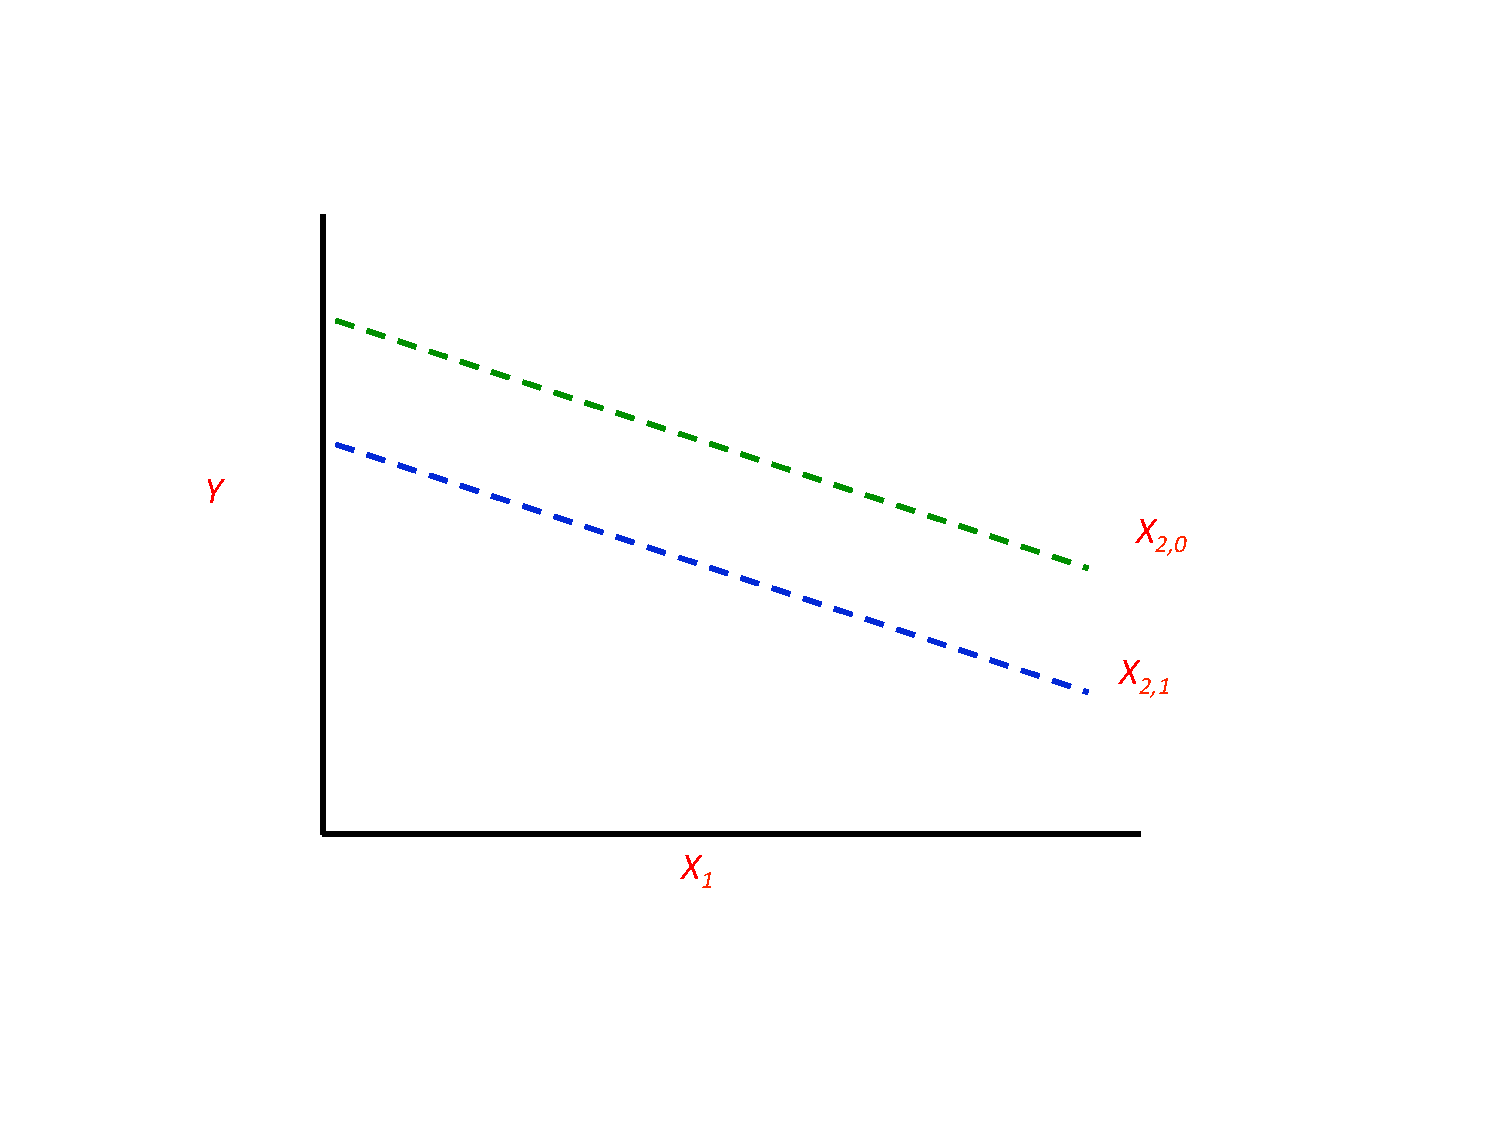
\includegraphics[width=5in]{14_Topics/dummy.pdf}%filename
  \caption{Dummy Intercept Variables \label{fig:dum}}
\end{figure}

For a case with multiple nominal categories (e.g., region) the procedure is as follows: (a) determine which category will be assigned as the referent group; (b) create a dummy variable for each of the other categories. For example, if you are coding a dummy for four regions (North, South, East and West), you could designate the South as the referent group. Then you would create dummies for the other three regions. Then, all observations from
the North would get a value of 1 in the North dummy, and zeros in all others. Similarly, East and West observations would receive a 1 in their respective dummy category and zeros elsewhere. The observations from the South region would be given values of zero in all three categories. The interpretation of the partial regression coefficients for each of the three dummies would then be the estimated difference in $Y$ between observations from the North, East and West and those from the South.

Now let's walk through an example of an $R$ model with a dummy variable and the interpretation of that model. We will predict climate change risk using age, education, income, ideology, and ``gend", a dummy variable for gender for which 1 = male and 0 = female. 


\begin{knitrout}
\definecolor{shadecolor}{rgb}{0.969, 0.969, 0.969}\color{fgcolor}\begin{kframe}
\begin{alltt}
\hlstd{ols1} \hlkwb{<-} \hlkwd{lm}\hlstd{(glbcc_risk} \hlopt{~} \hlstd{age} \hlopt{+} \hlstd{education} \hlopt{+} \hlstd{income} \hlopt{+} \hlstd{ideol} \hlopt{+} \hlstd{gender,}
    \hlkwc{data} \hlstd{= ds.temp)}
\hlkwd{summary}\hlstd{(ols1)}
\end{alltt}
\begin{verbatim}
## 
## Call:
## lm(formula = glbcc_risk ~ age + education + income + ideol + 
##     gender, data = ds.temp)
## 
## Residuals:
##     Min      1Q  Median      3Q     Max 
## -8.8976 -1.6553  0.1982  1.4814  6.7046 
## 
## Coefficients:
##                  Estimate    Std. Error t value             Pr(>|t|)    
## (Intercept) 10.9396287313  0.3092105590  35.379 < 0.0000000000000002 ***
## age         -0.0040621210  0.0036713524  -1.106              0.26865    
## education    0.0665255149  0.0299689664   2.220              0.02653 *  
## income      -0.0000023716  0.0000009083  -2.611              0.00908 ** 
## ideol       -1.0321209152  0.0299808687 -34.426 < 0.0000000000000002 ***
## gender      -0.2221178483  0.1051449213  -2.112              0.03475 *  
## ---
## Signif. codes:  0 '***' 0.001 '**' 0.01 '*' 0.05 '.' 0.1 ' ' 1
## 
## Residual standard error: 2.431 on 2265 degrees of freedom
## Multiple R-squared:  0.364,	Adjusted R-squared:  0.3626 
## F-statistic: 259.3 on 5 and 2265 DF,  p-value: < 0.00000000000000022
\end{verbatim}
\end{kframe}
\end{knitrout}
First note that the inclusion of the dummy variables doe not change the manner in which you interpret the other (non-dummy) variables in the model; the estimated partial regression coefficients for age, education, income and ideology should all be interpreted as described in the prior chapter. Note that the estimated partial regression coefficient for ``gender" is negative and statistically significant, indicating that males are less likely to be concerned about the environment than are females. The estimate indicates that, all else being equal, the average difference between men and women on the climate change risk scale is -0.2221178. 

%% in future editions I want to add a table showing how to code different kinds of dummy variables

\section{Interaction Effects}

Dummy variables can also be used to estimate the ways in which the effect of a variable differs across subsets of cases. These kinds of effects are generally called ``interactions".  When an interaction occurs, the effect of one $X$ is dependent on the value of another. Typically, an OLS model is additive, where the $B$'s are added together to predict $Y$; 

  $Y_i = A + BX_1 + BX_2 + BX_3 + BX_4 + E_i$. 
  
However, an interaction model has a multiplicative effect where two of the IVs are multiplied;

  $Y_i = A + BX_1 + BX_2 + BX_3 * BX_4 + E_i$. 

A ``slope dummy" is a special kind of interaction in which a dummy variable  is interacted with (multiplied by) a scale (ordinal or higher) variable. Suppose, for example, that you hypothesized that the effects of political of ideology on perceived risks of climate change were different for men and women. Perhaps men are more likely than women to consistently integrate ideology into climate change risk perceptions. In such a case, a dummy variable (0=women, 1=men) could be interacted with ideology (1=strong liberal, 7=strong conservative) to predict levels of perceived risk of climate change (0=no risk, 10=extreme risk).  If your hypothesized interaction was correct, you would observe the kind of pattern as shown in Figure \ref{fig:dumin}. 

\begin{figure}
  \centering
  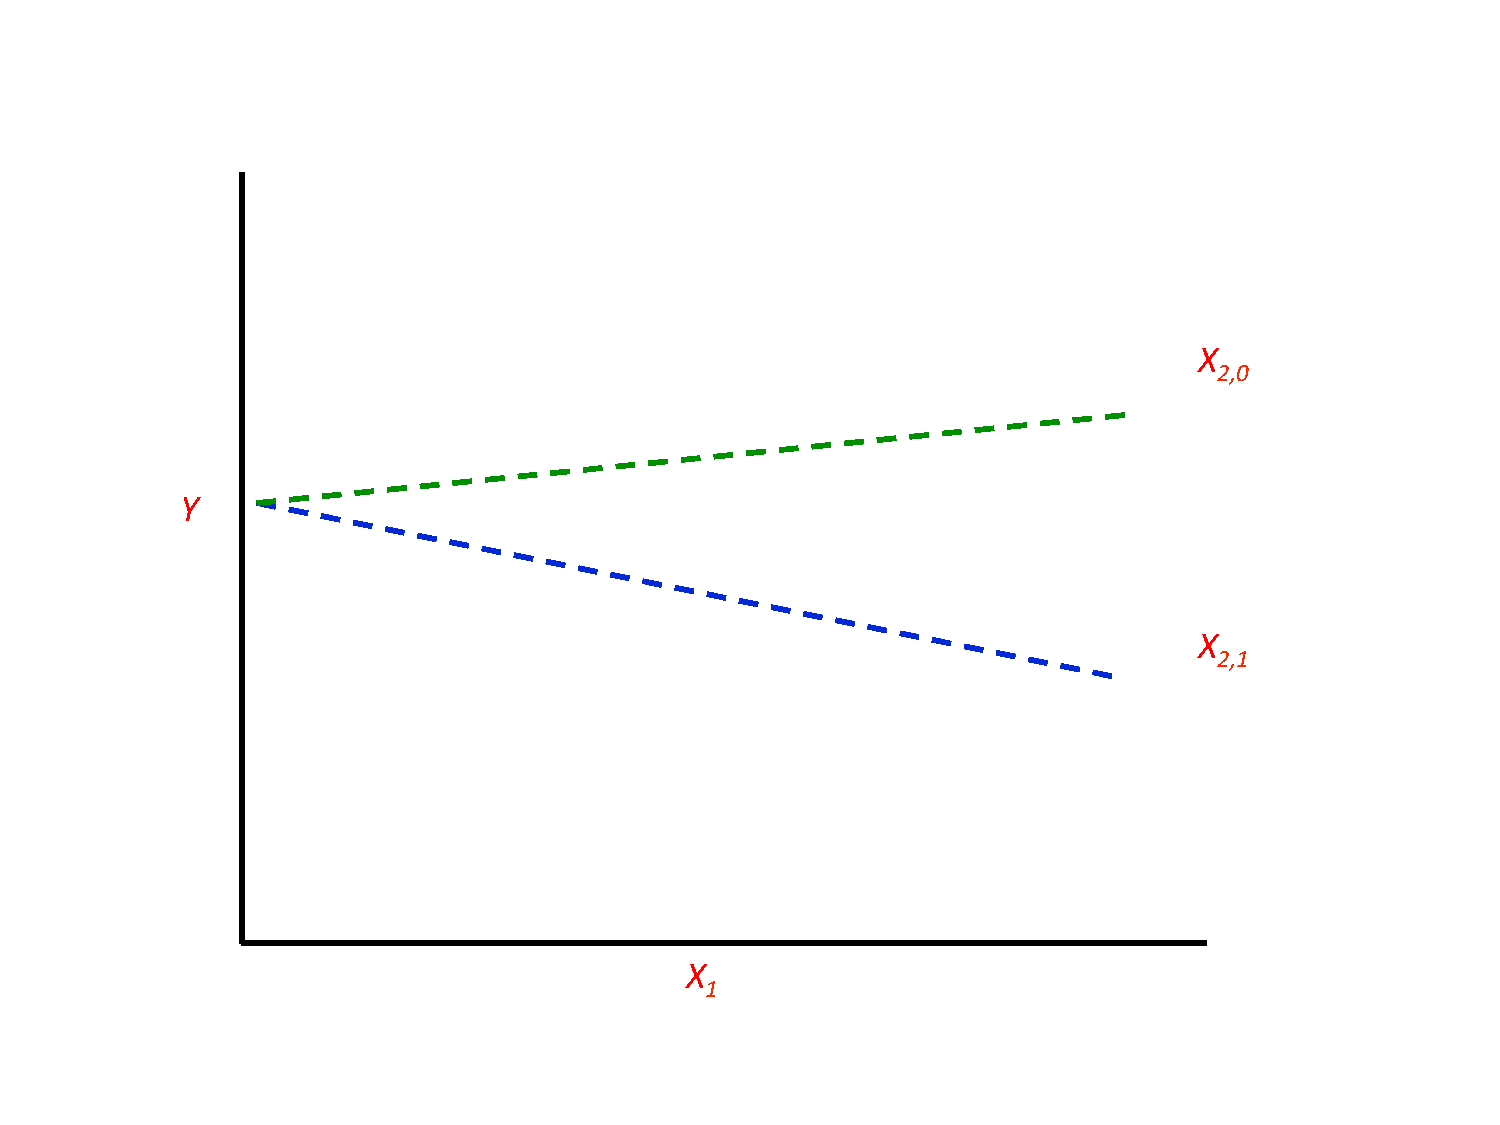
\includegraphics[width=5in]{14_Topics/duminter.pdf}
  \caption {Illustration of Slope Interaction \label{fig:dumin}}
\end{figure}

We can test our hypothesized interaction in \texttt{R}, controlling for the effects of age
and income. 
\begin{knitrout}
\definecolor{shadecolor}{rgb}{0.969, 0.969, 0.969}\color{fgcolor}\begin{kframe}
\begin{alltt}
\hlstd{ols2} \hlkwb{<-} \hlkwd{lm}\hlstd{(glbcc_risk} \hlopt{~} \hlstd{age} \hlopt{+} \hlstd{income} \hlopt{+} \hlstd{education} \hlopt{+} \hlstd{gender} \hlopt{*} \hlstd{ideol,}
    \hlkwc{data} \hlstd{= ds.temp)}
\hlkwd{summary}\hlstd{(ols2)}
\end{alltt}
\begin{verbatim}
## 
## Call:
## lm(formula = glbcc_risk ~ age + income + education + gender * 
##     ideol, data = ds.temp)
## 
## Residuals:
##    Min     1Q Median     3Q    Max 
## -8.718 -1.704  0.166  1.468  6.929 
## 
## Coefficients:
##                   Estimate    Std. Error t value             Pr(>|t|)    
## (Intercept)  10.6004885194  0.3296900513  32.153 < 0.0000000000000002 ***
## age          -0.0041366805  0.0036653120  -1.129              0.25919    
## income       -0.0000023222  0.0000009069  -2.561              0.01051 *  
## education     0.0682885587  0.0299249903   2.282              0.02258 *  
## gender        0.5971981026  0.2987398877   1.999              0.04572 *  
## ideol        -0.9591306050  0.0389448341 -24.628 < 0.0000000000000002 ***
## gender:ideol -0.1750006234  0.0597401590  -2.929              0.00343 ** 
## ---
## Signif. codes:  0 '***' 0.001 '**' 0.01 '*' 0.05 '.' 0.1 ' ' 1
## 
## Residual standard error: 2.427 on 2264 degrees of freedom
## Multiple R-squared:  0.3664,	Adjusted R-squared:  0.3647 
## F-statistic: 218.2 on 6 and 2264 DF,  p-value: < 0.00000000000000022
\end{verbatim}
\end{kframe}
\end{knitrout}
The results indicate a negative and significant interaction effect for gender and ideology. Consistent with our hypothesis, this means that the effect of ideology on climate change risk is more pronounced for males than females. Put differently, the slope of ideology is steeper for males than it is for females. This is shown in Figure \ref{fig:dummales}. 


\begin{figure}
  \centering
  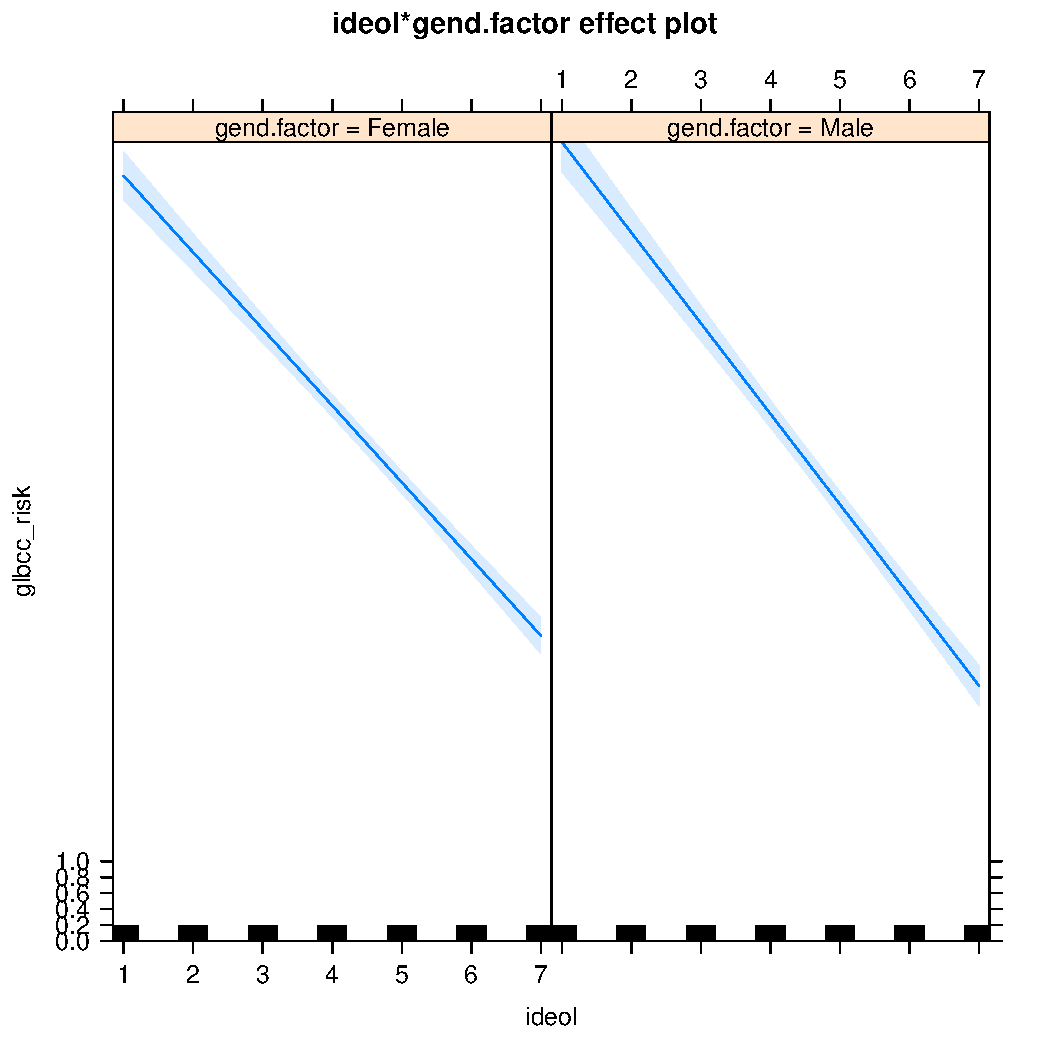
\includegraphics[width=4in]{14_Topics/dummales.pdf}%filename
  \caption {Interaction of Ideology and Gender \label{fig:dummales}}
\end{figure}

%above graphic had to remove ,length=5in

In sum, dummy variables add greatly to the flexibility of OLS model specification. They permit the inclusion of categorical variables, and they allow for testing hypotheses about interactions  of groups with other IVs within the model. This kind of flexibility is one reason that OLS models are widely used by social scientists and policy analysts.

\section{Standardized Regression Coefficients} 

In most cases, the various IVs in a model are represented on different measurement scales. For example, ideology ranges from 1 to 7, while age ranges from 18 to over 90 years old. These different scales make comparing the effects of the various IVs difficult.  If we want to directly compare the magnitudes of the effects of ideology and age on levels of environmental concern, we would need to \textbf{standardize} the variables. 

One way to standardized variables is to create a $Z$-score based on each variable. Variables are standardized in this way as follows:
\begin{equation}
  Z_i = \frac{X_i-\bar{X}}{s_x} 
\end{equation}
\noindent where $s_x$ is the s.d. of $X$. Standardizing the variables by creating $Z$-scores re-scales them so that each variables has a mean of $0$ and a s.d. of $1$. Therefore, all variables have same mean and s.d. It is important to realize (and it is somewhat counter-intuitive) that the standardized variables retain all of the variation that was in the original measure.

A second way to standardize variables converts the unstandardized $B$, into a standardized $B'$. 
\begin{equation}
  B'_k = B_k\frac{s_k}{s_Y}  
\end{equation}
where $B_k$ is the unstandardized coefficient of $X_k$, $s_k$ is the s.d. of $X_k$, and $s_y$ is the s.d. of $Y$. Standardized regression coefficients, also known as beta weights or ``betas", are those we would get if we regress a standardized $Y$ onto standardized $X$’s. 
 
\begin{grbox}
\greybox{\textbf{Interpreting Standardized Betas}

\begin{itemize}  
\item The standard deviation change in $Y$ for a one-standard deviation change in $X$ 
\item All $X$’s on a equal footing, so can compare the strength of the effects of the $X$’s 
\end{itemize}  

\textbf{Cannot be used for comparisons across samples}
\begin{itemize}
\item Variances will differ across different samples
\end{itemize}}
\end{grbox}

We can use the \texttt{scale} function in \texttt{R} to calculate a $Z$ score for each of our variables, and then re-run our model. 
\begin{knitrout}
\definecolor{shadecolor}{rgb}{0.969, 0.969, 0.969}\color{fgcolor}\begin{kframe}
\begin{alltt}
\hlstd{stan.ds} \hlkwb{<-} \hlstd{ds.temp} \hlopt \hlkwd{select}\hlstd{(glbcc_risk, age, education, income,}
    \hlstd{ideol, gender)} \hlopt \hlstd{scale} \hlopt \hlkwd{data.frame}\hlstd{()}

\hlstd{ols3} \hlkwb{<-} \hlkwd{lm}\hlstd{(glbcc_risk} \hlopt{~} \hlstd{age} \hlopt{+} \hlstd{education} \hlopt{+} \hlstd{income} \hlopt{+} \hlstd{ideol} \hlopt{+} \hlstd{gender,}
    \hlkwc{data} \hlstd{= stan.ds)}
\hlkwd{summary}\hlstd{(ols3)}
\end{alltt}
\begin{verbatim}
## 
## Call:
## lm(formula = glbcc_risk ~ age + education + income + ideol + 
##     gender, data = stan.ds)
## 
## Residuals:
##      Min       1Q   Median       3Q      Max 
## -2.92180 -0.54357  0.06509  0.48646  2.20164 
## 
## Coefficients:
##                           Estimate             Std. Error t value
## (Intercept)  0.0000000000000001685  0.0167531785616065292   0.000
## age         -0.0187675384877126518  0.0169621356203379960  -1.106
## education    0.0395657731919867237  0.0178239180606745221   2.220
## income      -0.0466922668201090602  0.0178816880127353542  -2.611
## ideol       -0.5882792369403809785  0.0170882328807871603 -34.426
## gender      -0.0359158695199312886  0.0170016561132237121  -2.112
##                         Pr(>|t|)    
## (Intercept)              1.00000    
## age                      0.26865    
## education                0.02653 *  
## income                   0.00908 ** 
## ideol       < 0.0000000000000002 ***
## gender                   0.03475 *  
## ---
## Signif. codes:  0 '***' 0.001 '**' 0.01 '*' 0.05 '.' 0.1 ' ' 1
## 
## Residual standard error: 0.7984 on 2265 degrees of freedom
## Multiple R-squared:  0.364,	Adjusted R-squared:  0.3626 
## F-statistic: 259.3 on 5 and 2265 DF,  p-value: < 0.00000000000000022
\end{verbatim}
\end{kframe}
\end{knitrout}

In addition, we can convert the original unstandardized coefficient for ideology, to a standardized coefficient. 
\begin{knitrout}
\definecolor{shadecolor}{rgb}{0.969, 0.969, 0.969}\color{fgcolor}\begin{kframe}
\begin{alltt}
\hlstd{sdX} \hlkwb{<-} \hlkwd{sd}\hlstd{(ds.temp}\hlopt{$}\hlstd{ideol,} \hlkwc{na.rm} \hlstd{=} \hlnum{TRUE}\hlstd{)}
\hlstd{sdY} \hlkwb{<-} \hlkwd{sd}\hlstd{(ds.temp}\hlopt{$}\hlstd{glbcc_risk,} \hlkwc{na.rm} \hlstd{=} \hlnum{TRUE}\hlstd{)}
\hlstd{ideology.prime} \hlkwb{<-} \hlstd{ols1}\hlopt{$}\hlstd{coef[}\hlnum{5}\hlstd{]} \hlopt{*} \hlstd{(sdX}\hlopt{/}\hlstd{sdY)}
\hlstd{ideology.prime}
\end{alltt}
\begin{verbatim}
##      ideol 
## -0.5882792
\end{verbatim}
\end{kframe}
\end{knitrout}

Using either approach, standardized coefficients allow us to compare the magnitudes of the effects of each of the IVs on $Y$.

\section{Summary}
This chapter has focused on options in designing and using OLS models. We first covered the use of dummy variables to capture the effects of group differences on estimates of $Y$. We then explained how dummy variables, when interacted with scale variables, can provide estimates of the differences in how the scale variable affects $Y$ across the different subgroups represented by the dummy variable. Finally, we introduced the use of standardized regression coefficients as a means to compare the effects of different $Xs$ on $Y$ when the scales of the $Xs$ differ. Overall, these refinements in the use of OLS permit great flexibility in the application of regression models to estimation and hypothesis testing in policy analysis and social science research.








\chapter{The Art of Regression Diagnostics} 

The previous chapters have focused on the mathematical bases of multiple OLS regression, the use of partial regression coefficients, and aspects of model design and construction. This chapter returns our focus to the assessment of the statistical adequacy of our models, first by revisiting the key assumptions necessary for OLS to provide the best, linear, unbiased estimates (BLUE) of the relationships between our model $Xs$ and $Y$. We will then discuss the ``art" of diagnosing the results of OLS for potential violations of the key OLS assumptions.  We refer to this diagnostic process as an art because there is no ``cook book approach" that defines precisely what to do when problems are detected. Note that the examples in this chapter use a subset dataset. This is a smaller data set, $n=500$, based on the first 500 observations of the full data set used in prior chapters. We use this smaller dataset in order to be able to illustrate, graphically, the diagnostic results described in this chapter.

\begin{knitrout}
\definecolor{shadecolor}{rgb}{0.969, 0.969, 0.969}\color{fgcolor}\begin{kframe}
\begin{alltt}
\hlcom{# create a new data frame with the first 500 observations}
\hlstd{ds.small} \hlkwb{<-} \hlkwd{filter}\hlstd{(ds)} \hlopt \hlkwd{select}\hlstd{(}\hlstr{"glbcc_risk"}\hlstd{,} \hlstr{"age"}\hlstd{,} \hlstr{"education"}\hlstd{,}
    \hlstr{"income"}\hlstd{,} \hlstr{"ideol"}\hlstd{)} \hlopt \hlkwd{slice}\hlstd{(}\hlnum{1}\hlopt{:}\hlnum{500}\hlstd{)} \hlopt \hlkwd{na.omit}\hlstd{()}

\hlcom{# For reference and experimentation here is code to randomly}
\hlcom{# draw 500 observations from the subset.  tbur.data.small <-}
\hlcom{# tbur.data[sample(1:nrow(tbur.data), 500, replace=FALSE),]}
\end{alltt}
\end{kframe}
\end{knitrout}

\section{OLS Error Assumptions Revisited} 

As described in earlier chapters, there is a set of key assumptions that must be met to justify the use of the $t$ and $F$ distributions in the interpretation of OLS model results. In particular, these assumptions are necessary for hypotheses tests and the generation of confidence intervals. When met, the assumptions make OLS more efficient than any other unbiased estimator. 

\begin{grbox}
 \greybox{\textbf{OLS Assumptions}
   
 \textit{Systematic Component}  
   \begin{itemize}
  \item Linearity 
  \item Fixed $X$  
  \end{itemize}

\textit{Stochastic Component}
 \begin{itemize}
 \item Errors have constant variance across the range of $X$
   \begin{center}
     $E(\epsilon^2_i) = \sigma^2_\epsilon$
   \end{center}
 \item Errors are independent of $X$ and other $\epsilon_i$
   \begin{center}
     $E(\epsilon_i) \equiv E(\epsilon|x_i) = 0$ 
     
     and 
     
     $E(\epsilon_i) \neq E(\epsilon_j)$ for $i \neq j$ 
   \end{center}
 \item Errors are normally distributed 
   \begin{center}
     $\epsilon_i \sim N(0,\sigma^2_\epsilon)$
   \end{center}
 \end{itemize}}
\end{grbox}
  

There is an additional set of assumptions needed for ``correct" model specification. A ideal model OLS would have the following characteristics: 
\begin{itemize}
\item $Y$ is a linear function of modeled $X$ variables
\item No $X$'s are omitted that affect $E(Y)$ and that are correlated with included $X$'s. Note that exclusion of other $X$s that are related to $Y$, but are not related to the $X$s in the model, does not critically undermine the model estimates. However, it does reduce the overall ability to explain $Y$. 
\item All $X$'s in the model affect $E(Y)$.  
\end{itemize}
Note that if we omit an $X$ that is related to $Y$ and other $X$s in the model, we will bias the estimate of the included $X$s.  Also consider the problem of including $X$s that are related to other $X$s in the model, but not related  to $Y$. This scenario would reduce the independent variance in $X$ used to predict $Y$.

Table \ref{tab:ass} summarizes the various classes of assumption failures and their implications. 

\begin{center}
\begin{table}[h]
\caption{Summary of OLS Assumption Failures and their Implications}
\label{tab:ass}
\begin{tabular}{lcccc}
\hline
Problem               & Biased $B$ & Biased $SE$ & Invalid $t$/$F$ & Hi Var \\
\hline
Non-linear            & Yes        & Yes         & Yes             & ---    \\
Heteroscedasticity    & No         & Yes         & Yes             & Yes    \\
Autocorrealtion       & No         & Yes         & Yes             & Yes    \\
Non-normal error      & No         & No          & Yes             & Yes    \\
Multicollinearity     & No         & No          & No              & Yes    \\
Omit relevant $X$     & Yes        & Yes         & Yes             & ---    \\
Irrelevant $X$        & No         & No          & No              & Yes    \\
$X$ measurement Error & Yes        & Yes         & Yes             & ---   \\
\hline
\end{tabular}
\end{table}
\end{center}

When considering the assumptions, our data permit empirical tests for some assumptions, but not all. Specifically, we can check for linearity, normality of the residuals, homoscedasticity, data ``outliers" and multicollinearity. However, we can't check for correlation between error and $X$'s, whether the mean error equals zero, and whether all the relevant $X$'s  are included. 

\section{OLS Diagnostic Techniques}

In this section, we examine the residuals from a multiple regression model for potential problems. Note that we use a subsample of the first 500 observations, drawn from the larger ``tbur.data" dataset, to permit easier evaluation of the plots of residuals. We begin with an evaluation of the assumption of the linearity of the relationship between the $X$s and $Y$, and then evaluate assumptions regarding the error term. 

Our multiple regression model predicts survey respondents' levels of risk perceived of climate change ($Y$) using political ideology, age, household income,  and educational achievement as independent variables ($X$s). The results of the regression model as follows:

\begin{knitrout}
\definecolor{shadecolor}{rgb}{0.969, 0.969, 0.969}\color{fgcolor}\begin{kframe}
\begin{alltt}
\hlstd{ols1} \hlkwb{<-} \hlkwd{lm}\hlstd{(glbcc_risk} \hlopt{~} \hlstd{age} \hlopt{+} \hlstd{education} \hlopt{+} \hlstd{income} \hlopt{+} \hlstd{ideol,} \hlkwc{data} \hlstd{= ds.small)}
\hlkwd{summary}\hlstd{(ols1)}
\end{alltt}
\begin{verbatim}
## 
## Call:
## lm(formula = glbcc_risk ~ age + education + income + ideol, data = ds.small)
## 
## Residuals:
##     Min      1Q  Median      3Q     Max 
## -7.1617 -1.7131 -0.0584  1.7216  6.8981 
## 
## Coefficients:
##                  Estimate    Std. Error t value            Pr(>|t|)    
## (Intercept) 12.0848259959  0.7246993630  16.676 <0.0000000000000002 ***
## age         -0.0055585796  0.0084072695  -0.661               0.509    
## education   -0.0186146680  0.0697901408  -0.267               0.790    
## income       0.0000001923  0.0000022269   0.086               0.931    
## ideol       -1.2235648372  0.0663035792 -18.454 <0.0000000000000002 ***
## ---
## Signif. codes:  0 '***' 0.001 '**' 0.01 '*' 0.05 '.' 0.1 ' ' 1
## 
## Residual standard error: 2.353 on 445 degrees of freedom
## Multiple R-squared:  0.4365,	Adjusted R-squared:  0.4315 
## F-statistic: 86.19 on 4 and 445 DF,  p-value: < 0.00000000000000022
\end{verbatim}
\end{kframe}
\end{knitrout}

On the basis of the $R$ output, the model appears to be quite reasonable, with a statistically significant estimated partial regression coefficient for political ideology. But let's take a closer look.

\subsection{Non-Linearity} 

One of the most critical assumptions of OLS is that the relationships between variables are linear in their functional form. We start with a stylized example (a fancy way of saying we made it up!) of what a linear and nonlinear pattern of residuals would look like. Figure \ref{fig:convar2} shows an illustration of how the residuals would look with a clearly linear relationship, and Figure \ref{fig:nonlin} illustrates how the the residuals would look with a clearly non-linear relationship.  





\begin{figure}
        \centering
        \begin{subfigure}[b]{0.45\textwidth}
                \centering
                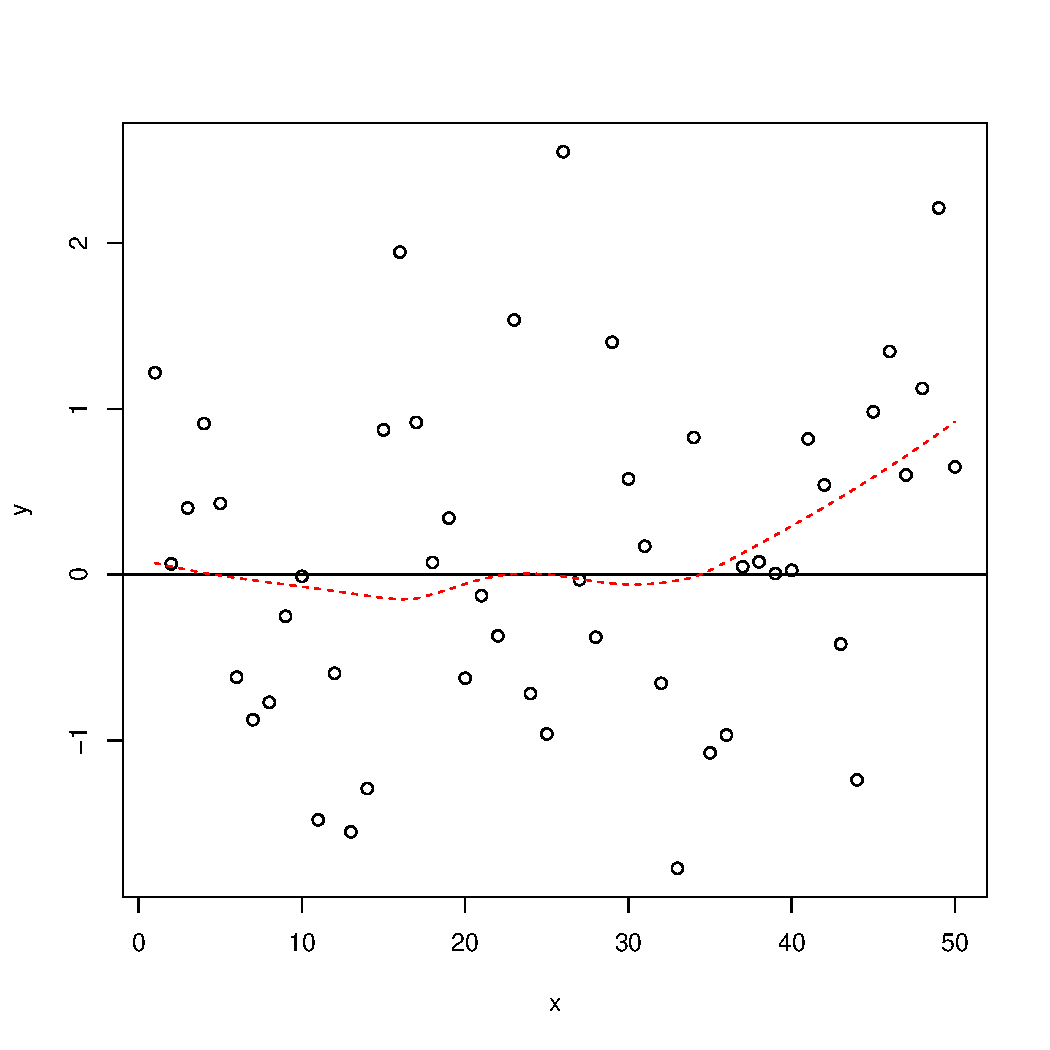
\includegraphics[width=\textwidth]{15_Diagnostics/convar2.pdf}%filename
                \caption{Linear \label{fig:convar2}}
        \end{subfigure}
        \begin{subfigure}[b]{0.45\textwidth}
                \centering
                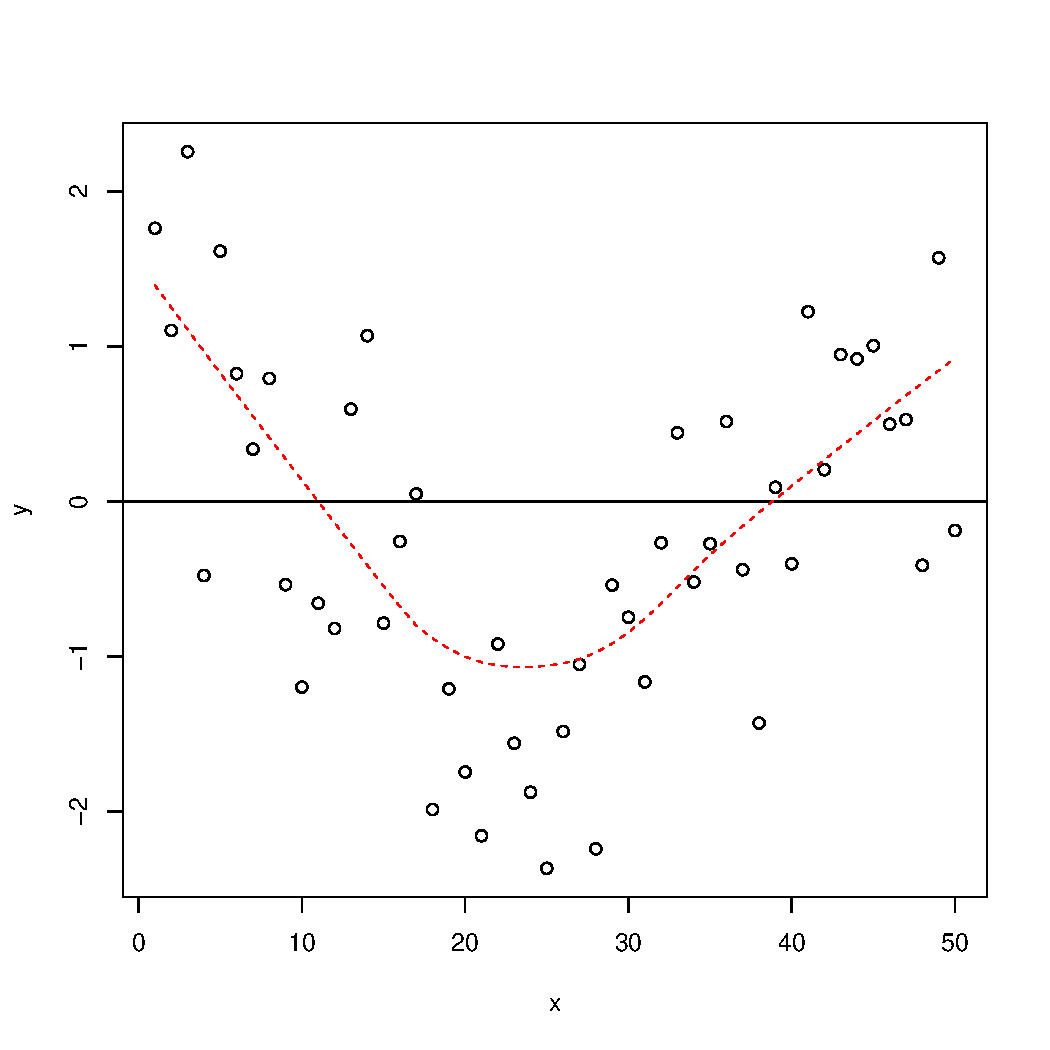
\includegraphics[width=\textwidth]{15_Diagnostics/nonlin.pdf}
                \caption{Non-Linear \label{fig:nonlin}}
        \end{subfigure}
        \caption{Made Up Residual Examples}
\end{figure} 

Now let's look at the residuals from our example model. We can check the linear nature of the relationship between the DV and the IVs in several ways. First we can plot the residuals by the values of the IVs. We also can add a lowess line to demonstrate the relationship between each of the IVs and the residuals, and add a line at $0$ for comparison. 

\begin{knitrout}
\definecolor{shadecolor}{rgb}{0.969, 0.969, 0.969}\color{fgcolor}\begin{kframe}
\begin{alltt}
\hlstd{ds.small}\hlopt{$}\hlstd{fit.r} \hlkwb{<-} \hlstd{ols1}\hlopt{$}\hlstd{residuals}
\hlstd{ds.small}\hlopt{$}\hlstd{fit.p} \hlkwb{<-} \hlstd{ols1}\hlopt{$}\hlstd{fitted.values}
\end{alltt}
\end{kframe}
\end{knitrout}


\begin{knitrout}
\definecolor{shadecolor}{rgb}{0.969, 0.969, 0.969}\color{fgcolor}\begin{kframe}
\begin{alltt}
\hlstd{ds.small} \hlopt \hlkwd{melt}\hlstd{(}\hlkwc{measure.vars} \hlstd{=} \hlkwd{c}\hlstd{(}\hlstr{"age"}\hlstd{,} \hlstr{"education"}\hlstd{,} \hlstr{"income"}\hlstd{,}
    \hlstr{"ideol"}\hlstd{,} \hlstr{"fit.p"}\hlstd{))} \hlopt \hlkwd{ggplot}\hlstd{(}\hlkwd{aes}\hlstd{(value, fit.r,} \hlkwc{group} \hlstd{= variable))} \hlopt{+}
    \hlkwd{geom_point}\hlstd{(}\hlkwc{shape} \hlstd{=} \hlnum{1}\hlstd{)} \hlopt{+} \hlkwd{geom_smooth}\hlstd{(}\hlkwc{method} \hlstd{= loess)} \hlopt{+} \hlkwd{geom_hline}\hlstd{(}\hlkwc{yintercept} \hlstd{=} \hlnum{0}\hlstd{)} \hlopt{+}
    \hlkwd{facet_wrap}\hlstd{(}\hlopt{~}\hlstd{variable,} \hlkwc{scales} \hlstd{=} \hlstr{"free"}\hlstd{)}
\hlkwd{dev.off}\hlstd{()}
\end{alltt}
\end{kframe}
\end{knitrout}
\begin{figure}
        \centering
        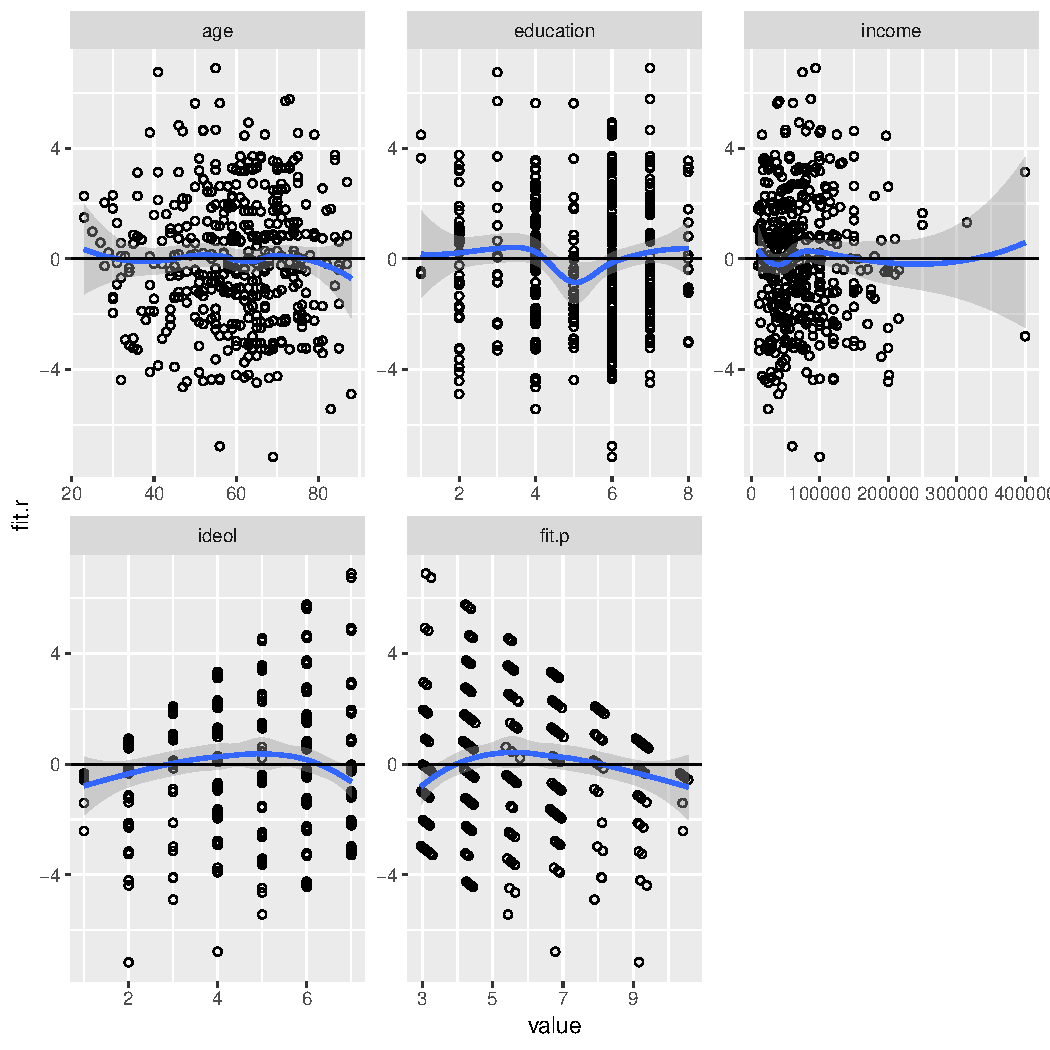
\includegraphics[width=4in]{15_Diagnostics/multlin.pdf}%filename
        \caption{Checking for Non-Linearity \label{fig:multlin}}
\end{figure}        

\noindent As we can see in Figure \ref{fig:multlin}, the plots of residuals by both income and ideology seem to indicate non-linear relationships. We can check this ``ocular impression" by squaring each term and using the \texttt{anova} function to compare model fit.
\begin{knitrout}
\definecolor{shadecolor}{rgb}{0.969, 0.969, 0.969}\color{fgcolor}\begin{kframe}
\begin{alltt}
\hlstd{ds.small}\hlopt{$}\hlstd{age2} \hlkwb{<-} \hlstd{ds.small}\hlopt{$}\hlstd{age}\hlopt{^}\hlnum{2}
\hlstd{ds.small}\hlopt{$}\hlstd{edu2} \hlkwb{<-} \hlstd{ds.small}\hlopt{$}\hlstd{education}\hlopt{^}\hlnum{2}
\hlstd{ds.small}\hlopt{$}\hlstd{inc2} \hlkwb{<-} \hlstd{ds.small}\hlopt{$}\hlstd{income}\hlopt{^}\hlnum{2}
\hlstd{ds.small}\hlopt{$}\hlstd{ideology2} \hlkwb{<-} \hlstd{ds.small}\hlopt{$}\hlstd{ideol}\hlopt{^}\hlnum{2}
\hlstd{ols2} \hlkwb{<-} \hlkwd{lm}\hlstd{(glbcc_risk} \hlopt{~} \hlstd{age} \hlopt{+} \hlstd{age2} \hlopt{+} \hlstd{education} \hlopt{+} \hlstd{edu2} \hlopt{+} \hlstd{income} \hlopt{+}
    \hlstd{inc2} \hlopt{+} \hlstd{ideol} \hlopt{+} \hlstd{ideology2,} \hlkwc{data} \hlstd{= ds.small)}
\hlkwd{summary}\hlstd{(ols2)}
\end{alltt}
\begin{verbatim}
## 
## Call:
## lm(formula = glbcc_risk ~ age + age2 + education + edu2 + income + 
##     inc2 + ideol + ideology2, data = ds.small)
## 
## Residuals:
##     Min      1Q  Median      3Q     Max 
## -7.1563 -1.5894  0.0389  1.4898  7.3417 
## 
## Coefficients:
##                      Estimate        Std. Error t value    Pr(>|t|)    
## (Intercept)  9.66069872535646  1.93057305147186   5.004 0.000000812 ***
## age          0.02973349791714  0.05734762412523   0.518    0.604385    
## age2        -0.00028910659305  0.00050097599702  -0.577    0.564175    
## education   -0.48137978481400  0.35887879735475  -1.341    0.180499    
## edu2         0.05131569933892  0.03722361864679   1.379    0.168723    
## income       0.00000285263412  0.00000534134363   0.534    0.593564    
## inc2        -0.00000000001131  0.00000000001839  -0.615    0.538966    
## ideol       -0.05726196851107  0.35319018414228  -0.162    0.871279    
## ideology2   -0.13270718319750  0.03964680646295  -3.347    0.000886 ***
## ---
## Signif. codes:  0 '***' 0.001 '**' 0.01 '*' 0.05 '.' 0.1 ' ' 1
## 
## Residual standard error: 2.33 on 441 degrees of freedom
## Multiple R-squared:  0.4528,	Adjusted R-squared:  0.4429 
## F-statistic: 45.61 on 8 and 441 DF,  p-value: < 0.00000000000000022
\end{verbatim}
\end{kframe}
\end{knitrout}

\noindent The model output indicates that ideology may have a non-linear relationships with risk perceptions of climate change.     For ideology, only the squared term is significant, indicating that levels of perceived risk of climate change decline at an increasing rate for those on the most conservative end of the scale.  Again, this is consistent with the visual inspection of the relationship between ideology and the residuals in Figure \ref{fig:multlin}.   The question remains whether the introduction of these non-linear (polynomial) terms improves overall model fit.  We can check that with an analysis of variance across the simple model (without polynomial terms) and the models with the squared terms.

\begin{knitrout}
\definecolor{shadecolor}{rgb}{0.969, 0.969, 0.969}\color{fgcolor}\begin{kframe}
\begin{alltt}
\hlkwd{anova}\hlstd{(ols1, ols2)}
\end{alltt}
\begin{verbatim}
## Analysis of Variance Table
## 
## Model 1: glbcc_risk ~ age + education + income + ideol
## Model 2: glbcc_risk ~ age + age2 + education + edu2 + income + inc2 + 
##     ideol + ideology2
##   Res.Df    RSS Df Sum of Sq      F  Pr(>F)  
## 1    445 2464.2                              
## 2    441 2393.2  4    71.059 3.2736 0.01161 *
## ---
## Signif. codes:  0 '***' 0.001 '**' 0.01 '*' 0.05 '.' 0.1 ' ' 1
\end{verbatim}
\end{kframe}
\end{knitrout}


\noindent As we can see, the Anova test indicates that including the squared terms improves model fit, therefore the relationships include nonlinear components. 

A final way to check for non-linearity is Ramsey's Regression Error Specification Test (RESET). This tests the functional form of the model. Similar to our test using squared terms, the RESET tests calculates an $F$ statistic that compares the linear model with a model(s) that raises the IVs to various powers. Specifically, it tests whether there are statistically significant differences in the $R^2$ of each of the models. Similar to a nested $F$ test, it is calculated by: 

\begin{equation}
  \label{eq:reset}
  F = \frac{\frac{R^2_1-R^2_0}{q}}{\frac{1-R^2_1}{n-k_1}}
\end{equation}

\noindent where $R^2_0$ is the $R^2$ of the linear model, $R^2_1$ is the $R^2$ of the polynomial model(s), $q$ is the number of new regressors, and $k_1$ is the number of IVs in the polynomial model(s). The null hypothesis is that the functional relationship between the $X$'s and $Y$ is linear, therefore the coefficients of the second and third powers to the IVs are zero.  If there is a low $p$-value (i.e., if we can reject the null hypothesis), non-linear relationships are suspected.  This test can be run using the \texttt{resettest} function from the \texttt{lmtest} package. Here we are setting the IVs to the second and third powers and we are examining the regressor variables.\footnote{See the \texttt{lmtest} package documentation for more options and information.}   
  
\begin{knitrout}
\definecolor{shadecolor}{rgb}{0.969, 0.969, 0.969}\color{fgcolor}\begin{kframe}
\begin{alltt}
\hlkwd{library}\hlstd{(lmtest)}
\hlkwd{resettest}\hlstd{(ols1,} \hlkwc{power} \hlstd{=} \hlnum{2}\hlopt{:}\hlnum{3}\hlstd{,} \hlkwc{type} \hlstd{=} \hlstr{"regressor"}\hlstd{)}
\end{alltt}
\begin{verbatim}
## 
## 	RESET test
## 
## data:  ols1
## RESET = 2.2752, df1 = 8, df2 = 437, p-value = 0.02157
\end{verbatim}
\end{kframe}
\end{knitrout}

\noindent Again, the test provides evidence that we have a non-linear relationship. 

What should we do when we identify a nonlinear relationship between our $Y$ and $X$s ?  The first step is to look closely at the bi-variate plots, to try to discern the correct functional form for each $X$ regressor. If the relationship looks curvilinear, try a polynomial regression in which you include both $X$ and $X^2$ for the relevant IVs. It may also be the case that a skewed DV or IV is causing the problem. This is not unusual when, for example, the income variable plays an important role in the model, and the distribution of income is skewed upward. In such a case, you can try transforming the skewed variable, using an appropriate log form.

It is possible that variable transformations won't suffice, however. In that case, you may have no other option by to try non-linear forms of regression. These non-OLS kinds of models typically use maximal likelihood functions (see the next chapter) to fit the model to the data. But  that takes us considerably beyond the focus of this book.

\subsection{Non-Constant Variance, or Heteroscedasticity}

Recall that OLS requires constant variance because the even spread of residuals is assumed for both $F$ and $t$ tests. To examine constant variance, we can produce (read as ``make up") a baseline plot to demonstrate what constant variance in the residuals ``should" look like. 

As we can see in Figure \ref{fig:convar15}, the residuals are spread evenly and in a seemingly random fashion, much like the ``sneeze plot" discussed in Chapter 10.  This is the ideal pattern, indicating that the residuals do not vary systematically over the range of the predicted value for $X$. The residuals are homoscedastistic, and thus provide the appropriate basis for the $F$ and $t$ tests needed for evaluating your hypotheses.

We can also present a clearly heteroscedastistic residual term. In this case the residuals do vary systematically over the range of $X$, indicating that the precision of the estimates of $Y$ will vary considerably over the range of predicted values. Note the distinctive fan shape in Figure \ref{fig:hetero15}, indicating that predictions of $Y$ lose precision as the value of $X$ increases. 



\begin{figure}
        \centering
        \begin{subfigure}[b]{0.45\textwidth}
                \centering
                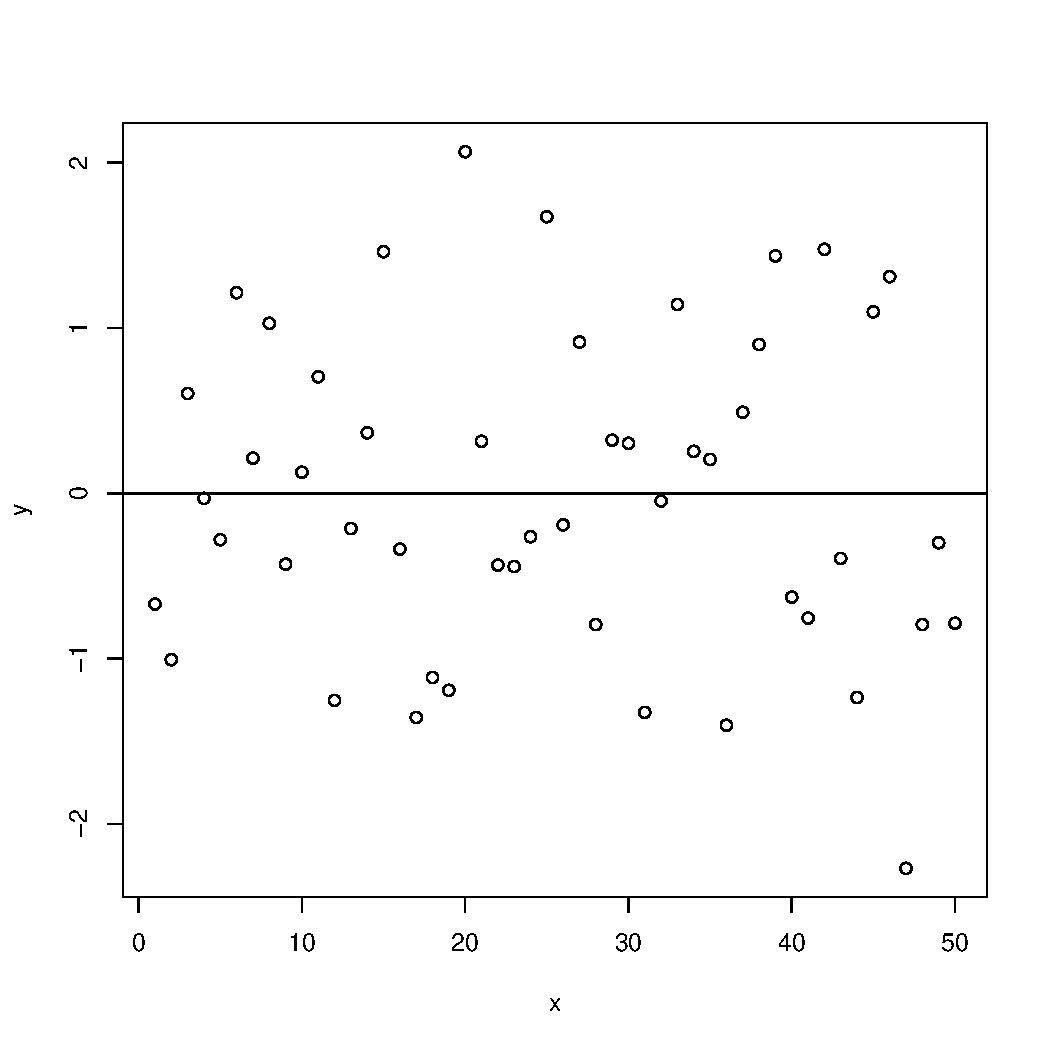
\includegraphics[width=\textwidth]{15_Diagnostics/convar.pdf}%filename
                \caption{Constant Variance \label{fig:convar15}}
        \end{subfigure}
        \begin{subfigure}[b]{0.45\textwidth}
                \centering
                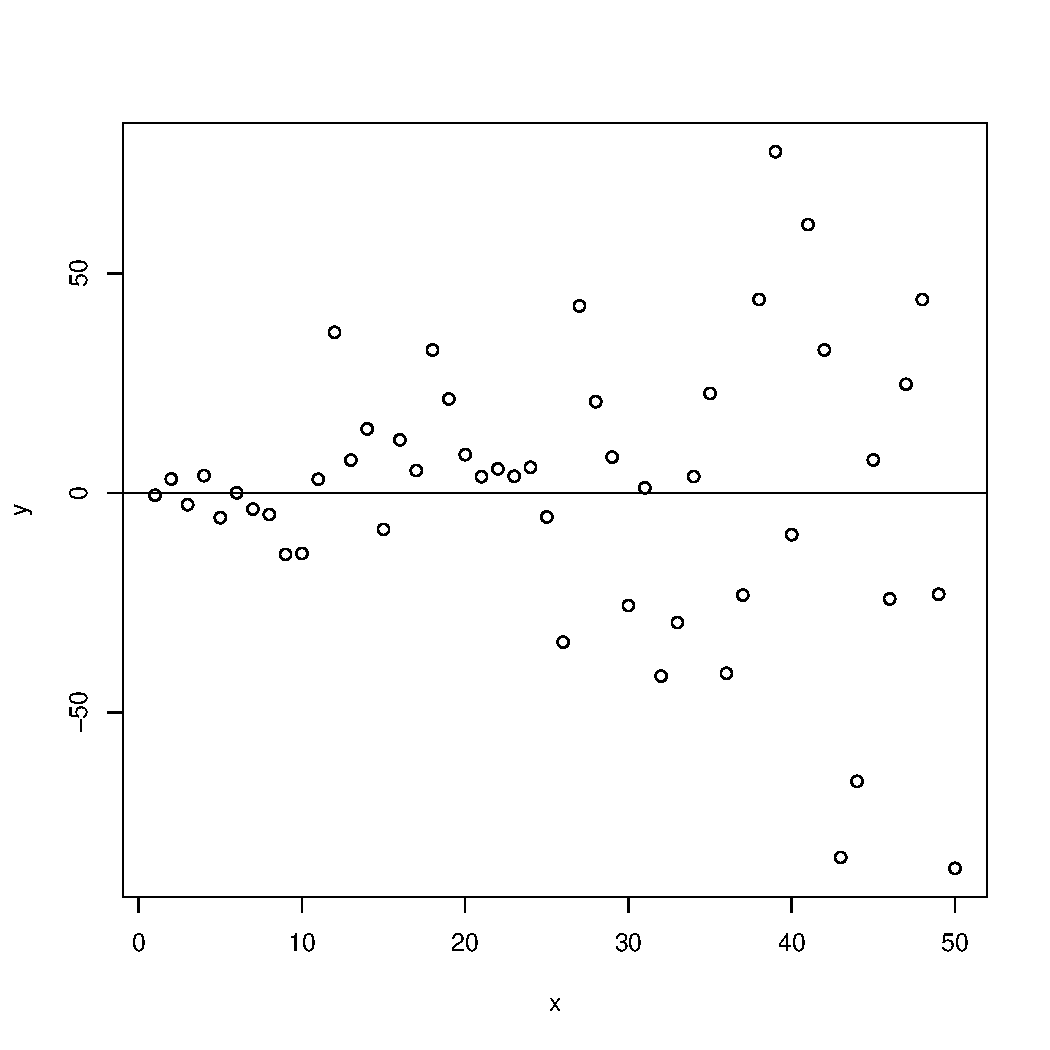
\includegraphics[width=\textwidth]{15_Diagnostics/heterovar.pdf}%filename
                \caption{Heteroscedasticity \label{fig:hetero15}}
        \end{subfigure}
        \caption{Made Up Residual Examples}
\end{figure}  

The first step in determining whether we have constant variance is to plot the the residuals by the fitted values for $Y$, as follows:\footnote{Note that we jitter the points to make them easier to see.}

\begin{knitrout}
\definecolor{shadecolor}{rgb}{0.969, 0.969, 0.969}\color{fgcolor}\begin{kframe}
\begin{alltt}
\hlstd{ds.small}\hlopt{$}\hlstd{fit.r} \hlkwb{<-} \hlstd{ols1}\hlopt{$}\hlstd{residuals}
\hlstd{ds.small}\hlopt{$}\hlstd{fit.p} \hlkwb{<-} \hlstd{ols1}\hlopt{$}\hlstd{fitted.values}
\end{alltt}
\end{kframe}
\end{knitrout}

\begin{figure}
        \centering
        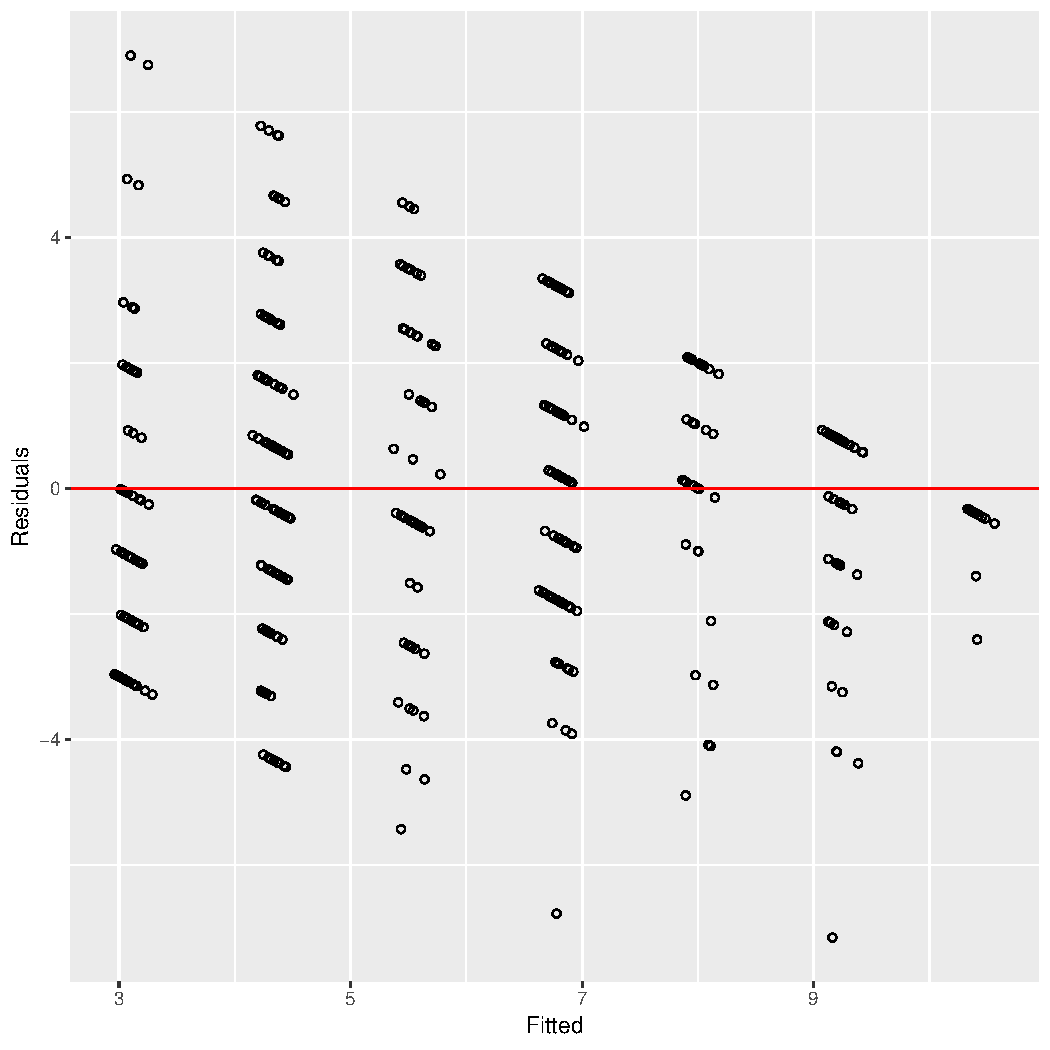
\includegraphics[width=4in]{15_Diagnostics/multregres.pdf}%filename
        \caption{Multiple Regression Residuals and Fitted Values \label{fig:multregres}}
\end{figure}

\noindent Based on the pattern evident in Figure \ref{fig:multregres}, the residuals
appear to show heteroscedasticity. We can test for non-constant error using the Breusch-Pagan (aka Cook-Weisberg) test. This tests the null hypothesis that the error variance is constant, therefore a small p value would indicate that we have heteroscedasticity. In R we can use the ncvTest function from the car package.

\begin{knitrout}
\definecolor{shadecolor}{rgb}{0.969, 0.969, 0.969}\color{fgcolor}\begin{kframe}
\begin{alltt}
\hlkwd{library}\hlstd{(car)}
\hlkwd{ncvTest}\hlstd{(ols1)}
\end{alltt}
\begin{verbatim}
## Non-constant Variance Score Test 
## Variance formula: ~ fitted.values 
## Chisquare = 12.70938, Df = 1, p = 0.00036383
\end{verbatim}
\end{kframe}
\end{knitrout}
\noindent The non-constant variance test provides confirmation that the residuals from our model are heteroscedastistic.

What are the implications? Our $t$-tests for the estimated partial regression  coefficients assumed constant variance. With the evidence of heteroscedasticity, we conclude that these tests are unreliable (the precision of our estimates will be greater in some ranges of $X$ than others). 

They are several steps that can be considered when confronted by heteroscedasticity in the residuals. First, we can consider whether we need to re-specify the model, possibly because we have some omitted variables. If model re-specification does not correct the problem, we can use non-OLS regression techniques that include robust estimated  standard errors.  Robust standard errors are appropriate when error variance is unknown. Robust standard errors do not change the estimate of $B$, but adjust the estimated standard error of each coefficient, $SE(B)$, thus giving more accurate $p$ values. In this example, we draw on White's (1980)\footnote{H White,  1980.  ``A Heteroskedasticity-consistent covariance matrix estimator and a direct test for heteroskedasticity." \underline{Econometrica} 48: 817-838.} method to calculate robust standard errors.  

White uses a \textbf{heteroskedasticity consistent covariance matrix} (hccm) to calculate standard errors when the error term has non-constant variance. Under the OLS assumption of constant error variance, the covariance matrix of $b$ is:
\begin{equation*}
  V(b) = (X'X)^{-1} X'V(y)X(X'X)^{-1}
\end{equation*}
\noindent where $V(y)=\sigma^{2}_{e}I_n$, therefore,
$V(b)=\sigma^{2}_{e}(X'X)^{-1}$. If the error terms have distinct
variances, a consistent estimator constrains $\Sigma$ to a diagonal
matrix of the squared residuals,
$\Sigma=\text{diag}(\sigma^2_1,\ldots,\sigma^2_n)$ where $\sigma^2_i$
is estimated by $e^2_i$. Therefore the hccm estimator is expressed as:  
\begin{equation*}
 V_{hccm}(b) = (X'X)^{-1} X'\text{diag}(e^2_i,\ldots,e^2_n) X(X'X)^{-1} 
\end{equation*}

We can use the \texttt{hccm} function from the \texttt{car} package to calculate the robust standard errors for our regression model, predicting perceived environmental risk ($Y$) with political ideology, age, education and income as the $X$ variables. 
\begin{knitrout}
\definecolor{shadecolor}{rgb}{0.969, 0.969, 0.969}\color{fgcolor}\begin{kframe}
\begin{alltt}
\hlkwd{library}\hlstd{(car)}
\hlkwd{hccm}\hlstd{(ols1)} \hlopt \hlkwd{diag}\hlstd{()} \hlopt \hlkwd{sqrt}\hlstd{()}
\end{alltt}
\begin{verbatim}
##    (Intercept)            age      education         income          ideol 
## 0.668778725013 0.008030365625 0.069824489564 0.000002320899 0.060039031426
\end{verbatim}
\end{kframe}
\end{knitrout}

Using the \texttt{hccm} function we can create a function in \texttt{R} that will calculate the robust standard errors and the subsequent $t$-values and $p$-values. 
\begin{knitrout}
\definecolor{shadecolor}{rgb}{0.969, 0.969, 0.969}\color{fgcolor}\begin{kframe}
\begin{alltt}
\hlkwd{library}\hlstd{(car)}
\hlstd{robust.se} \hlkwb{<-} \hlkwa{function}\hlstd{(}\hlkwc{model}\hlstd{) \{}
    \hlstd{s} \hlkwb{<-} \hlkwd{summary}\hlstd{(model)}
    \hlstd{wse} \hlkwb{<-} \hlkwd{sqrt}\hlstd{(}\hlkwd{diag}\hlstd{(}\hlkwd{hccm}\hlstd{(ols1)))}
    \hlstd{t} \hlkwb{<-} \hlstd{model}\hlopt{$}\hlstd{coefficients}\hlopt{/}\hlstd{wse}
    \hlstd{p} \hlkwb{<-} \hlnum{2} \hlopt{*} \hlkwd{pnorm}\hlstd{(}\hlopt{-}\hlkwd{abs}\hlstd{(t))}
    \hlstd{results} \hlkwb{<-} \hlkwd{cbind}\hlstd{(model}\hlopt{$}\hlstd{coefficients, wse, t, p)}
    \hlkwd{dimnames}\hlstd{(results)} \hlkwb{<-} \hlkwd{dimnames}\hlstd{(s}\hlopt{$}\hlstd{coefficients)}
    \hlstd{results}
\hlstd{\}}
\end{alltt}
\end{kframe}
\end{knitrout}

We can then compare our results with the original simple regression model results. 
\begin{knitrout}
\definecolor{shadecolor}{rgb}{0.969, 0.969, 0.969}\color{fgcolor}\begin{kframe}
\begin{alltt}
\hlkwd{summary}\hlstd{(ols1)}
\end{alltt}
\begin{verbatim}
## 
## Call:
## lm(formula = glbcc_risk ~ age + education + income + ideol, data = ds.small)
## 
## Residuals:
##     Min      1Q  Median      3Q     Max 
## -7.1617 -1.7131 -0.0584  1.7216  6.8981 
## 
## Coefficients:
##                  Estimate    Std. Error t value            Pr(>|t|)    
## (Intercept) 12.0848259959  0.7246993630  16.676 <0.0000000000000002 ***
## age         -0.0055585796  0.0084072695  -0.661               0.509    
## education   -0.0186146680  0.0697901408  -0.267               0.790    
## income       0.0000001923  0.0000022269   0.086               0.931    
## ideol       -1.2235648372  0.0663035792 -18.454 <0.0000000000000002 ***
## ---
## Signif. codes:  0 '***' 0.001 '**' 0.01 '*' 0.05 '.' 0.1 ' ' 1
## 
## Residual standard error: 2.353 on 445 degrees of freedom
## Multiple R-squared:  0.4365,	Adjusted R-squared:  0.4315 
## F-statistic: 86.19 on 4 and 445 DF,  p-value: < 0.00000000000000022
\end{verbatim}
\begin{alltt}
\hlkwd{robust.se}\hlstd{(ols1)}
\end{alltt}
\begin{verbatim}
##                     Estimate     Std. Error      t value
## (Intercept) 12.0848259958670 0.668778725013  18.06999168
## age         -0.0055585796372 0.008030365625  -0.69219509
## education   -0.0186146679570 0.069824489564  -0.26659225
## income       0.0000001922905 0.000002320899   0.08285175
## ideol       -1.2235648372311 0.060039031426 -20.37948994
##                                                                                                         Pr(>|t|)
## (Intercept) 0.00000000000000000000000000000000000000000000000000000000000000000000000054921988962793404323143119
## age         0.48881482326776815039437451559933833777904510498046875000000000000000000000000000000000000000000000
## education   0.78978312137982031870819810137618333101272583007812500000000000000000000000000000000000000000000000
## income      0.93396941638148500697269582815351895987987518310546875000000000000000000000000000000000000000000000
## ideol       0.00000000000000000000000000000000000000000000000000000000000000000000000000000000000000000002542911
\end{verbatim}
\end{kframe}
\end{knitrout}
\noindent As we see the estimated $B$'s remain the same, but the estimated standard errors, $t$-values and $p$-values are adjusted to reflect the robust estimation. Despite these adjustments, the results of the hypothesis test remain unchanged.

It is important to note that, while robust estimators can help atone for heteroscedasticity in your models, their use \texttt{should not} be seen as an alternative to careful model construction. The first step should always be to evaluate your model specification and functional form (e.g., the use of polynomials, inclusion of relevant variables), as well as possible measurement error, before resorting to robust estimation.

\subsection{Independence of $E$} 

As noted above, we cannot test for the assumption that the error term $E$ is independent of the $X$'s.  However we can test to see whether the error terms, $E_i$, are correlated with each other. One of the assumptions of OLS is that   $E(\epsilon_i) \neq E(\epsilon_j)$ for $i \neq j$. When there is a relationship between the residuals, this is referred to as serial correlation or \textbf{autocorrelation}. Autocorrelation is most likely to occur with time-series data, however it can occur with cross-sectional data as well. To test for autocorrelation we use the Durbin-Watson, $d$, test statistic. The $d$ statistic is expressed as:

\begin{equation}
  \label{eq:dw}
  d = \frac{\sum_{i=2}^{n} (E_i-E_{i-1})^{2}}{\sum_{i=1}^{n} E^{2}_i}
\end{equation}

The $d$ statistics ranges from $0$ to $4$; $0 \leq d \leq 4$. A  $0$ indicates perfect positive correction, $4$ indicates perfect negative correlation, and a $2$ indicates no autocorrelation. Therefore, we look for values of $d$ that are close to $2$.  

We can use the \texttt{dwtest} function in the \texttt{lmtest} package to test the null hypothesis that autocorrelation is $0$, meaning that we don't have autocorrelation. 

\begin{knitrout}
\definecolor{shadecolor}{rgb}{0.969, 0.969, 0.969}\color{fgcolor}\begin{kframe}
\begin{alltt}
\hlkwd{library}\hlstd{(lmtest)}
\hlkwd{dwtest}\hlstd{(ols1)}
\end{alltt}
\begin{verbatim}
## 
## 	Durbin-Watson test
## 
## data:  ols1
## DW = 1.9008, p-value = 0.1441
## alternative hypothesis: true autocorrelation is greater than 0
\end{verbatim}
\end{kframe}
\end{knitrout}
\noindent Generally, a Durbin-Watson result between 1.5 and 2.5 indicates, that any autocorrelation in the data will not have a discernible effect on your estimates.  The test for our example model indicates that we do not have an autocorrelation problem with this model. If we did find autocorrelation, we would need to respecify our model to account for (or estimate) the relationships among the error terms. In time series analysis, where observations are taken sequentially over time, we would typically include a ``lag" term (in which the value of $Y$ in period $t$ is predicted by the value of $Y$ in period $t-1$). This is a typical $AR1$ model, which would be discussed in a time-series analysis course. The entangled residuals  can, of course, be much more complex, and require more specialized models (e.g.,  ARIMA or vector-autoregression models). These approaches are beyond the  scope of this text.

\subsection{Normality of the Residuals} 

This is a critical assumption for OLS because (along with homoscedasticity) it is required for  hypothesis tests and confidence interval estimation. It is particularly sensitive with small samples. Note that non-normality will increase sample-to-sample variation in model estimates. 

To examine normality of the residuals we first plot the residuals and then run what is known as the Shapiro-Wilk normality test. Here we run the test on our example model, and plot the residuals.

\begin{knitrout}
\definecolor{shadecolor}{rgb}{0.969, 0.969, 0.969}\color{fgcolor}\begin{kframe}
\begin{alltt}
\hlkwd{ggplot}\hlstd{(ds.small,} \hlkwd{aes}\hlstd{(fit.r))} \hlopt{+} \hlkwd{geom_histogram}\hlstd{(}\hlkwc{bins} \hlstd{=} \hlnum{10}\hlstd{,} \hlkwc{color} \hlstd{=} \hlstr{"black"}\hlstd{,}
    \hlkwc{fill} \hlstd{=} \hlstr{"white"}\hlstd{)}
\end{alltt}
\end{kframe}
\end{knitrout}

\begin{knitrout}
\definecolor{shadecolor}{rgb}{0.969, 0.969, 0.969}\color{fgcolor}\begin{kframe}
\begin{alltt}
\hlkwd{ggplot}\hlstd{(ds.small,} \hlkwd{aes}\hlstd{(fit.r))} \hlopt{+} \hlkwd{geom_density}\hlstd{()} \hlopt{+} \hlkwd{stat_function}\hlstd{(}\hlkwc{fun} \hlstd{= dnorm,}
    \hlkwc{args} \hlstd{=} \hlkwd{list}\hlstd{(}\hlkwc{mean} \hlstd{=} \hlkwd{mean}\hlstd{(ds.small}\hlopt{$}\hlstd{fit.r),} \hlkwc{sd} \hlstd{=} \hlkwd{sd}\hlstd{(ds.small}\hlopt{$}\hlstd{fit.r)),}
    \hlkwc{color} \hlstd{=} \hlstr{"dodgerblue"}\hlstd{,} \hlkwc{size} \hlstd{=} \hlnum{2}\hlstd{,} \hlkwc{alpha} \hlstd{=} \hlnum{0.5}\hlstd{)}
\hlkwd{dev.off}\hlstd{()}
\end{alltt}
\end{kframe}
\end{knitrout}
 
\begin{knitrout}
\definecolor{shadecolor}{rgb}{0.969, 0.969, 0.969}\color{fgcolor}\begin{kframe}
\begin{alltt}
\hlkwd{ggplot}\hlstd{(ds.small,} \hlkwd{aes}\hlstd{(}\hlstr{""}\hlstd{, fit.r))} \hlopt{+} \hlkwd{geom_boxplot}\hlstd{()}
\end{alltt}
\end{kframe}
\end{knitrout}

\begin{knitrout}
\definecolor{shadecolor}{rgb}{0.969, 0.969, 0.969}\color{fgcolor}\begin{kframe}
\begin{alltt}
\hlkwd{ggplot}\hlstd{(ds.small,} \hlkwd{aes}\hlstd{(}\hlkwc{sample} \hlstd{= fit.r))} \hlopt{+} \hlkwd{stat_qq}\hlstd{(}\hlkwc{shape} \hlstd{=} \hlnum{1}\hlstd{)} \hlopt{+}
    \hlkwd{stat_qq_line}\hlstd{(}\hlkwc{size} \hlstd{=} \hlnum{1.5}\hlstd{,} \hlkwc{alpha} \hlstd{=} \hlnum{0.5}\hlstd{)}
\hlkwd{dev.off}\hlstd{()}
\end{alltt}
\end{kframe}
\end{knitrout}

\begin{figure}
        \centering
        \begin{subfigure}[b]{0.4\textwidth}
                \centering
                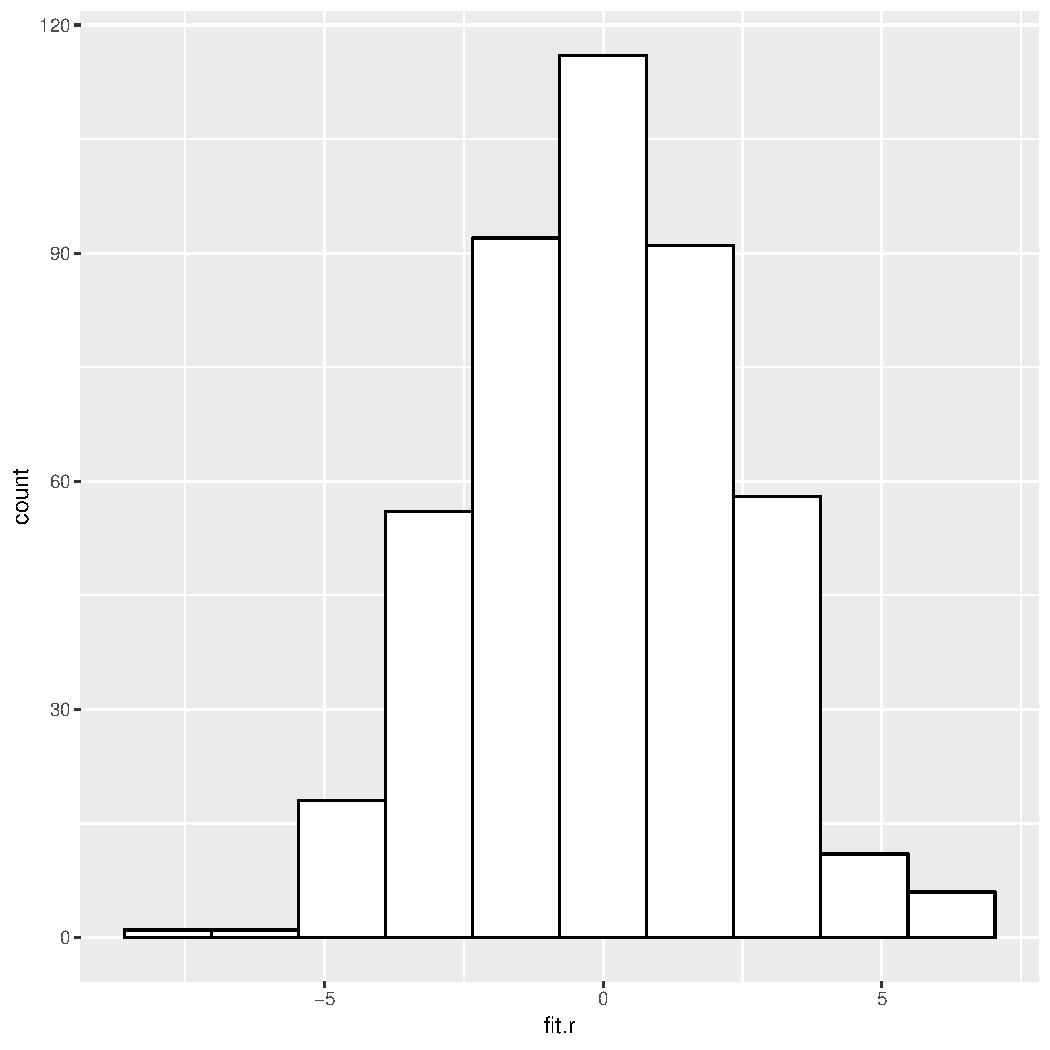
\includegraphics[width=\textwidth]{15_Diagnostics/multresidhist2.pdf} %filename
                \caption{Histogram \label{fig:multresidhist2}}
        \end{subfigure}
        \begin{subfigure}[b]{0.4\textwidth}
                \centering
                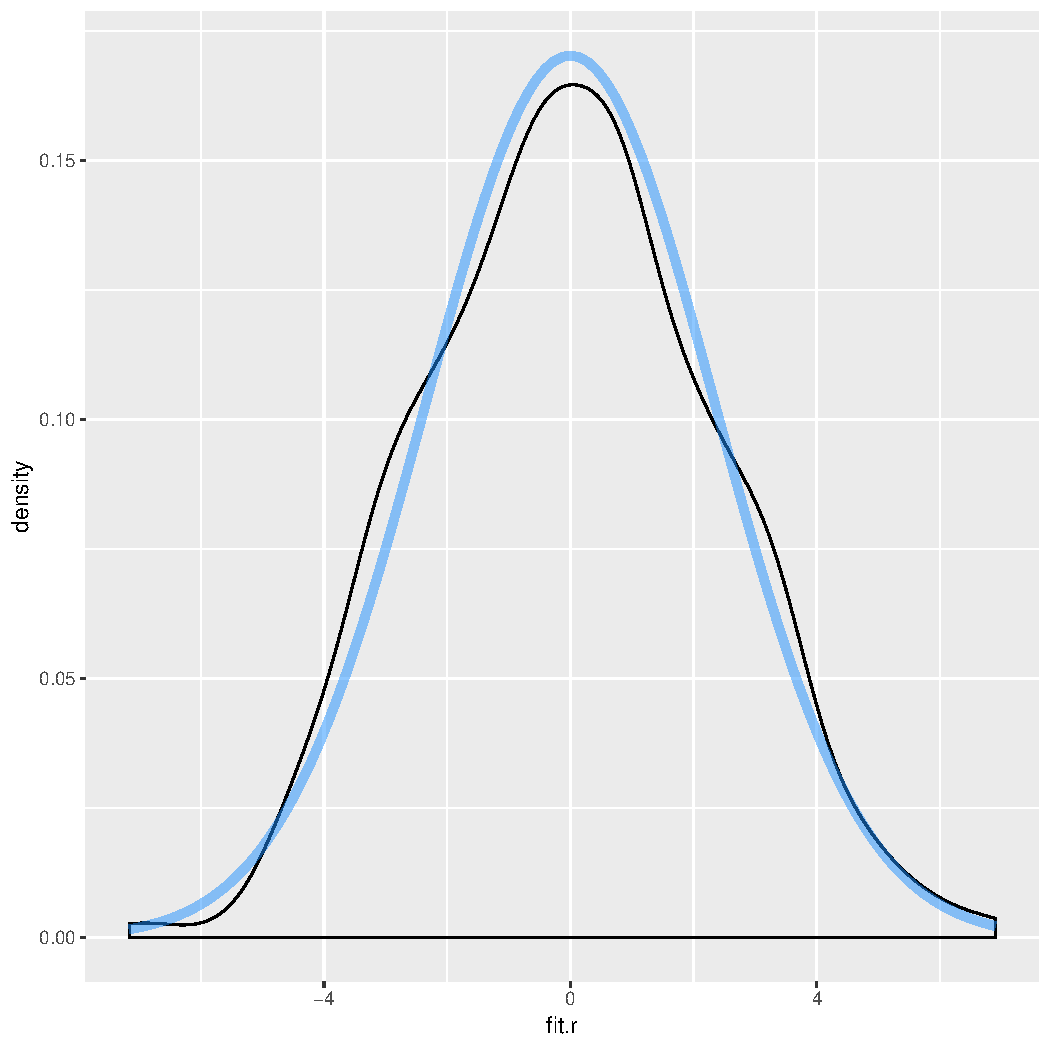
\includegraphics[width=\textwidth]{15_Diagnostics/multresidden2.pdf} %filename
                \caption{Density \label{fig:multresidden2}}
        \end{subfigure}
        \begin{subfigure}[b]{0.4\textwidth}
                \centering
                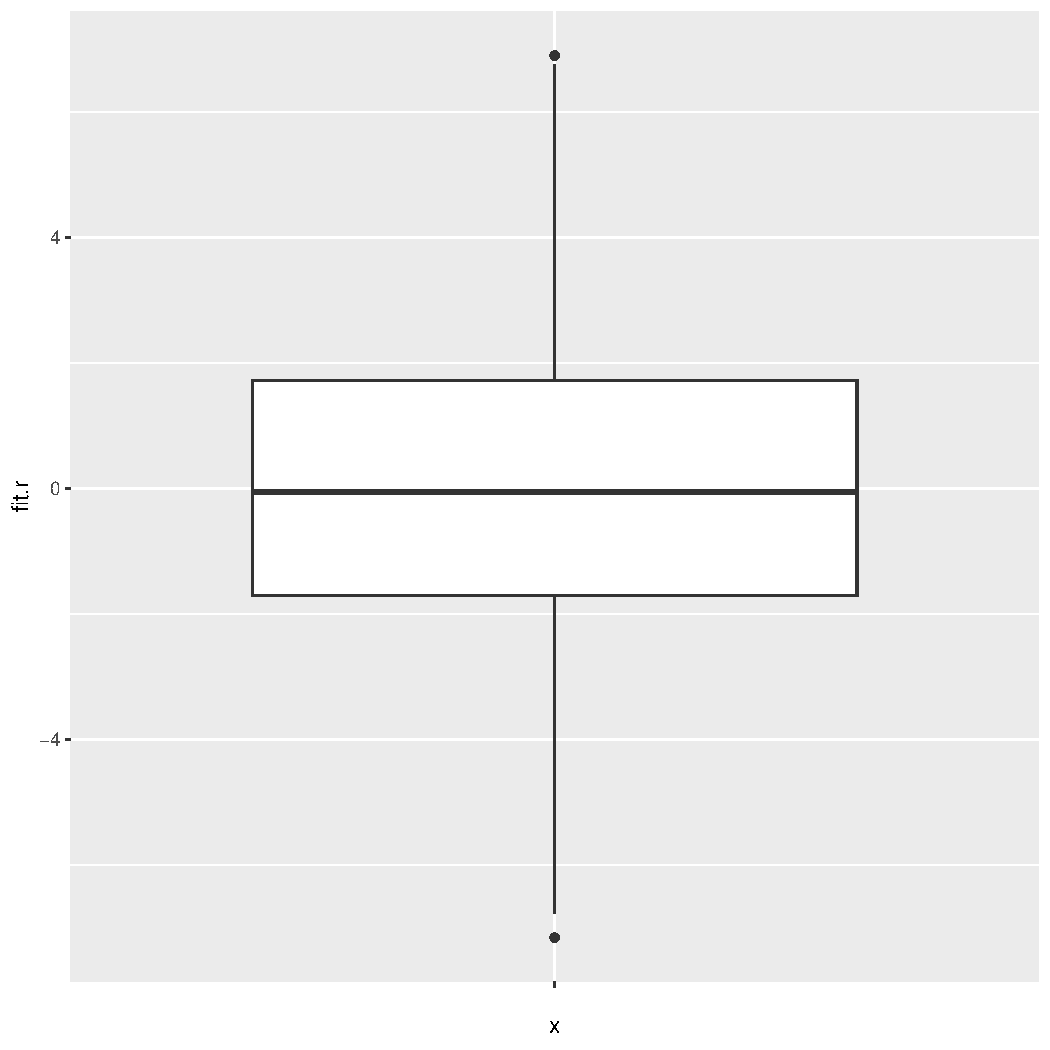
\includegraphics[width=\textwidth]{15_Diagnostics/multresidbox.pdf} %filename
                \caption{Boxplot \label{fig:multresidbox}}
        \end{subfigure}
        \begin{subfigure}[b]{0.4\textwidth}
                \centering
                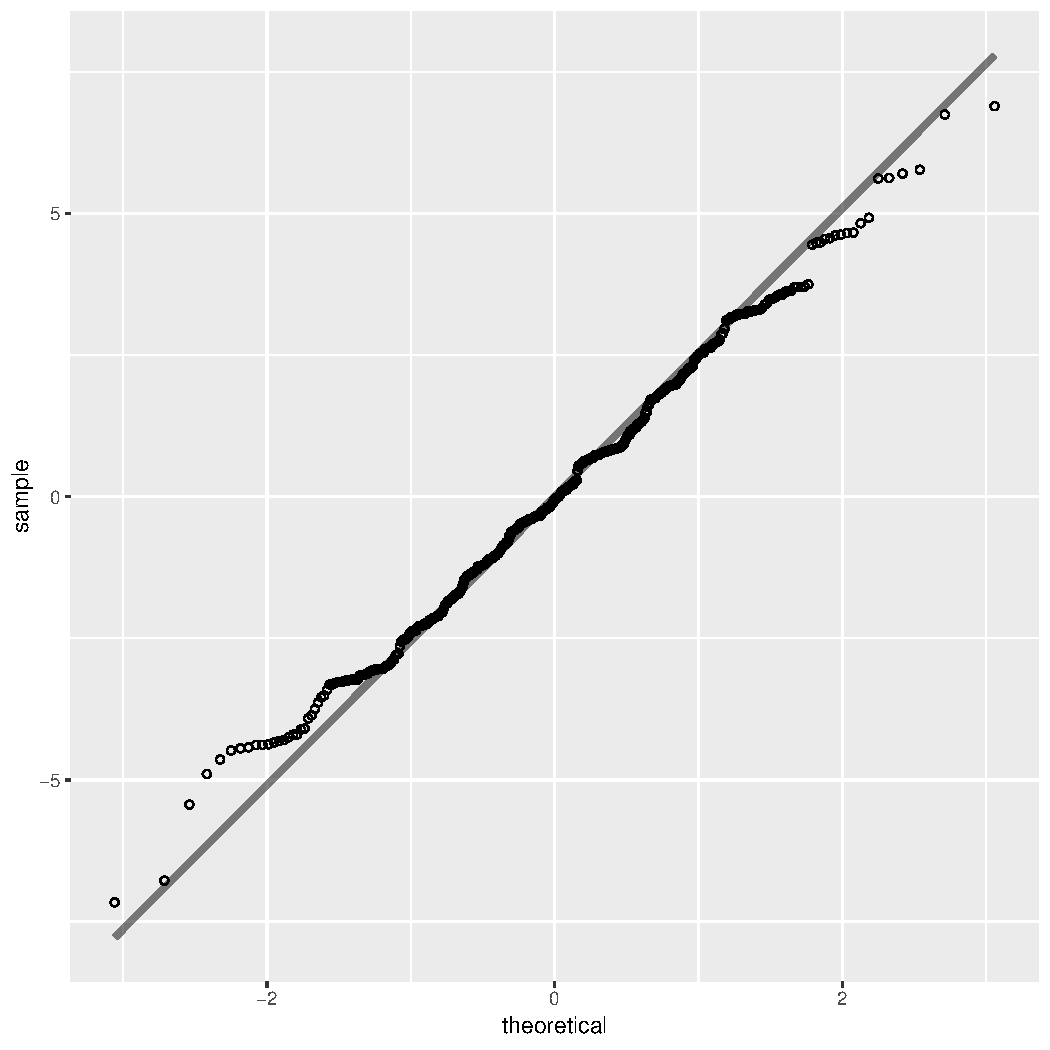
\includegraphics[width=\textwidth]{15_Diagnostics/multresidqq.pdf} %filename
                \caption{QQ Plot \label{fig:multresidqq}}
        \end{subfigure}
        \caption{Multiple Regression Residuals}
\end{figure}


It appears from the graphs, on the basis of an ``ocular test", that the residuals are potentially normally distributed.  Therefore, to perform a statistical test for non-normality, we use the Shapiro-Wilk, $W$, test statistic. $W$ is expressed as: 
\begin{equation}
  \label{eq:sw}
  W = \frac{(\sum_{i=1}^{n} a_i x_{(i)})^{2}}{\sum_{i=1}^{n} (x_i-\bar{x})^{2}}
\end{equation}
\noindent where $x_{(i)}$ are the ordered sample values and $a_i$ are constants generated from the means, variances, and covariances of the order statistics from a normal distribution. 
The Shapiro-Wilk tests the null hypothesis that the residuals are normally distributed. To perform this test in \texttt{R}, use the \texttt{shapiro.test} function.   
\begin{knitrout}
\definecolor{shadecolor}{rgb}{0.969, 0.969, 0.969}\color{fgcolor}\begin{kframe}
\begin{alltt}
\hlkwd{shapiro.test}\hlstd{(ols1}\hlopt{$}\hlstd{residuals)}
\end{alltt}
\begin{verbatim}
## 
## 	Shapiro-Wilk normality test
## 
## data:  ols1$residuals
## W = 0.99566, p-value = 0.2485
\end{verbatim}
\end{kframe}
\end{knitrout}
\noindent Since we have a relatively large $p$ value we fail to reject the null hypothesis of normally distributed errors.  Our residuals are, accoridng to our visual examination and this test, normally distributed. 

To adjust for non-normal errors we can use robust estimators, as discussed earlier with respect to heteroscedasticity. Robust estimators correct for non-normality, but produce estimated standard errors of the partial regression coefficients that tend to be larger, and hence produce less model precision. Other possible steps, where warranted, include transformation of variables that may have non-linear relationships with $Y$. Typically this involves taking log transformations of the suspect variables. 

\subsection{Outliers, Leverage, and Influence} 

Apart from the distributional behavior of residuals, it is also important to examine the residuals for ``unusual" observations. Unusual observations in the data may be cases of mis-coding (e.g., $-99$), mis-measurement, or perhaps special cases that require different kinds of treatment in the model. All of these may appear as unusual cases that are observed in your diagnostic analysis. The unusual cases that we should be most concerned about are regression outliers, that are potentially influential and that are suspect because of their differences from other cases.

Why should we worry about outliers? Recall that OLS minimizes the sum of the squared residuals for a model. Unusual cases -- which by definition will have large outliers -- have the potential to substantially influence our estimates of $B$ because their already large residuals are squared. A large outlier can thus result in OLS estimates that change the model intercept and slope.

There are several steps that can help identify outliers and their effects on your model. The first -- and most obvious -- is to examine the range of values in your $Y$ and $X$ variables. Do they fall within the appropriate ranges?

This step -- too often omitted even by experienced analysts -- can help you avoid often agonizing mis-steps that result from inclusion of miscoded data or missing values (e.g., ``-99") that need to be recoded before running your model. If you fail to identify these problems, they will show up in your residual analysis as outliers. But it is much easier to catch the problem \texttt{before} you run your model.

But sometimes we find outliers for reasons other than mis-codes, and identification requires careful examination of your residuals.  First we discuss how to find outliers -- unusual values of $Y$ -- and leverage -- unusual values of $X$ -- since they are closely related.  

\subsubsection{Outliers}

A regression outlier is an observation that has an unusual value on the dependent variable $Y$, conditioned on the values of the independent variables, $X$. Note that an outlier can have a large residual value, but not necessarily affect the estimated slope or intercept. Below we examine a few ways to identify potential outliers, and their effects on our estimated slope coefficients.   

Using the regression example, we first plot the residuals to look for any possible outliers. In this plot we are plotting the raw residuals for each of the $500$ observations. This is shown in Figure \ref{fig:siminresid}.  

% residual plot 
\begin{knitrout}
\definecolor{shadecolor}{rgb}{0.969, 0.969, 0.969}\color{fgcolor}\begin{kframe}
\begin{alltt}
\hlkwd{ggplot}\hlstd{(ds.small,} \hlkwd{aes}\hlstd{(}\hlkwd{row.names}\hlstd{(ds.small), fit.r))} \hlopt{+} \hlkwd{geom_point}\hlstd{(}\hlkwc{shape} \hlstd{=} \hlnum{1}\hlstd{)} \hlopt{+}
    \hlkwd{geom_hline}\hlstd{(}\hlkwc{yintercept} \hlstd{=} \hlnum{0}\hlstd{,} \hlkwc{color} \hlstd{=} \hlstr{"red"}\hlstd{)}
\hlkwd{dev.off}\hlstd{()}
\end{alltt}
\end{kframe}
\end{knitrout}

\begin{figure}
        \centering
       %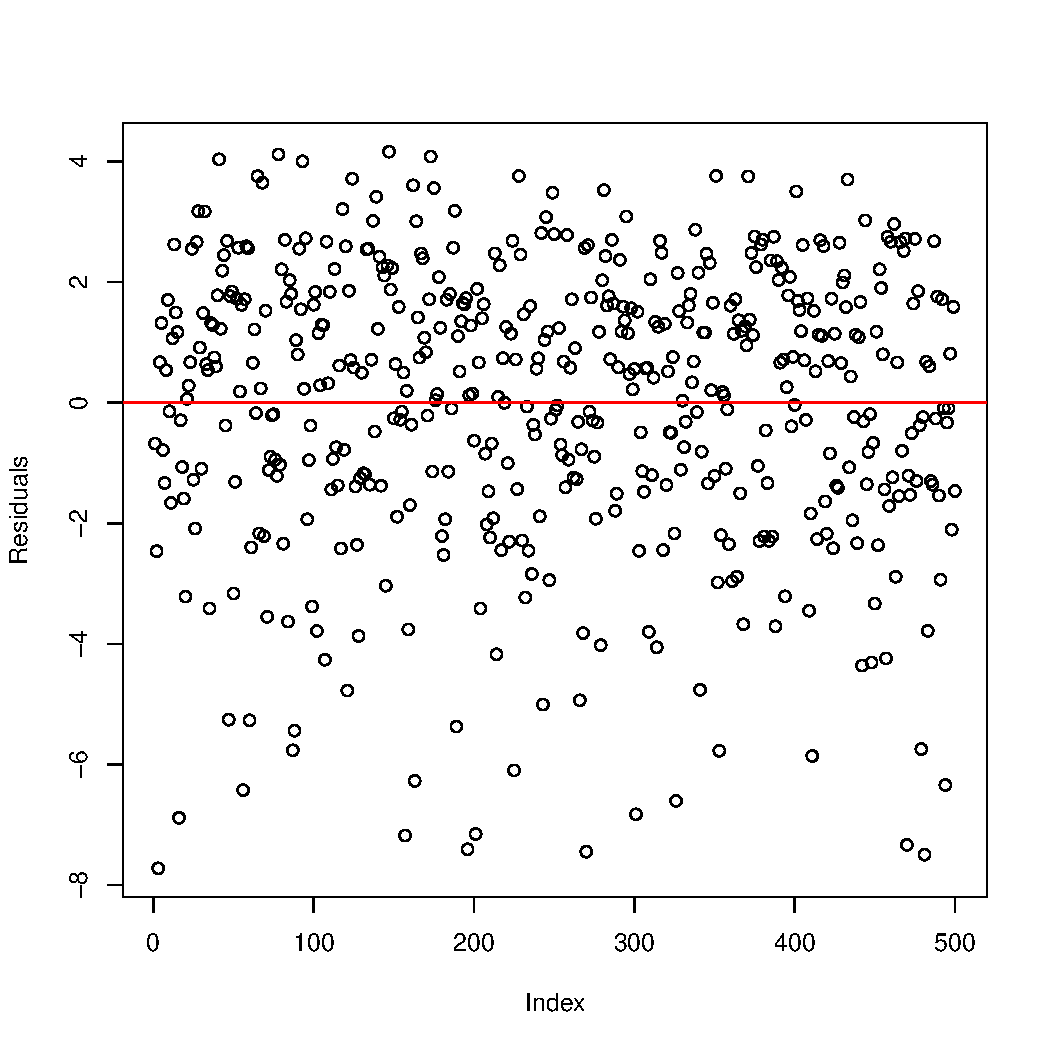
\includegraphics[width=4in]{15_Diagnostics/siminresid.pdf}%this was not dynamic
          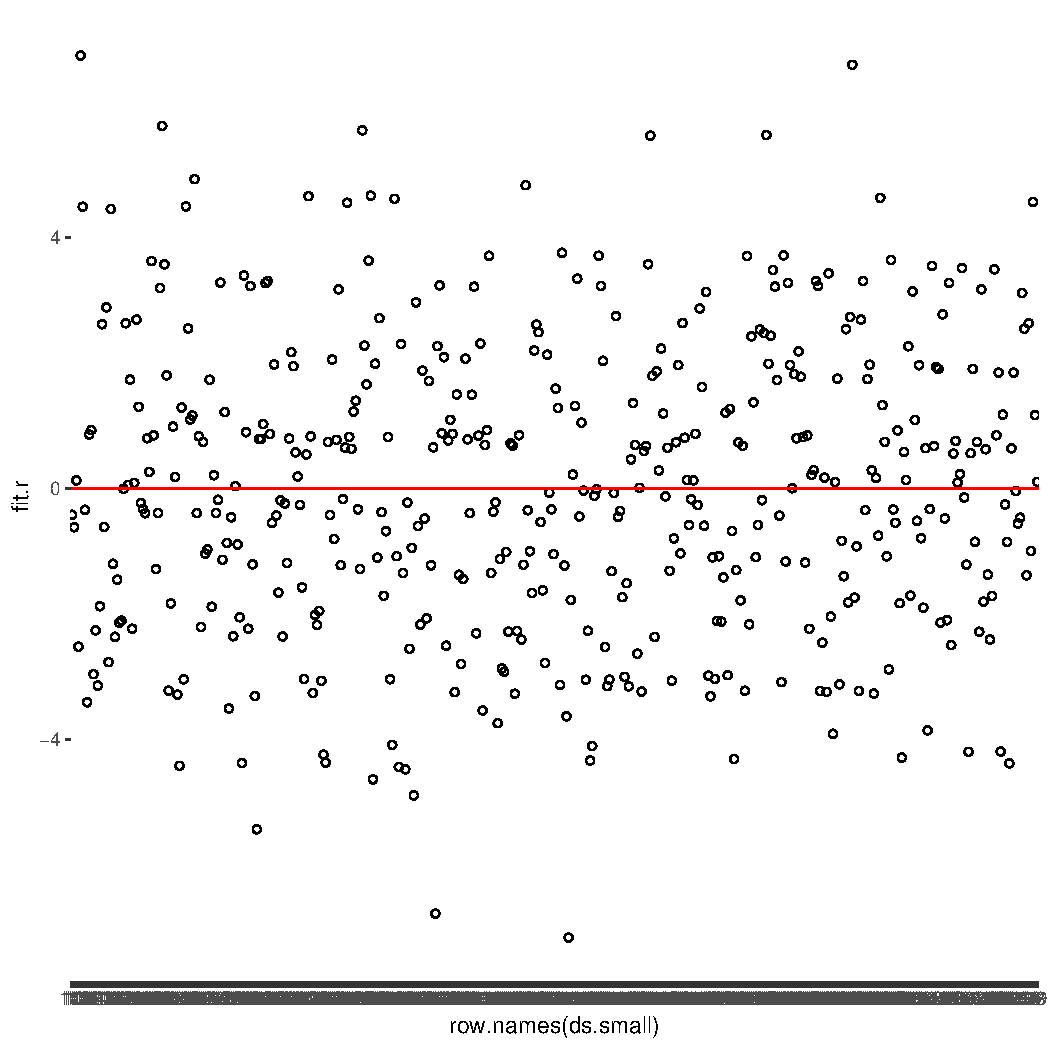
\includegraphics[width=4in]{15_Diagnostics/multinresid.pdf}%filename
        \caption{Index Plot of Residuals: Multiple Regression \label{fig:siminresid}}
\end{figure}        

%Above graphic is not generated by R chunks. -- this may be fixed

Next, we can sort the residuals and find the case with the largest absolute value and examine that case.  

% largest residuals 
\begin{knitrout}
\definecolor{shadecolor}{rgb}{0.969, 0.969, 0.969}\color{fgcolor}\begin{kframe}
\begin{alltt}
\hlcom{# Sort the residuals}
\hlstd{output.1} \hlkwb{<-} \hlkwd{sort}\hlstd{(ols1}\hlopt{$}\hlstd{residuals)}  \hlcom{# smallest first}
\hlstd{output.2} \hlkwb{<-} \hlkwd{sort}\hlstd{(ols1}\hlopt{$}\hlstd{residuals,} \hlkwc{decreasing} \hlstd{=} \hlnum{TRUE}\hlstd{)}  \hlcom{# largest first}

\hlcom{# The head function return the top results, the argument 1}
\hlcom{# returns 1 variable only}
\hlkwd{head}\hlstd{(output.1,} \hlnum{1}\hlstd{)}  \hlcom{# smallest residual absolute value}
\end{alltt}
\begin{verbatim}
##       333 
## -7.161695
\end{verbatim}
\begin{alltt}
\hlkwd{head}\hlstd{(output.2,} \hlnum{1}\hlstd{)}  \hlcom{# largest residual absolute value}
\end{alltt}
\begin{verbatim}
##      104 
## 6.898077
\end{verbatim}
\end{kframe}
\end{knitrout}

Then, we can examine the $X$ and $Y$ values of those cases on key variables. Here we examine the values across all independent variables in the model.  

\begin{knitrout}
\definecolor{shadecolor}{rgb}{0.969, 0.969, 0.969}\color{fgcolor}\begin{kframe}
\begin{alltt}
\hlstd{ds.small[}\hlkwd{c}\hlstd{(}\hlnum{298}\hlstd{,} \hlnum{94}\hlstd{),} \hlkwd{c}\hlstd{(}\hlstr{"age"}\hlstd{,} \hlstr{"education"}\hlstd{,} \hlstr{"income"}\hlstd{,} \hlstr{"ideol"}\hlstd{,}
    \hlstr{"glbcc_risk"}\hlstd{)]}  \hlcom{# [c(row numbers),c(column numbers)]}
\end{alltt}
\begin{verbatim}
##     age education income ideol glbcc_risk
## 333  69         6 100000     2          2
## 104  55         7  94000     7         10
\end{verbatim}
\end{kframe}
\end{knitrout}

By examining the case of 298, we can see that this is outlier because the observed values of $Y$ are far from what would be expected, given the values of $X$. A wealthy older liberal would most likely rate climate change as riskier than a 2. In case 94, a strong conservaitive rates climate change risk at the lowest possible value.  This observation, while not consistent with the estimated relationship between ideology and environmental concern, is certainly not implausible.  But the unusual appearance of a case with a strong conservative leaning, and high risk of cliamte change results in a large residual.

What we really want to know is: does any particular case substantially change the regression results? If a case  substantively change the results than it is said to have influence. Individual cases can be outliers, but still be influential.  Note that DFBETAS are \textbf{case statistics}, therefore a DFBETA value will be calculated for each variable for each case.   

\subsubsection{DFBETAS} 
DFBETAS measure the influence of case $i$ on the $j$ estimated coefficients. Specifically, it asks by how many standard errors does $B_j$ change when case $i$ is removed DFBETAS are expressed as:
\begin{equation}
  \label{eq:dfbeta}
  \text{DFBETAS}_{ij} = \frac{B_{j(-i)}-B_j}{SE(B_j)}
\end{equation}
Note that if DFBETAS $ > 0$, then case $i$ pulls $B_j$ \textit{up}, and  if DFBETAS $ < 0$, then case $i$ pulls $B_j$ \textit{down}.  In general, if $|\text{DFBETAS}_{ij}| > \frac{2}{\sqrt{n}}$ then these cases warrant further examination. Note that this approach gets the top 5\% of influential cases, given the sample size. For both simple (bi-variate) and  multiple regression models the DFBETA cut-offs can be calculated in \texttt{R}.  
\begin{knitrout}
\definecolor{shadecolor}{rgb}{0.969, 0.969, 0.969}\color{fgcolor}\begin{kframe}
\begin{alltt}
\hlstd{df} \hlkwb{<-} \hlnum{2}\hlopt{/}\hlkwd{sqrt}\hlstd{(}\hlnum{500}\hlstd{)}
\hlstd{df}
\end{alltt}
\begin{verbatim}
## [1] 0.08944272
\end{verbatim}
\end{kframe}
\end{knitrout}
\noindent In this case, if $|\text{DFBETAS}| > 0.0894427$ then they can be examined for  possible influence. Note, however, than in large datasets this may prove to be difficult,  so you should examine the largest DFBETAS first. In our example, we will look only at the largest 5 DFBETAS.

To calculate the DFBETAS we use the \texttt{dfbetas} function. Then we examine the DFBETA values for the first five rows of our data. 
\begin{knitrout}
\definecolor{shadecolor}{rgb}{0.969, 0.969, 0.969}\color{fgcolor}\begin{kframe}
\begin{alltt}
\hlstd{df.ols1} \hlkwb{<-} \hlkwd{dfbetas}\hlstd{(ols1)}
\hlstd{df.ols1[}\hlnum{1}\hlopt{:}\hlnum{5}\hlstd{, ]}
\end{alltt}
\begin{verbatim}
##    (Intercept)          age   education      income        ideol
## 1 -0.004396485  0.005554545  0.01043817 -0.01548697 -0.005616679
## 2  0.046302381 -0.007569305 -0.02671961 -0.01401653 -0.042323468
## 3 -0.002896270  0.018301623 -0.01946054  0.02534233 -0.023111519
## 5 -0.072106074  0.060263914  0.02966501  0.01243482  0.015464937
## 7 -0.057608817 -0.005345142 -0.04948456  0.06456577  0.134103149
\end{verbatim}
\end{kframe}
\end{knitrout}
We can then plot the DFBETAS for each of the IVs in our  regression models, and create lines for $\pm 0.089$.  Figure \ref{fig:dfbetas} shows the DFBETAS for each variable in the multiple regression model.   

\begin{knitrout}
\definecolor{shadecolor}{rgb}{0.969, 0.969, 0.969}\color{fgcolor}\begin{kframe}
\begin{alltt}
\hlkwd{melt}\hlstd{(df.ols1,} \hlkwc{varnames} \hlstd{=} \hlkwd{c}\hlstd{(}\hlstr{"index"}\hlstd{,} \hlstr{"variable"}\hlstd{))} \hlopt \hlkwd{ggplot}\hlstd{(}\hlkwd{aes}\hlstd{(index,}
    \hlstd{value))} \hlopt{+} \hlkwd{geom_point}\hlstd{()} \hlopt{+} \hlkwd{geom_hline}\hlstd{(}\hlkwc{yintercept} \hlstd{= df)} \hlopt{+} \hlkwd{geom_hline}\hlstd{(}\hlkwc{yintercept} \hlstd{=} \hlopt{-}\hlstd{df)} \hlopt{+}
    \hlkwd{facet_wrap}\hlstd{(}\hlopt{~}\hlstd{variable,} \hlkwc{scales} \hlstd{=} \hlstr{"free"}\hlstd{)}
\hlkwd{dev.off}\hlstd{()}
\end{alltt}
\end{kframe}
\end{knitrout}

\begin{figure}
        \centering
        \includegraphics[width=4in]{15_Diagnostics/dfbetas.pdf}%filename
        \caption{Index Plot of DFBETAS: Multiple  Regression \label{fig:dfbetas}}
\end{figure}        

As can be seen, several cases seem to exceed the $0.089$ cut-off. Next we find the case with the highest absolute DFBETA value, and examine the $X$ and $Y$ values for that case. 
\begin{knitrout}
\definecolor{shadecolor}{rgb}{0.969, 0.969, 0.969}\color{fgcolor}\begin{kframe}
\begin{alltt}
\hlcom{################### Return Absolute Value dfbeta}
\hlkwd{names}\hlstd{(df.ols1)} \hlkwb{<-} \hlkwd{row.names}\hlstd{(ds.small)}
\hlstd{df.ols1[}\hlkwd{abs}\hlstd{(df.ols1)} \hlopt{==} \hlkwd{max}\hlstd{(}\hlkwd{abs}\hlstd{(df.ols1))]}
\end{alltt}
\begin{verbatim}
##      <NA> 
## 0.4112137
\end{verbatim}
\begin{alltt}
\hlcom{# a observation name may not be returned - let's figure out}
\hlcom{# the observation}

\hlcom{# convert df.osl1 from matrix to dataframe}
\hlkwd{class}\hlstd{(df.ols1)}
\end{alltt}
\begin{verbatim}
## [1] "matrix"
\end{verbatim}
\begin{alltt}
\hlstd{df2.ols1} \hlkwb{<-} \hlkwd{as.data.frame}\hlstd{(df.ols1)}

\hlcom{# add an id variable}
\hlstd{df2.ols1}\hlopt{$}\hlstd{id} \hlkwb{<-} \hlnum{1}\hlopt{:}\hlnum{450}  \hlcom{#  generate a new observation number}

\hlcom{# head function returns one value, based on ,1 syntax -}
\hlcom{# head(data_set[with(data_set, order(+/-variable)), ], 1)}

\hlcom{# Ideology}
\hlkwd{head}\hlstd{(df2.ols1[}\hlkwd{with}\hlstd{(df2.ols1,} \hlkwd{order}\hlstd{(}\hlopt{-}\hlstd{ideol)), ],} \hlnum{1}\hlstd{)}  \hlcom{# order declining}
\end{alltt}
\begin{verbatim}
##      (Intercept)        age   education      income     ideol  id
## 333 -0.001083869 -0.1276632 -0.04252348 -0.07591519 0.2438799 298
\end{verbatim}
\begin{alltt}
\hlkwd{head}\hlstd{(df2.ols1[}\hlkwd{with}\hlstd{(df2.ols1,} \hlkwd{order}\hlstd{(}\hlopt{+}\hlstd{ideol)), ],} \hlnum{1}\hlstd{)}  \hlcom{# order increasing}
\end{alltt}
\begin{verbatim}
##     (Intercept)       age   education     income       ideol  id
## 148  -0.0477082 0.1279219 -0.03641922 0.04291471 -0.09833372 131
\end{verbatim}
\begin{alltt}
\hlcom{# Income}
\hlkwd{head}\hlstd{(df2.ols1[}\hlkwd{with}\hlstd{(df2.ols1,} \hlkwd{order}\hlstd{(}\hlopt{-}\hlstd{income)), ],} \hlnum{1}\hlstd{)}  \hlcom{# order declining}
\end{alltt}
\begin{verbatim}
##     (Intercept)         age    education    income       ideol  id
## 494 -0.05137992 -0.01514244 -0.009938873 0.4112137 -0.03873292 445
\end{verbatim}
\begin{alltt}
\hlkwd{head}\hlstd{(df2.ols1[}\hlkwd{with}\hlstd{(df2.ols1,} \hlkwd{order}\hlstd{(}\hlopt{+}\hlstd{income)), ],} \hlnum{1}\hlstd{)}  \hlcom{# order increasing}
\end{alltt}
\begin{verbatim}
##     (Intercept)         age  education     income      ideol  id
## 284  0.06766781 -0.06611698 0.08166577 -0.4001515 0.04501527 254
\end{verbatim}
\begin{alltt}
\hlcom{# Age}
\hlkwd{head}\hlstd{(df2.ols1[}\hlkwd{with}\hlstd{(df2.ols1,} \hlkwd{order}\hlstd{(}\hlopt{-}\hlstd{age)), ],} \hlnum{1}\hlstd{)}  \hlcom{# order declining}
\end{alltt}
\begin{verbatim}
##    (Intercept)       age  education      income     ideol id
## 87  -0.2146905 0.1786665 0.04131316 -0.01755352 0.1390403 78
\end{verbatim}
\begin{alltt}
\hlkwd{head}\hlstd{(df2.ols1[}\hlkwd{with}\hlstd{(df2.ols1,} \hlkwd{order}\hlstd{(}\hlopt{+}\hlstd{age)), ],} \hlnum{1}\hlstd{)}  \hlcom{# order increasing}
\end{alltt}
\begin{verbatim}
##     (Intercept)        age  education     income     ideol  id
## 467    0.183455 -0.2193257 -0.1906404 0.02477437 0.1832784 420
\end{verbatim}
\begin{alltt}
\hlcom{# Education - we find the amount - ID 308 for edu}
\hlkwd{head}\hlstd{(df2.ols1[}\hlkwd{with}\hlstd{(df2.ols1,} \hlkwd{order}\hlstd{(}\hlopt{-}\hlstd{education)), ],} \hlnum{1}\hlstd{)}  \hlcom{# order declining}
\end{alltt}
\begin{verbatim}
##     (Intercept)        age education      income      ideol  id
## 343  -0.1751724 0.06071469 0.1813973 -0.05557382 0.09717012 308
\end{verbatim}
\begin{alltt}
\hlkwd{head}\hlstd{(df2.ols1[}\hlkwd{with}\hlstd{(df2.ols1,} \hlkwd{order}\hlstd{(}\hlopt{+}\hlstd{education)), ],} \hlnum{1}\hlstd{)}  \hlcom{# order increasing}
\end{alltt}
\begin{verbatim}
##     (Intercept)       age  education      income        ideol id
## 105  0.05091437 0.1062966 -0.2033285 -0.02741242 -0.005880984 95
\end{verbatim}
\begin{alltt}
\hlcom{# View the output}
\hlstd{df.ols1[}\hlkwd{abs}\hlstd{(df.ols1)} \hlopt{==} \hlkwd{max}\hlstd{(}\hlkwd{abs}\hlstd{(df.ols1))]}
\end{alltt}
\begin{verbatim}
##      <NA> 
## 0.4112137
\end{verbatim}
\begin{alltt}
\hlstd{df.ols1[}\hlkwd{c}\hlstd{(}\hlnum{308}\hlstd{), ]}  \hlcom{# dfbeta number is observation 131 - education}
\end{alltt}
\begin{verbatim}
## (Intercept)         age   education      income       ideol 
## -0.17517243  0.06071469  0.18139726 -0.05557382  0.09717012
\end{verbatim}
\begin{alltt}
\hlstd{ds.small[}\hlkwd{c}\hlstd{(}\hlnum{308}\hlstd{),} \hlkwd{c}\hlstd{(}\hlstr{"age"}\hlstd{,} \hlstr{"education"}\hlstd{,} \hlstr{"income"}\hlstd{,} \hlstr{"ideol"}\hlstd{,} \hlstr{"glbcc_risk"}\hlstd{)]}
\end{alltt}
\begin{verbatim}
##     age education income ideol glbcc_risk
## 343  51         2  81000     3          4
\end{verbatim}
\end{kframe}
\end{knitrout}

Note that this ``severe outlier" is indeed an interesting case -- a 51 year old with a high school diploma, relatively high income, who is slightly liberal and perceivs low risk for climate change. But this outlier is not implausible, and therefore we can be reassured that -- even in this most extreme case -- we do not have problematic outliers.

So, having explored the residuals from our model, we found a number of outliers, some with  significant influence on our model results. In inspection of the most extreme outlier gave us no cause to worry that the observations were inappropriately distorting our model results. But what should you do if you find puzzling, implausible observations that may  influence your model?

First, as always, evaluate your theory. Is it possible that the case represented a class of observations that behave systematically differently than the other cases? This is of particular concern if you have a cluster of cases, all determined to be outliers, that have similar properties. You may need to modify your theory to account for this subgroup. One such example can be found in the study of American politics, wherein the Southern states routinely appeared to behave differently than others. Most careful efforts to model state (and individual) political behavior account for the unique aspects of southern politics, in ways ranging from the addition of dummy variables to interaction terms in regression models.

How would you determine whether the model (and theory) should be revised? Look closely at the deviant cases -- what can you learn from them? Try experiments by running the models with controls -- dummies and interaction terms. What effects do you observe? If your results suggest theoretical revisions, you will need to collect new data to test your new hypotheses. Remember: In empirical studies, you need to keep your discoveries distinct from your hypothesis tests.

As a last resort, if you have troubling outliers for which you cannot account in theory, you might decide omit those observations from your model and re-run your analyses. We do not recommend this course of action, because it can  appear to be a case of ``jiggering the data" to get the results you want. 

\subsection{Multicollinearity} 

Multicollinearity is the correlation of the IVs in the model. Note that if any $X_i$ is a linear combination of other $X$'s in the model, $B_i$ cannot be estimated. As discussed previously, the partial regression coefficient strips both the $X$'s and $Y$ of the overlapping covariation by regressing one $X$ variable on all other $X$ variables: 
\begin{align*}
  E_{X_{i}|X_{j}} &= X_i - \hat{X}_i \\
  \hat{X}_i &= A + BX_j 
\end{align*}
If an X is perfectly predicted by the other $X$'s, then:
\begin{center}
  $E_{X_{i}|X_{j}}=0$ 
  
  and 
  
  $R^2_k=1$
\end{center}
\noindent where $R^2_k$ is the $R^2$ obtained from regressing all
$X_k$ on all other $X$'s. 

We rarely find perfect multicollinearity in practice, but high multicollinearity results in loss of statistical resolution. Such as:  
\begin{itemize}
\item Large standard errors
\item Low $t$-stats, high $p$-values
  \begin{itemize}
\item This erodes the resolution of our hypothesis tests
  \end{itemize}
\item Enormous sensitivity to small changes in:
  \begin{itemize}
\item Data
\item Model specification
  \end{itemize}
  \end{itemize}

You should always check the correlations between the IVs during the model building process. This is a way to quickly identify possible multicollinearity issues.
\begin{knitrout}
\definecolor{shadecolor}{rgb}{0.969, 0.969, 0.969}\color{fgcolor}\begin{kframe}
\begin{alltt}
\hlstd{ds} \hlopt \hlkwd{select}\hlstd{(age, education, income, ideol)} \hlopt \hlkwd{na.omit}\hlstd{()} \hlopt
    \hlkwd{data.frame}\hlstd{()} \hlopt \hlkwd{cor}\hlstd{()}
\end{alltt}
\begin{verbatim}
##                   age   education      income       ideol
## age        1.00000000 -0.06370223 -0.11853753  0.08535126
## education -0.06370223  1.00000000  0.30129917 -0.13770584
## income    -0.11853753  0.30129917  1.00000000  0.04147114
## ideol      0.08535126 -0.13770584  0.04147114  1.00000000
\end{verbatim}
\end{kframe}
\end{knitrout}
\noindent There do not appear to be any variables that are so highly correlated that it would result in problems with multicolinearity. 

We will discuss two more formal ways to check for multicollinearity. First, is the  \textbf{Variance Inflation Factor} (VIF), and the second is \textbf{tolerance}. The VIF is the  degree to which the variance of other coefficients is increased due to the inclusion of the specified variable. It is expressed as: 

\begin{equation}
  \label{eq:vif}
  \text{VIF} = \frac{1}{1-R^2_k}
\end{equation}

\noindent Note that as $R^2_k$ increases the variance of $X_k$ increases. A general rule of thumb is that $\text{VIF} > 5$ is problematic. 

Another, and related, way to measure multicollinearity is tolerance. The tolerance of any $X$, $X_k$, is the proportion of its variance not shared with the other $X$'s. 
\begin{equation}
  \label{eq:tolerance}
  \text{tolerance} = 1-R^2_k 
\end{equation}

\noindent Note that this is mathematically equivalent to $\frac{1}{VIF}$. The rule of thumb for acceptable tolerance is partly a function of $n$-size:

%\begin{SingleSpace} 
 
\begin{itemize}
\item If $n < 50$, tolerance should exceed $0.7$
\item If $n < 300$, tolerance should exceed $0.5$
\item If $n < 600$, tolerance should exceed $0.3$
\item If $n < 1000$, tolerance should exceed $0.1$
\end{itemize}

%\end{SingleSpace}

%But: watch for effects on other IVs

Both VIF and tolerance can be calculated in \texttt{R}. 
\begin{knitrout}
\definecolor{shadecolor}{rgb}{0.969, 0.969, 0.969}\color{fgcolor}\begin{kframe}
\begin{alltt}
\hlkwd{library}\hlstd{(car)}
\hlkwd{vif}\hlstd{(ols1)}
\end{alltt}
\begin{verbatim}
##       age education    income     ideol 
##  1.024094  1.098383  1.101733  1.009105
\end{verbatim}
\begin{alltt}
\hlnum{1}\hlopt{/}\hlkwd{vif}\hlstd{(ols1)}
\end{alltt}
\begin{verbatim}
##       age education    income     ideol 
## 0.9764731 0.9104295 0.9076611 0.9909775
\end{verbatim}
\end{kframe}
\end{knitrout}
\noindent Note that, for our example model, we are well within acceptable limits on both VIF and tolerance. 

%% what to do 
If multicollinearity is suspected, what can you do? One option is to drop one of the highly co-linear variables. However, this may result in model mis-specification. As with other modeling considerations, you must use theory as a guide. A second option would be to add new data, thereby lessening the threat posed by multicolinearity. A third option would be to obtain data from specialized  samples that maximize independent variation in the collinear variables (e.g., elite samples may disentangle the effects of income, education, and other SES-related variables). 

Yet another strategy involves reconsidering why your data are so highly  correlated. It may be that your measures are in fact different ``indicators" of the same underlying theoretical concept. This can happen, for example, when you measure sets of attitudes that are all influenced by a more general attitude or belief system. In such a case, data scaling is a promising option. This can be accomplished by building an additive scale, or using various scaling options in $R$. Another approach would be to use techniques such as factor analysis to tease out the underlying (or ``latent") variables represented by your indicator variables. Indeed, the combination of factor analysis and regression modeling is an important and widely used approach, referred to as structural equation modeling (SEM).  But that is a topic for another book and another course.

\section{Summary}
In this chapter we have described how you can approach the diagnostic stage for OLS multiple regression analysis. We described the key threats to the necessary assumptions of OLS, and listed them and their effects in Table \ref{tab:ass}. But we also noted that diagnostics are more of an art than a simple recipe. In this business you will learn as you go, both in the analysis of a particular model (or set of models) and in the development of  your own approach and procedures. We wish you well, Grasshopper!

\part{Generalized Linear Models}





\chapter{Logit Regression} 


Logit regression is a part of a larger class of generalized linear models (GLM).   In this chapter we first briefly discuss GLMs, and then move on into a more in-depth discussion of logistic regression. Once again, the examples in this chapter use the \texttt{tbur} data set. 

\section{Generalized Linear Models} 

GLMs provide a modeling structure that can relate a linear model to response variables that do not have normal distributions. The distribution of $Y$ is assumed to belong to one of an exponential family of distributions, including the Gaussian, Binomial, and Poisson distributions.  GLMs are fit to the data by the method of maximum likelihood. 

Like OLS, GLMs contain a stochastic component and a systematic component. The systematic component is expressed as: 
\begin{equation}
  \eta = \alpha + \beta_1 X_{i1} + \beta_2 X_{i2} + \ldots + \beta_k X_{ik}
\end{equation}
However, GLMs also contain a ``link function" that relates the response variable, $Y_i$, to the systematic linear component, $\eta$.  Table 16.1 shows the major exponential “families” of GLM models, and indicates the kinds of link functions involved in each.  Note that OLS models would fall within the Gaussian family.  In the next section we focus on the binomial family, and on logit estimation in particular.

\begin{figure}
        \centering
        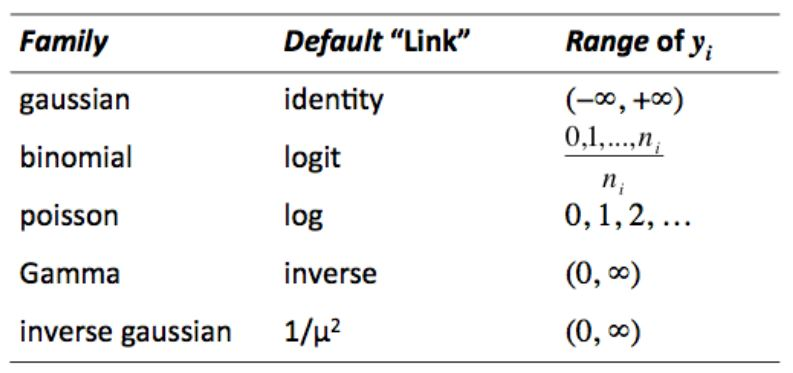
\includegraphics[width=4in]{16_Logit/families.jpg}%filename
        \caption{Exponential ``families" of GLM Models}
\end{figure} 
 

\section{Logit Estimation} 

Logit is used when predicting limited dependent variables,
specifically those in which $Y$ is represented by $0$’s and $1$’s.
By virtue of the binary dependent variable, these models do not meet the
key assumptions of OLS. Logit uses maximum likelihood estimation (MLE),
which is a counterpart to minimizing least squares. 
MLE identifies the probability of obtaining the sample as a function
of the model parameters (i.e., the $X$’s). It answers the question, 
what are the values for $B$’s that make the sample most likely? In
other words, the likelihood 
function expresses the probability of obtaining the observed data as a
function of the model parameters. Estimates of $A$ and $B$ are based
on maximizing a likelihood function of the observed $Y$ values.  
In logit estimation we seek $P(Y=1)$, the probability that $Y=1$. The
odds that $Y=1$ is expressed as:

\begin{equation*}
  O(Y=1)=\frac{P(Y=1)}{1-P(Y=1)}
\end{equation*}

\noindent Logits, $L$, are the natural logarithm of the odds: 

\begin{align*}
  L &= log_e O \\
  &=log_e \frac{P}{1-P}
\end{align*}

\noindent They can range from $-\infty$, when $P=0$, to $\infty$, when
$P=1$. $L$ is the estimated systematic linear component: 

\begin{equation*}
  L = A+B_1 X_{i1}+\ldots+B_k X_{ik}
\end{equation*}

\noindent By reversing the logit we can obtain the predicted
probability that $Y=1$ for each of the $i$ observations. 

\begin{equation}
  \label{eq:predprob}
  P_{i} = \frac{1}{1-e^{-L_{i}}}
\end{equation}

\noindent where $e=2.71828 \ldots$, the base number of natural
logarithms. Note that $L$ is a linear function, but $P$ is a non-linear
$S$-shaped function as shown in Figure \ref{fig:logex}. Also note,
that Equation 16.2 is the link function that relates the
linear component to the non-linear response variable.  
%  removed this and did a hard code; could not figure out the problem.
%  \ref{eq:predprob}

\begin{figure}
        \centering
        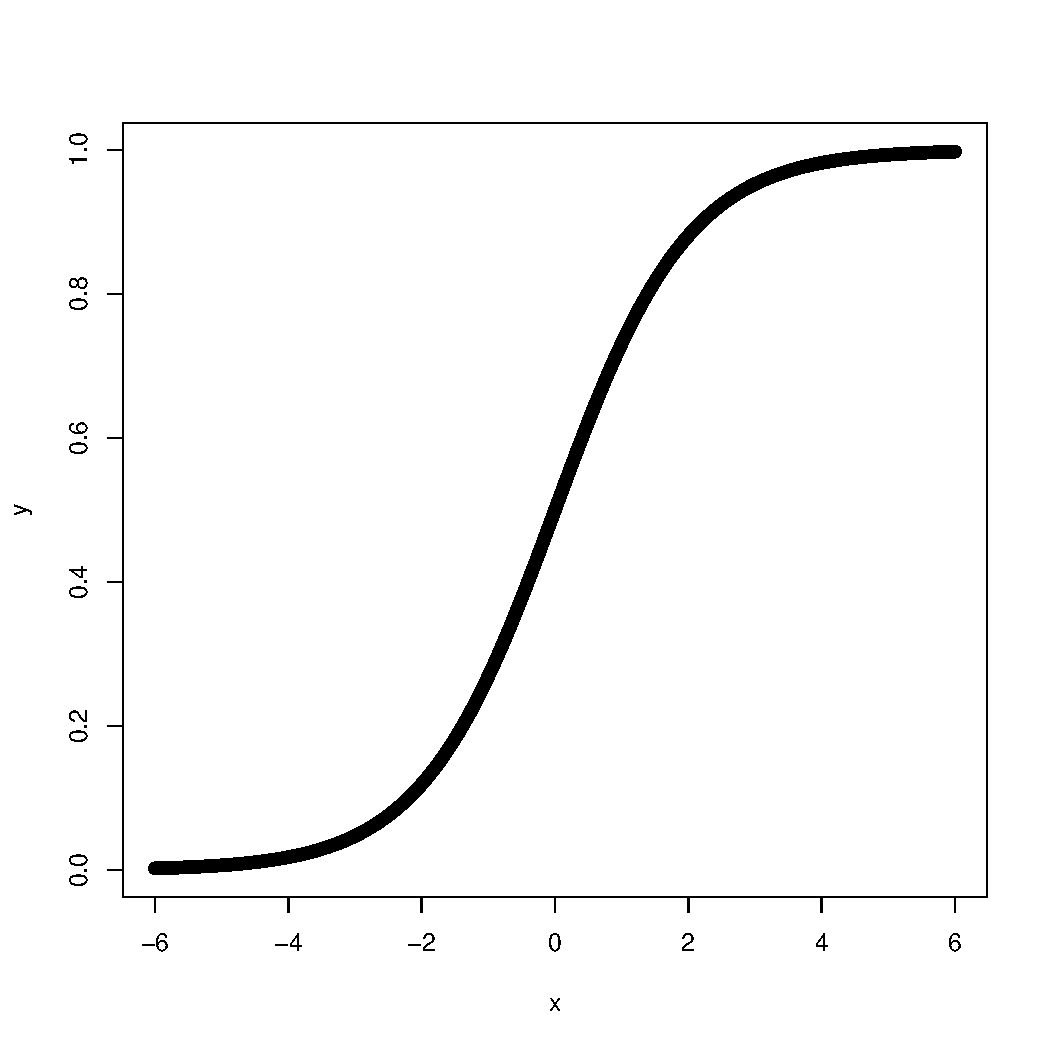
\includegraphics[width=4in]{16_Logit/logex.pdf}%filename
        \caption{Predicted Probability as a Logit Function of $X$ \label{fig:logex}}
\end{figure}   

In more formal terms, each observation, $i$,  contributes to the likelihood function by $P_i$ if $Y_i=1$, and by $1-P_i$ if $Y_i=0$. This is defined as: 
\begin{equation*}
  P^{Y_{i}}_i(1-P_i)^{1-Y_i}
\end{equation*}
\noindent The likelihood function is the product (multiplication) of all these individual contributions:
\begin{equation*}
  \ell = \prod P^{Y_{i}}_i(1-P_i)^{1-Y_i}
\end{equation*}
\noindent The likelihood function is the largest for the model that best predicts $Y=1$ or $Y=0$, therefore when the predicted value of $Y$ is correct and close to $1$ or $0$, the likelihood function is maximized. 

To estimate the model parameters, we seek to maximize the log of the likelihood function. We use the log because it converts the multiplication into addition, and is therefore easier to calculate. The log likelihood is:
\begin{equation*}
  \text{log}_e \ell = \sum^{n}_{i=1}[Y_i \text{log}_e P_i+(1-Y_i)\text{log}_e(1-P_i)]
\end{equation*}

The solution involves taking the first derivative of the log likelihood with respect to each of the $B$’s, setting them to zero, and solving the simultaneous equation.  The solution of the equation isn't linear, so it can't be solved directly.  Instead, it's solved through a sequential estimation process that looks for successively better ``fits'' of the model. 

For the most part, the key assumptions required for logit models are analogous to those required for OLS. The key differences are that (a) we do not assume a linear relationship between the $X$s and $Y$, and (b) we do not assume normally distributed, homoscedastistic residuals. The key assumptions that are retained are shown below.

\begin{grbox}
\greybox{\textbf{Logit Assumptions and Qualifiers}   
\begin{itemize}
\item The model is correctly specified
\begin{itemize}
\item True conditional probabilities are logistic function of the $X$’s
\item No important $X$’s omitted; no extraneous $X$’s included
\item No significant measurement error
\end{itemize}  
\item The cases are independent
\item No $X$ is a linear function of other $X$’s
\begin{itemize}
\item Increased multicollinearity leads to greater imprecision
\end{itemize}
\item Influential cases can bias estimates
\item Sample size: $n-k-1$ should exceed $100$ 
  \begin{itemize}
\item Independent covariation between the $X$s and $Y$ is critical
  \end{itemize}
  \end{itemize}}
\end{grbox}

 
The following example uses demographic information to predict beliefs about anthropogenic climate change. 



\begin{knitrout}
\definecolor{shadecolor}{rgb}{0.969, 0.969, 0.969}\color{fgcolor}\begin{kframe}
\begin{alltt}
\hlstd{logit1} \hlkwb{<-} \hlkwd{glm}\hlstd{(glbcc} \hlopt{~} \hlstd{age} \hlopt{+} \hlstd{gender} \hlopt{+} \hlstd{education} \hlopt{+} \hlstd{income,} \hlkwc{data} \hlstd{= ds.temp,}
    \hlkwc{family} \hlstd{=} \hlkwd{binomial}\hlstd{())}
\hlkwd{summary}\hlstd{(logit1)}
\end{alltt}
\begin{verbatim}
## 
## Call:
## glm(formula = glbcc ~ age + gender + education + income, family = binomial(), 
##     data = ds.temp)
## 
## Deviance Residuals: 
##    Min      1Q  Median      3Q     Max  
## -1.707  -1.250   0.880   1.053   1.578  
## 
## Coefficients:
##                  Estimate    Std. Error z value       Pr(>|z|)    
## (Intercept)  0.4431552007  0.2344093710   1.891       0.058689 .  
## age         -0.0107882966  0.0031157929  -3.462       0.000535 ***
## gender      -0.3131329979  0.0880376089  -3.557       0.000375 ***
## education    0.1580178789  0.0251302944   6.288 0.000000000322 ***
## income      -0.0000023799  0.0000008013  -2.970       0.002977 ** 
## ---
## Signif. codes:  0 '***' 0.001 '**' 0.01 '*' 0.05 '.' 0.1 ' ' 1
## 
## (Dispersion parameter for binomial family taken to be 1)
## 
##     Null deviance: 3114.5  on 2281  degrees of freedom
## Residual deviance: 3047.4  on 2277  degrees of freedom
## AIC: 3057.4
## 
## Number of Fisher Scoring iterations: 4
\end{verbatim}
\end{kframe}
\end{knitrout}
\noindent As we can see age and gender are both negative and statistically significant predictors of climate change opinion. Below we discuss logit hypothesis tests, goodness of fit, and how to interpret the logit coefficients.  

\subsection{Logit Hypothesis Tests} 

In some ways, hypothesis testing with logit is quite similar to that using OLS. The same use of  $p$-values is employed, however they differ in
how they are derived. The logit analysis makes use of the Wald $z$-statistic, which is similar to the $t$-stat in OLS. The Wald $z$ score compares the estimated coefficient to the asymptotic standard error, (aka the normal distribution). The $p$-value is derived from the asymptotic standard-normal distribution. Each estimated coefficient has a Wald $z$-score and a $p$-value that shows the probability that the null hypothesis is correct, given the data. 
\begin{equation}
  \label{eq:wald}
  z = \frac{B_j}{SE(B_j)} 
\end{equation}
 
\subsection{Goodness of Fit} 

Given that logit regression is estimated using MLE, the goodness-of-fit statistics differ from those of OLS. Here we examine three
measures of fit: log-likelihood, the pseudo $R^2$, and the Akaike information criteria (AIC). 

\subsubsection{Log-Likelihood}
To test for the overall null hypothesis that all $B$’s are equal to zero, similar to an overall $F$-test in OLS, we can compare the log-likelihood of the demographic model with 4 IVs to the initial ``null model" which includes only the intercept term. In general, a smaller log-likelihood indicates a better fit. Using the deviance statistic $G^2$ (aka the likelihood-ratio test statistic), we can determine whether the difference
is statistically significant. $G^2$ is expressed as: 

 \begin{equation}
   \label{eq:G}
   G^2 = 2(\text{log}_e L_1 - \text{log}_e L_0)
\end{equation}

\noindent where $L_1$ is the demographic model and $L_0$ is the null model. The $G^2$ test statistic takes the difference between the log likelihoods of the two models and compares that to a $\chi^2$ distribution with $q$ degrees of freedom, where $q$ is the difference in the number of IVs. We can calculate this in \texttt{R}.  First, we run a null model predicting belief that greenhouse gases are causing the climate to change, using only
the intercept:

\begin{knitrout}
\definecolor{shadecolor}{rgb}{0.969, 0.969, 0.969}\color{fgcolor}\begin{kframe}
\begin{alltt}
\hlstd{logit0} \hlkwb{<-} \hlkwd{glm}\hlstd{(glbcc} \hlopt{~} \hlnum{1}\hlstd{,} \hlkwc{data} \hlstd{= ds.temp)}
\hlkwd{summary}\hlstd{(logit0)}
\end{alltt}
\begin{verbatim}
## 
## Call:
## glm(formula = glbcc ~ 1, data = ds.temp)
## 
## Deviance Residuals: 
##     Min       1Q   Median       3Q      Max  
## -0.5732  -0.5732   0.4268   0.4268   0.4268  
## 
## Coefficients:
##             Estimate Std. Error t value            Pr(>|t|)    
## (Intercept)  0.57318    0.01036   55.35 <0.0000000000000002 ***
## ---
## Signif. codes:  0 '***' 0.001 '**' 0.01 '*' 0.05 '.' 0.1 ' ' 1
## 
## (Dispersion parameter for gaussian family taken to be 0.2447517)
## 
##     Null deviance: 558.28  on 2281  degrees of freedom
## Residual deviance: 558.28  on 2281  degrees of freedom
## AIC: 3267.1
## 
## Number of Fisher Scoring iterations: 2
\end{verbatim}
\end{kframe}
\end{knitrout}

We then calculate the log likelihood for the null model, 
\begin{equation}\text{log}_e L_0\end{equation}

\begin{knitrout}
\definecolor{shadecolor}{rgb}{0.969, 0.969, 0.969}\color{fgcolor}\begin{kframe}
\begin{alltt}
\hlkwd{logLik}\hlstd{(logit0)}
\end{alltt}
\begin{verbatim}
## 'log Lik.' -1631.548 (df=2)
\end{verbatim}
\end{kframe}
\end{knitrout}

Next, we calculate the log likelihood for the demographic model, 

\begin{equation}\text{log}_e L_0\end{equation}

Recall that we generated this model (dubbed ``logit1") earlier:

\begin{knitrout}
\definecolor{shadecolor}{rgb}{0.969, 0.969, 0.969}\color{fgcolor}\begin{kframe}
\begin{alltt}
\hlkwd{logLik}\hlstd{(logit1)}
\end{alltt}
\begin{verbatim}
## 'log Lik.' -1523.724 (df=5)
\end{verbatim}
\end{kframe}
\end{knitrout}

Finally, we calculate the  $G$ statistic and perform the chi-square test for statistical significance:

\begin{knitrout}
\definecolor{shadecolor}{rgb}{0.969, 0.969, 0.969}\color{fgcolor}\begin{kframe}
\begin{alltt}
\hlstd{G} \hlkwb{<-} \hlnum{2} \hlopt{*} \hlstd{(}\hlopt{-}\hlnum{1523} \hlopt{-} \hlstd{(}\hlopt{-}\hlnum{1631}\hlstd{))}
\hlstd{G}
\end{alltt}
\begin{verbatim}
## [1] 216
\end{verbatim}
\begin{alltt}
\hlkwd{pchisq}\hlstd{(G,} \hlkwc{df} \hlstd{=} \hlnum{3}\hlstd{,} \hlkwc{lower.tail} \hlstd{=} \hlnum{FALSE}\hlstd{)}
\end{alltt}
\begin{verbatim}
## [1] 0.0000000000000000000000000000000000000000000001470144
\end{verbatim}
\end{kframe}
\end{knitrout}

\noindent We can see by the very low p-value that the demographic model offers a significant improvement in fit. 

The same approach can be used to compare nested models, similar to nested $F$-tests in OLS. For example, we can include ideology in the model and use the \texttt{anova} function to see if the ideology variable improves model fit. Note that we specify the $\chi^2$ test. 
\begin{knitrout}
\definecolor{shadecolor}{rgb}{0.969, 0.969, 0.969}\color{fgcolor}\begin{kframe}
\begin{alltt}
\hlstd{logit2} \hlkwb{<-} \hlkwd{glm}\hlstd{(glbcc} \hlopt{~} \hlstd{age} \hlopt{+} \hlstd{gender} \hlopt{+} \hlstd{education} \hlopt{+} \hlstd{income} \hlopt{+} \hlstd{ideol,}
    \hlkwc{family} \hlstd{=} \hlkwd{binomial}\hlstd{(),} \hlkwc{data} \hlstd{= ds.temp)}
\hlkwd{summary}\hlstd{(logit2)}
\end{alltt}
\begin{verbatim}
## 
## Call:
## glm(formula = glbcc ~ age + gender + education + income + ideol, 
##     family = binomial(), data = ds.temp)
## 
## Deviance Residuals: 
##     Min       1Q   Median       3Q      Max  
## -2.6661  -0.8939   0.3427   0.8324   2.0212  
## 
## Coefficients:
##                  Estimate    Std. Error z value             Pr(>|z|)    
## (Intercept)  4.0545788430  0.3210639034  12.629 < 0.0000000000000002 ***
## age         -0.0042866683  0.0036304540  -1.181             0.237701    
## gender      -0.2044012213  0.1022959122  -1.998             0.045702 *  
## education    0.1009422741  0.0293429371   3.440             0.000582 ***
## income      -0.0000010425  0.0000008939  -1.166             0.243485    
## ideol       -0.7900118618  0.0376321895 -20.993 < 0.0000000000000002 ***
## ---
## Signif. codes:  0 '***' 0.001 '**' 0.01 '*' 0.05 '.' 0.1 ' ' 1
## 
## (Dispersion parameter for binomial family taken to be 1)
## 
##     Null deviance: 3114.5  on 2281  degrees of freedom
## Residual deviance: 2404.0  on 2276  degrees of freedom
## AIC: 2416
## 
## Number of Fisher Scoring iterations: 4
\end{verbatim}
\begin{alltt}
\hlkwd{anova}\hlstd{(logit1, logit2,} \hlkwc{test} \hlstd{=} \hlstr{"Chisq"}\hlstd{)}
\end{alltt}
\begin{verbatim}
## Analysis of Deviance Table
## 
## Model 1: glbcc ~ age + gender + education + income
## Model 2: glbcc ~ age + gender + education + income + ideol
##   Resid. Df Resid. Dev Df Deviance              Pr(>Chi)    
## 1      2277     3047.4                                      
## 2      2276     2404.0  1   643.45 < 0.00000000000000022 ***
## ---
## Signif. codes:  0 '***' 0.001 '**' 0.01 '*' 0.05 '.' 0.1 ' ' 1
\end{verbatim}
\end{kframe}
\end{knitrout}
\noindent As we can see, adding ideology significantly improves the model. 

\subsubsection{Pseudo $R^2$}

A measure that is equivalent to the $R^2$ in OLS does not exist for logit. Remember that explaining variance in $Y$ is not the goal of MLE. However, a ``pseudo'' $R^2$ measure exists that compares the residual deviance of the null model with that of the  full model. Like the $R^2$ measure, pseudo $R^2$ ranges from $0$ to $1$ with values closer to $1$ indicating improved model fit. 

Deviance is analogous to the residual sum of squares for a linear model. It is expressed as:

\begin{equation}
  \label{eq:dev}
  \text{deviance} = -2(\text{log}_e L)
\end{equation}

\noindent It is simply the log-likelihood of the model multiplied by a $-2$. The pseudo $R^2$ is $1$ minus the ratio of the deviance of the full model $L_1$ to the deviance of the null model $L_0$:

\begin{equation}
  \label{eq:psR2}
  \text{pseudo} R^2 = 1-\frac{-2(\text{log}_e L_1)}{-2(\text{log}_e L_0)} 
\end{equation}
\noindent This can be calculated in \texttt{R} using the full
model with ideology. 
\begin{knitrout}
\definecolor{shadecolor}{rgb}{0.969, 0.969, 0.969}\color{fgcolor}\begin{kframe}
\begin{alltt}
\hlstd{pseudoR2} \hlkwb{<-} \hlnum{1} \hlopt{-} \hlstd{(logit2}\hlopt{$}\hlstd{deviance}\hlopt{/}\hlstd{logit2}\hlopt{$}\hlstd{null.deviance)}
\hlstd{pseudoR2}
\end{alltt}
\begin{verbatim}
## [1] 0.2281165
\end{verbatim}
\end{kframe}
\end{knitrout}
\noindent The pseudo $R^2$ of the model is 0.2281165. Note that the 0.2281165 is only an approximation of explained variance, and should be used in combination with other measures of fit such as AIC.

\subsubsection{Akaike Information Criteria}
Another way to examine goodness-of-fit is the Akaike information criteria (AIC). Like the adjusted $R^2$ for OLS, the AIC takes into account the parsimony of the model by penalizing for the number of parameters. But AIC is useful only in a comparative manner -- either with the null model or an alternative model. It does not purport to describe the percent of variance in $Y$ accounted for, as does the pseudo $R^2$.

AIC is defined as -2 times the residual deviance of the model plus two times the number of parameters; $k$ IVs plus the intercept:

\begin{equation}
  \label{eq:aic}
  \text{AIC} = -2(\text{log}_e L) + 2(k+1) 
\end{equation}

\noindent Note that smaller values are indicative of a better fit. The AIC is most useful when comparing the fit of alternative (not necessarily nested) models. In $R$, AIC is given as part of the \texttt{summary} output for a \texttt{glm} object, but we can also calculate it and verify. 

\begin{knitrout}
\definecolor{shadecolor}{rgb}{0.969, 0.969, 0.969}\color{fgcolor}\begin{kframe}
\begin{alltt}
\hlstd{aic.logit2} \hlkwb{<-} \hlstd{logit2}\hlopt{$}\hlstd{deviance} \hlopt{+} \hlnum{2} \hlopt{*} \hlnum{6}
\hlstd{aic.logit2}
\end{alltt}
\begin{verbatim}
## [1] 2416.002
\end{verbatim}
\begin{alltt}
\hlstd{logit2}\hlopt{$}\hlstd{aic}
\end{alltt}
\begin{verbatim}
## [1] 2416.002
\end{verbatim}
\end{kframe}
\end{knitrout}

\subsection{Interpreting Logits} 

The logits, $L$, are logged odds, and therefore the coefficients that are produced must be interpreted as logged odds. This means that for each unit change in ideology the predicted logged odds of believing climate change has an anthropogenic cause decrease by -0.7900119. This interpretation, through mathematically straightforward, is not terribly informative. Below we discuss two ways to make the interpretation of logit analysis more intuitive.   

\subsubsection{Calculate Odds}
 
Logits can be used to directly calculate odds by taking the antilog of any of the coefficients: 
\begin{equation*}
  \textit{anti}\text{log} = e^B 
\end{equation*}
\noindent For example, the following retuns odds for all the IVs.
\begin{knitrout}
\definecolor{shadecolor}{rgb}{0.969, 0.969, 0.969}\color{fgcolor}\begin{kframe}
\begin{alltt}
\hlstd{logit2} \hlopt \hlkwd{coef}\hlstd{()} \hlopt \hlkwd{exp}\hlstd{()}
\end{alltt}
\begin{verbatim}
## (Intercept)         age      gender   education      income       ideol 
##  57.6608736   0.9957225   0.8151353   1.1062128   0.9999990   0.4538394
\end{verbatim}
\end{kframe}
\end{knitrout}
\noindent Therefore, for each 1-unit increase in the ideology scale (i.e., becoming more conservative) the odds of believing that climate change is human caused decrease by 0.4538394. 

\subsubsection{Predicted Probabilities}

The most straightforward way to interpret logits is to Equation \ref{eq:predprob}. To calculate the effect of a particular independent variable, $X_i$, on the probability of $Y = 1$, set all $X_j$'s at their means, then calculate:

\begin{equation*}
\label{eq:predprob}
  \hat{P} = \frac{1}{1+e^{-\hat{L}}}
\end{equation*}

\noindent We can then evaluate the change in predicted probabilities that $Y$=1 across the range of values in $X_i$.

This procedure can be demonstrated in a two steps. First, create a data frame holding all the variables except ideology at their mean. Second, use the \texttt{augment} function to calculate the predicted probabilities for each level of ideology. Indicate \texttt{type.predict = "response"}. 

\begin{knitrout}
\definecolor{shadecolor}{rgb}{0.969, 0.969, 0.969}\color{fgcolor}\begin{kframe}
\begin{alltt}
\hlstd{log.data} \hlkwb{<-} \hlkwd{data.frame}\hlstd{(}\hlkwc{age} \hlstd{=} \hlkwd{mean}\hlstd{(ds.temp}\hlopt{$}\hlstd{age),} \hlkwc{gender} \hlstd{=} \hlkwd{mean}\hlstd{(ds.temp}\hlopt{$}\hlstd{gender),}
    \hlkwc{education} \hlstd{=} \hlkwd{mean}\hlstd{(ds.temp}\hlopt{$}\hlstd{education),} \hlkwc{income} \hlstd{=} \hlkwd{mean}\hlstd{(ds.temp}\hlopt{$}\hlstd{income),}
    \hlkwc{ideol} \hlstd{=} \hlnum{1}\hlopt{:}\hlnum{7}\hlstd{)}
\hlstd{log.data} \hlkwb{<-} \hlstd{logit2} \hlopt \hlkwd{augment}\hlstd{(}\hlkwc{newdata} \hlstd{= log.data,} \hlkwc{type.predict} \hlstd{=} \hlstr{"response"}\hlstd{)}
\hlstd{log.data}
\end{alltt}
\begin{verbatim}
## # A tibble: 7 x 7
##     age gender education income ideol .fitted .se.fit
## * <dbl>  <dbl>     <dbl>  <dbl> <int>   <dbl>   <dbl>
## 1  60.1  0.412      5.09 70627.     1   0.967 0.00523
## 2  60.1  0.412      5.09 70627.     2   0.929 0.00833
## 3  60.1  0.412      5.09 70627.     3   0.856 0.0115 
## 4  60.1  0.412      5.09 70627.     4   0.730 0.0127 
## 5  60.1  0.412      5.09 70627.     5   0.551 0.0124 
## 6  60.1  0.412      5.09 70627.     6   0.357 0.0139 
## 7  60.1  0.412      5.09 70627.     7   0.202 0.0141
\end{verbatim}
\end{kframe}
\end{knitrout}

The output shows, for each case, the ideology measure for the respondent followed by the estimated probability ($p$) that the individual believes man-made greenhouse gasses are causing climate change.  We can also graph the results, with $95\%$ confidence intervals. This is shown in Figure \ref{fig:logitplot}.

\begin{knitrout}
\definecolor{shadecolor}{rgb}{0.969, 0.969, 0.969}\color{fgcolor}\begin{kframe}
\begin{alltt}
\hlstd{log.df} \hlkwb{<-} \hlstd{log.data} \hlopt \hlkwd{mutate}\hlstd{(}\hlkwc{upper} \hlstd{= .fitted} \hlopt{+} \hlnum{1.96} \hlopt{*} \hlstd{.se.fit,}
    \hlkwc{lower} \hlstd{= .fitted} \hlopt{-} \hlnum{1.96} \hlopt{*} \hlstd{.se.fit)}

\hlkwd{ggplot}\hlstd{(log.df,} \hlkwd{aes}\hlstd{(ideol, .fitted))} \hlopt{+} \hlkwd{geom_point}\hlstd{()} \hlopt{+} \hlkwd{geom_errorbar}\hlstd{(}\hlkwd{aes}\hlstd{(}\hlkwc{ymin} \hlstd{= lower,}
    \hlkwc{ymax} \hlstd{= upper,} \hlkwc{width} \hlstd{=} \hlnum{0.2}\hlstd{))}
\hlkwd{dev.off}\hlstd{()}
\end{alltt}
\end{kframe}
\end{knitrout}
\begin{figure}
        \centering
        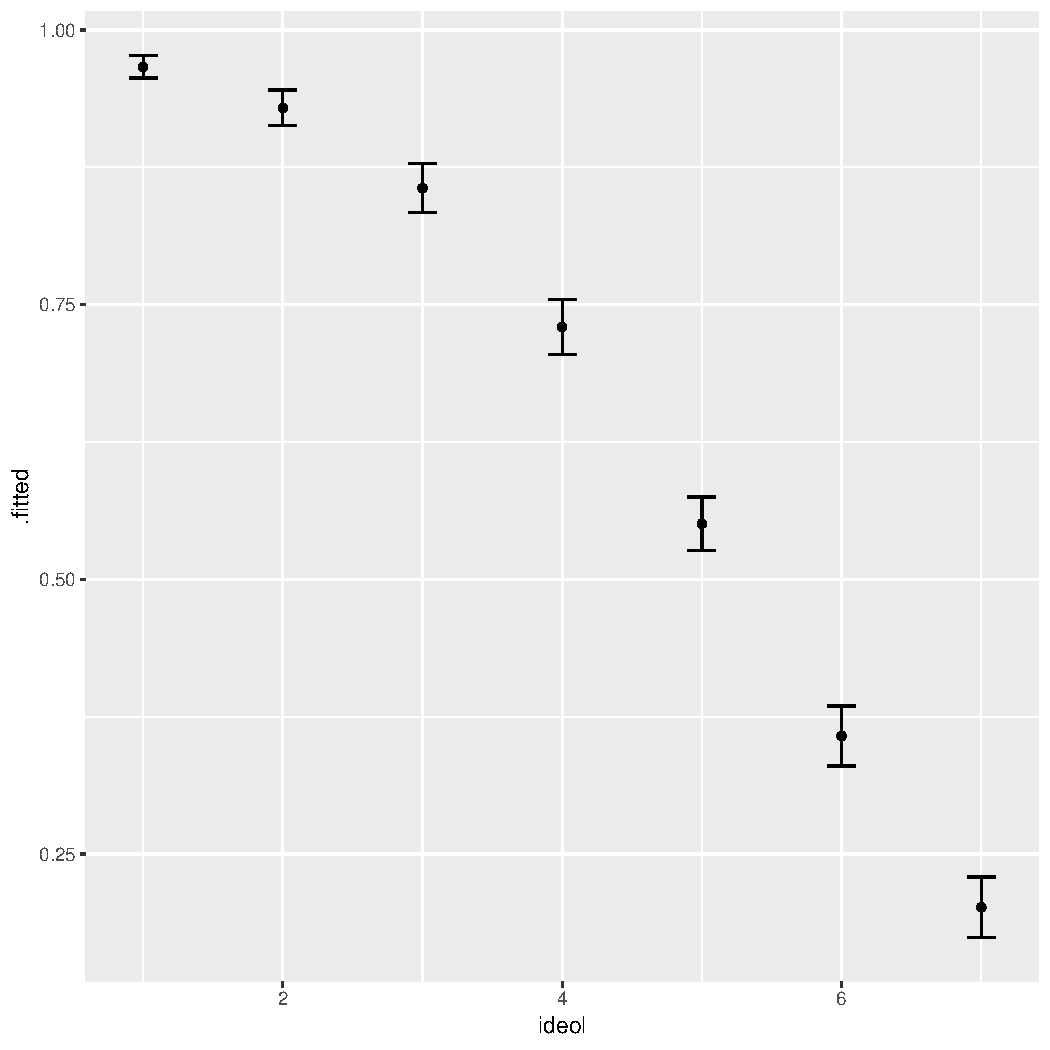
\includegraphics[width=4in]{16_Logit/logitplot.pdf}%filename
        \caption{Predicted Probability of believing that Greenhouse
          Gases cause Climate Change by Ideology \label{fig:logitplot}}
\end{figure}   
			                  
\noindent We can see that as respondents become more conservative, the probability of believing that climate change is man-made decreases at what appears to be an increasing rate.   

\section{Summary}

As an analysis and research tool, logit modeling expands your capabilities beyond those that can reasonably be estimated with OLS. Now you can accommodate  models with binary dependent variables. Logit models are a family of generalized linear models that are useful for predicting the odds or probabilities, of outcomes for binary dependent variables. This chapter has described the manner in which logits are calculated, how model fit can be  characterized, and several methods for making the logit results readily interpretable.

Perhaps one of the greatest difficulties in applications of logit models is the clear communication of the meaning of the results. The estimated coefficients show the change in the log of the odds for a one unit increase in the $X$ variable -- not the usual way to describe effects. But, as described in this chapter, these estimated coefficients can be readily transformed into changes in the odds, or the logit itself can be ``reversed" to provide estimated probabilities.  Of particular utility are logit graphics, showing the estimated shift in $Y$ from values of zero to one; the estimated probabilities of $Y$=1 for cases with specified combinations of values in the $X$ variables; and estimates of the ranges of probabilities for $Y$=1 across the ranges of values in any $X$. 

In sum, the use of logit models will expand your ability to test hypotheses to include a range of outcomes that are binary in nature. Given that a great deal of the phenomena of interest in the policy and social sciences are of this kind, you will find this capability to be an important part of your research toolkit. 

\part{Appendices}




\chapter{Appendix: Basic R}

This Appendix willl introduce you to the basics of programming languages, such as  R, as well as explain why we have chosen to use R in our course and this textbook. Then we will provide you with some basic programming skills in R that are generally unrelated to the use of R as a statistical software such as downloading, reading, manipulating and writing data. In so doing, we will prepare and introduce you to the data used throughout the book and for associated exercises. 

\section{Introduction to R}

R is a language and environment for statistical computing and graphics. It was developed at Bell Laboratories (formerly AT\&T, now Lucent Technologies) by John Chambers and colleagues. It is based off of another language called S. R is an integrated suite of software facilities for data manipulation, calculation and graphical display. It includes:
\begin{itemize}
\item an effective data handling and storage facility,
\item a suite of operators for calculations on arrays, in particular matrices,
\item a large, coherent, integrated collection of intermediate tools for data analysis,
\item graphical facilities for data analysis and display either on-screen or on hardcopy, and
\item a well-developed, simple and effective programming language which includes conditionals, loops, user-defined recursive functions and input and output facilities.
\end{itemize}

R is a powerful and effective tool for computing, statistics and analysis, and producing graphics. However, many applications exist that can do these or similar things. R has a number of benefits that make it particularly useful for a book such as this. First, similar to the book itself, R is open source and free. This comes with a set of associated advantages. Free is, of course, the best price. Additionally, this allows you, the student or reader, to take this tool with you wherever you go. You are not dependent on your employer to buy or have a license of a particular software. This is especially relevant as other software with similar functionality often cost hundreds, if not thousands, of dollars for a single license. The open source nature of R has resulted in a robust set of users, across a wide variety of disciplines including political science, who are constantly updating and revising the language. R therefore has some of the most up-to-date and innovative functionality and methods available to its users should they know where to look. Within R, these functions and tools are often implemented as packages. Packages allow advanced users of R to contribute statistical methods and computing tools to the general users of R. These packages are reviewed and vetted and then added to the CRAN repository. Later, we will cover some basic packages we will use throughout the book. The CRAN repository is where we will download R.

\section{Downloading R and RStudio}

In this section we will provide instructions to downloading R and RStudio. RStudio is an integrated development environment (IDE) that makes R a bit more user-friendly. In the class associated with this text, RStudio will primarily be used; however, it should be noted other IDEs exist for R. Additionally, R can be used without the aid of an IDE should you decide to do so. 

First to download R we need to go to the R project website repository as mentioned before. This can be found \href{https://www.r-project.org/}{here}. This website has many references relevant to R Users. To download R, go to the CRAN \href{https://cran.r-project.org/mirrors.html}{here}. It is recommended that individuals choose the mirror that is nearest their actual location. (For the purposes of this class, we therefore recommend the Revolution Analytics mirror in Dallas though really any Mirror will do just fine.) Once here, you will want to click the link that says download R for your relevant operating system (Mac, Windows, or Linux). On the next page, you will click the link that says install R for the first time. This will open a page that should look something like this:

\begin{figure}[h]
\centering
\includegraphics[width = \textwidth]{17_Appendix/"Download Page".png}
\caption{R Download Page
\label{fig:rdp}}
\end{figure}

Here you will click the Download R link at the top of the page. This should download the Installation Wizard for R. Once this has begun, you will click through the Wizard. You can choose where to locate your copy of R, to create a desktop icon, among other things. Unless you know what you are doing or have particular preferences, the default settings will work and are preferred. 

At this point, you now have R downloaded on your device and can be pretty much ready to go. However, as stated previously, we are also going to show you how to download RStudio. You will find the site to download RStudio \href{https://www.rstudio.com/products/rstudio/download2/}{here}. It should look like this: 

\begin{figure}[h!]
\centering
\includegraphics[width=\textwidth]{17_Appendix/"RStudio Download Page".png}
\caption{RStudio Download Page 
\label{fig:rsdp}}
\end{figure}

\begin{figure}[h]
\centering
\includegraphics[width=\textwidth]{17_Appendix/"RStudio Download Page 2".png}
\caption{Bottom of RStudio Download Page 
\label{fig:brsdp}}
\end{figure}


Here you will scroll down until it looks like \ref{fig:brsdp}. Then you will want to use the links under the installer subtitle for your relevant operating system again. You do not need to use the links under the tarball/zip header. As with R, you should then simply follow the default locations and settings in the Installer of RStudio. As we said before, RStudio simply makes the use of R a little easier and more user friendly. It includes some of the functionality that often makes other statistical softwares preferred for initially teaching students statistics. Once you have R and RStudio downloaded, you are prepared to dive right in. However, before we do that we want to introduce you to some common terminology in the fields of programming as well as statistics that may be helpful in your understanding of R.

\section{Introduction to Programming}

R is a programming language similar to other languages such a Java, Python, and others in many respects. As such it comes with a terminology that may be unfamilair to most readers. In this section we introduce some of this terminology in order to give readers the working knowledge necessary to utilize the rest of the book to the best of its ability. One particular thing to note is that R is an \textbf{object oriented} programming language. This means the program is organized around the data we are feeding it rather than the logical procedures used to manipulate it. This introduces to the important concept of \textbf{data types and structures}. For R, and programming languages generally, there is no agreed upon or common usage of the terms \textbf{data type} versus \textbf{data structure}. For the purposes of this book, we will attempt to use the term \textbf{data structure} to refer to the ways in which data are organized and \textbf{data type} to the characteristics of the particular data within the strucutre. \textbf{Data types} make up the building blocks of data strutures. There are many data types; we will cover only the most common ones that are releavant to our book. The first is the \textbf{character} type. This is simply a single Unicode character. The second is a \textbf{string}. Strings are simply a set of characters. This data type can contain, among other things, respodents' names and other common text data. The next data type is the \textbf{logical} type. This type simple indicates whether or not a statement or condition is True or False. It is often represented as a 0/1 in many cases. Finally, there are \textbf{numerical} data types. One is the \textbf{integer} which is, as you may recall, a number with nothing after the decimal point. On the other hand, the \textbf{float} data type allows for numbers with numbers before and after the decimal point.

In R, there are  a plethora of data structures to structure our data types. We will focus on a few common ones. Probably the simplest data structure is a \textbf{vector}. A vector is an object where all elements are of the same data type. A \textbf{scalar} is simply a vector with only one value. For the purposes of this book, a variable is often represented as a vector or the column of a dataset. \textbf{Factors} are vectors with a fixed set of values called levels. A common example of this in the social sciences is sex with only two levels- male or female. A \textbf{matrix} is a two dimensional collection of values, all of the same type. Thus, a matrix is simply a collection of vectors. An \textbf{array} is a matrix with more than 2-dimensions. The data structure we will use most is a \textbf{dataframe}. A data frame is simply a matrix but the values do not all have to be the same type. Therefore, a dataframe can have a vector that is text data type, a vector that is numerical data type, and a vector that is a logical data type or any possible combination. Finally, \textbf{lists} are collections of these data structures. They are essentially a method of gathering together a set of dataframes, matrices, etc. These will not commonly be used in our book but are important in many applications. Now that we have covered the basic types and structures of data we are going to explain how to get data into R. 

\section{Uploading/Reading Data}

R can handle a variety of different file types as data. The primary type that will be used for the book and accompanying course is a comma separated file or .csv file type. A CSV is a convenient file type that is portable across many operating platforms (Mac, Windows, etc) as well as statistical/data manipulation softwares. Other common file types are text (.txt) and Excel files (.xls or .xlsx). R also has its own file type called a R data file with the .RData extension. Other statistical softwares also have their own file types such as Stata's .dta file extension. R has built in functionality to deal with .csv and .txt as well as a few other file extensions. Uploading other data types requires special packages (haven, foreign, and readxl are popular for these purposes). These methods work for uploading files from the hard drives on our computers. You can also directly download data from the internet in R from a variety of sources and using a variety of packages. 

For the purposes of the book, we will acquire our data by going \href{http://crcm.ou.edu/epscordata/}{here}. You will then put your e-mail where it says Request Data. You should then receive an e-mail with the data attached as a .csv file. First, you will want to download this data onto your computer. We recommend creating a folder specifically for the book and its data (and if you're in the class for your classwork). This file will be your working directory. For each script we run in class, you will have to set your working directory. An easy way to do this in RStudio is to go to the Session tab. Scroll about halfway down to the option that says ``Set Working Directory" and then click ``Choose Directory..." This then opens up an explorer or search panel that allows you to choose the folder that you have saved the data in. This will then create a line of code in the console of RStudio that you then copy and paste into the Code editor to set the working directory for your data. You then run this code by hitting Ctrl+Enter on the highlighted line. 

Once this has been done, it is a good idea to check your directory. One easy way to do this is the `list.files()` command which will list all files saved in the folder you have set as your working directory. If you have done this correctly, the data you downloaded should show up as a file. Once you have done this, uploading the data will be easy. Simply write one line of code:

\begin{knitrout}
\definecolor{shadecolor}{rgb}{0.969, 0.969, 0.969}\color{fgcolor}\begin{kframe}
\begin{alltt}
\hlstd{newdat} \hlkwb{<-} \hlkwd{read.csv}\hlstd{(}\hlstr{"w1_w13_longdata.csv"}\hlstd{)}
\end{alltt}
\end{kframe}
\end{knitrout}

\begin{knitrout}
\definecolor{shadecolor}{rgb}{0.969, 0.969, 0.969}\color{fgcolor}\begin{kframe}
\begin{alltt}
\hlkwd{list.files}\hlstd{()}
\end{alltt}
\end{kframe}
\end{knitrout}

This line of code loads our data saved as a .csv into R and saves it as an object (remember, object oriented programming from earlier) that we call ds (short for dataset). This is the convention for the entire book. Now that we have the data downloaded from the internet and uploaded into R we are going to introduce you to some brief data manipulation techniques.

\section{Data Manipulation in R}

R is a very flexible tool for manipulating data into various subsets and forms. There are many useful packages and functions for doing this including the dplyr package, tidyr package, and more. R and its packages will allow users to transform their data from long to wide formats, remove NA values, recode variables, etc. In order to make the downloaded date more manageable for the book, we are going to do two things. First we want to restrict our data to one wave. The data we downloaded represent many waves of a quarterly survey that is sent to a panel of Oklahoma residents on weather, climate and policy preferences. This book will not venture into panel data analysis or time series analysis as it is an introductory text and therefore we want simply one cross section of data for our analysis. This can be done with one simple line of code:

\begin{knitrout}
\definecolor{shadecolor}{rgb}{0.969, 0.969, 0.969}\color{fgcolor}\begin{kframe}
\begin{alltt}
\hlcom{# newdat<-subset(newdat, newdat$wave_id == 'Wave 12 (Fall}
\hlcom{# 2016)')}
\end{alltt}
\end{kframe}
\end{knitrout}

What this line of code is doing is creating an object, that we have again named ds in order to overwrite our old object, that has only the 12th wave of data from the survey. In effect, this is removing all rows in which waveid, the variable that indicates the survey wave, does not equal twelve. Across these many waves, many different questions are asked and various variables are collected. We now want to remove all columns or variables that were not collected in wave twelve. This can also be done with one line of code:

\begin{knitrout}
\definecolor{shadecolor}{rgb}{0.969, 0.969, 0.969}\color{fgcolor}\begin{kframe}
\begin{alltt}
\hlcom{# newdat<-newdat[, !apply(is.na(newdat), 2, all)]}
\end{alltt}
\end{kframe}
\end{knitrout}

This line of code is a bit more complicated but what it is essentially doing is first searching all of ds for NA values using the is.na function. It is then returning a logical value of TRUE or FALSE---if a cell does have an NA then the value returned is TRUE and vice versa. It is then searching by column which is represented by the number 2 (rows are represented by the number 1) to see if all of the values are TRUE or FALSE. This then returns a logical value for the column, either TRUE if all of the rows/cells are NAs or FALSE if at least one row/cell in the column is not an NA. The ! is then reversing the TRUE and FALSE meanings. Now TRUE means a column that is not all NA and therefore one we want to keep. Finally, the brackets are another way to subset our data set. This allows us to keep all columns where the returned value is TRUE or not all values were NA. Because we are concerned with columns, we write the function after the comma. If we wanted to do a similar thing but with rows we would put the function before the comma. Finally, now that we have done this we want to save this dataset to our working directory which will be explained in the following section

\section{Saving/Writing Data}

Saving or writing data that we have manipulated is a useful tool. It allows us to easily share datasets we have created with others. This is useful for collaboration, especially with other users who may not use R. Additionally, this will be useful for the book as our new dataset is the one that will be worked with throughout the book. This dataset is much smaller than the one we originally downloaded and therefore will allow for quicker load times as well as hopefully reduce potential confusion. The code to save this data set is rather simple as well:

\begin{knitrout}
\definecolor{shadecolor}{rgb}{0.969, 0.969, 0.969}\color{fgcolor}\begin{kframe}
\begin{alltt}
\hlcom{# write.csv(newdat, 'Class Data Set.csv')}
\end{alltt}
\end{kframe}
\end{knitrout}

This line of code allows us to save the dataset we created and saved in the object named ds as a new .csv file in our working directory called Class Data Set. Having successfully downloaded R and RStudio, learned some basic programming and data manipulation techniques, and saved the class data set to your working directory you are ready to use the rest of the book to its fullest potential. 

\section{The Tidyverse}

This edition of the book employs the tidyverse family of R functions for both statistical analysis and data visualization. The tidyverse is a collection of functions that provide an efficient, consistent, and intuitive method of both working with your data and visualizing it. Packages like dplyr are used as the primary method of data exploration and wrangling, and ggplot2 is used for visualization. More information can be found about the tidyverse at www.tidyverse.org. 




\end{document}

